\section{Group -- Zone Forced Air Units}\label{group-zone-forced-air-units}

\paragraph{Schedules And Availability Manager}\label{schedules-and-availability-manager}
Regarding component schedules, the general rule is don't schedule any components except the supply fan and the corresponding availability manager(s). Beyond that, every component should always be available and let the controls determine what runs or doesn't run. If a component other than the supply fan is scheduled off, then it will remain off even if the night cycle manager turns on the system.

\subsection{ZoneHVAC:IdealLoadsAirSystem}\label{zonehvacidealloadsairsystem}

The simplest piece of zone equipment is the ZoneHVAC:IdealLoadsAirSystem component. ZoneHVAC:IdealLoadsAirSystem is used in situations where the user wishes to study the performance of a building without modeling a full HVAC system. In such a case, the Ideal Loads Air System is usually the sole conditioning component: the user does not need to specify air loops, water loops, etc. All that is needed for the ideal system are zone controls, zone equipment configurations, and the ideal loads system component. The use of a return plenum is optional and will require use of the AirloopHVAC:ReturnPlenum object.

This component can be operated with infinite or finite heating and cooling capacity. For either mode -- infinite or limited capacity -- the user can also specify on/off schedules for heating and cooling and outdoor air controls. There are also optional controls for dehumidification, humidification, economizer, and heat recovery. This component may be used in combination with other HVAC equipment serving the same zone.

This component can be thought of as an ideal unit that mixes air at the zone exhaust condition (or plenum outlet condition when a plenum is attached) with the specified amount of outdoor air and then adds or removes heat and moisture at 100\% efficiency in order to produce a supply air stream at the specified conditions. The energy required to condition the supply air is metered and reported as \hyperref[districtheating]{DistrictHeating} and \hyperref[districtcooling]{DistrictCooling}.

\textbf{Notes:} The ideal loads system uses the zone return node or an optional zone exhaust node to extract air from the zone. When the AirloopHVAC:ReturnPlenum is used the inlet of the ideal loads system is connected to the plenum outlet air node while the outlet of the ideal loads system is connected to a zone inlet node. The node name connected between the zone exhaust air node and plenum inlet air node must match in the \hyperref[zonehvacequipmentconnections]{ZoneHVAC:EquipmentConnections} and AirloopHVAC:ReturnPlenum objects. Every zone served by an HVAC component must have a return air node, even though this node may not be connected to anything. If more than one ideals loads air systems are connected to the same AirloopHVAC:ReturnPlenum then one of the ideal loads air systems will connect to the ZoneHVAC:ReturnPlenum outlet air node and the remaining ideal loads air systems connected to the same return plenum will connect to the ZoneHVAC:ReturnPlenum induced air outlet nodes.

The ideal loads system was significantly expanded in version 7.0 (October 2011). As part of this upgrade, any change in the moisture content of the supply air stream results in a latent cooling (dehumidification) or latent heating (humidification) load which is metered as \hyperref[districtcooling]{DistrictCooling} and \hyperref[districtheating]{DistrictHeating} energy consumption. Prior to version 7.0, when the ideal loads system was in heating mode, only the energy for sensible heating was metered. This results in significant changes in reported energy use compared to earlier versions, especially when using the \textbf{\emph{ConstantSupplyHumidityRatio}} option for Humidification Control Type.

Older idf files which are transitioned to version 7.0 will automatically be set to use the \textbf{\emph{ConstantSupplyHumidityRatio}} option for both dehumidification and humidification controls, because this is equivalent to the controls used in the older version of this system. However, the user should review all of the humidity control options and select the one which best reflects the goal of the simulation.

\subsubsection{Inputs}\label{inputs-056}

\paragraph{Field: Name}\label{field-name-054}

A unique user assigned name for each ideal loads air system component.~ This name is referenced in a \hyperref[zonehvacequipmentlist]{ZoneHVAC:EquipmentList} object.

\paragraph{Field: Availability Schedule Name}\label{field-availability-schedule-name-020}

This alpha field defines the name of the schedule (ref: Schedule) that denotes whether or not this component is available to operate during a given time period. If the schedule value is greater than zero then the system is available to operate; otherwise, the system is unavailable for that time period. If this field is blank, the schedule has values of 1 for all time periods.

\paragraph{Field: Zone Supply Air Node Name}\label{field-zone-supply-air-node-name-001}

The name of the outlet air node of the ideal loads object. This should be the same as one of the zone air inlet nodes for the zone the ideal loads component is serving.

\paragraph{Field: Zone Exhaust Air Node Name}\label{field-zone-exhaust-air-node-name}

The name of the zone exhaust air node of the ideal loads object. This should be the same as one of the zone air exhaust nodes for the zone this component is serving. This node name is required if ZoneHVAC:IdealLoadsAirSystem is used in a zone which also has other forced air HVAC equipment. Otherwise this node name is optional but recommended.

\paragraph{Field: System Inlet Air Node Name}\label{system-inlet-air-node-name}

The optional name of the return plenum outlet node (or induced air outlet node) connected to the ideal loads object. When a return plenum is used, the previous fields for Zone Supply Air Node Name and Zone Exhaust Air Node Name are also required. When an AirloopHVAC:ReturnPlenum is connected to the Ideal Loads Air System the Zone Supply Air Node Name must match a zone air inlet node name and the Zone Exhaust Air Node Name must match a zone air exhaust node (see ZoneHAVC:EquipmentConnections object). The Zone Exhaust Air Node Name must also match an AirloopHVAC:ReturnPlenum inlet node name. In the AirloopHVAC:ReturnPlenum object, when more than one ideal loads air systems are connected to the same return plenum, the System Inlet Air Node Name for one of the ideal loads air systems must match the return plenum Outlet Node Name while all remaining ideal loads air systems, if more than one are connected, would enter the System Inlet Air Node Name in the return plenum Induced Air Outlet Node or \hyperref[nodelist]{NodeList} Name field (see Engineering Reference for schematic).

\paragraph{Field: Maximum Heating Supply Air Temperature}\label{field-maximum-heating-supply-air-temperature-000}

The maximum air temperature (\si{\degreeCelsius}) of the air used for heating the zone. The default is 50\si{\degreeCelsius} (122F).

\paragraph{Field: Minimum Cooling Supply Air Temperature}\label{field-minimum-cooling-supply-air-temperature-000}

The minimum air temperature (\si{\degreeCelsius}) of the air used for cooling the zone. The default is 13\si{\degreeCelsius} (55.4F).

\paragraph{Field: Maximum Heating Supply Air Humidity Ratio}\label{field-maximum-heating-supply-air-humidity-ratio-000}

The maximum humidity ratio (kg of water per kg of dry air) of the hot supply air. The default is 0.0156 kgWater/kgDryAir which corresponds to a 20\%RH at 50\si{\degreeCelsius} (122F) dry bulb.

\paragraph{Field: Minimum Cooling Supply Air Humidity Ratio}\label{field-minimum-cooling-supply-air-humidity-ratio-000}

The minimum humidity ratio (kg of water per kg of dry air) of the cool supply air. The default is 0.0077 kgWater/kgDryAir which corresponds to a 10\si{\degreeCelsius} (50F) dew point.

\paragraph{Field: Heating Limit}\label{field-heating-limit-000}

The input must be either \textbf{\emph{LimitFlowRate, LimitCapacity, LimitFlowRateAndCapacity}} or \textbf{\emph{NoLimit}}. \textbf{\emph{LimitFlowRate}} means that the heating supply air flow rate will be limited to the value specified in the next input field. \textbf{\emph{LimitCapacity}} means that the sensible heating capacity will be limited to the value specified in the Maximum Sensible Heating Capacity field. \textbf{\emph{LimitFlowRateAndCapacity}} means that both flow rate and capacity will be limited. \textbf{\emph{NoLimit}} (the default) means that there will not be any limit on the heating supply air flow rate or capacity and the subsequent two fields will be ignored.

\paragraph{Field: Maximum Heating Air Flow Rate}\label{field-maximum-heating-air-flow-rate-001}

The maximum heating supply air flow rate in cubic meters per second if heating limit is set to \textbf{\emph{LimitFlowRate or LimitFlowRateAndCapacity}} \emph{.} This field may be autosized. This field is ignored if heating limit is set to \textbf{\emph{NoLimit}} or \textbf{\emph{LimitCapacity}}.~ If blank, there is no limit.

\paragraph{Field: Maximum Sensible Heating Capacity}\label{field-maximum-sensible-heating-capacity-000}

The maximum allowed sensible heating capacity in Watts if Heating Limit is set to \textbf{\emph{LimitCapacity}} or \textbf{\emph{LimitFlowRateAndCapacity}}. This field may be autosized. If blank, there is no limit. If Heating Limit \emph{is set to \textbf{NoLimit}} or \textbf{\emph{LimitFlowRate}}, this field is ignored.

\paragraph{Field: Cooling Limit}\label{field-cooling-limit-000}

The input must be either \textbf{\emph{LimitFlowRate, LimitCapacity, LimitFlowRateAndCapacity}} or \textbf{\emph{NoLimit}}. \textbf{\emph{LimitFlowrate}} means that the cooling supply air flow rate will be limited to the value specified in the next input field. \textbf{\emph{LimitCapacity}} means that the total cooling capacity will be limited to the value specified in the Maximum Total Cooling Capacity field. \textbf{\emph{LimitFlowRateAndCapacity}} means that both flow rate and capacity will be limited. \textbf{\emph{NoLimit}} (the default) means that there will not be any limit on the cooling supply air flow rate or capacity and the subsequent two fields will be ignored.

\paragraph{Field: Maximum Cooling Air Flow Rate}\label{field-maximum-cooling-air-flow-rate-001}

The maximum cooling supply air flow rate in cubic meters per second if Cooling Limit is set to \textbf{\emph{LimitFlowRate}} or \textbf{\emph{LimitFlowRateAndCapacity}}\emph{.} This field may be autosized. This field is ignored if cooling limit is set to \textbf{\emph{NoLimit}} or \textbf{\emph{LimitCapacity}}. If blank, there is no limit. If \emph{Cooling Limit is set to \textbf{NoLimit},} this field is ignored\emph{.} This field is required if Outdoor Air Control Type is \textbf{\emph{TemperatureEconomizer}} in order to establish an upper limit on outdoor air flow when the economizer is active\textbf{\emph{.}}

\paragraph{Field: Maximum Total Cooling Capacity}\label{field-maximum-total-cooling-capacity-000}

The maximum allowed total (sensible plus latent) cooling capacity in Watts if Cooling Limit is set to \textbf{\emph{LimitCapacity}} or \textbf{\emph{LimitFlowRateAndCapacity}}. This field may be autosized. If blank, there is no limit. If Cooling Limit \emph{is set to \textbf{NoLimit}} or \textbf{\emph{LimitFlowRate}}\emph{,} this field is ignored\emph{.}

\paragraph{Field: Heating Availability Schedule Name}\label{field-heating-availability-schedule-name-001}

The name of a schedule (ref: Schedule) that denotes whether heating is available. A schedule value greater than 0 (usually 1 is used) indicates that heating and humidification are available. A value less than or equal to 0 (usually 0 is used) denotes that heating and humidification are not available. If blank, heating and humidification are always available.

\paragraph{Field: Cooling Availability Schedule Name}\label{field-cooling-availability-schedule-name-001}

The name of a schedule (ref: Schedule) that denotes whether cooling is available. A schedule value greater than 0 (usually 1 is used) indicates that cooling and dehumidification are available. A value less than or equal to 0 (usually 0 is used) denotes that cooling and dehumidification is not available. If blank, cooling and dehumidification are always available.

\paragraph{Field: Dehumidification Control Type}\label{field-dehumidification-control-type-002}

Select from \textbf{\emph{ConstantSensibleHeatRatio}}, \textbf{\emph{Humidistat, None, or ConstantSupplyHumidityRatio}}. \textbf{\emph{ConstantSensibleHeatRatio}} (the default) means that the ideal loads system will be controlled to meet the sensible cooling load, and the latent cooling rate will be computed using a constant sensible heat ratio (SHR) (see next field). \textbf{\emph{Humidistat}} means that there is a \hyperref[zonecontrolhumidistat]{ZoneControl:Humidistat} for this zone and the ideal loads system will attempt to meet the humidistat request (i.e.~will dehumidify according to the Dehumidifying Relative Humidity Schedule in the \hyperref[zonecontrolhumidistat]{ZoneControl:Humidistat} object). \textbf{\emph{None}} means that there is no dehumidification. \textbf{\emph{ConstantSupplyHumidityRatio}} means that during cooling the supply air will always be at the Minimum Cooling Supply Humidity Ratio. For \textbf{\emph{ConstantSensibleHeatRatio}} and \textbf{\emph{Humidistat}}, if the mixed air humidity ratio is less than the target humidity ratio, then the mixed air humidity ratio will be used. For all options, the supply air humidity ratio will never be allowed to exceed saturation at the supply dry bulb temperature.

The selected dehumidification control type is always applied when the unit is in cooling mode. If the unit is in deadband mode (not actively heating the supply air) control type \textbf{\emph{Humidistat}} will be active. If the unit is in heating mode, control type \textbf{\emph{Humidistat}} will be active if the Humidification Control Type field below is set to \emph{Humidistat} or \emph{None}.

This allows the ideal loads system to heat and dehumidify at the same time.

\paragraph{Field: Cooling Sensible Heat Ratio}\label{field-cooling-sensible-heat-ratio-000}

When the Dehumidification Control Type is set to \textbf{\emph{ConstantSensibleHeatRatio}} the ideal loads system will be controlled to meet the sensible cooling load, and the latent cooling rate will be computed using the value of Cooling Sensible Heat Ratio (SHR), where SHR = Sensible Cooling divided by Total Cooling (sensible plus latent). The default is 0.7. If Dehumidification Control Type is set to something other than \textbf{\emph{ConstantSensibleHeatRatio}} then this field will be ignored.

\paragraph{Field: Humidification Control Type}\label{field-humidification-control-type-000}

Select from \textbf{\emph{None}}, \textbf{\emph{Humidistat, or ConstantSupplyHumidityRatio}}. \textbf{\emph{None}} means that there is no humidification. \textbf{\emph{Humidistat}} means that there is a \hyperref[zonecontrolhumidistat]{ZoneControl:Humidistat} for this zone and the ideal loads system will attempt to meet the humidistat request (i.e., humidify according to the Humidifying Relative Humidity Setpoint Schedule in the \hyperref[zonecontrolhumidistat]{ZoneControl:Humidistat} object). \textbf{\emph{ConstantSupplyHumidityRatio}} means that during heating the supply air will always be at the Maximum Heating Supply Humidity Ratio. The default is \textbf{\emph{None}}. For \textbf{\emph{Humidistat}}, if the mixed air humidity ratio is greater than the target humidity ratio, then the mixed air humidity ratio will be used. For all options, the supply air humidity ratio will never be allowed to exceed saturation at the supply dry bulb temperature.

The selected humidification control type is always applied when the unit is in heating mode. If the unit is in deadband mode (not actively heating the supply air) control type \textbf{\emph{Humidistat}} will be active. If the unit is in cooling mode, control type \textbf{\emph{Humidistat}} will be active if the Dehumidification Control Type field above is set to \emph{Humidistat} or \emph{None}.

This allows the ideal loads system to cool and humidify at the same time.

\paragraph{Field: Design Specification Outdoor Air Object Name}\label{field-design-specification-outdoor-air-object-name-002}

This alpha field specifies the name of a \hyperref[designspecificationoutdoorair]{DesignSpecification:OutdoorAir} object which specifies the outdoor air requirements and schedule for this system. The outdoor air flow rate may also be affected by the next two fields, Demand Controlled Ventilation Type and Outdoor Air Economizer Type. If this field is blank, this system will have no outdoor air, and all outdoor air control and heat recovery options will be ignored..

\paragraph{Field: Outdoor Air Inlet Node Name}\label{field-outdoor-air-inlet-node-name-002}

This alpha field specifies the node name of the outdoor air inlet node. This node name is also specified in an \hyperref[outdoorairnode]{OutdoorAir:Node} or \hyperref[outdoorairnodelist]{OutdoorAir:NodeList} object. If this field is blank, a node name will be created internally.

\paragraph{Field: Demand Controlled Ventilation Type}\label{field-demand-controlled-ventilation-type-000}

This field, along with the Design Specification Outdoor Air Object (if used) specifies how the minimum outdoor air flow rate is calculated. The choices are: \textbf{\emph{None, OccupancySchedule or CO2Setpoint}}. The default is \textbf{\emph{None}}.

\begin{itemize}
\item
  \textbf{\emph{None}} means that the design occupancy level will be used when computing the minimum outdoor air flow rate based on the inputs in the Design Specification Outdoor Air Object (see previous field).
\item
  \textbf{\emph{OccupancySchedule}} means that the current occupancy level will be used when computing the minimum outdoor air flow rate based on the inputs in the Design Specification Outdoor Air Object (see previous field).
\item
  \textbf{\emph{CO2Setpoint}} means that the design occupancy level will be used when computing the minimum outdoor air flow rate based on the inputs in the Design Specification Outdoor Air Object (see previous field). In addition, the minimum outdoor air flow rate may be increased if necessary to maintain the level of indoor air carbon dioxide at or below the setpoint defined in a \hyperref[zonecontrolcontaminantcontroller]{ZoneControl:ContaminantController} object.
\end{itemize}

\paragraph{Field: Outdoor Air Economizer Type}\label{field-outdoor-air-economizer-type-000}

This field specifies if there is an outdoor air economizer. The choices are: \textbf{\emph{NoEconomizer, DifferentialDryBulb,}} or \textbf{\emph{DifferentialEnthalpy}}. The default is \textbf{\emph{NoEconomizer}}. \textbf{\emph{DifferentialDryBulb}} and \textbf{\emph{DifferentialEnthalpy}} mean that the economizer will increase the outdoor air flow rate above the minimum outdoor air flow (see fields Design Specification Outdoor Air Object Name and Demand Controlled Ventilation Type) when there is a cooling load and the outdoor air temperature or enthalpy is below the zone exhaust air temperature or enthalpy. The \textbf{\emph{DifferentialDryBulb}} and \textbf{\emph{DifferentialEnthalpy}} options require that the Maximum Cooling Air Flow Rate be specified which will be used as the limit for maximum outdoor air flow rate.

\paragraph{Field: Heat Recovery Type}\label{field-heat-recovery-type-000}

Select from \textbf{\emph{None}}, \textbf{Sensible}, or \textbf{\emph{Enthalpy}}. \textbf{\emph{None}} means that there is no heat recovery. \textbf{\emph{Sensible}} means that there is sensible heat recovery whenever the zone exhaust air temperature is more favorable than the outdoor air temperature. \textbf{\emph{Enthalpy}} means that there is latent and sensible heat recovery whenever the zone exhaust air enthalpy is more favorable than the outdoor air enthalpy. The default is \textbf{\emph{None}}.

\paragraph{Field: Sensible Heat Recovery Effectiveness}\label{field-sensible-heat-recovery-effectiveness-000}

The sensible heat recovery effectiveness, where effectiveness is defined as the change in supply temperature divided by the difference in entering supply and relief air temperatures. The default is 0.70.

\paragraph{Field: Latent Heat Recovery Effectiveness}\label{field-latent-heat-recovery-effectiveness-000}

The latent heat recovery effectiveness, where effectiveness is defined as the change in supply humidity ratio divided by the difference in entering supply and relief air humidity ratios. The default is 0.65.

\paragraph{Field: Design Specification ZoneHVAC Sizing Object Name}\label{field-design-specification-zonehvac-sizing-object-name-000}

This optional input field is the name of a \hyperref[designspecificationzonehvacsizing]{DesignSpecification:ZoneHVAC:Sizing} object. The name must correspond to unique name of a \hyperref[designspecificationzonehvacsizing]{DesignSpecification:ZoneHVAC:Sizing} object. A Design Sepcification Zone HVAC Sizing object defines scalable sizing methods for sizing input fields such as Maximum Heating Air Flow Rate and Maximum Cooling Air Flow Rate in a Ideal Load Air System zone HVAC object. The scaled maximum heating and cooling air flow rates are used to size the heating and cooling capacities.

An example of this object in an IDF is:

\begin{lstlisting}

  ZoneHVAC:IdealLoadsAirSystem,
      Zone1 Ideal Loads System, !- Name
      AlwaysOn,                !- Availability Schedule Name
      Zone1 Ideal Loads Supply Node, !- Zone Supply Air Node Name
      Zone1 Ideal Loads Return Node, ! Zone Exhaust Air Node Name
      50,                      !- Maximum Heating Supply Air Temperature {C}
      13,                      !- Minimum Cooling Supply Air Temperature {C}
      0.0156,                  !- Maximum Heating Supply Air Humidity Ratio {kgWater/kgDryAir}
      0.0077,                  !- Minimum Cooling Supply Air Humidity Ratio {kgWater/kgDryAir}
      NoLimit,                 !- Heating Limit
      ,                        !- Maximum Heating Air Flow Rate {m3/s}
      ,                        !- Maximum Sensible Heating Capacity {W}
      NoLimit,                 !- Cooling Limit
      ,                        !- Maximum Cooling Air Flow Rate {m3/s}
      ,                        !- Maximum Total Cooling Capacity {W}
      ,                        !- Heating Availability Schedule Name
      ,                        !- Cooling Availability Schedule Name
      ConstantSensibleHeatRatio,  !- Dehumidification Control Type
      0.7,                     !- Cooling Sensible Heat Ratio
      None,                    !- Humidification Control Type
      Office OA Specification, !- Design Specification Outdoor Air Object Name
      Zone1 Ideal Loads OA Inlet Node, !- Outdoor Air Inlet Node Name
      None,                    !- Demand Controlled Ventilation Type
      NoEconomizer,            !- Outdoor Air Economizer Type
      Enthalpy,                !- Heat Recovery Type
      0.70,                    !- Sensible Heat Recovery Effectiveness
      0.65;                    !- Latent Heat Recovery Effectiveness
\end{lstlisting}

\subsubsection{Outputs}\label{outputs-043}

The Ideal Loads air system outdoor air load variables are only calculated when there is active heating or cooling (or humidification/dehumidification).

\begin{itemize}
\item
  HVAC,Sum,Zone Ideal Loads Supply Air Sensible Heating Energy {[}J{]}
\item
  HVAC,Sum,Zone Ideal Loads Supply Air Total Heating Energy {[}J{]}
\item
  HVAC,Sum,Zone Ideal Loads Supply Air Sensible Cooling Energy {[}J{]}
\item
  HVAC,Sum,Zone Ideal Loads Supply Air Latent Cooling Energy {[}J{]}
\item
  HVAC,Sum,Zone Ideal Loads Supply Air Total Cooling Energy {[}J{]}
\item
  HVAC,Sum,Zone Ideal Loads Supply Air Latent Heating Energy {[}J{]}
\item
  HVAC,Sum,Zone Ideal Loads Zone Sensible Heating Energy {[}J{]}
\item
  HVAC,Sum,Zone Ideal Loads Zone Latent Heating Energy {[}J{]}
\item
  HVAC,Sum,Zone Ideal Loads Zone Total Heating Energy {[}J{]}
\item
  HVAC,Sum,Zone Ideal Loads Zone Sensible Cooling Energy {[}J{]}
\item
  HVAC,Sum,Zone Ideal Loads Zone Latent Cooling Energy {[}J{]}
\item
  HVAC,Sum,Zone Ideal Loads Zone Total Cooling Energy {[}J{]}
\item
  HVAC,Sum,Zone Ideal Loads Outdoor Air Sensible Heating Energy {[}J{]}
\item
  HVAC,Sum,Zone Ideal Loads Outdoor Air Latent Heating Energy {[}J{]}
\item
  HVAC,Sum,Zone Ideal Loads Outdoor Air Total Heating Energy {[}J{]}
\item
  HVAC,Sum,Zone Ideal Loads Outdoor Air Sensible Cooling Energy {[}J{]}
\item
  HVAC,Sum,Zone Ideal Loads Outdoor Air Latent Cooling Energy {[}J{]}
\item
  HVAC,Sum,Zone Ideal Loads Outdoor Air Total Cooling Energy {[}J{]}
\item
  HVAC,Sum,Zone Ideal Loads Heat Recovery Sensible Heating Energy {[}J{]}
\item
  HVAC,Sum,Zone Ideal Loads Heat Recovery Latent Heating Energy {[}J{]}
\item
  HVAC,Sum,Zone Ideal Loads Heat Recovery Total Heating Energy {[}J{]}
\item
  HVAC,Sum,Zone Ideal Loads Heat Recovery Sensible Cooling Energy {[}J{]}
\item
  HVAC,Sum,Zone Ideal Loads Heat Recovery Latent Cooling Energy {[}J{]}
\item
  HVAC,Sum,Zone Ideal Loads Heat Recovery Total Cooling Energy {[}J{]}
\item
  HVAC,Average,Zone Ideal Loads Supply Air Sensible Heating Rate {[}W{]}
\item
  HVAC,Average,Zone Ideal Loads Supply Air Latent Heating Rate {[}W{]}
\item
  HVAC,Average,Zone Ideal Loads Supply Air Total Heating Rate {[}W{]}
\item
  HVAC,Average,Zone Ideal Loads Supply Air Sensible Cooling Rate {[}W{]}
\item
  HVAC,Average,Zone Ideal Loads Supply Air Latent Cooling Rate {[}W{]}
\item
  HVAC,Average,Zone Ideal Loads Supply Air Total Cooling Rate {[}W{]}
\item
  HVAC,Average,Zone Ideal Loads Zone Sensible Heating Rate {[}W{]}
\item
  HVAC,Average,Zone Ideal Loads Zone Latent Heating Rate {[}W{]}
\item
  HVAC,Average,Zone Ideal Loads Zone Total Heating Rate {[}W{]}
\item
  HVAC,Average,Zone Ideal Loads Zone Sensible Cooling Rate {[}W{]}
\item
  HVAC,Average,Zone Ideal Loads Zone Latent Cooling Rate {[}W{]}
\item
  HVAC,Average,Zone Ideal Loads Zone Total Cooling Rate {[}W{]}
\item
  HVAC,Average,Zone Ideal Loads Outdoor Air Sensible Heating Rate {[}W{]}
\item
  HVAC,Average,Zone Ideal Loads Outdoor Air Latent Heating Rate {[}W{]}
\item
  HVAC,Average,Zone Ideal Loads Outdoor Air Total Heating Rate {[}W{]}
\item
  HVAC,Average,Zone Ideal Loads Outdoor Air Sensible Cooling Rate {[}W{]}
\item
  HVAC,Average,Zone Ideal Loads Outdoor Air Latent Cooling Rate {[}W{]}
\item
  HVAC,Average,Zone Ideal Loads Outdoor Air Total Cooling Rate {[}W{]}
\item
  HVAC,Average,Zone Ideal Loads Heat Recovery Sensible Heating Rate {[}W{]}
\item
  HVAC,Average,Zone Ideal Loads Heat Recovery Latent Heating Rate {[}W{]}
\item
  HVAC,Average,Zone Ideal Loads Heat Recovery Total Heating Rate {[}W{]}
\item
  HVAC,Average,Zone Ideal Loads Heat Recovery Sensible Cooling Rate {[}W{]}
\item
  HVAC,Average,Zone Ideal Loads Heat Recovery Latent Cooling Rate {[}W{]}
\item
  HVAC,Average,Zone Ideal Loads Heat Recovery Total Cooling Rate {[}W{]}
\item
  HVAC,Sum,Zone Ideal Loads Economizer Active Time {[}hr{]}
\item
  HVAC,Sum,Zone Ideal Loads Heat Recovery Active Time {[}hr{]}
\item
  HVAC,Average,Zone Ideal Loads Hybrid Ventilation Available Status {[]}
\item
  HVAC,Average,Zone Ideal Loads Outdoor Air Mass Flow Rate {[}kg/s{]}
\item
  HVAC,Average,Zone Ideal Loads Outdoor Air Standard Density Volume Flow Rate {[}m3/s{]}
\item
  HVAC,Average,Zone Ideal Loads Supply Air Mass Flow Rate {[}kg/s{]}
\item
  HVAC,Average,Zone Ideal Loads Supply Air Standard Density Volume Flow Rate {[}m3/s{]}
\item
  HVAC,Average,Zone Ideal Loads Supply Air Temperature {[}\si{\degreeCelsius}{]}
\item
  HVAC,Average,Zone Ideal Loads Supply Air Humidity Ratio {[}kgWater/kgDryAir{]}
\item
  HVAC,Average,Zone Ideal Loads Mixed Air Temperature {[}\si{\degreeCelsius}{]}
\item
  HVAC,Average,Zone Ideal Loads Mixed Air Humidity Ratio {[}kgWater/kgDryAir{]}
\end{itemize}

\paragraph{Ideal Loads Output Variable Overview}\label{ideal-loads-output-variable-overview}

All of the ZoneHVAC:IdealLoadsAirSystem loads and energy use are reported for Sensible Heating, Latent Heating, Total Heating, Sensible Cooling, Latent Cooling, and Total Cooling. To explain the relationship between the various outputs, Total Cooling Energy will be used. Note that the outdoor air load variables are only calculated when there is active heating or cooling (or humidification/dehumidification).

\emph{Zone Ideal Loads Supply Air Total Cooling Energy} is the district cooling energy consumed by the ideal loads system ``cooling coil'' to cool and dehumidify the supply air.

\emph{Zone Ideal Loads Zone Total Cooling Energy} is the total (sensible plus latent) cooling energy delivered to the zone. If there is no outdoor air, then \emph{Zone Ideal Loads Supply Air Total Cooling Energy = Zone Ideal Loads Zone Total Cooling Energy.}

\emph{Zone Ideal Loads Outdoor Air Total Cooling Energy} is the total (sensible plus latent) cooling energy required to cool the outdoor air to the zone exhaust air temperature and humidity ratio.

\emph{Zone Ideal Loads Heat Recovery Total Cooling Energy} is the total (sensible plus latent) cooling energy supplied by heat recovery. This offsets a portion of the \emph{Zone Ideal Loads Outdoor Air Total Cooling Energy}.

When the economizer is not active, these values are related by the following equation:

\emph{Zone Ideal Loads Supply Air Total Cooling Energy + Zone Ideal Loads Heat Recovery Total Cooling Energy = Zone Ideal Loads Zone Total Cooling Energy+ Zone Ideal Loads Outdoor Air Total Cooling Energy}

\paragraph{Zone Ideal Loads Supply Air Sensible Heating Energy {[}J{]}}\label{zone-ideal-loads-supply-air-sensible-heating-energy-j}

\paragraph{Zone Ideal Loads Supply Air Sensible Heating Rate {[}W{]}}\label{zone-ideal-loads-supply-air-sensible-heating-rate-w}

The sensible heating energy (or rate) added to raise the temperature of the mixed air stream to the temperature of the supply air stream. This is the ideal ``heating coil'' load.

\paragraph{Zone Ideal Loads Supply Air Latent Heating Energy {[}J{]}}\label{zone-ideal-loads-supply-air-latent-heating-energy-j}

\paragraph{Zone Ideal Loads Supply Air Latent Heating Rate {[}W{]}}\label{zone-ideal-loads-supply-air-latent-heating-rate-w}

The latent heating energy (or rate) added to raise the humidity ratio of the mixed air stream to the temperature of the supply air stream. This is the ideal ``humidifier'' load.

\paragraph{Zone Ideal Loads Supply Air Total Heating Energy {[}J{]}}\label{zone-ideal-loads-supply-air-total-heating-energy-j}

\paragraph{Zone Ideal Loads Supply Air Total Heating Rate {[}W{]}}\label{zone-ideal-loads-supply-air-total-heating-rate-w}

The total (sensible and latent) heating energy (or rate) added to raise the mixed air stream to the temperature and humidity ratio of the supply air stream. \emph{Zone Ideal Loads Supply Air Total Heating Energy} is metered as DistrictHeating energy.

\paragraph{Zone Ideal Loads Supply Air Sensible Cooling Energy {[}J{]}}\label{zone-ideal-loads-supply-air-sensible-cooling-energy-j}

\paragraph{Zone Ideal Loads Supply Air Sensible Cooling Rate {[}W{]}}\label{zone-ideal-loads-supply-air-sensible-cooling-rate-w}

The sensible cooling energy (or rate) removed to lower the temperature of the mixed air stream to the temperature of the supply air stream. This is the ideal ``cooling coil'' sensible load.

\paragraph{Zone Ideal Loads Supply Air Latent Cooling Energy {[}J{]}}\label{zone-ideal-loads-supply-air-latent-cooling-energy-j}

\paragraph{Zone Ideal Loads Supply Air Latent Cooling Rate {[}W{]}}\label{zone-ideal-loads-supply-air-latent-cooling-rate-w}

The latent cooling energy (or rate) removed to lower the humidity ratio of the mixed air stream to the temperature of the supply air stream. This is the ideal ``cooling coil'' latent load.

\paragraph{Zone Ideal Loads Supply Air Total Cooling Energy {[}J{]}}\label{zone-ideal-loads-supply-air-total-cooling-energy-j}

\paragraph{Zone Ideal Loads Supply Air Total Cooling Rate {[}W{]}}\label{zone-ideal-loads-supply-air-total-cooling-rate-w}

The total (sensible and latent) cooling energy (or rate) removed to lower the mixed air stream to the temperature and humidity ratio of the supply air stream. \emph{Zone Ideal Loads Supply Air Total Cooling Energy} is metered as DistrictCooling energy. This is the ideal ``cooling coil'' total load.

\paragraph{Zone Ideal Loads Zone Sensible Heating Energy {[}J{]}}\label{zone-ideal-loads-zone-sensible-heating-energy-j}

\paragraph{Zone Ideal Loads Zone Sensible Heating Rate {[}W{]}}\label{zone-ideal-loads-zone-sensible-heating-rate-w}

The sensible heating energy (or rate) added to the zone.

\paragraph{Zone Ideal Loads Zone Latent Heating Energy {[}J{]}}\label{zone-ideal-loads-zone-latent-heating-energy-j}

\paragraph{Zone Ideal Loads Zone Latent Heating Rate {[}W{]}}\label{zone-ideal-loads-zone-latent-heating-rate-w}

The latent heating energy (or rate) added to the zone.

\paragraph{Zone Ideal Loads Zone Total Heating Energy {[}J{]}}\label{zone-ideal-loads-zone-total-heating-energy-j}

\paragraph{Zone Ideal Loads Zone Total Heating Rate {[}W{]}}\label{zone-ideal-loads-zone-total-heating-rate-w}

The total (sensible and latent) heating energy (or rate) added to the zone.

\paragraph{Zone Ideal Loads Zone Sensible Cooling Energy {[}J{]}}\label{zone-ideal-loads-zone-sensible-cooling-energy-j}

\paragraph{Zone Ideal Loads Zone Sensible Cooling Rate {[}W{]}}\label{zone-ideal-loads-zone-sensible-cooling-rate-w}

The sensible cooling energy (or rate) removed from the zone.

\paragraph{Zone Ideal Loads Zone Latent Cooling Energy {[}J{]}}\label{zone-ideal-loads-zone-latent-cooling-energy-j}

\paragraph{Zone Ideal Loads Zone Latent Cooling Rate {[}W{]}}\label{zone-ideal-loads-zone-latent-cooling-rate-w}

The latent cooling energy (or rate) removed from the zone.

\paragraph{Zone Ideal Loads Zone Total Cooling Energy {[}J{]}}\label{zone-ideal-loads-zone-total-cooling-energy-j}

\paragraph{Zone Ideal Loads Zone Total Cooling Rate {[}W{]}}\label{zone-ideal-loads-zone-total-cooling-rate-w}

The total (sensible and latent) cooling energy (or rate) removed from the zone.

\paragraph{Zone Ideal Loads Outdoor Air Sensible Heating Energy {[}J{]}}\label{zone-ideal-loads-outdoor-air-sensible-heating-energy-j}

\paragraph{Zone Ideal Loads Outdoor Air Sensible Heating Rate {[}W{]}}\label{zone-ideal-loads-outdoor-air-sensible-heating-rate-w}

The sensible heating energy (or rate) required to raise the temperature of the outdoor air to the zone exhaust air temperature. This value will be calculated only when heating is active.

\paragraph{Zone Ideal Loads Outdoor Air Latent Heating Energy {[}J{]}}\label{zone-ideal-loads-outdoor-air-latent-heating-energy-j}

\paragraph{Zone Ideal Loads Outdoor Air Latent Heating Rate {[}W{]}}\label{zone-ideal-loads-outdoor-air-latent-heating-rate-w}

The latent heating energy (or rate) required to raise the humidity ratio of the outdoor air to the zone exhaust air humidity ratio. This value will be calculated only when humidification is active.

\paragraph{Zone Ideal Loads Outdoor Air Total Heating Energy {[}J{]}}\label{zone-ideal-loads-outdoor-air-total-heating-energy-j}

\paragraph{Zone Ideal Loads Outdoor Air Total Heating Rate {[}W{]}}\label{zone-ideal-loads-outdoor-air-total-heating-rate-w}

The total (sensible and latent) heating energy (or rate) required to raise the temperature and humidity ratio of the outdoor air to the zone exhaust air humidity ratio. This value will be calculated only when heating or humidification is active.

\paragraph{Zone Ideal Loads Outdoor Air Sensible Cooling Energy {[}J{]}}\label{zone-ideal-loads-outdoor-air-sensible-cooling-energy-j}

\paragraph{Zone Ideal Loads Outdoor Air Sensible Cooling Rate {[}W{]}}\label{zone-ideal-loads-outdoor-air-sensible-cooling-rate-w}

The sensible cooling energy (or rate) required to lower (or raise) the temperature of the outdoor air to the zone exhaust air temperature. This value will be calculated only when cooling is active.

\paragraph{Zone Ideal Loads Outdoor Air Latent Cooling Energy {[}J{]}}\label{zone-ideal-loads-outdoor-air-latent-cooling-energy-j}

\paragraph{Zone Ideal Loads Outdoor Air Latent Cooling Rate {[}W{]}}\label{zone-ideal-loads-outdoor-air-latent-cooling-rate-w}

The latent cooling energy (or rate) required to lower (or raise) the humidity ratio of the outdoor air to the zone exhaust air humidity ratio. This will be calculated only when dehumidification is active.

\paragraph{Zone Ideal Loads Outdoor Air Total Cooling Energy {[}J{]}}\label{zone-ideal-loads-outdoor-air-total-cooling-energy-j}

\paragraph{Zone Ideal Loads Outdoor Air Total Cooling Rate {[}W{]}}\label{zone-ideal-loads-outdoor-air-total-cooling-rate-w}

The total (sensible and latent) cooling energy (or rate) required to lower the temperature and humidity ratio of the outdoor air to the zone exhaust air temperature and humidity ratio. This value will be calculated only when cooling or dehumidification is active.

\paragraph{Zone Ideal Loads Heat Recovery Sensible Heating Energy {[}J{]}}\label{zone-ideal-loads-heat-recovery-sensible-heating-energy-j}

\paragraph{Zone Ideal Loads Heat Recovery Sensible Heating Rate {[}W{]}}\label{zone-ideal-loads-heat-recovery-sensible-heating-rate-w}

The sensible heating energy (or rate) added to the outdoor air stream from heat recovery.

\paragraph{Zone Ideal Loads Heat Recovery Latent Heating Energy {[}J{]}}\label{zone-ideal-loads-heat-recovery-latent-heating-energy-j}

\paragraph{Zone Ideal Loads Heat Recovery Latent Heating Rate {[}W{]}}\label{zone-ideal-loads-heat-recovery-latent-heating-rate-w}

The latent heating energy (or rate) added to the outdoor air stream from heat recovery.

\paragraph{Zone Ideal Loads Heat Recovery Total Heating Energy {[}J{]}}\label{zone-ideal-loads-heat-recovery-total-heating-energy-j}

\paragraph{Zone Ideal Loads Heat Recovery Total Heating Rate {[}W{]}}\label{zone-ideal-loads-heat-recovery-total-heating-rate-w}

The total (sensible and latent) heating energy (or rate) added to the outdoor air stream from heat recovery.

\paragraph{Zone Ideal Loads Heat Recovery Sensible Cooling Energy {[}J{]}}\label{zone-ideal-loads-heat-recovery-sensible-cooling-energy-j}

\paragraph{Zone Ideal Loads Heat Recovery Sensible Cooling Rate {[}W{]}}\label{zone-ideal-loads-heat-recovery-sensible-cooling-rate-w}

The sensible cooling energy (or rate) removed from the outdoor air stream from heat recovery.

\paragraph{Zone Ideal Loads Heat Recovery Latent Cooling Energy {[}J{]}}\label{zone-ideal-loads-heat-recovery-latent-cooling-energy-j}

\paragraph{Zone Ideal Loads Heat Recovery Latent Cooling Rate {[}W{]}}\label{zone-ideal-loads-heat-recovery-latent-cooling-rate-w}

The latent cooling energy (or rate) removed from the outdoor air stream from heat recovery.

\paragraph{Zone Ideal Loads Heat Recovery Total Cooling Energy {[}J{]}}\label{zone-ideal-loads-heat-recovery-total-cooling-energy-j}

\paragraph{Zone Ideal Loads Heat Recovery Total Cooling Rate {[}W{]}}\label{zone-ideal-loads-heat-recovery-total-cooling-rate-w}

The total (sensible and latent) cooling energy (or rate) removed from the outdoor air stream from heat recovery.

\paragraph{Zone Ideal Loads Economizer Active Time {[}hr{]}}\label{zone-ideal-loads-economizer-active-time-hr}

Hours when the Ideal Loads economizer increased the outdoor air flow rate above the minimum.

\paragraph{Zone Ideal Loads Heat Recovery Active Time {[}hr{]}}\label{zone-ideal-loads-heat-recovery-active-time-hr}

Hours when the Ideal Loads heat recovery was actively heating or cooling the outdoor air stream.

\paragraph{Zone Ideal Loads Hybrid Ventilation Available Status {[]}}\label{zone-ideal-loads-hybrid-ventilation-available-status}

This is the availability status of the ideal loads object as set by the hybrid ventilation manager. Rules to determine the availability status are described in the section `Group -- System Availability Managers'. The control status outputs are represented using integers 0 and 1. These integers represent NoAction (0) and ForceOff (1). When the availability status is ForceOff, the unit is turned off regardless of its availability schedule. The other status flag i.e.~NoAction does not control the unit and the controls of the unit turn it back on. Since the status output is averaged, the output result may not correspond to the values described here when output variable frequencies other than detailed are used. Use the ``detailed'' reporting frequency (Ref. Output:Variable object) to view the availability status at each simulation timestep.

\paragraph{Zone Ideal Loads Outdoor Air Mass Flow Rate {[}kg/s{]}}\label{zone-ideal-loads-outdoor-air-mass-flow-rate-kgs}

The mass flow rate of the outdoor air stream in kg/s.

\paragraph{Zone Ideal Loads Outdoor Air Standard Density Volume Flow Rate {[}m3/s{]}}\label{zone-ideal-loads-outdoor-air-standard-density-volume-flow-rate-m3s}

The volume flow rate of the outdoor air stream in m3/s using the standard density. The standard density is determined for dry air at the standard barometric pressure for the location's elevation and a temperature of 20.0\si{\degreeCelsius}. The standard density does not vary over time.

\paragraph{Zone Ideal Loads Supply Air Mass Flow Rate {[}kg/s{]}}\label{zone-ideal-loads-supply-air-mass-flow-rate-kgs}

The mass flow rate of the supply air stream in kg/s.

\paragraph{Zone Ideal Loads Supply Air Standard Density Volume Flow Rate {[}m3/s{]}}\label{zone-ideal-loads-supply-air-standard-density-volume-flow-rate-m3s}

The volume flow rate of the supply air stream in m3/s using the standard density. The standard density is determined for dry air at the standard barometric pressure for the location's elevation and a temperature of 20.0\si{\degreeCelsius}. The standard density does not vary over time.

\paragraph{Zone Ideal Loads Supply Air Temperature {[}\si{\degreeCelsius}{]}}\label{zone-ideal-loads-supply-air-temperature-c}

The dry bulb temperature of the supply air stream in \si{\degreeCelsius}.


\paragraph{Zone Ideal Loads Supply Air Humidity Ratio {[}kgWater/kgDryAir{]}}\label{zone-ideal-loads-supply-air-humidity-ratio-kgWaterkgDryAir}

The humidity ratio of the supply air stream in kgWater/kgDryAir.


\paragraph{Zone Ideal Loads Mixed Air Temperature {[}\si{\degreeCelsius}{]}}\label{zone-ideal-loads-mixed-air-temperature-c}

The dry bulb temperature of the mixed air stream after mixing the recirculation air stream and outdoor air stream (if present), in \si{\degreeCelsius}.


\paragraph{Zone Ideal Loads Mixed Air Humidity Ratio {[}kgWater/kgDryAir{]}}\label{zone-ideal-loads-mixed-air-humidity-ratio-kgWaterkgDryAir}

The humidity ratio of the mixed air stream after mixing the recirculation air stream and outdoor air stream (if present) in kgWater/kgDryAir.


\subsection{ZoneHVAC:FourPipeFanCoil}\label{zonehvacfourpipefancoil}

What is a fan coil unit? Like many HVAC terms, ``fan coil unit'' is used rather loosely. Sometimes it is used for terminal units that would be better described as powered induction units. Carrier and others use the term for the room side of refrigerant-based split systems. Here we are modeling in-room forced-convection hydronic units. The hydronic heating coil may be replaced with an electric heating coil. Typically these units are small (200 -- 1200 cfm) and self-contained. They are mostly used in exterior zones, usually in hotels, apartments, or offices. They may be connected to ducted outside air, or have a direct outside air vent, but they do not have outside air economizers. Units with outside air economizers are marketed (in the United States) as unit ventilators. Unit ventilators are typically bigger than fan coils and are widely used in classrooms or other applications where ventilation is a priority. If a zonal unit with an outside economizer is desired, \emph{\hyperref[zonehvacunitventilator]{ZoneHVAC:UnitVentilator}} should be used.

The heating or cooling output of the fan coil unit is controlled by varying the air flow rate, the water flow rate, or both. Air flow rate can be controlled by cycling the fan on/off or with a variable speed fan drive. The most common setup is a two or three speed fan with the speed selected by hand. The fan then cycles on/off to control heating / cooling output. The controls are often a wall mounted thermostat with hand selection of heating/cooling and fan speed (off/low/medium/high). These controls may also be mounted on the unit.

Carrier offers a retrofit VSD motor for fan coil units. It claims up to 45\% energy savings from such a retrofit, as well as increased comfort and less noise compared to a cycling fan (fan coil fans are typically noisy and inefficient). Some other manufacturers are also offering units with VSD fans. Variable speed fans appear to offer an easy way to significantly increase the efficiency of what have typically been very inefficient units.

EnergyPlus provides 6 capacity control methods for this unit:

\begin{enumerate}
\def\labelenumi{\arabic{enumi}.}
\item
  multi-speed cycling fan with constant water flow rate
\item
  constant speed continuous fan with variable water flow rate
\item
  variable-speed fan with constant water flow rate
\item
  variable-speed fan with variable water flow rate
\item
  multi-speed fan with cycling between speeds and constant water flow.
\item
  fan speed control based on ASHRAE 90.1
\end{enumerate}

In EnergyPlus the fan coil units are modeled as compound components. That is, they are assembled from other components. Fan coils contain an outdoor air mixer, a fan, a heating coil and a cooling coil. These components are described elsewhere in this document. The fan coil input simply requires the names of these four components, which have to be described elsewhere in the input. The input also requires the name of an availability schedule, maximum airflow rate, outdoor airflow rate, and maximum and minimum hot (for hydronic heating coil only) and cold water volumetric flow rates. The unit is connected to the zone inlet and exhaust nodes and the outdoor air by specifying unit inlet, and outlet air node names and the outdoor air mixer object name. The outdoor air mixer child object provides the outdoor air and relief air nodes names. Note that the unit air inlet node should be the same as a zone exhaust node and the unit outlet node should be the same as a zone inlet node. The fan coil unit is connected to a hot water loop through its hot water coil or with no hot water loop when using an electric coil (demand side) and to a chilled water loop (demand side) through its cooling coil.

Note that the type of fan component associated with the fan coil unit depends on the type of capacity control method chosen. For \emph{ConstantFanVariableFlow~} a \emph{\hyperref[fanonoff]{Fan:OnOff}} or \emph{\hyperref[fanconstantvolume]{Fan:ConstantVolume}} should be used. For \emph{CyclingFan}, a \emph{\hyperref[fanonoff]{Fan:OnOff}} should be used, for \emph{VariableFanVariableFlow} or \emph{VariableFanConstantFlow} a \emph{\hyperref[fanvariablevolume]{Fan:VariableVolume}}, for \emph{MultiSpeedFan} a \emph{\hyperref[fanonoff]{Fan:OnOff}} should be used, and for \emph{ASHRAE90VariableFan}, a \emph{\hyperref[fanonoff]{Fan:OnOff}} or \emph{\hyperref[fanvariablevolume]{Fan:VariableVolume}} should be chosen.

Fan coil units can be 4-pipe or 2-pipe. For 4-pipe units there are 2 supply pipes and 2 return pipes. For 2-pipe units there is a single supply pipe and a single return pipe and the supply is switched between hot and chilled water depending on the season. EnergyPlus models 4-pipe units, but the 4-pipe model can be used to model 2-pipe~units by using the coil availability schedules to make sure that either hot or chilled water is exclusively available. Fan coil units with hydronic heat can instead be modeled using an electric heating coil if desired (i.e., replace the hydronic heating coil with an electric heating coil).

\subsubsection{Inputs}\label{inputs-1-053}

\paragraph{Field: Name}\label{field-name-1-051}

A unique user assigned name for an instance of a Fan Coil unit. Any reference to this Fan Coil unit by another object will use this name.

\paragraph{Field: Availability Schedule Name}\label{field-availability-schedule-name-1-015}

The name of the schedule (ref: Schedule) that denotes whether the fan coil unit can run during a given time period. A schedule value greater than 0 (usually 1 is used) indicates that the component can be on during the time period. A value less than or equal to 0 (usually 0 is used) denotes that the component must be off for the time period. If this field is blank, the schedule has values of 1 for all time periods.

\paragraph{Field: Capacity Control Method}\label{field-capacity-control-method}

This input denotes how the unit's output is controlled in order to meet zone heating or cooling requirement. The choices are \textbf{\emph{ConstantFanVariableFlow}}, \textbf{\emph{CyclingFan}}, \textbf{\emph{VariableFanVariableFlow}}, \textbf{\emph{VariableFanConstantFlow}}, \textbf{\emph{MultiSpeedFan}}, or \textbf{\emph{ASHRAE90VariableFan}}. For \emph{ConstantFanVariableFlow}, the fan speed is held constant to produce a fixed air flow rate whenever the unit is scheduled on. The hot water or chilled flow rate is varied so that the unit output matches the zone heating or cooling requirement. For \emph{CyclingFan}, the fan speed is chosen so that the unit capacity is greater than or equal to the heating / cooling load and the fan is cycled to match unit output with the load. For \emph{VariableFanVariableFlow} ~both air and water flow rates are varied to match the load. For \emph{VariableFanConstantFlow,} the water flow rate is at full flow and the fan speed varies to meet the load. For \emph{MultiSpeedFan} the water flow rate is at full flow when there is load or fully closed when there is no load and the supply air flow rate is varied by varying the fan speed in order to match the load. For \emph{ASHRAE90VariableFan}, the fan air flow rate is reduced according to the low speed supply air flow ratio when the zone sensible load is less than the zone sensible load multiplied by the low speed supply air flow ratio. The water coil water flow rate, or the electric heating coil part-load ratio, is modulated to meet the zone load. If the zone sensible load is greater than the zone sensible load multiplied by the low speed supply air flow ratio, then the air and water flow rate is increased to meet the load. If the zone load is greater than the design sensible load, the fan air flow rate is maintained at the maximum value while the water flow rate is further increased to the maximum available while electric heating coils are maintained at the maximum output.

\textbf{\emph{Note: when ASHRAE90VariableFan is selected, if the the Minimum Supply Air Temperature in Cooling/Heating Mode inputs are not specified, the simulation must include zone sizing to calculate the zone design sensible cooling and heating load used to modulate the fan speed and, for water coils, the water flow rate or for electric heating coils, the part load ratio.}}

\textbf{\emph{MultiSpeedFan:}} for a given load, the fan cycles between speeds when fan speed selected is higher than the minimum speed or the fan cycles on-off when the fan speed selected is the minimum and the fan operating schedule is cycling fan. When the fan is operating as a continuous fan, then the fan runs at minimum speed even when there is no load to meet. When the speed selected is higher than the minimum speed, then the fan cycles between consecutive speed regardless of the fan operating schedule type. The model selects at what fan speed to run depending on cooling or heating load.

\paragraph{Field: Maximum Supply Air Flow Rate}\label{field-maximum-supply-air-flow-rate}

The maximum volumetric airflow rate (m\(^{3}\)/sec) through the fan coil unit. This is also the design, rated airflow rate of the unit.

\paragraph{Field: Low Speed Supply Air Flow Ratio}\label{field-low-speed-supply-air-flow-ratio-000}

This numerical field specifies the ratio of the low speed flow rate to the maximum supply air flow rate. This value should be less than the \emph{Medium Speed Supply Air Flow Ratio.} If left blank, the default value is 0.33. Leave this field blank if the capacity control method selected is not \emph{CyclingFan} or \emph{ASHRAE90VariableFan}. The suggested value is 0.5 when using the ASHRAE90VariableFan capacity control method.

\paragraph{Field: Medium Speed Supply Air~ Flow Ratio}\label{field-medium-speed-supply-air-flow-ratio-000}

This numerical field specifies the ratio of the medium speed flow rate to the maximum supply air flow rate. Its value should be greater than the \emph{Low Speed Supply Air Flow Ratio} but less than 1. If left blank, the default value is 0.66. Leave this field blank if the capacity control method selected is not \emph{CyclingFan} or \emph{MultiSpeedFan}.

\paragraph{Field: Maximum Outdoor Air Flow Rate}\label{field-maximum-outdoor-air-flow-rate-002}

If the fan coil unit uses outdoor air, this field specifies the outdoor air volumetric flow rate (m\(^{3}\)/sec). This flow rate should be less than or equal to the maximum airflow rate. A value of zero specifies no outdoor air. This field is set to zero flow when the FanCoil is connected to an \textit{\hyperref[airterminalsingleductmixer]{AirTerminal:SingleDuct:Mixer}} object.

\paragraph{Field: Outdoor Air Schedule Name}\label{field-outdoor-air-schedule-name-000}

The name of a schedule whose values (0.0 to 1.0) are used as multipliers to alter the outdoor air flow rate. If this field is left blank, the values will default to 1.0.

\paragraph{Field: Air Inlet Node Name}\label{field-air-inlet-node-name-009}

The name of the HVAC system node from which the fan coil unit draws its indoor air. This should be one of zone exhaust nodes for the zone which the fan coil unit is serving.

\paragraph{Field: Air Outlet Node Name}\label{field-air-outlet-node-name-008}

The name of the HVAC system node to which the fan coil unit sends its outlet air. This should be one of the inlet air nodes of the zone which is being served.

\paragraph{Field: Outdoor Air Mixer Object Type}\label{field-outdoor-air-mixer-object-type-000}

This field specifies the type of outdoor air mixer used by this fan coil unit. The outdoor air mixer component is part of the fan coil compound object. The only available outdoor air mixer type is:

\begin{itemize}
\tightlist
\item
  \hyperref[outdoorairmixer]{OutdoorAir:Mixer}
\end{itemize}

This input field should be left blank when the FanCoil is connected to an \textit{\hyperref[airterminalsingleductmixer]{AirTerminal:SingleDuct:Mixer}} object. If this field is left blank, an outdoor air mixer object is not simulated.

\paragraph{Field: Outdoor Air Mixer Name}\label{field-outdoor-air-mixer-name-000}

The name of an outdoor air mixer component (object:\hyperref[outdoorairmixer]{OutdoorAir:Mixer}) which composes part of the fan coil unit. Note that the return air node of the outdoor air mixer should be the same node as the air inlet node of the fan coil unit. In addition, the outdoor air mixer's mixed air node should be the same as the inlet air node of the fan coil unit's fan. This field should be left blank when the FanCoil is connected to an \textit{\hyperref[airterminalsingleductmixer]{AirTerminal:SingleDuct:Mixer}} object.

\paragraph{Field: Supply Air Fan Object Type}\label{field-supply-air-fan-object-type-000}

This field specifies the type of supply air fan object used by this fan coil. The supply air fan is part of the fan coil compound object. The only valid supply air fan types are:

\begin{itemize}
\item
  \hyperref[fansystemmodel]{Fan:SystemModel}
\item
  \hyperref[fanonoff]{Fan:OnOff}
\item
  \hyperref[fanconstantvolume]{Fan:ConstantVolume}
\item
  \hyperref[fanvariablevolume]{Fan:VariableVolume}
\end{itemize}

Note that \hyperref[fansystemmodel]{Fan:SystemModel} was added as of version 8.6 and is recommended for use in new models.  \hyperref[fanonoff]{Fan:OnOff}, \hyperref[fanconstantvolume]{Fan:ConstantVolume}, and \hyperref[fanvariablevolume]{Fan:VariableVolume} may be deprecated in a future version.

\paragraph{Field: Supply Air Fan Name}\label{field-supply-air-fan-name-000}

The name of a fan component that composes part of the fan coil unit. Note that the fan's maximum flow rate should be the same as the maximum airflow rate of the fan coil unit and the type of fan object should correspond to the capacity control method. Namely, for \emph{ConstantFanVariableFlow~} a \emph{\hyperref[fansystemmodel]{Fan:SystemModel}}, \emph{\hyperref[fanonoff]{Fan:OnOff}}, or \emph{\hyperref[fanconstantvolume]{Fan:ConstantVolume}} should be used. For \emph{CyclingFan}, a \emph{\hyperref[fanonoff]{Fan:OnOff}} or \emph{\hyperref[fansystemmodel]{Fan:SystemModel}} should be used. For \emph{VariableFanVariableFlow} or \emph{VariableFanConstantFlow} a \emph{\hyperref[fansystemmodel]{Fan:SystemModel}} or \emph{\hyperref[fanvariablevolume]{Fan:VariableVolume}} should be chosen. For \emph{MultiSpeedFan} a \emph{\hyperref[fansystemmodel]{Fan:SystemModel}} or \emph{\hyperref[fanonoff]{Fan:OnOff}} should be used. And for \emph{ASHRAE90VariableFan}, a \emph{\hyperref[fansystemmodel]{Fan:SystemModel}}, \emph{\hyperref[fanonoff]{Fan:OnOff}}, or \emph{\hyperref[fanvariablevolume]{Fan:VariableVolume}} should be chosen.

\begin{lstlisting}
The fan's inlet node should be the same as the outdoor air mixer's mixed air node.
The fan's outlet node should be the same as the cooling coil's air inlet node.
\end{lstlisting}

\paragraph{Field: Cooling Coil Object Type}\label{field-cooling-coil-object-type-003}

This field specifies the type of chilled water cooling coil to be modeled for this fan coil unit. Only the following coil types can be used:

\begin{itemize}
\item
  \hyperref[coilcoolingwater]{Coil:Cooling:Water}
\item
  \hyperref[coilcoolingwaterdetailedgeometry]{Coil:Cooling:Water:DetailedGeometry}
\item
  \hyperref[coilsystemcoolingwaterheatexchangerassisted]{CoilSystem:Cooling:Water:HeatExchangerAssisted}
\end{itemize}

The input requirements for these chilled water coil objects are described elsewhere in this document.

\paragraph{Field: Cooling Coil Name}\label{field-cooling-coil-name-003}

The name of the cooling coil component that composes part of the fan coil unit. The cooling coil air inlet node should be the same as the fan outlet node. The cooling coil air outlet node should be the same as the heating coil air inlet node.

Only the following coil types can be used:

\begin{itemize}
\item
  \hyperref[coilcoolingwater]{Coil:Cooling:Water}
\item
  \hyperref[coilcoolingwaterdetailedgeometry]{Coil:Cooling:Water:DetailedGeometry}
\item
  \hyperref[coilsystemcoolingwaterheatexchangerassisted]{CoilSystem:Cooling:Water:HeatExchangerAssisted}
\end{itemize}

\paragraph{Field: Maximum Cold Water Flow Rate}\label{field-maximum-cold-water-flow-rate-000}

The maximum cold water volumetric flow rate (m\(^{3}\)/sec) through the fan coil unit's cooling coil.

\paragraph{Field: Minimum Cold Water Flow Rate}\label{field-minimum-cold-water-flow-rate-000}

The minimum cold water volumetric flow rate (m\(^{3}\)/sec) through the fan coil unit's cooling coil.

\paragraph{Field: Cooling Convergence Tolerance}\label{field-cooling-convergence-tolerance-000}

The convergence tolerance for the control of the unit cooling output. The unit is controlled by matching the unit output to the zone demand. For units with water coils, the model must be numerically inverted to obtain a specified output. The cooling convergence tolerance is the error tolerance used to terminate the numerical inversion procedure. Basically this is the fraction:

\begin{equation}
\frac{{\left| {{Q_{fancoil,out}} - {Q_{zoneload}}} \right|}}{{{Q_{zoneload}}}} \le CoolingConvergenceTolerance
\end{equation}

\paragraph{Field: Heating Coil Object Type}\label{field-heating-coil-object-type-003}

This field is the type of coil that is used for heating in the fan coil system. It is used in conjunction with the heating coil name (see next field) to specify the heating coil present within the system. The only allowable heating coil types are:

\begin{itemize}
\item
  \hyperref[coilheatingwater]{Coil:Heating:Water}
\item
  \hyperref[coilheatingelectric]{Coil:Heating:Electric}
\end{itemize}

\paragraph{Field: Heating Coil Name}\label{field-heating-coil-name-003}

The name of the heating coil component that composes part of the fan coil unit. The heating coil air inlet node should be the same as the cooling coil outlet node. The heating coil air outlet node should be the same as the fan coil air outlet node.

Only the following coil types can be used:

\begin{itemize}
\item
  \hyperref[coilheatingwater]{Coil:Heating:Water}
\item
  \hyperref[coilheatingelectric]{Coil:Heating:Electric}
\end{itemize}

\paragraph{Field: Maximum Hot Water Flow Rate}\label{field-maximum-hot-water-flow-rate-000}

The maximum hot water volumetric flow rate (m\(^{3}\)/sec) through the fan coil unit's heating coil. This field is not used with an electric heating coil.

\paragraph{Field: Minimum Hot Water Flow Rate}\label{field-minimum-hot-water-flow-rate-000}

The minimum hot water volumetric flow rate (m\(^{3}\)/sec) through the fan coil unit's heating coil. This field is not used with an electric heating coil.

\paragraph{Field: Heating Convergence Tolerance}\label{field-heating-convergence-tolerance-000}

The convergence tolerance for the control of the unit heating output. The unit is controlled by matching the unit output to the zone demand. For units with water coils, the model must be numerically inverted to obtain a specified output. The heating convergence tolerance is the error tolerance used to terminate the numerical inversion procedure. Basically this is the fraction:

\begin{equation}
\frac{{\left| {{Q_{fancoil,out}} - {Q_{zoneload}}} \right|}}{{{Q_{zoneload}}}} \le HeatingConvergenceTolerance
\end{equation}

\paragraph{Field: Availability Manager List Name}\label{field-availability-manager-list-name-002}

This optional input field is the name of an \hyperref[availabilitymanagerassignmentlist]{AvailabilityManagerAssignmentList} object. An Availability Manager Assignment List is a list of Availability Managers giving both Availability Manager type and name. The availability managers in the list apply to this object's fan. If the fan coil is available (per the Availability Schedule Name input field above) and this input field has a valid availability manager assignment list name, then the availability managers in the list determine when and if the fan of this object should be on or off.

\paragraph{Field: Design Specification ZoneHVAC Sizing Object Name}\label{field-design-specification-zonehvac-sizing-object-name-1}

This optional input field is the name of a \hyperref[designspecificationzonehvacsizing]{DesignSpecification:ZoneHVAC:Sizing} object. The name must correspond to unique name of a \hyperref[designspecificationzonehvacsizing]{DesignSpecification:ZoneHVAC:Sizing} object. A Design Sepcification Zone HVAC Sizing object defines scalable sizing methods for sizing input fields such as Maximum Air Flow Rate in this Four Pipe FanCoil zone HVAC object. The scaled Maximum Air Flow Rate in turn is used to size cooling and heating capacity of the unit.

\paragraph{Field: Supply Air Fan Operating Mode Schedule Name}\label{field-supply-air-fan-operating-mode-schedule-name-000}

This input field is the name of a schedule that controls fan operation. Schedule Name values of 0 denote cycling fan operation (fan cycles with heating or cooling coil). Schedule values greater than 0 denote constant fan operation (fan runs continually regardless of coil operation). The fan operating mode defaults to cycling fan operation if this field is left blank. This input field is currently used with \emph{MultiSpeedFan} capacity control method only.

\paragraph{Field: Minimum Supply Air Temperature in Cooling Mode}\label{field-minimum-supply-air-temperature-in-cooling-mode}

This optional input is used only when \emph{Capacity Control~Method = ASHRAE90VariableFan}. Specify the minimum supply air temperature in cooling mode. When the fan coil capacity is greater than the zone load, the fan speed will modulate down to the minimum fan speed, based on the Low Speed Supply Air Flow Ratio input field, and the water flow rate will also be reduced to maintain the zone thermostat set point temperature. When the zone load is one-half the fan coil capacity, the fan will operate at the minimum speed. When these fields are not entered, a zone sizing simulation must be performed. Both the cooling and heating supply air temperature must be entered or blank in unison. Values must be greater than 0 or this field is autosizable. A value of 0 (in both fields) will disregard these fields.

\paragraph{Field: Maximum Supply Air Temperature in Heating Mode}\label{field-maximum-supply-air-temperature-in-heating-mode}

This optional input is used only when \emph{Capacity Control~Method = ASHRAE90VariableFan}. Specify the maximum supply air temperature in heating mode. When the fan coil capacity is greater than the zone load, the fan speed will modulate down to the minimum fan speed, based on the Low Speed Supply Air Flow Ratio input field, and the water flow rate will also be reduced to maintain the zone thermostat set point temperature. When the zone load is one-half the fan coil capacity, the fan will operate at the minimum speed. When these fields are not entered, a zone sizing simulation must be performed. Both the cooling and heating supply air temperature must be entered or blank in unison. Values must be greater than 0 or this field is autosizable. A value of 0 (in both fields) will disregard these fields.

An example input for a fan coil unit, including its constituent components, is shown below.

\begin{lstlisting}

  ZoneHVAC:FourPipeFanCoil,
      Zone1FanCoil,            !- Name
      FanAndCoilAvailSched,    !- Availability Schedule Name
      ConstantFanVariableFlow, !- Capacity Control Method
      autosize,                !- Maximum Supply Air Flow Rate {m3/s}
      ,                        !- Low Speed Supply Air Flow Ratio
      ,                        !- Medium Speed Supply Air Flow Ratio
      autosize,                !- Maximum Outdoor Air Flow Rate {m3/s}
      OUTAIRFANCOILSCHEDULE,   !- Outdoor Air Schedule Name
      Zone1FanCoilAirInletNode,!- Air Inlet Node Name
      Zone1FanCoilAirOutletNode,  !- Air Outlet Node Name
      OutdoorAir:Mixer,        !- Outdoor Air Mixer Object Type
      Zone1FanCoilOAMixer,     !- Outdoor Air Mixer Name
      Fan:ConstantVolume,      !- Supply Air Fan Object Type
      Zone1FanCoilFan,         !- Supply Air Fan Name
      Coil:Cooling:Water,      !- Cooling Coil Object Type
      Zone1FanCoilCoolingCoil, !- Cooling Coil Name
      autosize,                !- Maximum Cold Water Flow Rate {m3/s}
      0.0,                     !- Minimum Cold Water Flow Rate {m3/s}
      0.001,                   !- Cooling Convergence Tolerance
      Coil:Heating:Water,      !- Heating Coil Object Type
      Zone1FanCoilHeatingCoil, !- Heating Coil Name
      autosize,                !- Maximum Hot Water Flow Rate {m3/s}
      0.0,                     !- Minimum Hot Water Flow Rate {m3/s}
      0.001;                   !- Heating Convergence Tolerance

  OutdoorAir:Mixer,
      Zone1FanCoilOAMixer, ! name
      Zone1FanCoilOAMixerOutletNode, !Mixed Air Node Name
      Zone1FanCoilOAInNode, !Outdoor Air Stream Node Name
      Zone1FanCoilExhNode, !Relief Air Stream Node Name
      Zone1FanCoilAirInletNode; !Return Air Stream Node Name

  Fan:OnOff,
      Zone1FanCoilFan,         !- Name
      FanAndCoilAvailSched,    !- Availability Schedule Name
      0.5,                     !- Fan Total Efficiency
      75.0,                    !- Pressure Rise {Pa}
      autosize,                !- Maximum Flow Rate {m3/s}
      0.9,                     !- Motor Efficiency
      1.0,                     !- Motor In Airstream Fraction
      Zone1FanCoilOAMixerOutletNode,  !- Air Inlet Node Name
      Zone1FanCoilFanOutletNode,  !-Air Outlet Node Name
      FanPowerRatioCurve,      !- Fan Power Ratio Function of Speed Ratio Curve Name
      FanEffRatioCurve;        !- Fan Efficiency Ratio Function of Speed Ratio Curve Name

  Coil:Cooling:Water,
      Zone1FanCoilCoolingCoil, !- Name
      FanAndCoilAvailSched,    !- Availability Schedule Name
      autosize,                !- Design Water Flow Rate {m3/s}
      autosize,                !- Design Air Flow Rate {m3/s}
      autosize,                !- Design Inlet Water Temperature {C}
      autosize,                !- Design Inlet Air Temperature {C}
      autosize,                !- Design Outlet Air Temperature {C}
      autosize,                !- Design Inlet Air Humidity Ratio {kgWater/kgDryAir}
      autosize,                !- Design Outlet Air Humidity Ratio {kgWater/kgDryAir}
      Zone1FanCoilChWInletNode,!- Water Inlet Node Name
      Zone1FanCoilChWOutletNode,  !- Water Outlet Node Name
      Zone1FanCoilFanOutletNode,  !- Air Inlet Node Name
      Zone1FanCoilCCOutletNode,!-Air Outlet Node Name
      SimpleAnalysis,          !- Type of Analysis
      CrossFlow;               !- Heat Exchanger Configuration

  Coil:Heating:Water,
      Zone1FanCoilHeatingCoil, !- Name
      FanAndCoilAvailSched,    !- Availability Schedule Name
      autosize,                !- U-Factor Times Area Value {W/K}
      autosize,                !- Maximum Water Flow Rate {m3/s}
      Zone1FanCoilHWInletNode, !- Water Inlet Node Name
      Zone1FanCoilHWOutletNode,!- Water Outlet Node Name
      Zone1FanCoilCCOutletNode,!- Air Inlet Node Name
      Zone1FanCoilAirOutletNode,  !-Air Outlet Node Name
      UFactorTimesAreaAndDesignWaterFlowRate,  !- Performance Input Method
      autosize,                !- Nominal Capacity {W}
      82.2,                    !- Design Inlet Water Temperature {C}
      16.6,                    !- Design Inlet Air Temperature {C}
      71.1,                    !- Design Outlet Water Temperature {C}
      32.2;                    !- Design Outlet Air Temperature {C}

  Curve:Exponent,
      FanPowerRatioCurve,      !- Name
      0.0,                     !- Coefficient1 Constant
      1.0,                     !- Coefficient2 Constant
      3.0,                     !- Coefficient3 Constant
      0.0,                     !- Minimum Value of x
      1.5,                     !- Maximum Value of x
      0.01,                    !- Minimum Curve Output
      1.5;                     !- Maximum Curve Output

  Curve:Cubic,
     FanEffRatioCurve,        !- Name
     0.33856828,              !- Coefficient1 Constant
     1.72644131,              !- Coefficient2 x
     -1.49280132,             !- Coefficient3 x**2
     0.42776208,              !- Coefficient4 x**3
     0.5,                     !- Minimum Value of x
     1.5,                     !- Maximum Value of x
     0.3,                     !- Minimum Curve Output
     1.0;                     !- Maximum Curve Output
\end{lstlisting}

\subsubsection{Outputs}\label{outputs-1-033}

\begin{itemize}
\item
  HVAC,Average,Fan Coil Heating Rate {[}W{]}
\item
  HVAC,Sum,Fan Coil Heating Energy {[}J{]}
\item
  HVAC,Average,Fan Coil Total Cooling Rate {[}W{]}
\item
  HVAC,Sum,Fan Coil Total Cooling Energy {[}J{]}
\item
  HVAC,Average,Fan Coil Sensible Cooling Rate {[}W{]}
\item
  HVAC,Sum,Fan Coil Sensible Cooling Energy {[}J{]}
\item
  HVAC,Average,Fan Coil Fan Electricity Rate {[}W{]}
\item
  HVAC,Sum,Fan Coil Fan Electricity Energy {[}J{]}
\item
  HVAC,Average,Fan Coil Runtime Fraction {[]}
\item
  HVAC,Average, Fan Coil Fan Speed Level {[]}
\item
  HVAC,Average, Fan Coil Part Load Ratio {[]}
\item
  HVAC,Average, Fan Coil Availability Status {[]}
\item
  HVAC,Average, Fan Coil Part Load Ratio {[]}
\item
  HVAC,Average, Fan Coil Speed Ratio {[]}
\end{itemize}

\paragraph{Fan Coil Heating Rate {[}W{]}}\label{fan-coil-heating-rate-w}

This field reports the dry air heating addition rate of the fan coil unit to the zone it is serving in Watts. This is determined by outlet and zone air conditions and the mass flow rate through the unit.

\paragraph{Fan Coil Heating Energy {[}J{]}}\label{fan-coil-heating-energy-j}

This field is the dry air heat addition of the fan coil unit to the zone it is serving in Joules over the timestep being reported. This is determined by outlet and zone air conditions, the mass flow rate through the unit, and the timestep.

\paragraph{Fan Coil Total Cooling Rate {[}W{]}}\label{fan-coil-total-cooling-rate-w}

This field is the total (sensible and latent) heat extraction rate of the fan coil unit from the zone it is serving in Watts. This is determined by the outlet and zone conditions and the mass flow rate through the unit.

\paragraph{Fan Coil Total Cooling Energy {[}J{]}}\label{fan-coil-total-cooling-energy-j}

This field is the total (sensible and latent)~ heat extraction of the fan coil unit from the zone it is serving in Joules over the timestep being reported. This is determined by outlet and zone air conditions, the mass flow rate through the unit, and the timestep.

\paragraph{Fan Coil Sensible Cooling Rate {[}W{]}}\label{fan-coil-sensible-cooling-rate-w}

This field reports the dry air sensible heat extraction rate of the fan coil unit from the zone it is serving in Watts. This is determined by the outlet and zone conditions and the mass flow rate through the unit.

\paragraph{Fan Coil Sensible Cooling Energy {[}J{]}}\label{fan-coil-sensible-cooling-energy-j}

This field is the dry air sensible heat extraction of the fan coil unit from the zone it is serving in Joules over the timestep being reported. This is determined by the outlet and zone conditions, the mass flow rate through the unit, and the timestep.

\paragraph{Fan Coil Fan Electricity Rate {[}W{]}}\label{fan-coil-fan-electric-power-w}

This field reports the electricity consumption rate of the fan coil unit in Watts.

\paragraph{Fan Coil Fan Electricity Energy {[}J{]}}\label{fan-coil-fan-electric-energy-j}

This field is the electricity consumption of the fan coil unit in Joules over the timestep being reported.

\paragraph{Fan Coil Runtime Fraction{[]}}\label{fan-coil-runtime-fraction}

This field is the fraction of the system timestep the fan coil unit is running for the \emph{CyclingFan} capacity control method.~ This variable is defined only for the \emph{CyclingFan} capacity control method.

\paragraph{Fan Coil Fan Speed Level {[]}}\label{fan-coil-fan-speed-level}

This field is indicates the speed chosen for the fan in the \emph{CyclingFan} and \emph{MultiSpeedFan} capacity control methods.~ A value of `0' means that the unit is off, `1' the fan is running at its low speed, `2' medium speed, and `3' high speed (maximum). This variable is defined only for the \emph{CyclingFan} and \emph{MultiSpeedFan} capacity control methods.

\paragraph{Fan Coil Part Load Ratio {[]}}\label{fan-coil-part-load-ratio}

When the capacity control method is \emph{VariableFanVariableFlow} or \emph{VariableFanConstantFlow,} this output variable reports the unit part load ratio (ratio of unit heating / cooling output to the maximum heating / cooling output). This variable is defined only for \emph{VariableFanVariableFlow}, \emph{VariableFanConstantFlow} or \emph{MultiSpeedFan} capacity control methods. The unit part load ratio is applicable to \emph{MultiSpeedFan} only when the fan speed level selected is the minimum (Speed 1).

\paragraph{Fan Coil Availability Status {[]}}\label{fan-coil-availability-status}

This is the availability status of the fan coil unit fan. This status flag is a result of the calculations made by the Availability Manager(s) listed in an AvailabilityManagerAssignmentList object and/or calculations made by Hybrid Ventilation Manager object. The AvailabilityManagerAssignmentList is an optional input in the fan coil unit~ object. When a single availability manager is used in an Availability Manager Assignment List, this is also the availability status reported by the specific availability manager (Ref. AvailabilityManager:* Outputs). For multiple availability managers in an Availability Manager Assignment List (with or without Hybrid Ventilation Manager), rules to determine fan availability status are described in the section `Group -- System Availability Managers'. The control status outputs are represented using integers 0 through 3. These integers represent NoAction (0), ForceOff (1), CycleOn (2), and CycleOnZoneFansOnly (3). Since the status output is averaged, the output result may not correspond to the values described here when output variable frequencies other than detailed are used. Use the ``detailed'' reporting frequency (Ref. Output:Variable object) to view the availability status at each simulation timestep.

\paragraph{Fan Coil Speed Ratio {[]}}\label{fan-coil-speed-ratio}

This output variable is the ratio of time in a system timestep that the fan coil unit is at rated speed between two consecutive speed levels ( {[}load -- Capacity at Fan Speed i-1{]} / {[}Capacity at Fan Speed i -- Capacity at Fan Speed i-1{]}). The fan speed ratio has minimum value of 0.0, and a maximum value of 1.0 and any value in between as it is averaged over the timestep. The value is 0.0 during Speed Level 1 operation. Hydronic FanCoil units speed ratio depends on the fan speed and current load. The speed ratio represents how long the higher speed runs as a fraction of the system timestep, and the lower speed runs in the rest of the system timestep.

\subsection{ZoneHVAC:UnitVentilator}\label{zonehvacunitventilator}

Unit ventilators are zone equipment units which are assembled from other components. They contain a built-in outdoor air mixer, a fan, a heating coil, and a cooling coil. These components are described elsewhere in this document, except the built-in outdoor air mixer which is contained within the unit ventilator statement. The unit ventilator input simply requires the names of these other three components, which have to be described elsewhere in the input. The input also requires the name of an availability schedule, maximum airflow rate, outdoor air control information (control type and schedules), an outdoor airflow rate, and maximum and minimum hot and cold water mass flow rates. The unit is connected to the zone inlet and exhaust nodes and the outdoor air by specifying unit inlet, outlet, outdoor air and exhaust (relief) air node names. Note that if the Unit Ventilator is not connected to central dedicated outdoor air (DOA), then the unit air inlet node should be the same as a zone exhaust air node and the unit air outlet node should be the same as a zone air inlet node. The three node name input fields: \textit{Outdoor Air Node Name}, \textit{Exhaust Air Node Name}, and \textit{Mixed Air Node Name} are required fields only when the built-in outdoor air mixer is used to provide outdoor air. If the Unit Ventilator is connected to a central dedicated outdoor air (DOA) via \textit{\hyperref[airterminalsingleductmixer]{AirTerminal:SingleDuct:Mixer}}, then the above three node name input fields are not required and must be left blank. In the later case the Unit Ventilator node connection to the zone air exhaust node and the zone air inlet node are described in \textit{\hyperref[airterminalsingleductmixer]{AirTerminal:SingleDuct:Mixer}} object. In general, the unit ventilator input is very similar to the fan coil unit input, and the unit is connected to a hot water loop (demand side) through its hot water coil and to a chilled water loop (demand side) through its cooling coil.

The main difference between the fan coil and unit ventilator input is that the unit ventilator has a built-in outdoor air mixer with its own specialized controls. The outdoor air control type can be selected from one of the following options: ``variable percent'', ``fixed temperature'' or ``fixed amount''. In fixed temperature control, the amount of outdoor air is varied between the minimum outdoor air fraction (specified by a schedule) and 100\% outdoor air to obtain a mixed air temperature as close as possible to the temperature schedule defined in the input. Variable percent control will also vary the amount of outdoor air between the minimum and maximum fractions (both specified in input by the user) to meet the load without the use of a coil if possible. In fixed amount control, the outdoor air flow rate is fixed to the specified value by the user. In this control strategy, the maximum outdoor air flow rate and schedule are automatically set to be equal to the minimum outdoor air flow rate and schedule. These control types are based on the 2004 ASHRAE Systems and Equipment Handbook (pp.~31.1-31.3) description of unit ventilator systems. The three outdoor air control strategies are also valid and available when the Unit Ventilator is connected to central DOA.

The unit is controlled to meet the zone (remaining) heating or cooling demand. If there is a heating demand, the cooling coil is off and the hot water flow through the heating coil is throttled to meet the demand. The hot water control node must be specified (same as the hot water coil inlet node). If there is a cooling demand from the zone, the hot water coil is off and the chilled water flow through the cooling coil is throttled to meet the load. The cooling coil control node must be specified (same as the cooling coil inlet node). Finally both heating and cooling require a convergence tolerance, which is the tolerance denoting how closely the fan coil unit will meet the heating or cooling load. The tolerance is always relative to the zone load.

Overall, control of the unit must consider the outdoor air. Here is a more detailed description of the overall unit control:

\textbf{Off:} Unit is schedule off or there is no load on it. All flow rates are set to zero and the temperatures are set to zone conditions (except for the outdoor air inlet). Outdoor air requirements will not override this condition.

\textbf{Heating/No Coil/VariablePercent:} The unit is on, there is a heating load, no heating coil is present or it has been scheduled off, and variable percent outdoor air control type has been specified. In this case, the variable percent outdoor air controls what happens with the outdoor air. If the outside temperature is greater than the return temperature, then the outdoor air is set to the maximum as defined by the user input. If the outdoor air temperature is less than the return temperature from the zone, then the outdoor air is set to the minimum outdoor air flow rate as defined by the user. Since a coil is not present to further condition the supply air, the zone simply receives whatever temperature air results from the outdoor air controls.

\textbf{Heating/No Coil/FixedTemperature:} The unit is on, there is a heating load, no heating coil is present or it has been scheduled off, and fixed temperature has been specified. The unit ventilator tries to use outdoor air as best as possible to meet the temperature goal. If it cannot meet this goal because the temperature goal is not between the zone return temperature and the outdoor air temperature, then the unit ventilator will either use the maximum or minimum outdoor air flow rate.

\textbf{Heating/No Coil/FixedAmount:} The unit is on, there is a heating load, no heating coil is present or it has been scheduled off, and fixed amount control has been specified. The unit ventilator fixes the outdoor air flow rate as defined by the user and sets the maximum and minimum outdoor air flow rate to be equal in order to avoid the variation of outdoor air flow rate between the maximum and minimum values. Since a coil is not present to further condition the supply air, the zone simply receives whatever temperature air results from the outdoor air controls.

\textbf{Heating /With Coil/VariablePercent:} The unit is on, there is a heating load, and variable percent control is specified. The outdoor air fraction is set to the minimum outdoor air fraction (schedule based), and the heating coil is activated. The heating coil attempts to meet the remaining load on the zone being served by the unit ventilator.

\textbf{Heating /With Coil/FixedAmount:} The unit is on, there is a heating load, a heating coil is present and is scheduled on, and fixed amount control has been specified. The unit ventilator fixes the outdoor air flow rate as defined by the user and sets the maximum and minimum outdoor air flow rate to be equal in order to avoid the variation of outdoor air flow rate between the maximum and minimum values. The heating coil then attempts to meet any remaining zone heating load.

\textbf{Cooling/No Coil/VariablePercent:} The unit is on, there is a cooling load, no coil is present or it has been scheduled off, and variable percent outdoor air control type has been specified. In this case, the variable percent outdoor air controls what happens with the outdoor air. If the outside temperature is greater than the return temperature, then the outdoor air is set to the minimum as defined by the user input. If the outdoor air temperature is less than the return temperature from the zone, then the outdoor air is varied up to the maximum flow rate to try to meet whatever cooling load is present. Since a coil is not present to further condition the supply air, the zone simply receives whatever temperature air results from the outdoor air controls.

\textbf{Cooling/No Coil/FixedTemperature:} The unit is on, there is a cooling load, no cooling coil is present or it has been scheduled off, and fixed temperature has been specified. The unit ventilator tries to use outdoor air as best as possible to meet the temperature goal. If it cannot meet this goal because the temperature goal is not between the zone return temperature and the outdoor air temperature, then the unit ventilator will either use the maximum or minimum outdoor air flow rate in the same fashion as the variable percent outdoor air control.

\textbf{Cooling/No Coil/FixedAmount:} The unit is on, there is a cooling load, no cooling coil is present or it has been scheduled off, and fixed amount control has been specified. The unit ventilator fixes the outdoor air flow rate as defined by the user and sets the maximum and minimum outdoor air flow rate to be equal in order to avoid the variation of outdoor air flow rate between the maximum and minimum values. Since a coil is not present to further condition the supply air, the zone simply receives whatever temperature air results from the outside air controls.

\textbf{Cooling/With Coil/VariablePercent:} The unit is on, there is a cooling load, a coil is present and is scheduled on, and variable percent outdoor air control type has been specified. In this case, the variable percent outdoor air controls what happens with the outdoor air. If the outside temperature is greater than the return temperature, then the outdoor air is set to the minimum as defined by the user input. If the outdoor air temperature is less than the return temperature from the zone, then the outdoor air is varied up to the maximum flow rate to try to meet whatever cooling load is present. The coil then attempts to meet any remaining zone load.

\textbf{Cooling/With Coil/FixedTemperature:} The unit is on, there is a cooling load, a cooling coil is present and is scheduled on, and fixed temperature has been specified. The unit ventilator tries to use outdoor air as best as possible to meet the temperature goal. If it cannot meet this goal because the temperature goal is not between the zone return temperature and the outdoor air temperature, then the unit ventilator will either use the maximum or minimum outdoor air flow rate in the same fashion as the fixed temperature outdoor air control for the ``no coil'' conditions. The cooling coil then attempts to meet any remaining zone load.

\textbf{Cooling/With Coil/FixedAmount:} The unit is on, there is a cooling load, a cooling coil is present and is scheduled on, and fixed amount control has been specified. The unit ventilator fixes the outdoor air flow rate as defined by the user and sets the maximum and minimum outdoor air flow rate to be equal in order to avoid the variation of outdoor air flow rate between the maximum and minimum values. The cooling coil then attempts to meet any remaining zone cooling load.

Note: the unit ventilator controls are strictly temperature based and do not factor humidity into the equation (not an enthalpy economy cycle but rather a simple return air economy cycle). In addition, temperature predictions are not strict energy balances here in the control routine though in the mixing routine an energy balance is preserved.

\subsubsection{Inputs}\label{inputs-2-049}

\paragraph{Field: Name}\label{field-name-2-045}

This field is simply the identifying name that distinguishes one particular unit ventilator from another in the input data file. Like all other names in EnergyPlus, it is assumed that this is a unique character string and that no other unit ventilators use this same name.

\paragraph{Field: Availability Schedule Name}\label{field-availability-schedule-name-2-009}

This field is a schedule name (ref: Schedule) that determines whether the unit ventilator is available to operate. A schedule value greater than 0 (usually 1 is used) indicates that the component can be on during the time period. A value less than or equal to 0 (usually 0 is used) denotes that the component must be off for the time period. If this field is blank, the schedule has values of 1 for all time periods.

\paragraph{Field: Maximum Supply Air Flow Rate}\label{field-maximum-supply-air-flow-rate-1}

This field allows the user to enter the maximum volumetric flow rate of air through the unit ventilator system in m\(^{3}\)/sec.~This parameter should be some real number greater than zero.

\paragraph{Field: Outdoor Air Control Type}\label{field-outdoor-air-control-type-000}

This field allows the user to control how outdoor air is used in the unit ventilator system. The unit ventilator system described by this syntax has its own outdoor air handler. The three options for outdoor air control are ``\textbf{VariablePercent}'', ``\textbf{FixedTemperature}'' and ``\textbf{FixedAmount}''. Those keys are the only allowed choices for this parameter. In general, the variable percent control will attempt to vary the amount of outdoor air between some minimum and maximum schedules of fractions (see next two fields) to best meet the current heating or cooling load. The fixed temperature control will vary the amount of outdoor air between the minimum schedule (fraction of maximum, see next field) and 100\% available outdoor air to come as close as possible to a desired mixed air temperature (see 2 fields down) that can be scheduled. The fixed amount control will fix the outdoor air flow rate as minimum outdoor air flow rate and schedule specified by the user and automatically set the maximum and minimum outside flow rate to be equal by ignoring the maximum outdoor air flow rate. More information on the controls and operation of the unit ventilator are given in the introductory section above. For cycling fan operating mode, the outdoor air mass rate is capped by the actual supply air flow rate if the former is greater than the latter; otherwise, uses the amount calculated by the outdoor air control.

\paragraph{Field: Minimum Outdoor Air Flow Rate}\label{field-minimum-outdoor-air-flow-rate-002}

This field allows the user to enter the minimum volumetric flow rate of outdoor air (in m\(^{3}\)/sec) that will be brought in to the unit ventilator. The actual minimum outdoor air flow rate will be this number multiplied by the schedule value from the minimum outdoor air schedule. If ``\textbf{FixedAmount}'' type is selected as the outdoor air control strategy, the outdoor air flow rate will be fixed as this field and the unit ventilator will automatically set the maximum and minimum outside flow rate to be equal by ignoring the maximum outdoor air flow rate.

\paragraph{Field: Minimum Outdoor Air Schedule Name}\label{field-minimum-outdoor-air-schedule-name-002}

This field contains a schedule name (ref: Schedule) that should contain values for the minimum outdoor air used by the unit ventilator system for IAQ or other reasons. Note that if the unit ventilator is scheduled off or if there is no load sensed in the zone that the system will not operate even to achieve the minimum air fraction. However, if the system is operating, it will always bring in this fraction of the minimum air flow rate (see minimum air flow rate field above). If ``FixedAmount'' type is selected as the outdoor air control strategy, the actual outdoor air flow rate will be this number multiplied by the minimum outdoor air flow rate in the field above. The unit ventilator will automatically set the maximum and minimum outdoor air schedule to be equal by ignoring the maximum outdoor air schedule.

\paragraph{Field: Maximum Outdoor Air Flow Rate}\label{field-maximum-outdoor-air-flow-rate-1-000}

This field allows the user to enter the maximum volumetric flow rate of outdoor air that can be brought into the unit ventilator system in m\(^{3}\)/sec.~This parameter should be some real number greater than zero. Note that the value for this parameter may be less than the maximum air flow rate of the unit ventilator and this may affect the maximum fraction of outdoor air within the control strategy defined above. This parameter is an absolute maximum and will supercede any scheduled fraction of the unit ventilator maximum airflow rate. If ``FixedAmount'' type is selected as the outdoor air control strategy, this field will be ignored and be automatically set to be equal to the minimum outdoor air flow rate specified in the field above.

\paragraph{Field: Maximum Outdoor Air Fraction or Temperature Schedule Name}\label{field-maximum-outdoor-air-fraction-or-temperature-schedule-name-000}

This field can have one of two meanings depending the type of control selected in the outdoor air control type parameter above. If ``VariablePercent'' or ``FixedAmount'' was selected, then this field is a schedule name (ref: Schedule) corresponding to a maximum air fraction schedule. Furthermore, if ``FixedAmount'' type is selected as the outdoor air control strategy, this field will be ignored and be automatically set to be equal to the minimum outdoor air fraction specified in the field below. Note that this is a fraction of the maximum airflow rate field (see parameter above) for the unit ventilator. If ``FixedTemperature'' control was selected, then this field is still a schedule name (ref: Schedule), but it corresponds to a schedule of mixed air temperatures that the outdoor air control will try to attain.

\paragraph{Field: Air Inlet Node Name}\label{field-air-inlet-node-name-1-007}

This field is a node name used to identify the node that serves as the inlet (air side) to the unit ventilator. In a unit ventilator, the air inlet node name must be zone exhaust node name if there is no DOA Mixer, or if the unit ventilator is connected to DOA, then the air inlet node name must be the DOA mixer outlet node name for InletSide mixer connection. In EnergyPlus, nodes represent points between components or at various points in the loops. While a node name may be referenced more than once in an input data file, each node must have a unique name.

\paragraph{Field: Air Outlet Node Name}\label{field-air-outlet-node-name-1-006}

This field is a node name used to identify the node that serves as the outlet (air side) to the unit ventilator. In a unit ventilator, the air outlet node name must be zone inlet node name if there is no DOA Mixer, or if the unit ventilator is connected to DOA, then the air outlet node name must be the DOA mixer secondary air inlet node name for SupplySide mixer connection. In EnergyPlus, nodes represent points between components or at various points in the loops. While a node name may be referenced more than once in an input data file, each node must have a unique name.

\paragraph{Field: Outdoor Air Node Name}\label{field-outdoor-air-node-name-001}

This field is a node name used to identify the node associated with fresh air brought into the unit ventilator from the outdoor environment. You should also have defined an \hyperref[outdoorairnode]{OutdoorAir:Node} object with the same name and assign it an optional height (above ground). This input field must be left blank if the Unit ventilator is connected to a central dedicated outdoor air (DOA) via \textit{\hyperref[airterminalsingleductmixer]{AirTerminal:SingleDuct:Mixer}} object.

\paragraph{Field: Exhaust Air Node Name}\label{field-exhaust-air-node-name-000}

This field is a node name used to identify the node associated with air exhausted out of the unit ventilator to the outdoor environment. While from a simulation standpoint this name is arbitrary and not a ``necessity'', assigning a name to this node allows the user to receive output on conditions at this node to verify the correct operation of the unit ventilator. This input field must be left blank if the Unit ventilator is connected to a central dedicated outdoor air (DOA) via \textit{\hyperref[airterminalsingleductmixer]{AirTerminal:SingleDuct:Mixer}} object.

\paragraph{Field: Mixed Air Node Name}\label{field-mixed-air-node-name-001}

This field is a node name used to identify the node associated with the ``mixed'' air of the unit ventilator. These conditions are post-``mixing box'' since they are the conditions of the fraction of return air combined with the outdoor air. Since this is a simple system, this can also be viewed as the conditions of the air being sent to the coils. While from a simulation standpoint this name is arbitrary and not a ``necessity'', assigning a name to this node allows the user to receive output on conditions at this node to verify the correct operation of the unit ventilator. This input field must be left blank if the Unit ventilator is connected to a central dedicated outdoor air (DOA) via \textit{\hyperref[airterminalsingleductmixer]{AirTerminal:SingleDuct:Mixer}} object.

\paragraph{Field: Supply Air Fan Object Type}\label{field-supply-air-fan-object-type-1-000}

This field specifies the type of supply air fan used by this unit ventilator. The supply air fan is part of the unit ventilator compound object. The only valid supply air fan types are:

\begin{itemize}
\item
  \hyperref[fansystemmodel]{Fan:SystemModel}
\item
  \hyperref[fanonoff]{Fan:OnOff}
\item
  \hyperref[fanconstantvolume]{Fan:ConstantVolume}
\item
  \hyperref[fanvariablevolume]{Fan:VariableVolume}
\end{itemize}

Note that \hyperref[fansystemmodel]{Fan:SystemModel} was added as of version 8.7 and is recommended for use in new models.  \hyperref[fanonoff]{Fan:OnOff}, \hyperref[fanconstantvolume]{Fan:ConstantVolume}, and \hyperref[fanvariablevolume]{Fan:VariableVolume} may be deprecated in a future version.

\paragraph{Field: Supply Air Fan Name}\label{field-supply-air-fan-name-1-000}

This field is the name of a fan (ref: \hyperref[fansystemmodel]{Fan:SystemModel}, \hyperref[fanonoff]{Fan:OnOff}, \hyperref[fanconstantvolume]{Fan:ConstantVolume}, \hyperref[fanvariablevolume]{Fan:VariableVolume}) that is part of the unit ventilator system. This name links the unit ventilator to particular fan data entered elsewhere in the input data file. A fan name is required since it is the prime mover of air in the unit ventilator system.

\paragraph{Field: Coil Option}\label{field-coil-option}

This field allows the user to specify the coil operating options as one of the following options: \textbf{None}, \textbf{Heating}, \textbf{Cooling} or \textbf{HeatingAndCooling}. If \textbf{None} is selected, the unit ventilator does not have any coils, and any other input will be ignored. If either \textbf{Heating} or \textbf{Cooling} is selected, only a heating or cooling coil, respectively, is present. Thus, only four more inputs will be expected. If \textbf{HeatingAndCooling} is selected, both heating and cooling coil input must be entered, and the unit ventilator will have both a heating and a cooling coil.

\paragraph{Field: Supply Air Fan Operating Mode Schedule Name}\label{field-supply-air-fan-operating-mode-schedule-name-1-000}

This field is a schedule name (ref: Schedule) that determines the operating modes of the unit ventilator's On:Off fan. A schedule value of 0 indicates cycling fan operation (fan cycles with cooling/heating coil). A schedule value greater than 0 (usually 1 is used) indicates constant fan operation (fan runs continually regardless of the coils operation). If this input field is left blank, then the operating mode of the On:Off fan type defaults to cycling operation.

\paragraph{Field: Heating Coil Object Type}\label{field-heating-coil-object-type-1-001}

This field is the type of coil that is used for heating in the unit ventilator system. It is used in conjunction with the heating coil name (see next field) to specify the heating coil present within the system. Allowable heating coil types are:

\begin{itemize}
\item
  \hyperref[coilheatingwater]{Coil:Heating:Water}
\item
  \hyperref[coilheatingelectric]{Coil:Heating:Electric}
\item
  \hyperref[coilheatinggas-000]{Coil:Heating:Fuel}
\item
  \hyperref[coilheatingsteam]{Coil:Heating:Steam}
\end{itemize}

\paragraph{Field: Heating Coil Name}\label{field-heating-coil-name-1-001}

This field is the name of the heating coil that is part of the unit ventilator system. It is assumed that there is always some sort of heating coil associated with a unit ventilator system. This name links the unit ventilator to particular heating coil data entered elsewhere in the input data file.

\paragraph{Field: Heating Convergence Tolerance}\label{field-heating-convergence-tolerance-1}

The control tolerance for the unit heating output. This field allows the user some control over how closely the heating coil will control the air side conditions. The relative size of this parameter relates directly to the closeness of the control. A very small value in this field will result in tight control and will probably result in larger numbers of iterations. A large value in this field will result in looser controls and could result in unsatisfactory fluctuations in supply conditions (that could in turn result in excessive iterations). Initial experience with this parameter lends to the recommendation of using 0.001 as a starting point. This field is ignored for gas and electric heating coils.

The unit is controlled by matching the unit output to the zone demand. For units with water coils, the model must be numerically inverted to obtain a specified output. The heating convergence tolerance is the error tolerance used to terminate the numerical inversion procedure. Basically this is the fraction:

\begin{equation}
\frac{{\left| {{Q_{UnitVentilator,Out}} - {Q_{ZoneLoad}}} \right|}}{{{Q_{ZoneLoad}}}} \le HeatingConvergenceTolerance
\end{equation}

\paragraph{Field: Cooling Coil Object Type}\label{field-cooling-coil-object-type-1-001}

This field is the type of coil that is used for cooling in the unit ventilator system. It is used in conjunction with the cooling coil name (see next field) to specify the cooling coil present within the system.

Only the following coil types can be used:

\begin{itemize}
\item
  \hyperref[coilcoolingwater]{Coil:Cooling:Water}
\item
  \hyperref[coilcoolingwaterdetailedgeometry]{Coil:Cooling:Water:DetailedGeometry}
\item
  \hyperref[coilsystemcoolingwaterheatexchangerassisted]{CoilSystem:Cooling:Water:HeatExchangerAssisted}
\end{itemize}

\paragraph{Field: Cooling Coil Name}\label{field-cooling-coil-name-1-001}

This field is the name of the cooling coil that is part of the unit ventilator system. This name links the unit ventilator to particular cooling coil data entered elsewhere in the input data file. Note that a cooling coil is not a required part of a unit ventilator system. If no cooling coil is present, the previous field may be followed by a semi-colon and the remaining parameters in this statement may be ignored.

\paragraph{Field: Cooling Convergence Tolerance}\label{field-cooling-convergence-tolerance-1}

The convergence tolerance for the unit cooling output. This field allows the user some control over how closely the cooling coil will control the air side conditions. The relative size of this parameter relates directly to the closeness of the control. A very small value in this field will result in tight control and will probably result in larger numbers of iterations. A large value in this field will result in looser controls and could result in unsatisfactory fluctuations in supply conditions (that could in turn result in excessive iterations). Initial experience with this parameter lends to the recommendation of using 0.001 as a starting point.

The unit is controlled by matching the unit output to the zone demand. For units with water coils, the model must be numerically inverted to obtain a specified output. The cooling convergence tolerance is the error tolerance used to terminate the numerical inversion procedure. Basically this is the fraction:

\begin{equation}
\frac{{\left| {{Q_{UnitVentilator,Out}} - {Q_{ZoneLoad}}} \right|}}{{{Q_{ZoneLoad}}}} \le CoolingConvergenceTolerance
\end{equation}

\paragraph{Field: Availability Manager List Name}\label{field-availability-manager-list-name-1-000}

This optional input field is the name of an \hyperref[availabilitymanagerassignmentlist]{AvailabilityManagerAssignmentList} object. An Availability Manager Assignment List is a list of Availability Managers giving both Availability Manager type and name. The availability managers in the list apply to this unit ventilator object's fan. If the unit ventilator is available (per the Availability Schedule Name input field above) and this input field has a valid availability manager assignment list name, then the availability managers in the list determine when and if the fan of this unit ventilator object should be on or off.

\paragraph{Field: Design Specification ZoneHVAC Sizing Object Name}\label{field-design-specification-zonehvac-sizing-object-name-2}

This optional input field is the name of a \hyperref[designspecificationzonehvacsizing]{DesignSpecification:ZoneHVAC:Sizing} object. The name must correspond to unique name of a \hyperref[designspecificationzonehvacsizing]{DesignSpecification:ZoneHVAC:Sizing} object. A Design Sepcification Zone HVAC Sizing object defines scalable sizing methods for sizing input fields such as Maximum Air Flow Rate in this Unit Ventilator zone HVAC object. The scaled Maximum Air Flow Rate in turn is used to size cooling and heating capacity of the unit.

An example input for a unit ventilator, including its constituent components, is shown below.

\begin{lstlisting}

ZoneHVAC:UnitVentilator,
      Zone1UnitVent,           !- Name
      UnitVentAvailability,    !- Availability Schedule Name
      0.84,                    !- Maximum Supply Air Flow Rate {m3/s}
      VariablePercent,         !- Outdoor Air Control Type
      0.168,                   !- Minimum Outdoor Air Flow Rate {m3/s}
      UnitVentMinOA,           !- Minimum Outdoor Air Schedule Name
      0.84,                    !- Maximum Outdoor Air Flow Rate {m3/s}
      UnitVentMaxOA,           !- Maximum Outdoor Air Fraction or Temperature Schedule Name
      Zone1UnitVentAirInletNode,  !- Air Inlet Node Name
      Zone1UnitVentAirOutletNode,  !- Air Outlet Node Name
      Zone1UnitVentOAInNode,   !- Outdoor Air Node Name
      Zone1UnitVentExhNode,    !- Exhaust Air Node Name
      Zone1UnitVentOAMixerOutletNode,  !- Mixed Air Node Name
      Fan:ConstantVolume,     !- Supply Air Fan Object Type
      Zone1UnitVentFan,        !- Fan Name
      HeatingAndCooling,       !- Coil Option
      Coil:Heating:Water,      !- Heating Coil Object Type
      Zone1UnitVentHeatingCoil,!- Heating Coil Name
      0.001,                   !- Heating Convergence Tolerance
      Coil:Cooling:Water,      !- Cooling Coil Object Type
      Zone1UnitVentCoolingCoil,!- Cooling Coil Name
      0.001;                   !- Cooling Convergence Tolerance

  OutdoorAir:Node,
      Zone1UnitVentOAInNode,   !- Name
      -1.0;                    !- Height Above Ground {m}

  Fan:ConstantVolume,
      Zone1UnitVentFan,        !- Name
      UnitVentAvailability,    !- Availability Schedule Name
      0.5,                     !- Fan Total Efficiency
      75.0,                    !- Pressure Rise {Pa}
      0.84,                    !- Maximum Flow Rate {m3/s}
      0.9,                     !- Motor Efficiency
      1.0,                     !- Motor In Airstream Fraction
      Zone1UnitVentOAMixerOutletNode,  !- Fan Inlet Node Name
      Zone1UnitVentFanOutletNode;  !- Fan Outlet Node Name

  Coil:Cooling:Water,
      Zone1UnitVentCoolingCoil,!- Name
      FanAndCoilAvailSched,    !- Availability Schedule Name
      0.0010,                  !- Design Water Flow Rate {m3/s}
      0.84,                    !- Design Air Flow Rate {m3/s}
      6.67,                    !- Design Inlet Water Temperature {C}
      30,                      !- Design Inlet Air Temperature {C}
      12,                      !- Design Outlet Air Temperature {C}
      0.013,                   !- Design Inlet Air Humidity Ratio {kgWater/kgDryAir}
      0.008,                   !- Design Outlet Air Humidity Ratio {kgWater/kgDryAir}
      Zone1UnitVentChWInletNode,  !- Water Inlet Node Name
      Zone1UnitVentChWOutletNode,  !- Water Outlet Node Name
      Zone1UnitVentFanOutletNode,  !- Air Inlet Node Name
      Zone1UnitVentCCOutletNode,  !- Air Outlet Node Name
      SimpleAnalysis,          !- Type of Analysis
      CrossFlow;               !- Heat Exchanger Configuration

  Coil:Heating:Water,
      Zone1UnitVentHeatingCoil,!- Name
      FanAndCoilAvailSched,    !- Availability Schedule Name
      400.,                    !- U-Factor Times Area Value {W/K}
      0.0005,                  !- Maximum Water Flow Rate {m3/s}
      Zone1UnitVentHWInletNode,!- Water Inlet Node Name
      Zone1UnitVentHWOutletNode,  !- Water Outlet Node Name
      Zone1UnitVentCCOutletNode,  !- Air Inlet Node Name
      Zone1UnitVentAirOutletNode,  !- Air Outlet Node Name
      UFactorTimesAreaAndDesignWaterFlowRate,  !- Performance Input Method
      autosize,                !- Nominal Capacity {W}
      82.2,                    !- Design Inlet Water Temperature {C}
      16.6,                    !- Design Inlet Air Temperature {C}
      71.1,                    !- Design Outlet Water Temperature {C}
      32.2;                    !- Design Outlet Air Temperature {C}
\end{lstlisting}

\subsubsection{Outputs}\label{outputs-2-028}

\begin{itemize}
\item
  HVAC,Average,Zone Unit Ventilator Heating Rate {[}W{]}
\item
  HVAC,Sum,Zone Unit Ventilator Heating Energy {[}J{]}
\item
  HVAC,Average,Zone Unit Ventilator Total Cooling Rate {[}W{]}
\item
  HVAC,Sum,Zone Unit Ventilator Total Cooling Energy {[}J{]}
\item
  HVAC,Average,Zone Unit Ventilator Sensible Cooling Rate {[}W{]}
\item
  HVAC,Sum,Zone Unit Ventilator Sensible Cooling Energy {[}J{]}
\item
  HVAC,Average,Zone Unit Ventilator Fan Electricity Rate {[}W{]}
\item
  HVAC,Sum,Zone Unit Ventilator Fan Electricity Energy {[}J{]}
\item
  HVAC,Average,Zone Unit Ventilator Fan Availability Status {[]}
\item
  HVAC,Average, Zone Unit Ventilator Fan Part Load Ratio {[]}
\end{itemize}

\paragraph{Zone Unit Ventilator Heating Rate {[}W{]}}\label{zone-unit-ventilator-heating-rate-w}

This field reports the heating output rate of the unit ventilator system to the zone it is serving in Watts. This is determined by outlet and zone air conditions and the mass flow rate through the unit ventilator.

\paragraph{Zone Unit Ventilator Heating Energy {[}J{]}}\label{zone-unit-ventilator-heating-energy-j}

This field is the heating output of the unit ventilator system to the zone it is serving in Joules over the timestep being reported. This is determined by outlet and zone air conditions, the mass flow rate through the unit ventilator, and the timestep.

\paragraph{Zone Unit Ventilator Total Cooling Rate {[}W{]}}\label{zone-unit-ventilator-total-cooling-rate-w}

This field reports the total cooling (sensible plus latent) output rate of the unit ventilator system to the zone it is serving in Watts. This is determined by outlet and zone air conditions and the mass flow rate through the unit ventilator.

\paragraph{Zone Unit Ventilator Total Cooling Energy {[}J{]}}\label{zone-unit-ventilator-total-cooling-energy-j}

This field is the total cooling (sensible plus latent) output of the unit ventilator system to the zone it is serving in Joules over the timestep being reported. This is determined by outlet and zone air conditions, the mass flow rate through the unit ventilator, and the timestep.

\paragraph{Zone Unit Ventilator Sensible Cooling Rate {[}W{]}}\label{zone-unit-ventilator-sensible-cooling-rate-w}

This field reports the sensible cooling output rate of the unit ventilator system to the zone it is serving in Watts. This is determined by outlet and zone air conditions and the mass flow rate through the unit ventilator.

\paragraph{Zone Unit Ventilator Sensible Cooling Energy {[}J{]}}\label{zone-unit-ventilator-sensible-cooling-energy-j}

This field is the sensible cooling output of the unit ventilator system to the zone it is serving in Joules over the timestep being reported. This is determined by outlet and zone air conditions, the mass flow rate through the unit ventilator, and the timestep.

\paragraph{Zone Unit Ventilator Fan Electricity Rate {[}W{]}}\label{zone-unit-ventilator-fan-electric-power-w}

This field reports the electric power consumption rate of the fan of the unit ventilator in Watts.

\paragraph{Zone Unit Ventilator Fan Electricity Energy {[}J{]}}\label{zone-unit-ventilator-fan-electric-energy-j}

This field reports the electric power consumed by the fan of the unit ventilator over the timestep in Joules.

\paragraph{Zone Unit Ventilator Fan Availability Status {[]}}\label{zone-unit-ventilator-fan-availability-status}

This is the availability status of the unit ventilator fan. This status flag is a result of the calculations made by the Availability Manager(s) listed in an AvailabilityManagerAssignmentList object and/or calculations made by Hybrid Ventilation Manager object. The AvailabilityManagerAssignmentList is an optional input in the unit ventilator~ object. When a single availability manager is used in an Availability Manager Assignment List, this is also the availability status reported by the specific availability manager (Ref. AvailabilityManager:* Outputs). For multiple availability managers in an Availability Manager Assignment List (with or without Hybrid Ventilation Manager), rules to determine fan availability status are described in the section `Group -- System Availability Managers'. The control status outputs are represented using integers 0 through 3. These integers represent NoAction (0), ForceOff (1), CycleOn (2), and CycleOnZoneFansOnly (3). Since the status output is averaged, the output result may not correspond to the values described here when output variable frequencies other than detailed are used. Use the ``detailed'' reporting frequency (Ref. Output:Variable object) to view the availability status at each simulation timestep.

\paragraph{Zone Unit Ventilator Fan Part Load Ratio {[]}}\label{zone-unit-ventilator-fan-part-load-ratio}

This is the fan's part load ratio for the report timestep during which the fan had operated. This variable is available for OnOff supply air fan type only.

\subsection{ZoneHVAC:UnitHeater}\label{zonehvacunitheater}

Unit heaters are zone equipment units which are assembled from other components and are a simplification of unit ventilators. They contain only a fan and a heating coil. These components are described elsewhere in this document. The unit heater input simply requires the names of these components, which have to be described elsewhere in the input. The input also requires the name of an availability schedule, maximum airflow rate, and maximum and minimum hot water volumetric flow rates. The unit is connected to the zone inlet and exhaust nodes by specifying unit inlet and outlet node names. Note that the unit air inlet node should be the same as a zone exhaust node and the unit outlet node should be the same as a zone inlet node.

While the control of the heating coil is similar to the fan coil units and the unit ventilator, the overall control of the unit heater is much different. There are four different modes in which a unit heat can operate based on the user input:

\textbf{Off:} Unit is schedule off. All flow rates are set to zero and the temperatures are set to zone conditions.

\textbf{NoLoad OR Cooling/''No''} is specified in input field ``Supply Air Fan Operation During No Heating''\textbf{:} Unit is available, but there is no heating load. With ``No'' specified for ``Supply Air Fan Operation During No Heating'' and the supply fan operating mode set to 0, the fan will be off since there is no heating load. All flow rates are set to zero and the temperatures are set to zone conditions.

\textbf{NoLoad OR Cooling/''Yes''} is specified in input field ``Supply Air Fan Operation During No Heating''\textbf{:} Unit is available, the supply fan operating mode schedule value is greater than 0 (for OnOff Fan) and the fan is running (if it is scheduled to be available also). No heating is provided, only air circulation via the fan running. However, any heat added by the fan is introduced into the space with the circulation of the air.

\textbf{Heating:} The unit is on/available and there is a heating load. The heating coil is modulated (constant fan speed) to meet the heating load. When the fan type is not an OnOff fan then the~ control of the heating coil and its flow rate is identical to the fan coil unit. In the case of OnOff fan, the fan cycles with heating coil if the current timestep supply fan operating mode is schedule value is 0, or else if the current timestep supply fan operating mode schedule value is greater than 0, then the supply fan runs continuously for the entire timestep.

\subsubsection{Inputs}\label{inputs-3-043}

\paragraph{Field: Name}\label{field-name-3-039}

This field is simply the identifying name that distinguishes one particular unit heater from another in the input data file. Like all other names in EnergyPlus, it is assumed that this is a unique character string and that no other unit heaters use this same name.

\paragraph{Field: Availability Schedule Name}\label{field-availability-schedule-name-3-007}

This field is a schedule name (ref: Schedule) that determines whether the unit heater is available to operate. A schedule value greater than 0 (usually 1 is used) indicates that the component can be on during the time period. A value less than or equal to 0 (usually 0 is used) denotes that the component must be off for the time period. If this field is blank, the schedule has values of 1 for all time periods.

\paragraph{Field: Air Inlet Node Name}\label{field-air-inlet-node-name-2-003}

This field is a node name used to identify the node that serves as the inlet (air side) to the unit heater. In EnergyPlus, nodes represent points between components or at various points in the loops. In a unit heater, the air inlet node to the system will typically be the same node as a zone outlet node. While a node name may be referenced more than once in an input data file, each node must have a unique name.

\paragraph{Field: Air Outlet Node Name}\label{field-air-outlet-node-name-2-003}

This field is a node name used to identify the node that serves as the outlet (air side) to the unit heater. In EnergyPlus, nodes represent points between components or at various points in the loops. In a unit heater, the air outlet node from the system will typically be the same node as a zone inlet node. While a node name may be referenced more than once in an input data file, each node must have a unique name.

\paragraph{Field: Supply Air Fan Object Type}\label{field-supply-air-fan-object-type-2-000}

This field specifies the type of supply air fan used by this unit heater. The supply air fan is part of the unit heater compound object. The only valid supply air fan types are:

\begin{itemize}
\item
  \hyperref[fansystemmodel]{Fan:SystemModel}
\item
  \hyperref[fanonoff]{Fan:OnOff}
\item
  \hyperref[fanconstantvolume]{Fan:ConstantVolume}
\item
  \hyperref[fanvariablevolume]{Fan:VariableVolume}
\end{itemize}

Note that \hyperref[fansystemmodel]{Fan:SystemModel} was added as of version 8.7 and is recommended for use in new models.  \hyperref[fanonoff]{Fan:OnOff}, \hyperref[fanconstantvolume]{Fan:ConstantVolume}, and \hyperref[fanvariablevolume]{Fan:VariableVolume} may be deprecated in a future version.

\paragraph{Field: Supply Air Fan Name}\label{field-supply-air-fan-name-2-000}

This field is the name of a fan (ref: FanSystemModel, \hyperref[fanconstantvolume]{Fan:ConstantVolume}, \hyperref[fanvariablevolume]{Fan:VariableVolume}) that is part of the unit heater system. This name links the unit heater to particular fan data entered elsewhere in the input data file. A fan name is required since it is the prime mover of air in the unit heater system.

\paragraph{Field: Maximum Supply Air Flow Rate}\label{field-maximum-supply-air-flow-rate-2}

This field allows the user to enter the maximum volumetric flow rate of air through the unit heater system in m\(^{3}\)/s. This parameter should be some real number greater than zero.

\paragraph{Field: Heating Coil Object Type}\label{field-heating-coil-object-type-2-000}

This field is the type of coil that is used for heating in the unit heater system. It is used in conjunction with the heating coil name (see next field) to specify the heating coil present within the system. Allowable heating coil types are:

\begin{itemize}
\item
  \hyperref[coilheatingwater]{Coil:Heating:Water}
\item
  \hyperref[coilheatingelectric]{Coil:Heating:Electric}
\item
  \hyperref[coilheatinggas-000]{Coil:Heating:Fuel}
\item
  \hyperref[coilheatingsteam]{Coil:Heating:Steam}
\end{itemize}

\paragraph{Field: Heating Coil Name}\label{field-heating-coil-name-2-000}

This field is the name of the heating coil that is part of the unit heater system. It is assumed that there is always some sort of heating coil associated with a unit heater system. This name links the unit ventilator to particular heating coil data entered elsewhere in the input data file.

\paragraph{Field: Supply Air Fan Operating Mode Schedule Name}\label{field-supply-air-fan-operating-mode-schedule-name-2-000}

This field is a schedule name (ref: Schedule) that determines the operating modes of the unit heater's On:Off fan. A schedule value of 0 indicates cycling fan operation (fan cycles with cooling/heating coil). A schedule value greater than 0 (usually 1 is used) indicates constant fan operation (fan runs continually regardless of the coils operation). If this input field is left blank, then the operating mode of the On:Off fan type defaults to cycling operation.

\paragraph{Field: Supply Air Fan Operation During No Heating}\label{field-supply-air-fan-operation-during-no-heating}

This choice field allows the user to define how the unit heater will operate under ``no heating load'' or cooling conditions. The user may select from two options (``Yes'', ``No''). If the ``\textbf{No}'' control is selected, then the fan will not run unless there is a heating load. If the fan does not run, this effectively shuts the unit heater system off. If the ``\textbf{Yes}'' control is selected, the unit heater is available, and the fan is continuous, then the fan will always run. This will produce air movement in the zone but also add some amount of heat to the energy balance since the fan generates some heat. But if the ``\textbf{Yes}'' control is selected and the ``Supply Air Fan Operating Mode Schedule'' values is 0 (for OnOff fan), then the fan will NOT run.~ This allows the user to schedule the operation of the fan when there is no load.

\paragraph{Field: Maximum Hot Water or Steam Flow Rate}\label{field-maximum-hot-water-or-steam-flow-rate-000}

This field allows the user to enter a maximum hot water or steam volumetric flow rate through the heating coil in m\(^{3}\)/s. The steam volume flow rate is calculated at 100C and 101325 Pa. This number should be some number greater than zero and greater than the minimum hot water or steam volumetric flow rate (see next field). Note that this parameter has no meaning for either an electric or a gas heating coil.

\paragraph{Field: Minimum Hot Water or Steam Flow Rate}\label{field-minimum-hot-water-or-steam-flow-rate-000}

This field allows the user to enter a minimum hot water or steam volumetric flow rate through the heating coil in m\(^{3}\)/s. The steam volume flow rate is calculated at 100C and 101325 Pa. This number should be some number greater than zero and less than the maximum hot water or steam volumetric flow rate (see previous field). Note that this parameter has no meaning for either an electric or a gas heating coil.

\paragraph{Field: Heating Convergence Tolerance}\label{field-heating-convergence-tolerance-2}

The convergence tolerance for the unit heating output. This field allows the user some control over how closely the heating coil will control the air side conditions. The relative size of this parameter relates directly to the closeness of the control. A very small value in this field will result in tight control and will probably result in larger numbers of iterations. A large value in this field will result in looser controls and could result in unsatisfactory fluctuations in supply conditions (that could in turn result in excessive iterations). Initial experience with this parameter lends to the recommendation of using 0.001 as a starting point. This field is ignored for gas and electric heating coils.

The unit is controlled by matching the unit output to the zone demand. For units with water coils, the model must be numerically inverted to obtain a specified output. The heating convergence tolerance is the error tolerance used to terminate the numerical inversion procedure. Basically this is the fraction:

\begin{equation}
\frac{{\left| {{Q_{unit{\kern 1pt} heater,out}} - {Q_{zoneload}}} \right|}}{{{Q_{zoneload}}}} \le HeatingConvergenceTolerance
\end{equation}

\paragraph{Field: Availability Manager List Name}\label{field-availability-manager-list-name-2}

This optional input field is the name of an \hyperref[availabilitymanagerassignmentlist]{AvailabilityManagerAssignmentList} object. An Availability Manager Assignment List is a list of Availability Managers giving both Availability Manager type and name. The availability managers in the list apply to this unit heater object's fan. If the unit heater is available (per the Availability Schedule Name input field above) and this input field has a valid availability manager assignment list name, then the availability managers in the list determine when and if the fan of this unit heater object should be on or off.

\paragraph{Field: Design Specification ZoneHVAC Sizing Object Name}\label{field-design-specification-zonehvac-sizing-object-name-3}

This optional input field is the name of a \hyperref[designspecificationzonehvacsizing]{DesignSpecification:ZoneHVAC:Sizing} object. The name must correspond to unique name of a \hyperref[designspecificationzonehvacsizing]{DesignSpecification:ZoneHVAC:Sizing} object. A Design Sepcification Zone HVAC Sizing object defines scalable sizing methods for sizing input fields \emph{Maximum Supply Air Flow Rate} in this Unit Heater zone HVAC object. The scaled maximum supply air flow rates is used to size Maximum Hot Water or Steam Flow Rate if specified as autosize. The scaled Maximum Air Flow Rate in turn is used to size heating capacity of the unit.

An example input for a unit heater, including its constituent components, is shown below.

\begin{lstlisting}

ZoneHVAC:UnitHeater,
      Zone1UnitHeat,           !- Name
      UnitHeatAvailability,    !- Availability Schedule Name
      Zone1UnitHeatAirInletNode,  !- Air Inlet Node Name
      Zone1UnitHeatAirOutletNode,  !- Air Outlet Node Name
      Fan:ConstantVolume,     !- Supply Air Fan Object Type
      Zone1UnitHeatFan,        !- Fan Name
      0.84,                    !- Maximum Supply Air Flow Rate {m3/s}
      Continuous,              !- Fan Control Type
      Coil:Heating:Water,      !- Heating Coil Object Type
      Zone1UnitHeatHeatingCoil,!- Heating Coil Name
      0.0005,                  !- Maximum Hot Water or Steam Flow Rate {m3/s}
      0.0,                     !- Minimum Hot Water or Steam Flow Rate {m3/s}
      0.001;                   !- Heating Convergence Tolerance


  Fan:ConstantVolume,
      Zone1UnitHeatFan,        !- Name
      UnitHeatAvailability,    !- Availability Schedule Name
      0.5,                     !- Fan Total Efficiency
      75.0,                    !- Pressure Rise {Pa}
      0.84,                    !- Maximum Flow Rate {m3/s}
      0.9,                     !- Motor Efficiency
      1.0,                     !- Motor In Airstream Fraction
      Zone1UnitHeatAirInletNode,  !- Fan Inlet Node Name
      Zone1UnitHeatFanOutletNode;  !- Fan Outlet Node Name


  Coil:Heating:Water,
      Zone1UnitHeatHeatingCoil,!- Name
      FanAndCoilAvailSched,    !- Availability Schedule Name
      400.,                    !- U-Factor Times Area Value {W/K}
      0.0005,                  !- Maximum Water Flow Rate {m3/s}
      Zone1UnitHeatHWInletNode,!- Water Inlet Node Name
      Zone1UnitHeatHWOutletNode,  !- Water Outlet Node Name
      Zone1UnitHeatFanOutletNode,  !- Air Inlet Node Name
      Zone1UnitHeatAirOutletNode,  !- Air Outlet Node Name
      UFactorTimesAreaAndDesignWaterFlowRate,  !- Performance Input Method
      autosize,                !- Nominal Capacity {W}
      82.2,                    !- Design Inlet Water Temperature {C}
      16.6,                    !- Design Inlet Air Temperature {C}
      71.1,                    !- Design Outlet Water Temperature {C}
      32.2;                    !- Design Outlet Air Temperature {C}
\end{lstlisting}

\subsubsection{Outputs}\label{outputs-3-025}

\begin{itemize}
\item
  HVAC,Average,Zone Unit Heater Heating Rate {[}W{]}
\item
  HVAC,Sum,Zone Unit Heater Heating Energy {[}J{]}
\item
  HVAC,Average,Zone Unit Heater Fan Electricity Rate {[}W{]}
\item
  HVAC,Sum,Zone Unit Heater Fan Electricity Energy {[}J{]}
\item
  HVAC,Average, Zone Unit Heater Fan Availability Status {[]}
\item
  HVAC,Average, Zone Unit Heater Fan Part Load Ratio {[]}
\end{itemize}

\paragraph{Zone Unit Heater Heating Rate {[}W{]}}\label{zone-unit-heater-heating-rate-w}

This field reports the heating output rate of the unit heater system to the zone it is serving in Watts. This is determined by outlet and zone air conditions and the mass flow rate through the unit heater.

\paragraph{Zone Unit Heater Heating Energy {[}J{]}}\label{zone-unit-heater-heating-energy-j}

This field is the heating output of the unit heater system to the zone it is serving in Joules over the timestep being reported. This is determined by outlet and zone air conditions, the mass flow rate through the unit heater, and the timestep.

\paragraph{Zone Unit Heater Fan Electricity Rate {[}W{]}}\label{zone-unit-heater-fan-electric-power-w}

This field reports the electric power consumption rate of the fan of the unit heater in Watts.

\paragraph{Zone Unit Heater Fan Electricity Energy {[}J{]}}\label{zone-unit-heater-fan-electric-energy-j}

This field reports the electric power consumed by the fan of the unit heater over the timestep in Joules.

\paragraph{Zone Unit Heater Fan Availability Status {[]}}\label{zone-unit-heater-fan-availability-status}

This is the availability status of the unit heater fan. This status flag is a result of the calculations made by the Availability Manager(s) listed in an AvailabilityManagerAssignmentList object and/or calculations made by Hybrid Ventilation Manager object. The AvailabilityManagerAssignmentList is an optional input in the unit heater~ object. When a single availability manager is used in an Availability Manager Assignment List, this is also the availability status reported by the specific availability manager (Ref. AvailabilityManager:* Outputs). For multiple availability managers in an Availability Manager Assignment List (with or without Hybrid Ventilation Manager), rules to determine fan availability status are described in the section `Group -- System Availability Managers'. The control status outputs are represented using integers 0 through 3. These integers represent NoAction (0), ForceOff (1), CycleOn (2), and CycleOnZoneFansOnly (3). Since the status output is averaged, the output result may not correspond to the values described here when output variable frequencies other than detailed are used. Use the ``detailed'' reporting frequency (Ref. Output:Variable object) to view the availability status at each simulation timestep.

\paragraph{Zone Unit Heater Fan Part Load Ratio {[]}}\label{zone-unit-heater-fan-part-load-ratio}

This is the fan's part load ratio for the report timestep during which the fan had operated. This variable is available for OnOff supply air fan type only.

\subsection{ZoneHVAC:EvaporativeCoolerUnit}\label{zonehvacevaporativecoolerunit}

The zone evaporative cooler unit is a compound object made up of a fan and one or two evaporative cooler components.~ This unit serves a single thermal zone as a forced-convection, cooling-only unit with supply fan.~ It always draws 100\% of its supply air from the outside, passes the air through a supply fan and evaporative cooler(s) and then into the zone.~ The fan can be positioned upstream of the cooler(s) for a blow through placement.~ Or it can be positioned downstream of the cooler(s) for a draw through placement.~ If there is more than one evaporative cooler, then should be in series with the first cooler immediately upstream of the second cooler. There is an option to include a relief zone exhaust node to balance the air in the zone.

The unit can have either constant or variable speed fans.~ When a constant speed fan is specified and the Cooler Unit Control Method is either \textit{ZoneTemperatureDeadbandOnOffCycling} or \textit{ZoneCoolingLoadOnOffCycling}, this zone unit runs just like other constant speed forced-air zone units in that its controls allow the unit to cycle based on a part-load formulation with averaged air flow rates. When a variable speed fan is specified and the Cooler Unit Control Method is \textit{ZoneCoolingLoadVariableSpeedFan}, then the unit can modulate fan speed to meet cooling loads just like other zone HVAC units with variable speed fan.

\subsubsection{Inputs}\label{inputs-4-040}

\paragraph{Field: Name}\label{field-name-4-035}

This alpha field defines a unique user-assigned name for an instance of a zone evaporative cooler unit.~ References to this unit by other objects will use this name.

\paragraph{Field: Availability Schedule Name}\label{field-availability-schedule-name-4-007}

This alpha field defines the name of a schedule that denotes whether the unit operates during a given time period. A schedule value equal to 0.0 denotes that the cooler unit must be off for that time period. A schedule value greater than 0.0 denotes that the cooler is available to operate during that time period. If this field is left blank, then the program assumes that the unit is always available as if the schedule was always set to 1.0.

\paragraph{Field: Availability Manager List Name}\label{field-availability-manager-list-name-3}

This optional alpha input field is the name of an \hyperref[availabilitymanagerassignmentlist]{AvailabilityManagerAssignmentList} object. An Availability Manager Assignment List is a list of Availability Managers giving both Availability Manager type and name.~ The availability managers in the list apply to this evaporative cooler unit's operation. If this field is used and the cooler unit is scheduled to be available, based on the previous input field, then the unit will operate based on the result of the availability managers in the list.

\paragraph{Field: Outdoor Air Inlet Node Name}\label{field-outdoor-air-inlet-node-name-1-000}

This alpha input field defines the name of the HVAC system node from which the evaporative cooler unit draws its supply air.~ This node is usually declared to be an outdoor air node using \hyperref[outdoorairnode]{OutdoorAir:Node} or \hyperref[outdoorairnodelist]{OutdoorAir:NodeList}.

\paragraph{Field: Cooler Outlet Node Name}\label{field-cooler-outlet-node-name}

This alpha input field defines the name of the HVAC system node to which the evaporative cooler sends its outlet air.~ This node name must be the name of a zone air inlet node (Ref. \hyperref[zonehvacequipmentconnections]{ZoneHVAC:EquipmentConnections}).

\paragraph{Field: Zone Relief Air Node Name}\label{field-zone-relief-air-node-name}

This optional alpha input field defines the name of an HVAC system node which can extract air from the zone to balance the air supplied to the zone by the cooler outlet node.~ This node name would match the name of a zone exhaust air node.

\paragraph{Field: Supply Air Fan Object Type}\label{field-supply-air-fan-object-type-3-000}

This alpha input field defines the type of fan used by the zone evaporative cooler unit.  There are five valid choices: \hyperref[fansystemmodel]{Fan:SystemModel}, \hyperref[fancomponentmodel]{Fan:ComponentModel}, \hyperref[fanconstantvolume]{Fan:ConstantVolume}, \hyperref[fanonoff]{Fan:OnOff}, or \hyperref[fanvariablevolume]{Fan:VariableVolume}.  (Note that \hyperref[fanconstantvolume]{Fan:ConstantVolume}, \hyperref[fanonoff]{Fan:OnOff}, and \hyperref[fanvariablevolume]{Fan:VariableVolume} may be deprecated in a future version and as of version 8.7 these are being replaced by \hyperref[fansystemmodel]{Fan:SystemModel}.)
However the type of fan must be consistent with the control method defined below and a variable speed fan is needed with ZoneCoolingLoadVariableSpeedFan.

\paragraph{Field: Supply Air Fan Name}\label{field-supply-air-fan-name-3-000}

This alpha input field defines the user-defined name of the fan used by this cooler unit. The fan itself is defined elsewhere.~ Note that the fan's maximum flow rate should be greater than or equal to the Design Supply Air Flow Rate defined in the following field.~ For a blow-through fan placement, the fan's inlet node should be the same as the Outlet Air Inlet Node Name. For a draw-through fan placement, the fan's outlet node should be the same as the Cooler Outlet Node Name.

\paragraph{Field: Design Supply Air Flow Rate {[}m\(^{3}\)/s{]}}\label{field-design-supply-air-flow-rate-m3s}

This numeric input field defines the evaporative cooler unit's design supply air flow rate, in cubic meters per second.~ This value must be less than or equal to the maximum air flow rate of the fan.

\paragraph{Field: Fan Placement}\label{field-fan-placement-001}

This alpha input field defines how the supply fan is arranged.~ There are two choices, BlowThrough or DrawThrough.~ The BlowThrough choice indicates that the fan is located upstream of the evaporative cooler(s). The DrawThrough choice indicates that the fan is located downstream of the evaporative cooler(s). These are the only configurations that are available and the HVAC system nodes used as inlets and outlet in the components must be arranged consistent with the flow path.

\paragraph{Field: Cooler Unit Control Method}\label{field-cooler-unit-control-method}

This alpha field is used to determine how the unit is to be controlled.~ There are three possible choices:

\begin{itemize}
\item
  \textbf{ZoneTemperatureDeadbandOnOffCycling}. This control method determines whether or not to operate the cooler based on the thermostat setpoint and the zone air temperature.~ This thermostatic control method uses a throttling temperature range, determined in the following input field, to model hysteresis-type control to avoid excessive short-cycling.~ If the zone air temperature is warmer than the cooling setpoint temperature plus one-half of the throttling range, then the unit is operated for the entire timestep at the design air mass flow rate.~ If the zone air temperature is cooler than the cooling setpoint temperature minus one-half of the throttling range, then the unit is off for the entire timestep.~ When the zone air temperatures are within the throttling range, then the unit will stay off if it was not running during the previous timestep and will stay on if it was already running. If the unit is On, then the unit is cycled such that it meets the current cooling load and avoids over-cooling the zone.
\item
  \textbf{ZoneCoolingLoadOnOffCycling}. This control method determines whether or not to operate the cooler based on the predicted zone load to cooling setpoint.~ If there is a cooling load (and the unit is available), then the unit is operated for the entire timestep at the design air mass flow rate. If there is no cooling load, then the unit is cycled at the design air mass flow rate such that it meets the current cooling load.~ The magnitude of the cooling load that will trigger the unit to operate can be controlled using the field below called Cooling Load Control Threshold Heat Transfer Rate.
\item
  \textbf{ZoneCoolingLoadVariableSpeedFan}.~ This control method determines whether or not to operate the cooler based on the predicted zone load to cooling setpoint.~ If there is a cooling load (and the unit is available), then the unit is operated for the entire timestep at a fan speed that is controlled to meet the sensible cooling load (if possible). The magnitude of the cooling load that will trigger the unit to operate can be controlled using the field below called Cooling Load Control Threshold Heat Transfer Rate.~ This control method requires a variable speed fan and cannot be used with \hyperref[fanconstantvolume]{Fan:ConstantVolume} or \hyperref[fanonoff]{Fan:OnOff}.
\end{itemize}

\paragraph{Field: Throttling Range Temperature Difference {[}DeltaC{]}}\label{field-throttling-range-temperature-difference-deltac}

This numeric input field defines the throttling range to use for zone-temperature based control, in degrees Celsius. This value is used when the unit's control method is ZoneTemperatureDeadbandOnOffCycling.~ This temperature range is used for hysteresis thermostatic control.~ It is modeled as symmetric about the cooling setpoint. The default is 1.0\si{\degreeCelsius}.

\paragraph{Field: Cooling Load Control Threshold Heat Transfer Rate {[}W{]}}\label{field-cooling-load-control-threshold-heat-transfer-rate-w}

This numeric input field defines the magnitude, in Watts, of a significant zone cooling load to use with zone-load-to-setpoint based control.~ This value is used when the unit's control method is ZoneCoolingLoadOnOffCycling or ZoneCoolingLoadVariableSpeedFan.~ This is a sensible cooling load that is used as a threshold to determine when the cooling load is significant.~ When the predicted zone load to cooling setpoint is less than this threshold, the cooler unit's control will consider the load to be too small to trigger operation. The default is 100W.

\paragraph{Field: First Evaporative Cooler Object Type}\label{field-first-evaporative-cooler-object-type}

This alpha input field defines the type of evaporative cooler used in the unit. The zone evaporative cooler unit can have one or two separate cooler components and this field is for the first cooler. There are five types of evaporative cooler component models to choose from: \hyperref[evaporativecoolerdirectceldekpad]{EvaporativeCooler:Direct:CelDekPad}, \hyperref[evaporativecoolerdirectresearchspecial]{EvaporativeCooler:Direct:ResearchSpecial}, \hyperref[evaporativecoolerindirectceldekpad]{EvaporativeCooler:Indirect:CelDekPad}, \hyperref[evaporativecoolerindirectwetcoil]{EvaporativeCooler:Indirect:WetCoil}, or \hyperref[evaporativecoolerindirectresearchspecial]{EvaporativeCooler:Indirect:ResearchSpecial}.

\paragraph{Field: First Evaporative Cooler Object Name}\label{field-first-evaporative-cooler-object-name}

This alpha input field defines the user-defined name of the first evaporative cooler component used by this zone unit.~ The cooler component itself is defined elsewhere. For a blow through fan placement, the inlet node for the evaporative cooler should be the same as the fan's outlet node.~ For a draw through fan placement, the inlet node for the evaporative cooler should be the same as the unit's Outdoor Air Inlet Node Name.

\paragraph{Field: Second Evaporative Cooler Object Type}\label{field-second-evaporative-cooler-object-type}

This optional alpha input field defines the type of evaporative cooler used in the unit. This field is used when the zone evaporative cooler unit has two separate evaporative cooler sections arranged in series. For example, some coolers are arranged with both direct and indirect evaporative coolers. If the unit has only one type of cooler, this field should be left blank. There are five types of evaporative cooler component models to choose from: \hyperref[evaporativecoolerdirectceldekpad]{EvaporativeCooler:Direct:CelDekPad}, \hyperref[evaporativecoolerdirectresearchspecial]{EvaporativeCooler:Direct:ResearchSpecial}, \hyperref[evaporativecoolerindirectceldekpad]{EvaporativeCooler:Indirect:CelDekPad}, \hyperref[evaporativecoolerindirectwetcoil]{EvaporativeCooler:Indirect:WetCoil}, or \hyperref[evaporativecoolerindirectresearchspecial]{EvaporativeCooler:Indirect:ResearchSpecial}

\paragraph{Field: Second Evaporative Cooler Name}\label{field-second-evaporative-cooler-name}

This optional alpha input field defines the user-defined name of the second evaporative cooler component used by this zone unit.~ The cooler component itself is defined elsewhere. The inlet node for the second evaporative cooler should be the same as the outlet node for the first evaporative cooler.~ For a draw through fan placement, the outlet node for the second evaporative cooler should be the same as the unit's fan inlet node.

\paragraph{Field: Design Specification ZoneHVAC Sizing Object Name}\label{field-design-specification-zonehvac-sizing-object-name-4}

This optional input field is the name of a \hyperref[designspecificationzonehvacsizing]{DesignSpecification:ZoneHVAC:Sizing} object. The name must correspond to unique name of a \hyperref[designspecificationzonehvacsizing]{DesignSpecification:ZoneHVAC:Sizing} object defined elsewhere. A Design Sepcification Zone HVAC Sizing object defines scalable sizing methods for sizing input field \emph{Design Supply Air Flow Rate} in Evaportaive Cooler zone HVAC object. The scaled design supply air flow rates in turn is used to size capacity of the unit.

An example input object follows.

\begin{lstlisting}

ZoneHVAC:EvaporativeCoolerUnit,
     Zone Evap Unit,                !- Name
     System Availability Schedule , !- Availability Schedule Name
     ,                              !- Availability Manager List Name
     Cooler Unit OA inlet ,         !- Outdoor Air Inlet Node Name
     Main Zone Inlet Node,          !- Cooler Outlet Node Name
     Main Zone Relief Node ,        !- Zone Relief Air Node Name
     Fan:SystemModel ,              !- Supply Air Fan Object Type
     Supply Fan ,                   !- Supply Air Fan Name
     2.0,                           !- Design Supply Air Flow Rate
     DrawThrough ,                  !- Fan Placement
     ZoneCoolingLoadOnOffCycling,   !- Cooler Unit Control Method
     1.1,                           !- Throttling Range Temperature Difference
     100.0,                         !- Cooling Load Control Threshold Heat Transfer Rate
     EvaporativeCooler:Direct:CelDekPad, !- First Evaporative Cooler Object Type
     Evaporative Cooler,            !- First Evaporative Cooler Object Name
     ,                              !- Second Evaporative Cooler Object Type
     ;                              !- Second Evaporative Cooler Name
\end{lstlisting}

\subsubsection{Outputs}\label{outputs-4-021}

\begin{itemize}
\item
  HVAC,Average,Zone Evaporative Cooler Unit Total Cooling Rate {[}W{]}
\item
  HVAC,Sum,Zone Evaporative Cooler Unit Total Cooling Energy {[}J{]}
\item
  HVAC,Average,Zone Evaporative Cooler Unit Sensible Cooling Rate {[}W{]}
\item
  HVAC,Sum,Zone Evaporative Cooler Unit Sensible Cooling Energy {[}J{]}
\item
  HVAC,Average,Zone Evaporative Cooler Unit Latent Heating Rate {[}W{]}
\item
  HVAC,Sum,Zone Evaporative Cooler Unit Latent Heating Energy {[}J{]}
\item
  HVAC,Average,Zone Evaporative Cooler Unit Latent Cooling Rate {[}W{]}
\item
  HVAC,Sum,Zone Evaporative Cooler Unit Latent Cooling Energy {[}J{]}
\item
  HVAC,Average,Zone Evaporative Cooler Unit Fan Speed Ratio {[]}
\item
  HVAC,Average,Zone Evaporative Cooler Unit Fan Availability Status {[]}
\end{itemize}

\paragraph{Zone Evaporative Cooler Unit Total Cooling Rate {[}W{]}}\label{zone-evaporative-cooler-unit-total-cooling-rate-w}

This output is the total (enthalpy) heat extraction rate of the zone evaporative cooler unit from the zone it is serving, in Watts.~ This value is calculated using the enthalpy difference of the unit outlet air node and the zone air node and the air mass flow rate entering the zone.

\paragraph{Zone Evaporative Cooler Unit Total Cooling Energy {[}J{]}}\label{zone-evaporative-cooler-unit-total-cooling-energy-j}

This output is the total (enthalpy) heat extraction of the zone evaporative cooler unit from the zone it is serving, in Joules.~ This value is calculated using the enthalpy difference of the unit outlet air node and the zone air node and the air mass flow rate entering the zone.

\paragraph{Zone Evaporative Cooler Unit Sensible Cooling Rate {[}W{]}}\label{zone-evaporative-cooler-unit-sensible-cooling-rate-w}

This output is the moist air sensible-only heat extraction rate of the zone evaporative cooler unit from the zone it is serving, in Watts. This value is calculated using the enthalpy difference of the unit outlet air node and the zone air node based on a single, minimum humidity ratio along with the air mass flow rate entering the zone.

\paragraph{Zone Evaporative Cooler Unit Sensible Cooling Energy {[}J{]}}\label{zone-evaporative-cooler-unit-sensible-cooling-energy-j}

This output is the moist air sensible-only heat extraction of the zone evaporative cooler unit from the zone it is serving, in Joules. This value is calculated using the enthalpy difference of the unit outlet air node and the zone air node based on a single, minimum humidity ratio along with the air mass flow rate entering the zone.

\paragraph{Zone Evaporative Cooler Unit Latent Heating Rate {[}W{]}}\label{zone-evaporative-cooler-unit-latent-heating-rate-w}

This output is the latent heat addition (humidification) rate of the zone evaporative cooler unit to the zone it is serving in Watts.~ This value is calculated as the difference between the total cooling rate and the sensible cooling rate.~ Because an evaporative cooler can provide sensible cooling while adding moisture the zone air, a unit can operate with both a positive sensible cooling load and a positive latent heating rate.

\paragraph{Zone Evaporative Cooler Unit Latent Heating Energy {[}J{]}}\label{zone-evaporative-cooler-unit-latent-heating-energy-j}

This output is the latent heat addition (humidification) of the zone evaporative cooler unit to the zone it is serving in Joules.~ This value is calculated as the difference between the total cooling energy and the sensible cooling energy.

\paragraph{Zone Evaporative Cooler Unit Latent Cooling Rate {[}W{]}}\label{zone-evaporative-cooler-unit-latent-cooling-rate-w}

This output is the latent heat extraction (dehumidification) rate of the zone evaporative cooler unit to the zone it is serving in Watts.~ This value is calculated as the difference between the total cooling rate and the sensible cooling rate.

\paragraph{Zone Evaporative Cooler Unit Latent Cooling Energy {[}J{]}}\label{zone-evaporative-cooler-unit-latent-cooling-energy-j}

This output is the latent heat extraction (dehumidification) of the zone evaporative cooler unit to the zone it is serving in Joules.~ This value is calculated as the difference between the total cooling energy and the sensible cooling energy.

\paragraph{Zone Evaporative Cooler Unit Fan Speed Ratio {[]}}\label{zone-evaporative-cooler-unit-fan-speed-ratio}

This output is the speed ratio of the fan for the zone evaporative cooler unit.~ The speed ratio is defined as the current supply air mass flow rate divided by the design air mass flow rate.

\paragraph{Zone Evaporative Cooler Unit Fan Availability Status {[]}}\label{zone-evaporative-cooler-unit-fan-availability-status}

This output is the availability status of the zone evaporative cooler unit's fan.~ This status flag is a result of the calculations made by the Availability Manager(s) listed in an AvailabilityManagerAssignmentList object and/or calculations made by Hybrid Ventilation Manager object.~ The AvailabilityManagerAssignmentList is an optional input in the zone evaporative cooler object.~ When a single availability manager is used in an Availability Manager Assignment List, this is also the availability status reported by the specific manager.~ For multiple availability managers in an Availability Manager Assignment List (with or without Hybrid Ventilation Manager)), rules to determine fan availability status are described in the section on system availability managers.~ The control status outputs are represented using integers 0 through 3.~ These integers represent NoAction (0), ForceOff (1), CycleOn(2), and CycleOneZoneFansOnly (3).~ It is recommend to report this output at the ``Detailed'' frequency because the integer status flags do not average out to meaningful values.

\subsection{ZoneHVAC:OutdoorAirUnit}\label{zonehvacoutdoorairunit}

The zone outdoor air unit (ZoneHVAC:OutdoorAirUnit) in EnergyPlus is intended to model dedicated outdoor air systems (DOAS) and other similar systems which aim to provide either additional outside air or some limited amount of sensible and/or latent conditioning.~ The zone outdoor air unit is a piece of zone equipment that can consist of a supply fan, an exhaust fan (optional), heating and cooling coils, and heat recovery.~ The outdoor air unit input simply requires information about flow rates, schedules, node names, and a list of component that are part of the unit.~ These components require additional input as per the requirements for these components.~ In addition, the input includes information about controls for the unit.~ It should be noted that the components that make up the zone outdoor air unit do not require additional controls or setpoints.~ The unit input defines how the unit outlet temperature is controlled as described below.

\begin{figure}[hbtp] % fig 110
\centering
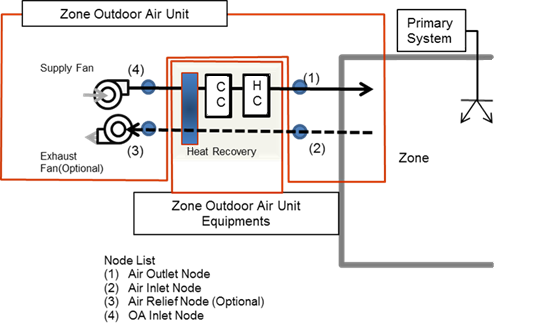
\includegraphics[width=0.9\textwidth, height=0.9\textheight, keepaspectratio=true]{media/image282.png}
\caption{Zone Outdoor Air Unit Schematic \protect \label{fig:zone-outdoor-air-unit-schematic}}
\end{figure}

When an AirloopHVAC serves the same zone, it is strongly recommended that the outdoor and exhaust air flow rates are balanced. In addition, the exhaust airflow rate and air schedule should be the same as outdoor air flow rate and outdoor air schedule, respectively. Otherwise, possible unbalanced flows will cause improper return airflow unless \hyperref[zoneairmassflowconservation]{ZoneAirMassFlowConservation} is active.

The full input for zone outdoor air units is described below using a variety of fields.

\subsubsection{Inputs}\label{inputs-5-035}

\paragraph{Field: Name}\label{field-name-5-029}

This field is simply the identifying name that distinguishes one particular outdoor air unit from another in the input data file. Like all other names in EnergyPlus, it is assumed that this is a unique character string and that no other zone outdoor air units use this same name.

\paragraph{Field: Availability Schedule Name}\label{field-availability-schedule-name-5-005}

This field is a schedule name (ref: Schedule) that determines whether the zone outdoor air unit is available to operate. A schedule value greater than 0 (usually 1 is used) indicates that the outdoor air unit can be on during the time period. A value less than or equal to 0 (usually 0 is used) denotes that the outdoor air unit must be off for the time period. If this field is blank, the schedule has values of 1 for all time periods. For any schedule value greater than zero, the outdoor air unit is considered available and will operate at the supply and exhaust flow rates defined by input field described below.

\paragraph{Field: Zone Name}\label{field-zone-name-016}

This field is the name of the zone (Ref: Zone) in which the outdoor air unit is located and intended to affect.~ Zone outdoor air units impact only a single zone.

\paragraph{Field: Outdoor Air Flow Rate}\label{field-outdoor-air-flow-rate}

This field allows the user to enter the volumetric flow rate of outdoor air (in m\(^{3}\)/sec) that will be brought in through the outdoor air unit. The actual outdoor air flow rate will be this number multiplied by the schedule value from the outdoor air schedule. This field is autosizable.~ When autosized, the unit's outdoor air flow rate will match the minimum outdoor air requirements specified through the \hyperref[sizingzone]{Sizing:Zone} object.

\paragraph{Field: Outdoor Air Schedule Name}\label{field-outdoor-air-schedule-name-1}

This field contains a schedule name (ref: Schedule) that contains values for modifying the outdoor air flow rate.~ The supply air flow rate is the product of the outdoor air flow rate and the outdoor air schedule value for the time of interest. ~Note that if the outdoor air unit is scheduled off that the system will not operate regardless of the outdoor air schedule value. However, if the system is operating, it will always bring in this fraction of the outdoor air flow rate.

\paragraph{Field: Supply Fan Name}\label{field-supply-fan-name-000}

This field is the name of a fan (ref: \hyperref[fansystemmodel]{Fan:SystemModel}, \hyperref[fanconstantvolume]{Fan:ConstantVolume}, \hyperref[fanvariablevolume]{Fan:VariableVolume}) that is part of the zone outdoor air unit. This name links the outdoor air unit to particular fan data entered elsewhere in the input data file. A fan name is required since it is the prime mover of air in the outdoor air control unit.

\paragraph{Field: Fan Placement}\label{field-fan-placement-1-001}

This field has two choices: \textbf{BlowThrough} or \textbf{DrawThrough}. The first choice stands for ``blow through fan''. It means that the unit consists of outdoor air node followed by a supply fan followed by the equipment that are part of the system. The second choice stands for ``draw through fan''. It means that the supply fan placed at the end of supply air stream and supply fan outlet node is identified with the air outlet node. The fan ``draws air through'' the equipment system.

\begin{itemize}
\item
  BlowThrough
\item
  DrawThrough
\end{itemize}

If the user does not select a fan placement type, \textbf{DrawThrough} is assumed as default by EnergyPlus.

\paragraph{Field: Exhaust Fan Name}\label{field-exhaust-fan-name}

This field is the name of a fan (ref: \hyperref[fansystemmodel]{Fan:SystemModel}, \hyperref[fanconstantvolume]{Fan:ConstantVolume}, \hyperref[fanvariablevolume]{Fan:VariableVolume}) that is part of the outdoor air unit. This name links the outdoor air unit to particular fan data entered elsewhere in the input data file. This field is optional.

\paragraph{Field: Exhaust Air Flow Rate}\label{field-exhaust-air-flow-rate}

This field allows the user to enter the volumetric flow rate of air (in m\(^{3}\)/sec) that will be exhausted to the outdoors. The actual exhaust air flow rate will be this number multiplied by the schedule value from the exhaust air schedule. If the exhaust fan name is left blank, this field will be ignored and automatically set to be equal to zero.

\paragraph{Field: Exhaust Air Schedule Name}\label{field-exhaust-air-schedule-name}

This field contains a schedule name (ref: Schedule) that should contain values for modifying the exhaust air flow rate.~ The actual exhaust air flow rate equals the exhaust air flow rate input (previous field) multiplied by the exhaust air schedule value. If the exhaust fan name is left blank, this field will be ignored and automatically set to be equal to zero.

\paragraph{Field: Unit Control Type}\label{field-unit-control-type}

The unit control type field determines with conditions in the zone being served what the response of the zone outdoor air system will be. It is important to note that this only controls the temperature of the air being delivered to the space not whether or not the system will operate.~ There are two options for this field: Neutral or Temperature. Neutral control tries to have no energy impact on the zone by delivering air at the temperature of the zone. This allows air to be delivered to the zone without affecting the zone air heat balance and thus provides outside air without impacting any other system providing conditioning to this zone. The temperature control option will supply air to the zone based on the high and low air control temperature schedules (see next two fields). For temperature control, when the outside air temperature is less than the low air control temperature, the zone outdoor air unit will provide whatever heating is available from its components to achieve the low air temperature value.~ When the outside air temperature is above the high air control temperature, the zone outdoor air unit will provide whatever cooling is available from its components to achieve the high air temperature value.~ When the outdoor air temperature is between the high and low air control temperatures, the unit will simply provide air at whatever the outdoor air conditions are, modified by any fan heat added by the supply fan. In summary, the user must select from the following two options:

\begin{itemize}
\item
  NeutralControl
\item
  TemperatureControl
\end{itemize}

If the user does not select a unit control type, \textbf{NeutralControl} is assumed as the default by EnergyPlus.

\paragraph{Field: High Air Control Temperature Schedule Name}\label{field-high-air-control-temperature-schedule-name}

This field specifies the dry-bulb air temperature in degrees Celsius for the supply air temperature to the zone. When the outdoor air temperature or post-supply fan outlet temperature in the case of blow through is above the high air control temperature, a cooling coil, if available and specified by the user, is tuned on to conditioning the outdoor air to the high control temperature. This field only applies to zone outdoor air units that use Temperature Control (see previous field).

\paragraph{Field: Low Air Control Temperature Schedule Name}\label{field-low-air-control-temperature-schedule-name}

This field specifies the dry-bulb air temperature in degrees Celsius for the supply air temperature to the zone. When the outdoor air temperature or post-supply fan outlet temperature is below the low air control temperature, a heating coil, if available and specified by the user, is tuned on to conditioning the outdoor air to the low control temperature. This field only applies to zone outdoor air units that use Temperature Control (see two previous fields).

\paragraph{Field: Outdoor Air Node Name}\label{field-outdoor-air-node-name-1-000}

This field is a node name used to identify the node associated with fresh air brought into the outdoor air unit from the outdoor environment. It should also be defined in an \hyperref[outdoorairnode]{OutdoorAir:Node} object with the same name and assigned an optional height (above ground).

\paragraph{Field: Air Outlet Node Name}\label{field-air-outlet-node-name-3-003}

This field is a node name used to identify the node that serves as the outlet (air side) from the zone outdoor air unit. In EnergyPlus, nodes represent points between components or at various points in the loops. In an outdoor air unit, the air outlet node from the system will typically be the same node as a zone inlet node. While a node name may be referenced more than once in an input data file, each node must have a unique name.

\paragraph{Field: Air Inlet Node Name}\label{field-air-inlet-node-name-3-003}

This field is a node name used to identify the node that serves as the inlet (air side) to the exhaust side of the outdoor air unit. In EnergyPlus, nodes represent points between components or at various points in the loops. In an outdoor air unit, the air inlet node of the system will typically be the same node as a zone outlet node. While a node name may be referenced more than once in an input data file, each node must have a unique name.

\paragraph{Field: Supply Fan Outlet Node Name}\label{field-supply-fan-outlet-node-name}

This field is a node name used to identify the node that serves as the outlet (air side) of the supply fan for the zone outdoor air unit. In EnergyPlus, nodes represent points between components or at various points in the loops. While a node name may be referenced more than once in an input data file, each node must have a unique name.

\paragraph{Field: Outdoor Air Unit List Name}\label{field-outdoor-air-unit-list-name}

This field is the name of an \hyperref[zonehvacoutdoorairunitequipmentlist]{ZoneHVAC:OutdoorAirUnit:EquipmentList} object. An \hyperref[zonehvacoutdoorairunitequipmentlist]{ZoneHVAC:OutdoorAirUnit:EquipmentList} ~is simply a list of components giving both component name and type. This equipment list specifies all the components that will be simulated in this unit. The order of the components in the list is significant: components are simulated sequentially in the order given in the Equipment List.

\paragraph{Field: Availability Manager List Name}\label{field-availability-manager-list-name-4}

This optional input field is the name of an \hyperref[availabilitymanagerassignmentlist]{AvailabilityManagerAssignmentList} object. An Availability Manager Assignment List is a list of Availability Managers giving both Availability Manager type and name. The availability managers in the list apply to this outdoor air unit~ object's fan. If the outdoor air unit is available (per the Availability Schedule Name input field above) and this input field has a valid availability manager assignment list name, then the availability managers in the list determine when and if the fan of this outdoor air unit~ object should be on or off.

An example of this object defined in an input data file is shown below\textbf{:}

\begin{lstlisting}

ZoneHVAC:OutdoorAirUnit,
      Zone5DXOutAir,           !- Name
      OAUnitOASched,           !- Availability Schedule Name
      SPACE5-1,                !- Zone Name
      0.42,                    !- Outdoor Air Flow Rate {m3/s}
      OAUnitOASched,           !- Outdoor Air Schedule Name
      Zone5OAUFan1,            !- Supply Fan Name
      BlowThrough,             !- Supply Fan Placement
      ,                        !- Exhaust Fan Name
      ,                        !- Exhaust Air Flow Rate {m3/s}
      ,                        !- Exhaust Air Schedule Name
      TemperatureControl,      !- Unit Control Type
      OAUHitemp2,              !- High Air Control Temperature Schedule Name
      OAULotemp2,              !- Low Air Control Temperature Schedule Name
      Zone5OAUOANode,          !- Outdoor Air Node Name
      Zone5OAUZoneInletNode,   !- AirOutlet Node Name
      Zone5OAUZoneOutletNode,  !- AirInlet Node Name
      Zone5OAUFanOutletNode,   !- Supply FanOutlet Node Name
      Zone5OAUEquip1;          !- Outdoor Air Unit List Name
\end{lstlisting}

\subsubsection{Outputs}\label{outputs-5-012}

\begin{itemize}
\item
  HVAC,Average, Zone Outdoor Air Unit Total Heating Rate {[}W{]}
\item
  HVAC,Sum, Zone Outdoor Air Unit Total Heating Energy {[}J{]}
\item
  HVAC,Average, Zone Outdoor Air Unit Total Cooling Rate {[}W{]}
\item
  HVAC,Sum, Zone Outdoor Air Unit Total Cooling Energy {[}J{]}
\item
  HVAC,Average, Zone Outdoor Air Unit Sensible Cooling Rate {[}W{]}
\item
  HVAC,Sum, Zone Outdoor Air Unit Sensible Heating Energy {[}J{]}
\item
  HVAC,Average, Zone Outdoor Air Unit Fan Electricity Rate {[}W{]}
\item
  HVAC,Sum, Zone Outdoor Air Unit Fan Electricity Energy {[}J{]}
\item
  HVAC,Average, Zone Outdoor Air Unit Air Mass Flow Rate {[}kg/s{]}
\item
  HVAC,Average, Zone Outdoor Air Unit Fan Availability Status {[]}
\item
  Zone Outdoor Air Unit Latent Cooling Energy
\end{itemize}

\paragraph{Zone Outdoor Air Unit Total Heating Rate {[}W{]}}\label{zone-outdoor-air-unit-total-heating-rate-w}

This field reports the heating output rate of the outdoor air unit system to the zone it is serving in Watts. This is determined by outlet and zone air conditions and the mass flow rate through the zone outdoor air unit.

\paragraph{Zone Outdoor Air Unit Total Heating Energy {[}J{]}}\label{zone-outdoor-air-unit-total-heating-energy-j}

This field is the heating output of the outdoor air unit system to the zone it is serving in Joules over the timestep being reported. This is determined by outlet and zone air conditions, the mass flow rate through the zone outdoor air unit, and the time step.

\paragraph{Zone Outdoor Air Unit Total Cooling Rate {[}W{]}}\label{zone-outdoor-air-unit-total-cooling-rate-w}

This field reports the total cooling (sensible plus latent) output rate of the outdoor air unit system to the zone it is serving in Watts. This is determined by outlet and zone air conditions and the mass flow rate through the zone outdoor air unit.

\paragraph{Zone Outdoor Air Unit Total Cooling Energy {[}J{]}}\label{zone-outdoor-air-unit-total-cooling-energy-j}

This field is the total cooling (sensible plus latent) output of the outdoor air unit system to the zone it is serving in Joules over the timestep being reported. This is determined by outlet and zone air conditions, the mass flow rate through the zone outdoor air unit, and the time step.

\paragraph{Zone Outdoor Air Unit Sensible Cooling Energy {[}J{]}}\label{zone-outdoor-air-unit-sensible-cooling-energy-j}

\paragraph{Zone Outdoor Air Unit Sensible Cooling Rate {[}W{]}}\label{zone-outdoor-air-unit-sensible-cooling-rate-w}

These reports are the sensible cooling output rate of the outdoor air unit system to the zone it is serving in Joules or Watts. This is determined by outlet and zone air conditions and the mass flow rate through the zone outdoor air unit.

\paragraph{Zone Outdoor Air Unit Sensible Heating Energy {[}J{]}}\label{zone-outdoor-air-unit-sensible-heating-energy-j}

\paragraph{Zone Outdoor Air Unit Sensible Heating Rate {[}W{]}}\label{zone-outdoor-air-unit-sensible-heating-rate-w}

These are the sensible heating output of the outdoor air unit system to the zone it is serving in Joules or Watts over the timestep being reported. This is determined by outlet and zone air conditions, the mass flow rate through the zone outdoor air unit, and the time step.

\paragraph{Zone Outdoor Air Unit Latent Cooling Energy {[}J{]}}\label{zone-outdoor-air-unit-latent-cooling-energy-j}

\paragraph{Zone Outdoor Air Unit Latent Cooling Rate {[}W{]}}\label{zone-outdoor-air-unit-latent-cooling-rate-w}

These are the latent cooling output of the outdoor air unit system to the zone it is serving, in Joules and Watts. This is determined by outlet and zone air conditions, the mass flow rate through the zone outdoor air unit, and the time step.

\paragraph{Zone Outdoor Air Unit Latent Heating Energy {[}J{]}}\label{zone-outdoor-air-unit-latent-heating-energy-j}

\paragraph{Zone Outdoor Air Unit Latent Heating Rate {[}W{]}}\label{zone-outdoor-air-unit-latent-heating-rate-w}

These are the latent heating output of the outdoor air unit system to the zone it is serving, in Joules and Watts. This is determined by outlet and zone air conditions, the mass flow rate through the zone outdoor air unit, and the time step.

\paragraph{Zone Outdoor Air Unit Fan Electricity Rate {[}W{]}}\label{zone-outdoor-air-unit-fan-electric-power-w}

This field reports the electric power consumption rate of the fan of the outdoor air unit in Watts.

\paragraph{Zone Outdoor Air Unit Fan Electricity Energy {[}J{]}}\label{zone-outdoor-air-unit-fan-electric-energy-j}

This field reports the electric power consumed by the fan of the outdoor air unit over the time step in Joules.

\paragraph{Zone Outdoor Air Unit Air Mass Flow Rate {[}kg/s{]}}\label{zone-outdoor-air-unit-air-mass-flow-rate-kgs}

This field reports the air mass flow rate of the zone outdoor air unit Outdoor Air Unit~ in kilograms per second.

\paragraph{Zone Outdoor Air Unit Fan Availability Status {[]}}\label{zone-outdoor-air-unit-fan-availability-status}

This is the availability status of the outdoor air unit fan. This status flag is a result of the calculations made by the Availability Manager(s) listed in an AvailabilityManagerAssignmentList object and/or calculations made by Hybrid Ventilation Manager object. The AvailabilityManagerAssignmentList is an optional input in the outdoor air unit~ object. When a single availability manager is used in an Availability Manager Assignment List, this is also the availability status reported by the specific availability manager (Ref. AvailabilityManager:* Outputs). For multiple availability managers in an Availability Manager Assignment List (with or without Hybrid Ventilation Manager), rules to determine fan availability status are described in the section `Group -- System Availability Managers'. The control status outputs are represented using integers 0 through 3. These integers represent NoAction (0), ForceOff (1), CycleOn (2), and CycleOnZoneFansOnly (3). Since the status output is averaged, the output result may not correspond to the values described here when output variable frequencies other than detailed are used. Use the ``detailed'' reporting frequency (Ref. Output:Variable object) to view the availability status at each simulation timestep.

\subsection{ZoneHVAC:OutdoorAirUnit:EquipmentList}\label{zonehvacoutdoorairunitequipmentlist}

This input syntax is used to specify the components in a zone outdoor air unit. The components will be simulated in the order in which they occur in this list.

\subsubsection{Inputs}\label{inputs-6-032}

\paragraph{Field: Name}\label{field-name-6-027}

The user designated unique name of an instance of a zone outdoor air unit equipment list.

\paragraph{Field Set (Component Object Type, Component Name, Control Node Name) up to 8}\label{field-set-component-object-type-component-name-control-node-name-up-to-8}

After the identifying name, the list consists of up to 8 pairs of data items.

\paragraph{Field: Component \textless{}x\textgreater{} Object Type}\label{field-component-x-object-type-000}

This field specifies the keyword for the type of component used.

\paragraph{Field: Component \textless{}x\textgreater{} Name}\label{field-component-x-name-000}

This field is the unique name of the component specified in the previous field. This named object must appear in the IDF.

Note: If any of the components use the autosized option at the component level, input data for zone sizing purposes are required for the proper sizing of the components. Please refer to the~\hyperref[sizingzone]{Sizing:Zone}~object for more information.

An example from an IDF:

\begin{lstlisting}

ZoneHVAC:OutdoorAirUnit:EquipmentList,
      Zone5OAUEquip1,          !- Name
      Dehumidifier:Desiccant:NoFans,  !- Component 1 Object Type
      Z5Dessicant,             !- Component 1 Name
      HeatExchanger:AirToAir:FlatPlate,  !- Component 2 Object Type
      Zone5A2AHeat Recovery,   !- Component 2 Name
      CoilSystem:Cooling:DX,  !- Component 3 Object Type
      DX Cooling Coil System 5,!- Component 3 Name
      Coil:Heating:Electric,   !- Component 4 Object Type
      Zone5DESHCoil;           !- Component 4 Name
\end{lstlisting}

\subsection{ZoneHVAC:WindowAirConditioner}\label{zonehvacwindowairconditioner}

The Window Air Conditioner is a unit of zone equipment made up of other components. Each window air conditioner consists of an outdoor air mixer, a fan, and a direct expansion (DX) cooling coil. These components are described elsewhere in this document. The input for a window air conditioner requires the names of these three pieces of equipment, which are then specified individually elsewhere in the input. The input for a window air conditioner also requires the name of an availability schedule, the maximum unit airflow rate, and the maximum outdoor airflow rate for the unit. The unit is connected to a zone by specifying an air inlet node, which must be the same as a zone exhaust node; and an air outlet node, which must be the same as a zone inlet node (ref. \hyperref[zonehvacequipmentconnections]{ZoneHVAC:EquipmentConnections}).

A supply air fan operating mode schedule must also be specified. The supply air fan operating mode schedule value determines if the supply air fan can run continuously with the DX coil cycling on/off to match the zone cooling demand or the fan and DX coil can cycle on/off together to meet the cooling demand. The placement of the supply air fan, in relation to the DX coil, must also be specified (blow through or draw through). The cooling convergence tolerance is required, which is the tolerance denoting how closely the window air conditioner will meet the cooling load. The tolerance is always relative to the zone load (i.e., the unit will operate to meet the zone load to within the tolerance value times the zone load for each simulation timestep). Finally, the DX cooling coil type must be specified.

\subsubsection{Inputs}\label{inputs-7-031}

\paragraph{Field: Name}\label{field-name-7-025}

A unique user assigned name for an instance of a window air conditioner unit. Any reference to this window air conditioner by another object will use this name.

\paragraph{Field: Availability Schedule Name}\label{field-availability-schedule-name-6-005}

The name of the schedule (ref: Schedule) that denotes whether the window air conditioner unit can run during a given time period. A schedule value greater than 0 (usually 1 is used) indicates that the unit can be on during the time period. A value less than or equal to 0 (usually 0 is used) denotes that the unit must be off for the time period. If this field is blank, the schedule has values of 1 for all time periods.

\paragraph{Field: Maximum Supply Air Flow Rate}\label{field-maximum-supply-air-flow-rate-3}

The maximum volumetric airflow rate through the window air conditioner in cubic meters per second. Since the unit operates by cycling on/off, this is also the design, rated airflow rate of the unit.

\paragraph{Field: Maximum Outdoor Air Flow Rate}\label{field-maximum-outdoor-air-flow-rate-2-000}

If the window air conditioner uses outdoor air, this field specifies the outdoor air volumetric flow rate in cubic meters per second. This flow rate should be less than or equal to the maximum airflow rate. A value of zero specifies no outdoor air. Note that the outdoor airflow rate is fixed: it cannot change during the simulation

\paragraph{Field: Air Inlet Node Name}\label{field-air-inlet-node-name-4-002}

The name of the HVAC system node (see Node) from which the window air conditioner draws its indoor air. This should be one of the zone exhaust nodes for the zone which the window air conditioner is cooling.

\paragraph{Field: Air Outlet Node Name}\label{field-air-outlet-node-name-4-002}

The name of the HVAC system node (see Node) to which the window air conditioner sends its outlet air. This should be one of the inlet air nodes for the zone which is being cooled.

\paragraph{Field: Outdoor Air Mixer Object Type}\label{field-outdoor-air-mixer-object-type-1}

This field specifies the type of outdoor air mixer used by this window air conditioner unit. The outdoor air mixer component is part of the window air conditioner compound object. The only available outdoor air mixer type is:

\hyperref[outdoorairmixer]{OutdoorAir:Mixer}

\paragraph{Field: Outdoor Air Mixer Name}\label{field-outdoor-air-mixer-name-1}

The name of an outdoor air mixer component which composes part of the window air conditioner unit. Note that the return air node of the outdoor air mixer should be the same node as the air inlet node of the window air conditioner. In addition, the outdoor air mixer's mixed air node should be the same as the window air conditioner's fan inlet air node (for blow through) or the air conditioner's DX coil inlet node (for draw through)

\paragraph{Field: Supply Air Fan Object Type}\label{field-supply-air-fan-object-type-4}

This field specifies the type of supply air fan used by window air conditioner. The supply air fan is part of the window air conditioner compound object. The only valid supply air fan types are:

\begin{itemize}
\item
  \hyperref[fansystemmodel]{Fan:SystemModel}
\item
  \hyperref[fanonoff]{Fan:OnOff}
\item
  \hyperref[fanconstantvolume]{Fan:ConstantVolume}
\end{itemize}

Note that \hyperref[fansystemmodel]{Fan:SystemModel} was added as of version 8.7 and is recommended for use in new models.  \hyperref[fanonoff]{Fan:OnOff} and \hyperref[fanconstantvolume]{Fan:ConstantVolume}may be deprecated in a future version.

\paragraph{Field:Supply Air Fan Name}\label{fieldsupply-air-fan-name}

The name of the fan component that composes part of the window air conditioner. Note that the fan's maximum flow rate should be the same as the maximum airflow rate of the window air conditioner. A fan of type \hyperref[fansystemmodel]{Fan:SystemModel} or \hyperref[fanonoff]{Fan:OnOff} may be used with either cycling or continuous fan, and a fan of type \hyperref[fanconstantvolume]{Fan:ConstantVolume} is used only with continuous fan (see Supply Air Fan Operating Mode Schedule field below). The fan's inlet node should be the same as the outdoor air mixer's mixed air node (for blow through) or the DX coil's outlet node (for draw through). The fan's outlet node should be the same as the DX coil's air inlet node (for blow through) or the window air conditioner's air outlet node (for draw through).

\paragraph{Field: Cooling Coil Object Type}\label{field-cooling-coil-object-type-2-001}

This field specifies the type of cooling coil to be modeled for this window air conditioner. The input requirements for these cooling coil objects are described elsewhere in this document. If the user wants to control the enhanced dehumidification performance of the Heat Exchanger Assisted coil type based on zone air humidity level, then the input file must include a humidistat object (ref. \hyperref[zonecontrolhumidistat]{ZoneControl:Humidistat}) for the zone being served by this air conditioner and a high humidity set point manager (ref. \hyperref[setpointmanagersinglezonehumiditymaximum]{SetpointManager:SingleZone:Humidity:Maximum}) with the high humidity set point placed on the outlet node of the heat exchanger assisted cooling coil. Only allowable coil types are:

\begin{itemize}
\item
  \hyperref[coilcoolingdxsinglespeed]{Coil:Cooling:DX:SingleSpeed}
\item
  \hyperref[coilcoolingdxvariablespeed]{Coil:Cooling:DX:VariableSpeed}
\item
  \hyperref[coilsystemcoolingdxheatexchangerassisted]{CoilSystem:Cooling:DX:HeatExchangerAssisted}
\end{itemize}

\paragraph{Field: DX Cooling Coil Name}\label{field-dx-cooling-coil-name}

The name of a DX cooling coil component that composes part of the window air conditioner unit. The DX coil air inlet node should be the same as the fan outlet node (for blow through) or the outdoor air mixer's mixed air node (for draw through). The DX coil air outlet node should be the same as the window air conditioner's air outlet node (for blow through) or the fan's inlet node (for draw through).

\paragraph{Field: Supply Air Fan Operating Mode Schedule Name}\label{field-supply-air-fan-operating-mode-schedule-name-3-000}

This alpha field specifies the name of the supply air fan operating mode schedule. The supply air fan operating mode may vary during the simulation based on time-of-day or with a change of season. Schedule values of 0 denote that the supply air fan and the heating or cooling coil cycle on and off together to meet the heating or cooling load (a.k.a. AUTO fan). Schedule values other than 0 denote that the supply air fan runs continuously while the heating or cooling coil cycles to meet the load. If this field is left blank, the model assumes the supply air fan cycles with the heating or cooling coil throughout the simulation.

\paragraph{Field: Fan Placement}\label{field-fan-placement-2-000}

This input field has two choices: \textbf{BlowThrough} or \textbf{DrawThrough}. The first choice stands for ``blow through fan''. This means that the unit consists of an outdoor air mixer followed by a fan followed by a DX coil. The fan ``blows through'' the DX coil. The second choice stands for ``draw through fan''. This means that the unit consists of an outdoor air mixer followed by a DX coil followed by a fan. The fan ``draws air through'' the coil.

\paragraph{Field: Cooling Convergence Tolerance}\label{field-cooling-convergence-tolerance-2}

This input field defines the convergence tolerance for the unit's cooling output. This field allows the user some control over how closely the air conditioner will control the air-side conditions. The relative size of this parameter relates directly to the closeness of the control. A very small value in this field will result in tight control and will probably result in larger numbers of iterations. A large value in this field will result in looser controls and could result in unsatisfactory fluctuations in zone air temperature. Initial experience with this parameter lends to the recommendation of using 0.001 as the starting point.

The window air conditioner is controlled by matching its sensible (temperature) cooling output to the zone sensible load (demand). Because the performance of the DX coil is frequently non-linear, the air conditioner model must call the DX coil model several times (iterate) to determine the proper run time fraction to meet the zone load. The cooling convergence tolerance is the error tolerance used to terminate the iteration procedure when the following equation is satisfied:

\begin{equation}
\frac{{\left| {{Q_{ZoneLoad}} - {Q_{WindowAirConditioner,out}})} \right|}}{{{Q_{ZoneLoad}}}} \le Cooling{\kern 1pt} Convergence{\kern 1pt} Tolerance
\end{equation}

The maximum number of iterations is limited, with a warning message generated if the above equation is not satisfied within the maximum number of iterations.

\paragraph{Field: Availability Manager List Name}\label{field-availability-manager-list-name-5}

This optional input field is the name of an \hyperref[availabilitymanagerassignmentlist]{AvailabilityManagerAssignmentList} object. An Availability Manager Assignment List is a list of Availability Managers giving both Availability Manager type and name. The availability managers in the list apply to this window air conditioner or object's fan. If the window air conditioner is available (per the Availability Schedule Name input field above) and this input field has a valid availability manager assignment list name, then the availability managers in the list determine when and if the fan of this window air conditioner object should be on or off.

\paragraph{Field: Design Specification ZoneHVAC Sizing Object Name}\label{field-design-specification-zonehvac-sizing-object-name-5}

This optional input field is the name of a \hyperref[designspecificationzonehvacsizing]{DesignSpecification:ZoneHVAC:Sizing} object. The name must correspond to unique name of a \hyperref[designspecificationzonehvacsizing]{DesignSpecification:ZoneHVAC:Sizing} object. A Design Sepcification Zone HVAC Sizing object defines scalable sizing methods for sizing input fields such as Maximum Air Flow Rate in this Window Air Conditioner zone HVAC object. The scaled Maximum Air Flow Rate in turn is used to size cooling capacity of the unit.

Following is an example input for the cycling window air conditioner, along with its constituent components.

\begin{lstlisting}

  ZoneHVAC:WindowAirConditioner,
         Zone3WindAC,                  ! name of window AC unit
         FanAndCoilAvailSched,         ! Availability Schedule Name
         0.6,                          ! Maximum Supply Air Flow Rate {m3/s}
         0.05,                         ! Maximum Outdoor Air Flow Rate {m3/s}
         Zone3WindACAirInletNode,      ! Air Inlet Node Name
         Zone3WindACAirOutletNode,     ! Air Outlet Node Name
         OutdoorAir:Mixer,             ! Outdoor Air Mixer Object Type
         Zone3WindACOAMixer,           ! Outdoor Air Mixer Name
         Fan:SystemModel,              ! Supply Air Fan Object Type
         Zone3WindACFan,               ! Fan Name
         Zone3WindACDXCoil,            ! DX Cooling Coil Name
         CyclingFanSch,                ! Supply Air Fan Operation Mode Schedule Name
         DrawThrough,                  ! Fan Placement
         0.001,                        ! Cooling Convergence Tolerance
         Coil:Cooling:DX:SingleSpeed;  ! Cooling Coil Object Type

  Schedule:Compact,
         CyclingFanSch,                !- Name
         Fraction,                     !- ScheduleType
         Through: 12/31,               !- Complex Field \#1
         For: AllDays,                 !- Complex Field \#2
         Until: 24:00,                 !- Complex Field \#7
         0.0;                          !- Complex Field \#8

  OutdoorAir:Mixer,
         Zone3WindACOAMixer,           ! Name
         Zone3WindACOAMixerOutletNode, ! Mixed Air Node Name
         Zone3WindACOAInNode,          ! Outdoor Air Stream Node Name
         Zone3WindACExhNode,           ! Relief Air Stream Node Name
         Zone3WindACAirInletNode;      ! Return Air Stream Node Name

  Fan:SystemModel,
       Zone3WindACFan ,                !- Name
       FanAndCoilAvailSched ,          !- Availability Schedule Name
       Zone3WindACDXOutletNode,        !- Air Inlet Node Name
       Zone3WindACAirOutletNode,       !- Air Outlet Node Name
       0.6 ,                           !- Design Maximum Air Flow Rate
       Discrete ,                      !- Speed Control Method
       0.0,                            !- Electric Power Minimum Flow Rate Fraction
       75.0,                           !- Design Pressure Rise
       0.9 ,                           !- Motor Efficiency
       1.0 ,                           !- Motor In Air Stream Fraction
       AUTOSIZE,                       !- Design Electric Power Consumption
       TotalEfficiencyAndPressure,     !- Design Power Sizing Method
       ,                               !- Electric Power Per Unit Flow Rate
       ,                               !- Electric Power Per Unit Flow Rate Per Unit Pressure
       0.5;                            !- Fan Total Efficiency

  Coil:Cooling:DX:SingleSpeed,
      Zone3WindACDXCoil,       !- Name
      CoolingCoilAvailSched,   !- Availability Schedule Name
      autosize,                !- Rated Total Cooling Capacity {W}
      autosize,                !- Rated Sensible Heat Ratio
      3.0,                     !- Rated COP
      autosize,                !- Rated Air Flow Rate {m3/s}
      Zone3WindACOAMixerOutletNode,  !- Air Inlet Node Name
      Zone3WindACDXOutletNode, !- Air Outlet Node Name
      WindACCoolCapFT,         !- Total Cooling Capacity Function of Temperature Curve Name
      WindACCoolCapFFF,        !- Total Cooling Capacity Function of Flow Fraction Curve Name
      WindACEIRFT,             !- Energy Input Ratio Function of Temperature Curve Name
      WindACEIRFFF,            !- Energy Input Ratio Function of Flow Fraction Curve Name
      WindACPLFFPLR;           !- Part Load Fraction Correlation Curve Name
\end{lstlisting}

\subsubsection{Outputs}\label{outputs-6-012}

\begin{itemize}
\item
  HVAC,Average,Zone Window Air Conditioner Total Cooling Rate {[}W{]}
\item
  HVAC,Sum,Zone Window Air Conditioner Total Cooling Energy {[}J{]}
\item
  HVAC,Average,Zone Window Air Conditioner Sensible Cooling Rate {[}W{]}
\item
  HVAC,Sum,Zone Window Air Conditioner Sensible Cooling Energy {[}J{]}
\item
  HVAC,Average,Zone Window Air Conditioner Latent Cooling Rate {[}W{]}
\item
  HVAC,Sum,Zone Window Air Conditioner Latent Cooling Energy {[}J{]}
\item
  HVAC,Average,Zone Window Air Conditioner Electricity Rate {[}W{]}
\item
  HVAC,Sum,Zone Window Air Conditioner Electricity Energy {[}J{]}
\item
  HVAC,Average, Zone Window Air Conditioner Fan Part Load Ratio {[]}
\item
  HVAC,Average, Zone Window Air Conditioner Compressor Part Load Ratio {[]}
\item
  HVAC,Average,Zone Window Air Conditioner Fan Availability Status {[]}
\end{itemize}

\paragraph{Zone Window Air Conditioner Total Cooling Rate {[}W{]}}\label{zone-window-air-conditioner-total-cooling-rate-w}

This field is the total (sensible and latent) heat extraction rate of the window air conditioner unit from the zone it is serving in Watts. This is determined by the outlet and zone conditions and the mass flow rate through the unit.

\paragraph{Zone Window Air Conditioner Total Cooling Energy {[}J{]}}\label{zone-window-air-conditioner-total-cooling-energy-j}

This is the total (sensible and latent) heat extraction of the window air conditioner unit from the zone it is serving in Joules over the timestep being reported. This is determined by outlet and zone air conditions, the mass flow rate through the unit, and the timestep.

\paragraph{Zone Window Air Conditioner Sensible Cooling Rate {[}W{]}}\label{zone-window-air-conditioner-sensible-cooling-rate-w}

This field reports the moist air sensible heat extraction rate of the window air conditioner unit from the zone it is serving in Watts. This is determined by the outlet and zone conditions and the mass flow rate through the unit.

\paragraph{Zone Window Air Conditioner Sensible Cooling Energy {[}J{]}}\label{zone-window-air-conditioner-sensible-cooling-energy-j}

This field reports the moist air sensible heat extraction of the window air conditioner unit from the zone it is serving in Joules over the timestep being reported. This is determined by the outlet and zone conditions and the mass flow rate through the unit.

\paragraph{Zone Window Air Conditioner Latent Cooling Rate {[}W{]}}\label{zone-window-air-conditioner-latent-cooling-rate-w}

This output is the latent heat extraction rate of the window air conditioner unit from the zone it is serving in Watts. This is determined by the outlet and zone conditions and the mass flow rate through the unit.

\paragraph{Zone Window Air Conditioner Latent Cooling Energy {[}J{]}}\label{zone-window-air-conditioner-latent-cooling-energy-j}

This is the latent heat extraction of the window air conditioner unit from the zone it is serving in Joules over the timestep being reported. This is determined by the outlet and zone conditions and the mass flow rate through the unit.

\paragraph{Zone Window Air Conditioner Electricity Rate {[}W{]}}\label{zone-window-air-conditioner-electric-powerw}

This output is the electricity consumption rate of the window air conditioner unit in Watts. The consumption includes electricity used by the compressor and the fans (indoor supply air fan and the condenser fan).

\paragraph{Zone Window Air Conditioner Electricity Energy {[}J{]}}\label{zone-window-air-conditioner-electric-energy-j}

This output is the electricity consumption of the window air conditioner unit in Joules for the time period being reported. The consumption includes electricity used by the compressor and the fans (indoor supply air fan and the condenser fan).

\paragraph{Zone Window Air Conditioner Fan Part Load Ratio {[]}}\label{zone-window-air-conditioner-fan-part-load-ratio}

This is the fan's part load ratio for the report timestep during which the fan had operated.

\paragraph{Zone Window Air Conditioner Compressor Part Load Ratio {[]}}\label{zone-window-air-conditioner-compressor-part-load-ratio}

This is the part load ratio of the report timestep during which the DX unit compressor had operated.

\textbf{\emph{Zone Window Air Conditioner Fan Availability Status {[]}}}

This is the availability status of the window air conditioner fan. This status flag is a result of the calculations made by the Availability Manager(s) listed in an AvailabilityManagerAssignmentList object and/or calculations made by Hybrid Ventilation Manager object. The AvailabilityManagerAssignmentList is an optional input in the window air conditioner object. When a single availability manager is used in an Availability Manager Assignment List, this is also the availability status reported by the specific availability manager (Ref. AvailabilityManager:* Outputs). For multiple availability managers in an Availability Manager Assignment List (with or without Hybrid Ventilation Manager), rules to determine fan availability status are described in the section `Group -- System Availability Managers'. The control status outputs are represented using integers 0 through 3. These integers represent NoAction (0), ForceOff (1), CycleOn (2), and CycleOnZoneFansOnly (3). Since the status output is averaged, the output result may not correspond to the values described here when output variable frequencies other than detailed are used. Use the ``detailed'' reporting frequency (Ref. Output:Variable object) to view the availability status at each simulation timestep.

\subsection{ZoneHVAC:PackagedTerminalAirConditioner}\label{zonehvacpackagedterminalairconditioner}

The packaged terminal air conditioner (PTAC) is a compound object made up of other components. Each PTAC consists of an outdoor air mixer, direct expansion (DX) cooling coil, heating coil (gas, electric, hot water, or steam) and a supply air fan. While the figure below shows the PTAC with draw through fan placement, blow through fan placement can also be modeled by positioning the supply air fan between the outdoor air mixer and the DX cooling coil. The packaged terminal air conditioner coordinates the operation of these components and is modeled as a type of zone equipment (Ref. \hyperref[zonehvacequipmentlist]{ZoneHVAC:EquipmentList} and \hyperref[zonehvacequipmentconnections]{ZoneHVAC:EquipmentConnections}).

\begin{figure}[hbtp] % fig 111
\centering
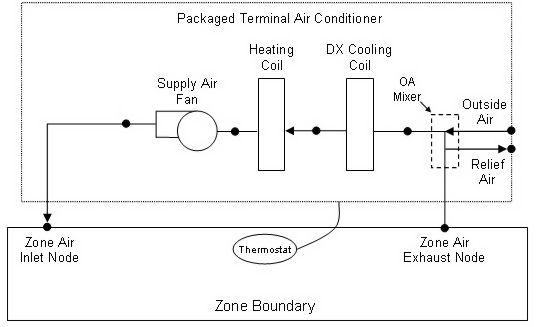
\includegraphics[width=0.9\textwidth, height=0.9\textheight, keepaspectratio=true]{media/image284.png}
\caption{  Schematic of a packaged terminal air conditioner with draw through fan placement \protect \label{fig:schematic-of-a-packaged-terminal-air-001}}
\end{figure}

Links to the PTAC's supply air fan, DX cooling coil, heating coil, and outdoor air mixer specifications are provided in the air conditioner's input syntax. Additional inputs include supply and outdoor air flow rates during cooling operation, heating operation, and when neither cooling or heating is required. A description of each input field for the packaged terminal air conditioner compound object is provided below.

\subsubsection{Inputs}\label{inputs-8-029}

\paragraph{Field: Name}\label{field-name-8-025}

This alpha field defines a unique user-assigned name for an instance of a packaged terminal air conditioner. Any reference to this air conditioner by another object will use this name.

\paragraph{Field: Availability Schedule Name}\label{field-availability-schedule-name-7-005}

This alpha field defines the name of the schedule (ref: Schedule) that denotes whether the air conditioner operates during a given time period. A schedule value equal to 0 denotes that the air conditioner must be off for that time period. A value greater than 0 denotes that the air conditioner is available to operate during that time period. This schedule may be used to completely disable the air conditioner (all of its coils and the supply air fan) as required. If this field is blank, the schedule has values of 1 for all time periods.

\paragraph{Field: Air Inlet Node Name}\label{field-air-inlet-node-name-5-001}

This alpha field defines the name of the HVAC system node from which the air conditioner draws its inlet air. This node name must be the name of a zone air exhaust node (Ref. \hyperref[zonehvacequipmentconnections]{ZoneHVAC:EquipmentConnections}).

\paragraph{Field: Air Outlet Node Name}\label{field-air-outlet-node-name-5-001}

This alpha field defines the name of the HVAC system node to which the air conditioner sends its outlet air. This node name must be the name of a zone air inlet node (Ref. \hyperref[zonehvacequipmentconnections]{ZoneHVAC:EquipmentConnections}).

\paragraph{Field: Outdoor Air Mixer Object Type}\label{field-outdoor-air-mixer-object-type-2}

This field specifies the type of outdoor air mixer used by this PTAC. The outdoor air mixer component is part of the PTAC unit. The only available outdoor air mixer type is:

\begin{itemize}
\tightlist
\item
  \hyperref[outdoorairmixer]{OutdoorAir:Mixer}
\end{itemize}

This input field should be left blank when the PTAC is connected to an \textit{\hyperref[airterminalsingleductmixer]{AirTerminal:SingleDuct:Mixer}} object. If this field is left blank, an outdoor air mixer object is not simulated.

\paragraph{Field: Outdoor Air Mixer Name}\label{field-outdoor-air-mixer-name-2}

This alpha field defines the name of an outdoor air mixer component which composes part of the PTAC. The return air node of the outdoor air mixer should also be the same node as the air inlet node of the PTAC. Furthermore, the outdoor air mixer's mixed air node should be the same as the PTAC's fan inlet air node (for blow through fan placement) or the PTAC's DX cooling coil inlet node (for draw through fan placement). This field should be left blank when the PTAC is connected to an \textit{\hyperref[airterminalsingleductmixer]{AirTerminal:SingleDuct:Mixer}} object.

\paragraph{Field: Cooling Supply Air Flow Rate}\label{field-cooling-supply-air-flow-rate-002}

This numeric field defines the supply air flow rate leaving the air conditioner in cubic meters per second when the DX cooling coil is operating. Values must be greater than 0 or this field is autosizable.

\paragraph{Field: Heating Supply Air Flow Rate}\label{field-heating-supply-air-flow-rate-002}

This numeric field defines the supply air flow rate leaving the air conditioner in cubic meters per second when the heating coil is operating. Values must be greater than 0 or this field is autosizable.

\paragraph{Field: No Load Supply Air Flow Rate}\label{field-no-load-supply-air-flow-rate-001}

This numeric field defines the supply air flow rate leaving the air conditioner in cubic meters per second when neither cooling nor heating is required (i.e., DX coil and heater are off but the supply air fan operates). This field is only used when the air conditioner's supply air fan operating mode schedule specifies continuous fan operation. Values must be greater than or equal to zero, or this field is autosizable. If the air conditioner's supply air fan operating mode schedule specifies continuous fan operation and this value is set to zero or this field is left blank, then the model assumes that the supply air flow rate when no cooling/heating is needed is equal to the supply air flow rate when the cooling or heating coil was last operating (for cooling operation or heating operation).

\paragraph{Field: Cooling Outdoor Air Flow Rate}\label{field-cooling-outdoor-air-flow-rate-001}

This numeric field defines the outdoor air flow rate through the air conditioner in cubic meters per second when the DX cooling coil is operating. Values must be greater than or equal to 0, or this field is autosizable. Note that the Cooling Outdoor Air Flow Rate is fixed; it cannot change during the simulation. In addition, the Cooling Outdoor Air Flow Rate cannot be greater than the air conditioner's supply air volumetric flow rate during cooling operation. This field is set to zero flow when the PTAC is connected to an \textit{\hyperref[airterminalsingleductmixer]{AirTerminal:SingleDuct:Mixer}} object.

\paragraph{Field: Heating Outdoor Air Flow Rate}\label{field-heating-outdoor-air-flow-rate-001}

This numeric field defines the outdoor air flow rate through the air conditioner in cubic meters per second when the heating coil is operating. Values must be greater than or equal to 0, or this field is autosizable. Note that the Heating Outdoor Air Flow Rate is fixed; it cannot change during the simulation. In addition, the Heating Outdoor Air Flow Rate cannot be greater than the air conditioner's supply air volumetric flow rate during heating operation. This field is set to zero flow when the PTAC is connected to an \textit{\hyperref[airterminalsingleductmixer]{AirTerminal:SingleDuct:Mixer}} object.

\paragraph{Field: No Load Outdoor Air Flow Rate}\label{field-no-load-outdoor-air-flow-rate-000}

This numeric field defines the outdoor air flow rate through the air conditioner in cubic meters per second when neither cooling nor heating is required (i.e., cooling and heating coils are off but the supply air fan operates). Values must be greater than or equal to 0, or this field is autosizable. Note that the outdoor air flow rate when no cooling/heating is needed is fixed; it cannot change during the simulation. In addition, the outdoor air flow rate when no cooling/heating is needed cannot be greater than the air conditioner's supply air volumetric flow rate when no cooling/heating is needed. This field is only used when the air conditioner's supply air fan operating mode schedule specifies continuous fan operation. If the air conditioner's supply air fan operating mode schedule specifies continuous fan operation and the field `Supply air volumetric flow rate when no cooling or heating is needed' is set to zero or is left blank, then the model assumes that the outdoor air flow rate when no cooling/heating is needed is equal to the outdoor air flow rate when the cooling or heating coil was last operating (for cooling operation {[}i.e., Cooling Outdoor Air Flow Rate{]} or heating operation {[}i.e., Heating Outdoor Air Flow Rate{]}) and this field is not used. This input field is set to zero flow when the PTAC is connected to an \textit{\hyperref[airterminalsingleductmixer]{AirTerminal:SingleDuct:Mixer}} object.

\paragraph{Field: Supply Air Fan Object Type}\label{field-supply-air-fan-object-type-5}

This alpha field defines the type of fan used by this PTAC. The only valid choices are \textbf{\hyperref[fansystemmodel]{Fan:SystemModel}}, \textbf{\hyperref[fanonoff]{Fan:OnOff}}, and \textbf{\hyperref[fanconstantvolume]{Fan:ConstantVolume}}. A fan of type \hyperref[fansystemmodel]{Fan:SystemModel} or \hyperref[fanonoff]{Fan:OnOff} is used with cycling fan operating mode, and a fan of type \hyperref[fansystemmodel]{Fan:SystemModel} or \hyperref[fanconstantvolume]{Fan:ConstantVolume} is used with continuous fan operating mode (see Supply Air Fan Operating Mode Schedule field below). The input requirements for these fan objects are described elsewhere in this document. Note that \hyperref[fansystemmodel]{Fan:SystemModel} was added as of version 8.7 and is recommended for use in new models.  \hyperref[fanonoff]{Fan:OnOff} and \hyperref[fanconstantvolume]{Fan:ConstantVolume} may be deprecated in a future version.

\paragraph{Field: Supply Air Fan Name}\label{field-supply-air-fan-name-4}

The name of a constant volume fan component that composes part of the PTAC. Note that the fan's maximum flow rate should be greater than or equal to the maximum supply air flow rate for the PTAC. The fan's inlet node should be the same as the outdoor air mixer's mixed air node (for blow through fan placement) or the heating coil's outlet node (for draw through fan placement). The fan's outlet node should be the same as the DX cooling coil's air inlet node (for blow through fan placement) or the PTAC's air outlet node (for draw through fan placement).

\paragraph{Field: Heating Coil Object Type}\label{field-heating-coil-object-type-3-000}

This alpha field defines the type of heating coil to be used by this PTAC. The input requirements for this heating coil object are described elsewhere in this document. The hot water flow modulation through the heating coil does not require additional controller or \hyperref[controllerwatercoil]{Controller:WaterCoil} object. The parent object (PTAC) itself provides the ``controller'' function of modulating water flow. Allowable heating coil types are:

\begin{itemize}
\item
  \hyperref[coilheatingwater]{Coil:Heating:Water}
\item
  \hyperref[coilheatingelectric]{Coil:Heating:Electric}
\item
  \hyperref[coilheatinggas-000]{Coil:Heating:Fuel}
\item
  \hyperref[coilheatingsteam]{Coil:Heating:Steam}
\end{itemize}

\paragraph{Field: Heating Coil Name}\label{field-heating-coil-name-3-000}

This alpha field defines the name of the heating coil used by this PTAC, and this name should match the name specified in the corresponding heating coil object.

\paragraph{Field: Cooling Coil Object Type}\label{field-cooling-coil-object-type-3-000}

This alpha field defines the type of DX cooling coil used by this PTAC. The input requirements for these DX cooling coil objects are described elsewhere in this document. Only allowable coil types are:

\begin{itemize}
\item
  \hyperref[coilcoolingdxsinglespeed]{Coil:Cooling:DX:SingleSpeed}
\item
  \hyperref[coilsystemcoolingdxheatexchangerassisted]{CoilSystem:Cooling:DX:HeatExchangerAssisted}
\item
  \hyperref[coilcoolingdxvariablespeed]{Coil:Cooling:DX:VariableSpeed}
\end{itemize}

\paragraph{Field: Cooling Coil Name}\label{field-cooling-coil-name-2-001}

This alpha field defines the name of the cooling coil used by this PTAC, and this name should match the name specified in the corresponding DX cooling coil object.

\paragraph{Field: Fan Placement}\label{field-fan-placement-3-000}

This alpha field has two choices: \textbf{BlowThrough} or \textbf{DrawThrough}. The first choice stands for ``blow through fan''. This means that the unit consists of an outdoor air mixer followed by a fan followed by the DX cooling coil and heating coil. The fan ``blows through'' the DX cooling coil and the heating coil. The second choice stands for ``draw through fan''. This means that the unit consists of an outdoor air mixer followed by the DX cooling coil and heating coil with the fan located at the outlet of the PTAC. The fan ``draws air through'' the DX cooling coil and the heating coil. If this field is left blank, the default is draw through.

Note: the packaged terminal air conditioner's supply air fan, cooling coil and heating coil must be connected according to the configuration shown above (Figure~\ref{fig:schematic-of-a-packaged-terminal-air-001}) for the draw through fan configuration. The only other valid configuration is with a blow through fan placement, where the fan is located between the outdoor air mixer and the DX cooling coil.

\paragraph{Field: Supply Air Fan Operating Mode Schedule Name}\label{field-supply-air-fan-operating-mode-schedule-name-4}

This alpha field specifies the name of the supply air fan operating mode schedule. The supply air fan operating mode may vary during the simulation based on time-of-day or with a change of season. Schedule values of 0 denote that the supply air fan and the heating or cooling coil cycle on and off together to meet the heating or cooling load (a.k.a. AUTO fan). Schedule values other than 0 denote that the supply fan runs continuously while the heating or cooling coil cycles to meet the load.

\paragraph{Field: Availability Manager List Name}\label{field-availability-manager-list-name-6}

This optional input field is the name of an \hyperref[availabilitymanagerassignmentlist]{AvailabilityManagerAssignmentList} object. An Availability Manager Assignment List is a list of Availability Managers giving both Availability Manager type and name. The availability managers in the list apply to this packaged terminal air conditioner or object's fan. If the packaged terminal air conditioner is available (per the Availability Schedule Name input field above) and this input field has a valid availability manager assignment list name, then the availability managers in the list determine when and if the fan of this packaged terminal air conditioner object should be on or off.

\paragraph{Field: Design Specification ZoneHVAC Sizing Object Name}\label{field-design-specification-zonehvac-sizing-object-name-6}

This optional input field is the name of a \hyperref[designspecificationzonehvacsizing]{DesignSpecification:ZoneHVAC:Sizing} object. The name must correspond to unique name of a \hyperref[designspecificationzonehvacsizing]{DesignSpecification:ZoneHVAC:Sizing} object. A Design Sepcification Zone HVAC Sizing object defines scalable sizing methods for sizing input fields such as Cooling Supply Air Flow Rate in this Packaged Terminal Air Conditioner~ zone HVAC object. The scaled Supply Air Flow Rate in turn is used to size cooling and heating capacity of the unit.

\paragraph{Field: Capacity Control Method}\label{field-capacity-control-method-2}

This input denotes how the unit's output is controlled in order to meet zone heating or cooling requirement. The choices are \textbf{\emph{None}} or \textbf{\emph{SingleZoneVAV}}. For \emph{None}, the unit varies the fan and/or coil speed to meet the load. If constant fan operating mode is selected the fan operates at the design cooling or heating air flow rate while the coil modulates to meet the load. If cycling fan operating mode is selected the fan and coil modulate in unison to meet the load. For \emph{SingleZoneVAV}, the fan air flow rate is reduced to the no load supply air flow rate when the zone sensible load is low such that the maximum supply air temperature limit is not exceeded. If the unit cannot meet the load at this lower air flow rate, the fan speed increases while maintaining the maximum supply air temperature. If the unit still cannot meet the load the unit will operate at the maximum supply air flow rate and the maximum supply air temperature limit can be exceeded. Supply air temperature limits are identified in the input fields for Minimum Supply Air Temperature in Cooling Mode and Maximum Supply Air Temperature in Heating Mode. Additionally, specific coil types are required for the SingleZoneVAV capacity control method. The cooling coil type is \hyperref[coilcoolingdxsinglespeed]{Coil:Cooling:DX:SingleSpeed} while the heating coil types are \hyperref[coilheatingwater]{Coil:Heating:Water}, \hyperref[coilheatinggas-000]{Coil:Heating:Fuel} and \hyperref[coilheatingelectric]{Coil:Heating:Electric}. If alternate coil types are used they are modeled using the load based control method.

\paragraph{Field: Minimum Supply Air Temperature in Cooling Mode}\label{field-minimum-supply-air-temperature-in-cooling-mode-2}

When Capacity Control Method = SingleZoneVAV, enter the minimum air temperature limit for reduced fan speed in cooling mode. For SingleZoneVAV, this field's minimum supply air temperature is 0.0\si{\degreeCelsius}. This field is autosizable and the default is autosize.

\paragraph{Field: Maximum Supply Air Temperature in Heating Mode}\label{field-maximum-supply-air-temperature-in-heating-mode-2}

When Capacity Control Method = SingleZoneVAV, enter the maximum air temperature limit for reduced fan speed in heating mode. For SingleZoneVAV, this field's minimum supply air temperature is 0.0\si{\degreeCelsius}. This field is autosizable and the default is autosize.


As shown in the example below, correct specification of the packaged terminal air conditioner requires the following objects in addition to the compound object itself:

\begin{enumerate}
\def\labelenumi{\arabic{enumi})}
\item
  Fan (\hyperref[fanonoff]{Fan:OnOff} or \hyperref[fanconstantvolume]{Fan:ConstantVolume})
\item
  DX cooling coil (\hyperref[coilcoolingdxsinglespeed]{Coil:Cooling:DX:SingleSpeed} or \hyperref[coilsystemcoolingdxheatexchangerassisted]{CoilSystem:Cooling:DX:HeatExchangerAssisted})
\item
  Heating coil (\hyperref[coilheatinggas-000]{Coil:Heating:Fuel}, \hyperref[coilheatingelectric]{Coil:Heating:Electric}, \hyperref[coilheatingwater]{Coil:Heating:Water}, or \hyperref[coilheatingsteam]{Coil:Heating:Steam})
\item
  \hyperref[outdoorairmixer]{OutdoorAir:Mixer}
\end{enumerate}

\begin{lstlisting}

ZoneHVAC:PackagedTerminalAirConditioner,
  Zone2PTAC,               !- Name
  FanAndCoilAvailSched,    !- Availability Schedule Name
  Zone2PTACAirInletNode,   !- Air Inlet Node Name
  Zone2PTACAirOutletNode,  !- Air Outlet Node Name
  OutdoorAir:Mixer,        !- Outdoor Air Mixer Object Type
  Zone2PTACOAMixer,        !- Outdoor Air Mixer Name
  autosize,              !- Cooling Supply Air Flow Rate {m3/s}
  autosize,              !- Heating Supply Air Flow Rate operation {m3/s}
  autosize,              !- No Load Supply Air Flow Rate {m3/s}
  autosize,              !- Cooling Outdoor Air Flow Rate {m3/s}
  autosize,              !- Heating Outdoor Air Flow Rate {m3/s}
  autosize,              !- No Load Outdoor Air Flow Rate  {m3/s}
  Fan:OnOff,                      !- Supply Air Fan Object Type
  Zone2PTACFan,                          !- Supply Air Fan Name
  Coil:Heating:Electric,                 !- Heating Coil Object Type
  Zone2PTACHeatCoil,                     !- Heating Coil Name
  Coil:Cooling:DX:SingleSpeed,  !- Cooling Coil Object Type
  Zone2PTACDXCoolCoil,                   !- Cooling Coil Name
  BlowThrough,                           !- Fan Placement
  SupplyFanSch;                          !- Supply Air Fan Operating Mode Schedule Name


  Schedule:Compact,
      SupplyFanSch,            !- Name
      Fraction,                !- ScheduleType
      Through: 12/31,          !- Complex Field \#1
      For: AllDays,            !- Complex Field \#2
      Until:  7:00,            !- Complex Field \#3
      0.0,                     !- Complex Field \#4
      Until: 18:00,            !- Complex Field \#5
      1.0,                     !- Complex Field \#6
      Until: 24:00,            !- Complex Field \#7
      0.0;                     !- Complex Field \#8

  OutdoorAir:Mixer,
      Zone2PTACOAMixer,            !- Name
      Zone2PTACOAMixerOutletNode,  !-Mixed Air Node Name
      Zone2PTACOAInNode,           !-Outdoor Air Stream Node Name
      Zone2PTACExhNode,            !- Relief Air Stream Node Name
      Zone2PTACAirInletNode;       !- Return Air Stream Node Name

    Fan:OnOff,
      Zone2PTACFan,                !- Name
      FanAndCoilAvailSched,        !- Availability Schedule Name
      0.5,                         !- Fan Total Efficiency
      75.0,                        !- Pressure Rise {Pa}
      autosize,                    !- Maximum Flow Rate{m3/s}
      0.9,                         !- Motor Efficiency
      1.0,                         !- Motor In Airstream Fraction
      Zone2PTACOAMixerOutletNode,  !- Air Inlet Node Name
      Zone2PTACFanOutletNode;      !- Air Outlet Node Name

  Coil:Cooling:DX:SingleSpeed,
      Zone2PTACDXCoolCoil,         !- Coil Name
      CoolingCoilAvailSched,       !- Availability Schedule Name
      autosize,                    !- Rated Total Cooling Capacity (gross) {W}
      autosize,                    !- Rated SHR
      3.0,                         !- Rated COP
      autosize,                    !- Rated Air Volume Flow Rate {m3/s}
      Zone2PTACFanOutletNode,      !- Coil Air Inlet Node
      Zone2PTACCoolCoilOutletNode, !-Coil Air Outlet Node
      HPACCoolCapFT,               !- Total Cooling Capacity Modifier Curve (function of temperature)
      HPACCoolCapFFF,              !- Total Cooling Capacity Modifier Curve (function of flow fraction)
      HPACEIRFT,                   !- Energy Input Ratio Modifier Curve (function of temperature)
      HPACEIRFFF,                  !- Energy Input Ratio Modifier Curve (function of flow fraction)
      HPACPLFFPLR;                 !- Part Load Fraction Correlation (function of part load ratio)

  Coil:Heating:Electric,
      Zone2PTACHeatCoil,           !- Coil Name
      HeatingCoilAvailSched,       !- Availability Schedule Name
      1.0,                         !- Efficiency
      autosize,                    !- Nominal Capacity {W}
      Zone2PTACCoolCoilOutletNode, !- Air Inlet Node Name
      Zone2PTACAirOutletNode;      !- Air Outlet Node Name
\end{lstlisting}

\subsubsection{Outputs}\label{outputs-7-012}

\begin{itemize}
\item
  HVAC,Average,Zone Packaged Terminal Air Conditioner Total Heating Rate {[}W{]}
\item
  HVAC,Sum,Zone Packaged Terminal Air Conditioner Total Heating Energy {[}J{]}
\item
  HVAC,Average,Zone Packaged Terminal Air Conditioner Total Cooling Rate {[}W{]}
\item
  HVAC,Sum,Zone Packaged Terminal Air Conditioner Total Cooling Energy {[}J{]}
\item
  HVAC,Average,Zone Packaged Terminal Air Conditioner Sensible Heating Rate {[}W{]}
\item
  HVAC,Sum,Zone Packaged Terminal Air Conditioner Sensible Heating Energy {[}J{]}
\item
  HVAC,Average,Zone Packaged Terminal Air Conditioner Sensible Cooling Rate {[}W{]}
\item
  HVAC,Sum,Zone Packaged Terminal Air Conditioner Sensible Cooling Energy {[}J{]}
\item
  HVAC,Average,Zone Packaged Terminal Air Conditioner Latent Heating Rate {[}W{]}
\item
  HVAC,Sum,Zone Packaged Terminal Air Conditioner Latent Heating Energy {[}J{]}
\item
  HVAC,Average,Zone Packaged Terminal Air Conditioner Latent Cooling Rate {[}W{]}
\item
  HVAC,Sum,Zone Packaged Terminal Air Conditioner Latent Cooling Energy {[}J{]}
\item
  HVAC,Average,Zone Packaged Terminal Air Conditioner Electricity Rate {[}W{]}
\item
  HVAC,Sum,Zone Packaged Terminal Air Conditioner Electricity Energy {[}J{]}
\item
  HVAC,Average,Zone Packaged Terminal Air Conditioner Fan Part Load Ratio {[]}
\item
  HVAC,Average,Zone Packaged Terminal Air Conditioner Compressor Part Load Ratio {[]}
\item
  HVAC,Average,Zone Packaged Terminal Air Conditioner Fan Availability Status {[]}
\end{itemize}

\paragraph{Zone Packaged Terminal Air Conditioner Total Heating Rate {[}W{]}}\label{zone-packaged-terminal-air-conditioner-total-heating-rate-w}

This output field is the total (enthalpy) heat addition rate of the packaged terminal air conditioner to the zone it is serving in Watts. This value is calculated using the enthalpy difference of the air conditioner outlet air and inlet air streams, and the air mass flow rate through the air conditioner. This value is calculated for each HVAC system timestep being simulated, and the results (enthalpy addition only) are averaged for the timestep being reported.

\paragraph{Zone Packaged Terminal Air Conditioner Total Heating Energy {[}J{]}}\label{zone-packaged-terminal-air-conditioner-total-heating-energy-j}

This output field is the total (enthalpy) heat addition of the packaged terminal air conditioner to the zone it is serving in Joules over the timestep being reported. This value is calculated using the enthalpy difference of the air conditioner outlet air and inlet air streams, the air mass flow rate through the air conditioner, and the HVAC simulation timestep. This value is calculated for each HVAC system timestep being simulated, and the results (enthalpy addition only) are summed for the timestep being reported.

\paragraph{Zone Packaged Terminal Air Conditioner Total Cooling Rate {[}W{]}}\label{zone-packaged-terminal-air-conditioner-total-cooling-rate-w}

This output field is the total (enthalpy) heat extraction rate of the packaged terminal air conditioner from the zone it is serving in Watts. This value is calculated using the enthalpy difference of the air conditioner outlet air and inlet air streams, and the air mass flow rate through the air conditioner. This value is calculated for each HVAC system timestep being simulated, and the results (enthalpy extraction only) are averaged for the timestep being reported.

\paragraph{Zone Packaged Terminal Air Conditioner Total Cooling Energy {[}J{]}}\label{zone-packaged-terminal-air-conditioner-total-cooling-energy-j}

This output field is the total (enthalpy) heat extraction of the packaged terminal air conditioner from the zone it is serving in Joules over the timestep being reported. This value is calculated using the enthalpy difference of the air conditioner outlet air and inlet air streams, the air mass flow rate through the air conditioner, and the HVAC simulation timestep. This value is calculated for each HVAC system timestep being simulated, and the results (enthalpy extraction only) are summed for the timestep being reported.

\paragraph{Zone Packaged Terminal Air Conditioner Sensible Heating Rate {[}W{]}}\label{zone-packaged-terminal-air-conditioner-sensible-heating-rate-w}

This output field is the sensible heat addition rate of the packaged terminal air conditioner to the zone it is serving in Watts. This value is calculated using the enthalpy difference of the air conditioner outlet air and inlet air streams at a constant humidity ratio, and the air mass flow rate through the air conditioner. This value is calculated for each HVAC system timestep being simulated, and the results (heating only) are averaged for the timestep being reported.

\paragraph{Zone Packaged Terminal Air Conditioner Sensible Heating Energy {[}J{]}}\label{zone-packaged-terminal-air-conditioner-sensible-heating-energy-j}

This output field is the sensible heat addition of the packaged terminal air conditioner to the zone it is serving in Joules over the timestep being reported. This value is calculated using the enthalpy difference of the air conditioner outlet air and inlet air streams at a constant humidity ratio, the air mass flow rate through the air conditioner, and the HVAC simulation timestep. This value is calculated for each HVAC system timestep being simulated, and the results (heating only) are summed for the timestep being reported.

\paragraph{Zone Packaged Terminal Air Conditioner Sensible Cooling Rate {[}W{]}}\label{zone-packaged-terminal-air-conditioner-sensible-cooling-rate-w}

This output field reports the moist air sensible heat extraction rate of the packaged terminal air conditioner from the zone it is serving in Watts. This value is calculated using the enthalpy difference of the air conditioner outlet air and inlet air streams at a constant humidity ratio, and the air mass flow rate through the air conditioner. This value is calculated for each HVAC system timestep being simulated, and the results (cooling only) are averaged for the timestep being reported.

\paragraph{Zone Packaged Terminal Air Conditioner Sensible Cooling Energy {[}J{]}}\label{zone-packaged-terminal-air-conditioner-sensible-cooling-energy-j}

This output field reports the moist air sensible heat extraction of the packaged terminal air conditioner from the zone it is serving in Joules over the timestep being reported. This value is calculated using the enthalpy difference of the air conditioner outlet air and inlet air streams at a constant humidity ratio, the air mass flow rate through the air conditioner, and the HVAC simulation timestep. This value is calculated for each HVAC system timestep being simulated, and the results (cooling only) are summed for the timestep being reported.

\paragraph{Zone Packaged Terminal Air Conditioner Latent Heating Rate {[}W{]}}\label{zone-packaged-terminal-air-conditioner-latent-heating-rate-w}

This output field is the latent heat addition (humidification) rate of the packaged terminal air conditioner to the zone it is serving in Watts. This value is calculated as the difference between the total energy rate and the sensible energy rate provided by the packaged terminal air conditioner. This value is calculated for each HVAC system timestep being simulated, and the results (latent heat addition only) are averaged for the timestep being reported.

\paragraph{Zone Packaged Terminal Air Conditioner Latent Heating Energy {[}J{]}}\label{zone-packaged-terminal-air-conditioner-latent-heating-energy-j}

This output field is the latent heat addition (humidification) of the packaged terminal air conditioner to the zone it is serving in Joules over the timestep being reported. This value is calculated as the difference between the total energy delivered to the zone and the sensible energy delivered to the zone by the packaged terminal air conditioner. This value is calculated for each HVAC system timestep being simulated, and the results (latent heat addition only) are summed for the timestep being reported.

\paragraph{Zone Packaged Terminal Air Conditioner Latent Cooling Rate {[}W{]}}\label{zone-packaged-terminal-air-conditioner-latent-cooling-rate-w}

This output field is the latent heat extraction (dehumidification) rate of the packaged terminal air conditioner from the zone it is serving in Watts. This value is calculated as the difference between the total energy rate and the sensible energy rate provided by the packaged terminal air conditioner. This value is calculated for each HVAC system timestep being simulated, and the results (latent heat extraction only) are averaged for the timestep being reported.

\paragraph{Zone Packaged Terminal Air Conditioner Latent Cooling Energy {[}J{]}}\label{zone-packaged-terminal-air-conditioner-latent-cooling-energy-j}

This output field is the latent heat extraction (dehumidification) of the packaged terminal air conditioner from the zone it is serving in Joules over the timestep being reported. This value is calculated as the difference between the total energy delivered to the zone and the sensible energy delivered to the zone by the packaged terminal air conditioner. This value is calculated for each HVAC system timestep being simulated, and the results (latent heat extraction only) are summed for the timestep being reported.

\paragraph{Zone Packaged Terminal Air Conditioner Electricity Rate {[}W{]}}\label{zone-packaged-terminal-air-conditioner-electric-power-w}

This output field is the electricity consumption rate of the packaged terminal air conditioner in Watts. The consumption includes electricity used by the compressor (including crankcase heater), fans (indoor supply air fan and the condenser fan), and the heating coil (includes electricity consumption rate for electric heating coil or parasitic electricity consumption rate for non-electric coils). This value is calculated for each HVAC system timestep being simulated, and the results are averaged for the timestep being reported.

\paragraph{Zone Packaged Terminal Air Conditioner Electricity Energy {[}J{]}}\label{zone-packaged-terminal-air-conditioner-electric-energy-j}

This output field is the electricity consumption of the packaged terminal air conditioner in Joules for the time period being reported. The consumption includes electricity used by the compressor (including crankcase heater), fans (indoor supply air fan and the condenser fan), and the heating coil (includes electricity consumption for electric heating coil or parasitic electricity consumption for non-electric coils). This value is calculated for each HVAC system timestep being simulated, and the results are summed for the timestep being reported.

\paragraph{Zone Packaged Terminal Air Conditioner Fan Part Load Ratio {[]}}\label{zone-packaged-terminal-air-conditioner-fan-part-load-ratio}

This output field is the part-load ratio of the fan. The fan part-load ratio is defined as the average supply air mass flow rate divided by the maximum supply air mass flow rate. The maximum supply air mass flow rate depends on whether heating, cooling, or no heating or cooling is required during the timestep. This value is calculated for each HVAC system timestep being simulated, and the results are averaged for the timestep being reported.

\paragraph{Zone Packaged Terminal Air Conditioner Compressor Part Load Ratio {[]}}\label{zone-packaged-terminal-air-conditioner-compressor-part-load-ratio}

This output field is the part-load ratio used by the coils (cooling and heating). Part-load ratio is defined as the total coil load divided by the coil steady-state capacity. This value is calculated for each HVAC system timestep being simulated, and the results are averaged for the timestep being reported.

\paragraph{Zone Packaged Terminal Air Conditioner Fan Availability Status {[]}}\label{zone-packaged-terminal-air-conditioner-fan-availability-status}

This is the availability status of the packaged terminal air conditioner fan. This status flag is a result of the calculations made by the Availability Manager(s) listed in an AvailabilityManagerAssignmentList object and/or calculations made by Hybrid Ventilation Manager object. The AvailabilityManagerAssignmentList is an optional input in the packaged terminal air conditioner~ object. When a single availability manager is used in an Availability Manager Assignment List, this is also the availability status reported by the specific availability manager (Ref. AvailabilityManager:* Outputs). For multiple availability managers in an Availability Manager Assignment List (with or without Hybrid Ventilation Manager), rules to determine fan availability status are described in the section `Group -- System Availability Managers'. The control status outputs are represented using integers 0 through 3. These integers represent NoAction (0), ForceOff (1), CycleOn (2), and CycleOnZoneFansOnly (3). Since the status output is averaged, the output result may not correspond to the values described here when output variable frequencies other than detailed are used. Use the ``detailed'' reporting frequency (Ref. Output:Variable object) to view the availability status at each simulation timestep.

\subsection{ZoneHVAC:PackagedTerminalHeatPump}\label{zonehvacpackagedterminalheatpump}

The packaged terminal heat pump (PTHP) is a compound object made up of other components. Each PTHP consists of an outdoor air mixer, direct expansion (DX) cooling coil, DX heating coil, supply air fan, and a supplemental heating coil as shown in the figure below. These individual components are described elsewhere in this document. The packaged terminal heat pump coordinates the operation of these components and is modeled as a type of zone equipment (Ref. \hyperref[zonehvacequipmentlist]{ZoneHVAC:EquipmentList} and \hyperref[zonehvacequipmentconnections]{ZoneHVAC:EquipmentConnections}).

\begin{figure}[hbtp] % fig 112
\centering
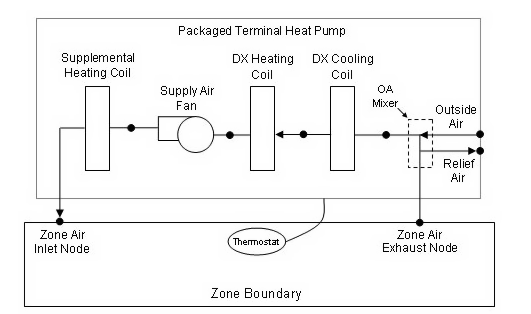
\includegraphics[width=0.9\textwidth, height=0.9\textheight, keepaspectratio=true]{media/image285.png}
\caption{Schematic of a packaged terminal heat pump (draw through fan placement) \protect \label{fig:schematic-of-a-packaged-terminal-heat-pump-001}}
\end{figure}

Links to the PTHP's supply air fan, DX coils, supplemental heating coil, and outdoor air mixer specifications are provided in the heat pump's input syntax. Additional inputs include supply and outdoor air flow rates during cooling operation, heating operation, and when neither cooling or heating is required. A description of each input field for the packaged terminal heat pump compound object is provided below.

\subsubsection{Inputs}\label{inputs-9-026}

\paragraph{Field: Name}\label{field-name-9-022}

This alpha field defines a unique user-assigned name for an instance of a packaged terminal heat pump. Any reference to this heat pump by another object will use this name.

\paragraph{Field: Availability Schedule Name}\label{field-availability-schedule-name-8-005}

This alpha field defines the name of the schedule (ref: Schedule) that denotes whether the heat pump operates during a given time period. A schedule value equal to 0 denotes that the heat pump must be off for that time period. A value greater than 0 denotes that the heat pump is available to operate during that time period. This schedule may be used to completely disable the heat pump (all of its coils and the supply air fan) as required. If this field is blank, the schedule has values of 1 for all time periods.

\paragraph{Field: Air Inlet Node Name}\label{field-air-inlet-node-name-6-000}

This alpha field defines the name of the HVAC system node from which the heat pump draws its inlet air. This node name must be the name of a zone air exhaust node (Ref. \hyperref[zonehvacequipmentconnections]{ZoneHVAC:EquipmentConnections}).

\paragraph{Field: Air Outlet Node Name}\label{field-air-outlet-node-name-6-001}

This alpha field defines the name of the HVAC system node to which the heat pump sends its outlet air. This node name must be the name of a zone air inlet node (Ref. \hyperref[zonehvacequipmentconnections]{ZoneHVAC:EquipmentConnections}).

\paragraph{Field: Outdoor Air Mixer Object Type}\label{field-outdoor-air-mixer-object-type-3}

This field specifies the type of outdoor air mixer used by this PTHP. The outdoor air mixer component is part of the PTHP compound object. The only available outdoor air mixer type is:

\begin{itemize}
\tightlist
\item
  \hyperref[outdoorairmixer]{OutdoorAir:Mixer}
\end{itemize}

This input field should be left blank when the PTHP is connected to an \textit{\hyperref[airterminalsingleductmixer]{AirTerminal:SingleDuct:Mixer}} object. If this field is left blank, an outdoor air mixer object is not simulated.

\paragraph{Field: Outdoor Air Mixer Name}\label{field-outdoor-air-mixer-name-3}

This alpha field defines the name of an outdoor air mixer component which composes part of the PTHP. Note that the return air node of the outdoor air mixer should also be the same node as the air inlet node of the PTHP. Furthermore, the outdoor air mixer's mixed air node should be the same as the PTHP's fan inlet air node (for blow through fan placement) or the PTHP's DX cooling coil inlet node (for draw through fan placement). This field should be left blank when the PTHP is connected to an \textit{\hyperref[airterminalsingleductmixer]{AirTerminal:SingleDuct:Mixer}} object.

\paragraph{Field: Cooling Supply Air Flow Rate}\label{field-cooling-supply-air-flow-rate-1-001}

This numeric field defines the supply air flow rate leaving the heat pump in cubic meters per second when the DX cooling coil is operating. Values must be greater than 0 or this field is autosizable.

\paragraph{Field: Heating Supply Air Flow Rate}\label{field-heating-supply-air-flow-rate-1-001}

This numeric field defines the supply air flow rate leaving the heat pump in cubic meters per second when the DX heating coil and/or supplemental heater are operating. Values must be greater than 0 or this field is autosizable.

\paragraph{Field: No Load Supply Air Flow Rate}\label{field-no-load-supply-air-flow-rate-1-001}

This numeric field defines the supply air flow rate leaving the heat pump in cubic meters per second when neither cooling or heating is required (i.e., DX coils and supplemental heater are off but the supply air fan operates). This field is only used when the heat pump's supply air fan operating mode schedule specifies continuous fan operation. Values must be greater than or equal to zero, or this field is autosizable. If the heat pump's supply air fan operating mode schedule specifies continuous fan operation and this value is set to zero or this field is left blank, then the model assumes that the supply air flow rate when no cooling/heating is needed is equal to the supply air flow rate when the cooling or heating coil was last operating (for cooling operation or heating operation).

\paragraph{Field: Cooling Outdoor Air Flow Rate}\label{field-cooling-outdoor-air-flow-rate-1}

This numeric field defines the outdoor air flow rate through the heat pump in cubic meters per second when the DX cooling coil is operating. Values must be greater than or equal to 0, or this field is autosizable. Note that the Cooling Outdoor Air Flow Rate is fixed; it cannot change during the simulation. In addition, the Cooling Outdoor Air Flow Rate cannot be greater than the heat pump's supply air volumetric flow rate during cooling operation.
This field is set to zero flow when the PTHP is connected to an \textit{\hyperref[airterminalsingleductmixer]{AirTerminal:SingleDuct:Mixer}} object.

\paragraph{Field: Heating Outdoor Air Flow Rate}\label{field-heating-outdoor-air-flow-rate-1}

This numeric field defines the outdoor air flow rate through the heat pump in cubic meters per second when the DX heating coil and/or supplemental heater are operating. Values must be greater than or equal to 0, or this field is autosizable. Note that the Heating Outdoor Air Flow Rate is fixed; it cannot change during the simulation. In addition, the Heating Outdoor Air Flow Rate cannot be greater than the heat pump's supply air volumetric flow rate during heating operation. This field is set to zero flow when the PTHP is connected to an \textit{\hyperref[airterminalsingleductmixer]{AirTerminal:SingleDuct:Mixer}} object.

\paragraph{Field: No Load Outdoor Air Flow Rate}\label{field-no-load-outdoor-air-flow-rate-1}

This numeric field defines the outdoor air flow rate through the heat pump in cubic meters per second when neither cooling or heating is required (i.e., DX coils and supplemental heater are off but the supply air fan operates). Values must be greater than or equal to 0, or this field is autosizable. Note that the outdoor air flow rate when no cooling/heating is needed is fixed; it cannot change during the simulation. In addition, the outdoor air flow rate when no cooling/heating is needed cannot be greater than the heat pump's supply air volumetric flow rate when no cooling/heating is needed. This field is only used when the heat pump's supply air fan operating mode schedule specifies continuous fan operation. If the heat pump's supply air fan operating mode schedule specifies continuous fan operation and the field `Supply air volumetric flow rate when no cooling or heating is needed' is set to zero or is left blank, then the model assumes that the outdoor air flow rate when no cooling/heating is needed is equal to the outdoor air flow rate when the cooling or heating coil was last operating (for cooling operation {[}i.e., Cooling Outdoor Air Flow Rate{]} or heating operation {[}i.e., Heating Outdoor Air Flow Rate{]}) and this field is not used. This field is set to zero flow when the heat pump is connected to an \textit{\hyperref[airterminalsingleductmixer]{AirTerminal:SingleDuct:Mixer}} object.

\paragraph{Field: Supply Air Fan Object Type}\label{field-supply-air-fan-object-type-6}

This alpha field defines the type of fan used by this PTHP. The only valid choices are \hyperref[fanonoff]{Fan:OnOff} and \hyperref[fanconstantvolume]{Fan:ConstantVolume}. A fan of type \hyperref[fanonoff]{Fan:OnOff} may be used with either cycling or continuous fan operating mode, and a fan of type \hyperref[fanconstantvolume]{Fan:ConstantVolume} is used only with continuous fan operating mode (see Supply Air Fan Operating Mode Schedule field below). The input requirements for these fan objects are described elsewhere in this document.

\paragraph{Field: Supply Air Fan Name}\label{field-supply-air-fan-name-5}

The name of a constant volume fan component that composes part of the PTHP. Note that the fan's maximum flow rate should be greater than or equal to the maximum supply air flow rate for the PTHP. The fan's inlet node should be the same as the outdoor air mixer's mixed air node (for blow through fan placement) or the DX heating coil's outlet node (for draw through fan placement). The fan's outlet node should be the same as the DX cooling coil's air inlet node (for blow through fan placement) or the supplemental heater's air inlet node (for draw through fan placement).

\paragraph{Field: Heating Coil Object Type}\label{field-heating-coil-object-type-4-000}

This alpha field defines the type of DX heating coil to be used by this PTHP. The only valid choice are \textbf{\hyperref[coilheatingdxsinglespeed]{Coil:Heating:DX:SingleSpeed}} and \textbf{\hyperref[coilheatingdxvariablespeed]{Coil:Heating:DX:VariableSpeed}}. The input requirements for this DX heating coil object are described elsewhere in this document.

\paragraph{Field: Heating Coil Name}\label{field-heating-coil-name-4-000}

This alpha field defines the name of the DX heating coil used by this PTHP, and this name should match the name specified in the corresponding DX heating coil object.

\paragraph{Field: Heating Convergence Tolerance}\label{field-heating-convergence-tolerance-3}

This numeric field defines the convergence tolerance for the unit's heating output. This field allows the user some control over how closely the heat pump will control the air-side conditions. The relative size of this parameter relates directly to the closeness of the control. A very small value in this field will result in tight control and will probably result in larger numbers of iterations. A large value in this field will result in looser controls and could result in unsatisfactory fluctuations in zone air temperature. Initial experience with this parameter lends to the recommendation of using 0.001 as the starting point.

The heat pump is controlled by matching its sensible (temperature) heating output to the zone sensible load (demand). Because the performance of the DX heating coil is frequently non-linear, the heat pump model must call the DX heating coil model several times (iterate) to determine the proper run time fraction to meet the zone load. The heating convergence tolerance is the error tolerance used to terminate the iteration procedure when the following equation is satisfied:

\begin{equation}
\frac{{\left| {({Q_{ZoneLoad}} - {Q_{HeatPump,out}})} \right|}}{{{Q_{ZoneLoad}}}}\,\, \le \,\,Heating{\kern 1pt} Convergence{\kern 1pt} Tolerance
\end{equation}

The maximum number of iterations is limited, with a warning message generated if the above equation is not satisfied within the maximum number of iterations.

\paragraph{Field: Cooling Coil Object Type}\label{field-cooling-coil-object-type-4-000}

This alpha field defines the type of DX cooling coil used by this PTHP. The input requirements for these DX cooling coil objects are described elsewhere in this document. Only allowable coil types are:

\begin{itemize}
\item
  \hyperref[coilcoolingdxsinglespeed]{Coil:Cooling:DX:SingleSpeed}
\item
  \hyperref[coilsystemcoolingdxheatexchangerassisted]{CoilSystem:Cooling:DX:HeatExchangerAssisted}
\item
  \hyperref[coilcoolingdxvariablespeed]{Coil:Cooling:DX:VariableSpeed}
\end{itemize}

\paragraph{Field: Cooling Coil Name}\label{field-cooling-coil-name-3-000}

This alpha field defines the name of the cooling coil used by this PTHP, and this name should match the name specified in the corresponding DX cooling coil object.

\paragraph{Field: Cooling Convergence Tolerance}\label{field-cooling-convergence-tolerance-3}

This numeric field defines the convergence tolerance for the unit's cooling output. This field allows the user some control over how closely the heat pump will control the air-side conditions. The relative size of this parameter relates directly to the closeness of the control. A very small value in this field will result in tight control and will probably result in larger numbers of iterations. A large value in this field will result in looser controls and could result in unsatisfactory fluctuations in zone air temperature. Initial experience with this parameter lends to the recommendation of using 0.001 as the starting point.

The heat pump is controlled by matching its sensible (temperature) cooling output to the zone sensible load (demand). Because the performance of the DX cooling coil is frequently non-linear, the heat pump model must call the DX cooling coil model several times (iterate) to determine the proper run time fraction to meet the zone load. The cooling convergence tolerance is the error tolerance used to terminate the iteration procedure when the following equation is satisfied:

\begin{equation}
\frac{{\left| {({Q_{ZoneLoad}} - {Q_{HeatPump,out}})} \right|}}{{{Q_{ZoneLoad}}}}\,\, \le \,\,Cooling{\kern 1pt} Convergence{\kern 1pt} Tolerance
\end{equation}

The maximum number of iterations is limited, with a warning message generated if the above equation is not satisfied within the maximum number of iterations.

\paragraph{Field: Supplemental Heating Coil Object Type}\label{field-supplemental-heating-coil-object-type-000}

This alpha field defines the type of supplemental heating coil to be used by this PTHP. The input requirements for these heating coil objects are described elsewhere in this document. The hot water and steam heating coils require specifying plant loop, branches, and connector objects to support the heating coils, and are placed on the demand side of the plantloop. The hot water flow modulation through the supplemental heating coil does not require additional controller or \hyperref[controllerwatercoil]{Controller:WaterCoil} object. The parent object (PTHP) itself provides the ``controller'' function of modulating water flow. Allowable coil types are:

\begin{itemize}
\item
  \hyperref[coilheatingelectric]{Coil:Heating:Electric}
\item
  \hyperref[coilheatinggas-000]{Coil:Heating:Fuel}
\item
  \hyperref[coilheatingwater]{Coil:Heating:Water}
\item
  \hyperref[coilheatingsteam]{Coil:Heating:Steam}
\end{itemize}

\paragraph{Field: Supplemental Heating Coil Name}\label{field-supplemental-heating-coil-name-000}

This alpha field defines the name of the supplemental heating coil used by this PTHP, and this name should match the name specified in the corresponding heating coil object.

\paragraph{Field: Maximum Supply Air Temperature from Supplemental Heater}\label{field-maximum-supply-air-temperature-from-supplemental-heater-000}

This numeric field defines the maximum supply air temperature in degrees Celsius exiting the heat pump supplemental heater coil. The supplemental heater will be controlled so that its supply air temperature does not exceed this value. This field is autosizable.

\paragraph{Field: Maximum Outdoor Dry-Bulb Temperature for Supplemental Heater Operation}\label{field-maximum-outdoor-dry-bulb-temperature-for-supplemental-heater-operation-000}

This numeric field defines the maximum outdoor dry-bulb temperature in degrees Celsius for PTHP supplemental heater operation. The supplemental heater will not operate when the outdoor dry-bulb temperature is above this value. The maximum value must be less than or equal to 21\si{\degreeCelsius}. If this field is left blank, the default value is 21\si{\degreeCelsius}.

\paragraph{Field: Fan Placement}\label{field-fan-placement-4-000}

This alpha field has two choices: \textbf{BlowThough} or \textbf{DrawThrough}. The first choice stands for ``blow through fan''. This means that the unit consists of an outdoor air mixer followed by a fan followed by the DX coils and supplemental heating coil. The fan ``blows through'' the cooling and heating coils. The second choice stands for ``draw through fan''. This means that the unit consists of an outdoor air mixer followed by the DX coil(s) followed by a fan, with the supplemental heater located at the outlet of the fan. The fan ``draws air through'' the DX coil(s). If this field is left blank, the default is draw through.

Note: the packaged terminal heat pump's supply air fan, cooling coil, heating coil and supplementary heating coil must be connected according to the configuration shown above (Figure~\ref{fig:schematic-of-a-packaged-terminal-heat-pump-001}) for the draw through fan configuration. The only other valid configuration is with a blow through fan placement, where the fan is located between the outdoor air mixer and the DX cooling coil.

\paragraph{Field: Supply Air Fan Operating Mode Schedule Name}\label{field-supply-air-fan-operating-mode-schedule-name-5}

This alpha field specifies the name of the supply air fan operating mode schedule. The supply air fan operating mode may vary during the simulation based on time-of-day or with a change of season. Schedule values of 0 denote that the supply air fan and the heating or cooling coil cycle on and off together to meet the heating or cooling load (a.k.a. AUTO fan). Schedule values other than 0 denote that the supply air fan runs continuously while the heating or cooling coil cycles to meet the load. If this field is left blank, the model assumes the supply air fan cycles with the heating or cooling coil throughout the simulation.

\paragraph{Field: Availability Manager List Name}\label{field-availability-manager-list-name-7}

This optional input field is the name of an \hyperref[availabilitymanagerassignmentlist]{AvailabilityManagerAssignmentList} object. An Availability Manager Assignment List is a list of Availability Managers giving both Availability Manager type and name. The availability managers in the list apply to this packaged terminal heat pump or object's fan. If the packaged terminal heat pump is available (per the Availability Schedule Name input field above) and this input field has a valid availability manager assignment list name, then the availability managers in the list determine when and if the fan of this packaged terminal heat pump object should be on or off.

\paragraph{Field: Design Specification ZoneHVAC Sizing Object Name}\label{field-design-specification-zonehvac-sizing-object-name-7}

This optional input field is the name of a \hyperref[designspecificationzonehvacsizing]{DesignSpecification:ZoneHVAC:Sizing} object. The name must correspond to unique name of a \hyperref[designspecificationzonehvacsizing]{DesignSpecification:ZoneHVAC:Sizing} object. A Design Sepcification Zone HVAC Sizing object defines scalable sizing methods for sizing input fields such as Cooling Supply Air Flow Rate in this PTHP zone HVAC object. The scaled Supply Air Flow Rate in turn is used to size cooling and heating capacity of the unit.

\paragraph{Field: Capacity Control Method}\label{field-capacity-control-method-3}

This input denotes how the unit's output is controlled in order to meet zone heating or cooling requirement. The choices are \textbf{\emph{None}} or \textbf{\emph{SingleZoneVAV}}. For \emph{None}, the unit varies the fan and/or coil speed to meet the load. If constant fan operating mode is selected the fan operates at the design cooling or heating air flow rate while the coil modulates to meet the load. If cycling fan operating mode is selected the fan and coil modulate in unison to meet the load. For \emph{SingleZoneVAV}, the fan air flow rate is reduced to the no load supply air flow rate when the zone sensible load is low such that the maximum supply air temperature limit is not exceeded. If the unit cannot meet the load at this lower air flow rate, the fan speed increases while maintaining the maximum supply air temperature. If the unit still cannot meet the load the unit will operate at the maximum supply air flow rate and the maximum supply air temperature limit can be exceeded. Supply air temperature limits are identified in the input fields for Minimum Supply Air Temperature in Cooling Mode and Maximum Supply Air Temperature in Heating Mode. Additionally, specific coil types are required for the SingleZoneVAV capacity control method. The cooling coil type is \hyperref[coilcoolingdxsinglespeed]{Coil:Cooling:DX:SingleSpeed} while the heating coil type is \hyperref[coilheatingdxsinglespeed]{Coil:Heating:DX:SingleSpeed}.

\paragraph{Field: Minimum Supply Air Temperature in Cooling Mode}\label{field-minimum-supply-air-temperature-in-cooling-mode-3}

When Capacity Control Method = SingleZoneVAV, enter the minimum air temperature limit for reduced fan speed in cooling mode. For SingleZoneVAV, this field's minimum supply air temperature is 0.0\si{\degreeCelsius}. This field is autosizable and the default is autosize.

\paragraph{Field: Maximum Supply Air Temperature in Heating Mode}\label{field-maximum-supply-air-temperature-in-heating-mode-3}

When Capacity Control Method = SingleZoneVAV, enter the maximum air temperature limit for reduced fan speed in heating mode. For SingleZoneVAV, this field's minimum supply air temperature is 0.0\si{\degreeCelsius}. This field is autosizable and the default is autosize.


As shown in the example below, correct specification of the packaged terminal heat pump requires the following objects in addition to the compound object itself:

\begin{enumerate}
\def\labelenumi{\arabic{enumi})}
\item
  Fan (\hyperref[fanonoff]{Fan:OnOff} or \hyperref[fanconstantvolume]{Fan:ConstantVolume})
\item
  DX cooling coil (\hyperref[coilcoolingdxsinglespeed]{Coil:Cooling:DX:SingleSpeed} or \hyperref[coilsystemcoolingdxheatexchangerassisted]{CoilSystem:Cooling:DX:HeatExchangerAssisted})
\item
  DX heating coil (\hyperref[coilheatingdxsinglespeed]{Coil:Heating:DX:SingleSpeed})
\item
  Supplemental heating coil (\hyperref[coilheatinggas-000]{Coil:Heating:Fuel} or \hyperref[coilheatingelectric]{Coil:Heating:Electric})
\item
  \hyperref[outdoorairmixer]{OutdoorAir:Mixer}
\end{enumerate}

\begin{lstlisting}

ZoneHVAC:PackagedTerminalHeatPump,
  Zone2PTHP,               !- Name
  FanAndCoilAvailSched,    !- Availability Schedule Name
  Zone2PTHPAirInletNode,   !- Air Inlet Node Name
  Zone2PTHPAirOutletNode,  !- Air Outlet Node Name
  OutdoorAir:Mixer,        !- Outdoor Air Mixer Object Type
  Zone2PTHPOAMixer,        !- Outdoor Air Mixer Name
  autosize,                !- Cooling Supply Air Flow Rate {m3/s}
  autosize,                !- Heating Supply Air Flow Rate {m3/s}
  autosize,                !- No Load Supply Air Flow Rate {m3/s}
  autosize,                !- Cooling Outdoor Air Flow Rate {m3/s}
  autosize,                !- Heating Outdoor Air Flow Rate {m3/s}
  autosize,                !- No Load Outdoor Air Flow Rate {m3/s}
  Fan:OnOff,               !- Supply Air Fan Object Type
  Zone2PTHPFan,            !- Supply Air Fan Name
  Coil:Heating:DX:SingleSpeed,  !- Heating Coil Object Type
  Zone2PTHPDXHeatCoil,     !- Heating Coil Name
  0.001,                   !- Heating Convergence Tolerance {dimensionless}
  Coil:Cooling:DX:SingleSpeed,  !- Cooling Coil Object Type
  Zone2PTHPDXCoolCoil,     !- Cooling Coil Name
  0.001,                   !- Cooling Convergence Tolerance {dimensionless}
  Coil:Heating:Electric,   !- Supplemental Heating Coil Object Type
  Zone2PTHPSupHeater,      !- Supplemental Heating Coil Name
  autosize,                !- Maximum Supply Air Temperature from Supplemental Heater {C}
  10.0,                    !- Maximum Outdoor Dry-Bulb Temperature for Supplemental Heater Operation {C}
  BlowThrough,             !- Fan Placement
  CyclingFanSch;           !- Supply Air Fan Operating Mode Schedule Name


  Schedule:Compact,
      CyclingFanSch,               !- Name
      Fraction,                    !- ScheduleType
      Through: 12/31,              !- Complex Field \#1
      For: AllDays,                !- Complex Field \#2
      Until: 24:00,                !- Complex Field \#7
      0.0;                         !- Complex Field \#8

  OutdoorAir:Mixer,
      Zone2PTHPOAMixer,            !- Name
      Zone2PTHPOAMixerOutletNode,  !-Mixed Air Node Name
      Zone2PTHPOAInNode,           !-Outdoor Air Stream Node Name
      Zone2PTHPExhNode,            !- Relief Air Stream Node Name
      Zone2PTHPAirInletNode;       !- Return Air Stream Node Name

  Fan:OnOff,
      Zone2PTHPFan,                !- Name
      FanAndCoilAvailSched,        !- Availability Schedule Name
      0.5,                         !- Fan Total Efficiency
      75.0,                        !- Pressure Rise {Pa}
      autosize,                    !- Maximum Flow Rate {m3/s}
      0.9,                         !- Motor Efficiency
      1.0,                         !- Motor In Airstream Fraction
      Zone2PTHPOAMixerOutletNode,  !- Air Inlet Node Name
      Zone2PTHPFanOutletNode;      !- Air Outlet Node Name

  Coil:Cooling:DX:SingleSpeed,
      Zone2PTHPDXCoolCoil,         !- Coil Name
      CoolingCoilAvailSched,       !- Availability Schedule
      autosize,                    !- Rated Total Cooling Capacity (gross) {W}
      autosize,                    !- Rated SHR
      3.0,                         !- Rated COP
      autosize,                    !- Rated Air Volume Flow Rate {m3/s}
      Zone2PTHPFanOutletNode,      !- Coil Air Inlet Node
      Zone2PTHPCoolCoilOutletNode, !- Coil Air Outlet Node
      HPACCoolCapFT,               !- Total Cooling Capacity Modifier Curve (function of temperature)
      HPACCoolCapFFF,              !- Total Cooling Capacity Modifier Curve (function of flow fraction)
      HPACEIRFT,                   !- Energy Input Ratio Modifier Curve (function of temperature)
      HPACEIRFFF,                  !- Energy Input Ratio Modifier Curve (function of flow fraction)
      HPACPLFFPLR;                 !- Part Load Fraction Correlation (function of part load ratio)

  COIL:Heating:DX:SingleSpeed,
      Zone2PTHPDXHeatCoil,         !- Coil Name
      HeatingCoilAvailSched,       !- Availability Schedule
      autosize,                    !- Rated Total Heating Capacity {W}
      2.75,                        !- Rated COP
      autosize,                    !- Rated Air Volume Flow Rate {m3/s}
      Zone2PTHPCoolCoilOutletNode, !- Coil Air Inlet Node
      Zone2PTHPDXHeatCoilOutletNode, !- Coil Air Outlet Node
      HPACHeatCapFT,              !- Total heating capacity modifier curve (function of temperature)
      HPACHeatCapFFF,             !- Total heating capacity modifier curve (function of flow fraction)
      HPACHeatEIRFT,              !- Energy input ratio modifier curve (function of temperature)
      HPACHeatEIRFFF,             !- Energy input ratio modifier curve (function of flow fraction)
      HPACCOOLPLFFPLR,            !- Part load fraction correlation (function of part load ratio)
      ,                           !- Defrost energy input ratio modifier curve (function of temperature)
      2.0,                        !- Minimum Outdoor Dry-bulb Temperature for Compressor Operation {C}
      5.0,                        !- Maximum Outdoor Dry-bulb Temperature for Defrost Operation {C}
      200.0,                      !- Crankcase Heater Capacity {W}
      10.0,                       !- Maximum Outdoor Dry-bulb Temperature for Crankcase Heater Operation {C}
      Resistive,                  !- Defrost Strategy
      TIMED,                      !- Defrost Control
      0.166667,                   !- Defrost Time Period Fraction
      20000;                      !- Resistive Defrost Heater Capacity {W}

  Coil:Heating:Electric,
      Zone2PTHPSupHeater,          !- Name
      HeatingCoilAvailSched,       !- Availability Schedule Name
      1.0,                         !- Efficiency
      autosize,                    !- Nominal Capacity {W}
      Zone2PTHPDXHeatCoilOutletNode, !- Air Inlet Node Name
      Zone2PTHPAirOutletNode;      !- Air Outlet Node Name
\end{lstlisting}

\subsubsection{Outputs}\label{outputs-8-009}

\begin{itemize}
\item
  HVAC,Average,Zone Packaged Terminal Heat Pump Total Heating Rate {[}W{]}
\item
  HVAC,Sum,Zone Packaged Terminal Heat Pump Total Heating Energy {[}J{]}
\item
  HVAC,Average,Zone Packaged Terminal Heat Pump Total Cooling Rate {[}W{]}
\item
  HVAC,Sum,Zone Packaged Terminal Heat Pump Total Cooling Energy {[}J{]}
\item
  HVAC,Average,Zone Packaged Terminal Heat Pump Sensible Heating Rate {[}W{]}
\item
  HVAC,Sum,Zone Packaged Terminal Heat Pump Sensible Heating Energy {[}J{]}
\item
  HVAC,Average,Zone Packaged Terminal Heat Pump Sensible Cooling Rate {[}W{]}
\item
  HVAC,Sum,Zone Packaged Terminal Heat Pump Sensible Cooling Energy {[}J{]}
\item
  HVAC,Average,Zone Packaged Terminal Heat Pump Latent Heating Rate {[}W{]}
\item
  HVAC,Sum,Zone Packaged Terminal Heat Pump Latent Heating Energy {[}J{]}
\item
  HVAC,Average,Zone Packaged Terminal Heat Pump Latent Cooling Rate {[}W{]}
\item
  HVAC,Sum,Zone Packaged Terminal Heat Pump Latent Cooling Energy {[}J{]}
\item
  HVAC,Average,Zone Packaged Terminal Heat Pump Electricity Rate {[}W{]}
\item
  HVAC,Sum,Zone Packaged Terminal Heat Pump Electricity Energy {[}J{]}
\item
  HVAC,Average,Zone Packaged Terminal Heat Pump Fan Part Load Ratio {[]}
\item
  HVAC,Average,Zone Packaged Terminal Heat Pump Compressor Part Load Ratio {[]}
\item
  HVAC,Average,Zone Packaged Terminal Heat Pump Fan Availability Status {[]}
\end{itemize}

\paragraph{Zone Packaged Terminal Heat Pump Total Heating Rate {[}W{]}}\label{zone-packaged-terminal-heat-pump-total-heating-rate-w}

This output field is the total (enthalpy) heat addition rate of the packaged terminal heat pump to the zone it is serving in Watts. This value is calculated using the enthalpy difference of the heat pump outlet air and inlet air streams, and the air mass flow rate through the heat pump. This value is calculated for each HVAC system timestep being simulated, and the results (enthalpy addition only) are averaged for the timestep being reported.

\paragraph{Zone Packaged Terminal Heat Pump Total Heating Energy {[}J{]}}\label{zone-packaged-terminal-heat-pump-total-heating-energy-j}

This output field is the total (enthalpy) heat addition of the packaged terminal heat pump to the zone it is serving in Joules over the timestep being reported. This value is calculated using the enthalpy difference of the heat pump outlet air and inlet air streams, the air mass flow rate through the heat pump, and the HVAC simulation timestep. This value is calculated for each HVAC system timestep being simulated, and the results (enthalpy addition only) are summed for the timestep being reported.

\paragraph{Zone Packaged Terminal Heat Pump Total Cooling Rate {[}W{]}}\label{zone-packaged-terminal-heat-pump-total-cooling-rate-w}

This output field is the total (enthalpy) heat extraction rate of the packaged terminal heat pump from the zone it is serving in Watts. This value is calculated using the enthalpy difference of the heat pump outlet air and inlet air streams, and the air mass flow rate through the heat pump. This value is calculated for each HVAC system timestep being simulated, and the results (enthalpy extraction only) are averaged for the timestep being reported.

\paragraph{Zone Packaged Terminal Heat Pump Total Cooling Energy {[}J{]}}\label{zone-packaged-terminal-heat-pump-total-cooling-energy-j}

This output field is the total (enthalpy) heat extraction of the packaged terminal heat pump from the zone it is serving in Joules over the timestep being reported. This value is calculated using the enthalpy difference of the heat pump outlet air and inlet air streams, the air mass flow rate through the heat pump, and the HVAC simulation timestep. This value is calculated for each HVAC system timestep being simulated, and the results (enthalpy extraction only) are summed for the timestep being reported.

\paragraph{Zone Packaged Terminal Heat Pump Sensible Heating Rate {[}W{]}}\label{zone-packaged-terminal-heat-pump-sensible-heating-rate-w}

This output field is the sensible heat addition rate of the packaged terminal heat pump to the zone it is serving in Watts. This value is calculated using the enthalpy difference of the heat pump outlet air and inlet air streams at a constant humidity ratio, and the air mass flow rate through the heat pump. This value is calculated for each HVAC system timestep being simulated, and the results (heating only) are averaged for the timestep being reported.

\paragraph{Zone Packaged Terminal Heat Pump Sensible Heating Energy {[}J{]}}\label{zone-packaged-terminal-heat-pump-sensible-heating-energy-j}

This output field is the sensible heat addition of the packaged terminal heat pump to the zone it is serving in Joules over the timestep being reported. This value is calculated using the enthalpy difference of the heat pump outlet air and inlet air streams at a constant humidity ratio, the air mass flow rate through the heat pump, and the HVAC simulation timestep. This value is calculated for each HVAC system timestep being simulated, and the results (heating only) are summed for the timestep being reported.

\paragraph{Zone Packaged Terminal Heat Pump Sensible Cooling Rate {[}W{]}}\label{zone-packaged-terminal-heat-pump-sensible-cooling-rate-w}

This output field reports the moist air sensible heat extraction rate of the packaged terminal heat pump from the zone it is serving in Watts. This value is calculated using the enthalpy difference of the heat pump outlet air and inlet air streams at a constant humidity ratio, and the air mass flow rate through the heat pump. This value is calculated for each HVAC system timestep being simulated, and the results (cooling only) are averaged for the timestep being reported.

\paragraph{Zone Packaged Terminal Heat Pump Sensible Cooling Energy {[}J{]}}\label{zone-packaged-terminal-heat-pump-sensible-cooling-energy-j}

This output field reports the moist air sensible heat extraction of the packaged terminal heat pump from the zone it is serving in Joules over the timestep being reported. This value is calculated using the enthalpy difference of the heat pump outlet air and inlet air streams at a constant humidity ratio, the air mass flow rate through the heat pump, and the HVAC simulation timestep. This value is calculated for each HVAC system timestep being simulated, and the results (cooling only) are summed for the timestep being reported.

\paragraph{Zone Packaged Terminal Heat Pump Latent Heating Rate {[}W{]}}\label{zone-packaged-terminal-heat-pump-latent-heating-rate-w}

This output field is the latent heat addition (humidification) rate of the packaged terminal heat pump to the zone it is serving in Watts. This value is calculated as the difference between the total energy rate and the sensible energy rate provided by the packaged terminal heat pump. This value is calculated for each HVAC system timestep being simulated, and the results (latent heat addition only) are averaged for the timestep being reported.

\paragraph{Zone Packaged Terminal Heat Pump Latent Heating Energy {[}J{]}}\label{zone-packaged-terminal-heat-pump-latent-heating-energy-j}

This output field is the latent heat addition (humidification) of the packaged terminal heat pump to the zone it is serving in Joules over the timestep being reported. This value is calculated as the difference between the total energy delivered to the zone and the sensible energy delivered to the zone by the packaged terminal heat pump. This value is calculated for each HVAC system timestep being simulated, and the results (latent heat addition only) are summed for the timestep being reported.

\paragraph{Zone Packaged Terminal Heat Pump Latent Cooling Rate {[}W{]}}\label{zone-packaged-terminal-heat-pump-latent-cooling-rate-w}

This output field is the latent heat extraction (dehumidification) rate of the packaged terminal heat pump from the zone it is serving in Watts. This value is calculated as the difference between the total energy rate and the sensible energy rate provided by the packaged terminal heat pump. This value is calculated for each HVAC system timestep being simulated, and the results (latent heat extraction only) are averaged for the timestep being reported.

\paragraph{Zone Packaged Terminal Heat Pump Latent Cooling Energy {[}J{]}}\label{zone-packaged-terminal-heat-pump-latent-cooling-energy-j}

This output field is the latent heat extraction (dehumidification) of the packaged terminal heat pump from the zone it is serving in Joules over the timestep being reported. This value is calculated as the difference between the total energy delivered to the zone and the sensible energy delivered to the zone by the packaged terminal heat pump. This value is calculated for each HVAC system timestep being simulated, and the results (latent heat extraction only) are summed for the timestep being reported.

\paragraph{Zone Packaged Terminal Heat Pump Electricity Rate {[}W{]}}\label{zone-packaged-terminal-heat-pump-electric-power-w}

This output field is the electricity consumption rate of the packaged terminal heat pump in Watts. The consumption includes electricity used by the compressor (including crankcase heater), fans (indoor supply air fan and the condenser fan), and the supplemental heating coil (if electric). This value is calculated for each HVAC system timestep being simulated, and the results are averaged for the timestep being reported.

\paragraph{Zone Packaged Terminal Heat Pump Electricity Energy {[}J{]}}\label{zone-packaged-terminal-heat-pump-electric-energy-j}

This output field is the electricity consumption of the packaged terminal heat pump in Joules for the time period being reported. The consumption includes electricity used by the compressor (including crankcase heater), fans (indoor supply air fan and the condenser fan), and the supplemental heating coil (if electric). This value is calculated for each HVAC system timestep being simulated, and the results are summed for the timestep being reported.

\paragraph{Zone Packaged Terminal Heat Pump Fan Part Load Ratio {[]}}\label{zone-packaged-terminal-heat-pump-fan-part-load-ratio}

This output field is the part-load ratio of the fan. The fan part-load ratio is defined as the average supply air mass flow rate divided by the maximum supply air mass flow rate. The maximum supply air mass flow rate depends on whether heating, cooling, or no heating or cooling is required during the timestep. This value is calculated for each HVAC system timestep being simulated, and the results are averaged for the timestep being reported.

\paragraph{Zone Packaged Terminal Heat Pump Compressor Part Load Ratio {[]}}\label{zone-packaged-terminal-heat-pump-compressor-part-load-ratio}

This output field is the part-load ratio of the compressor used by the DX coils (cooling and heating). Compressor part-load ratio is defined as the total coil load divided by the coil steady-state capacity. This value is calculated for each HVAC system timestep being simulated, and the results are averaged for the timestep being reported.

\paragraph{Zone Packaged Terminal Heat Pump Fan Availability Status {[]}}\label{zone-packaged-terminal-heat-pump-fan-availability-status}

This is the availability status of the packaged terminal heat pump~ fan. This status flag is a result of the calculations made by the Availability Manager(s) listed in an AvailabilityManagerAssignmentList object and/or calculations made by Hybrid Ventilation Manager object. The AvailabilityManagerAssignmentList is an optional input in the packaged terminal heat pump~ object. When a single availability manager is used in an Availability Manager Assignment List, this is also the availability status reported by the specific availability manager (Ref. AvailabilityManager:* Outputs). For multiple availability managers in an Availability Manager Assignment List (with or without Hybrid Ventilation Manager), rules to determine fan availability status are described in the section `Group -- System Availability Managers'. The control status outputs are represented using integers 0 through 3. These integers represent NoAction (0), ForceOff (1), CycleOn (2), and CycleOnZoneFansOnly (3). Since the status output is averaged, the output result may not correspond to the values described here when output variable frequencies other than detailed are used. Use the ``detailed'' reporting frequency (Ref. Output:Variable object) to view the availability status at each simulation timestep.

\subsection{ZoneHVAC:RefrigerationChillerSet}\label{zonehvacrefrigerationchillerset}

The ZoneHVAC:RefrigerationChillerSet object works in conjunction with one or multiple air chillers, compressor racks, refrigeration systems, or refrigeration secondary system objects (Ref. \hyperref[refrigerationairchiller]{Refrigeration:AirChiller} \hyperref[refrigerationcompressorrack]{Refrigeration:CompressorRack}, \hyperref[refrigerationsystem]{Refrigeration:System}, or \hyperref[refrigerationsecondarysystem]{Refrigeration:SecondarySystem}) to simulate the performance of a group of air chillers cooling a single zone. The chiller set model passes information about the zone conditions to determine the performance of individual chiller coils within the set, thus providing the sensible and latent heat exchange with the zone environment.

The refrigeration chiller set object inputs include a name, an availability schedule name, the name of the zone cooled by the chiller set, the air inlet node name, the air outlet node name, and an extensible list of air chiller names (Ref. \hyperref[refrigerationairchiller]{Refrigeration:AirChiller}).

\subsubsection{Inputs}\label{inputs-10-024}

\paragraph{Field: Name}\label{field-name-10-020}

A unique user-assigned name for an instance of a refrigeration chiller. Any reference to this refrigeration chiller by another object (may be listed in a \hyperref[refrigerationcaseandwalkinlist]{Refrigeration:CaseAndWalkInList}, \hyperref[refrigerationsystem]{Refrigeration:System}, \hyperref[refrigerationsecondarysystem]{Refrigeration:SecondarySystem}, or \hyperref[refrigerationcompressorrack]{Refrigeration:CompressorRack}) will use this name.

\paragraph{Field: Availability Schedule Name}\label{field-availability-schedule-name-9-002}

The name of the schedule (ref: Schedule) that denotes whether the refrigeration chiller can operate during a given time period. A schedule value greater than 0 (maximum schedule value of 1.0 is typically used) indicates that the refrigeration chiller will operate during a given time period. A value equal to 0 denotes that the case does not operate (everything is OFF: refrigeration, fans, lights, anti-sweat, etc.). Typically the refrigeration chiller will operate throughout the day (i.e., the schedule will contain 1 for all time periods); however, refrigeration chillers require maintenance and/or cleaning and this can be modeled accordingly using this schedule if desired. If this field is left blank, the default schedule has a value of 1 for all time periods.

\paragraph{Field: Zone Name}\label{field-zone-name-1-011}

A unique user-assigned name for the zone cooled by this refrigeration chiller. This zone must represent a conditioned space, that is, it must appear in a \hyperref[zonehvacequipmentconnections]{ZoneHVAC:EquipmentConnections} object.

\paragraph{Field: Air Inlet Node Name}\label{field-air-inlet-node-name-7-000}

Not used, reserved for future use.~ Current version exchanges energy directly with the zone, external of any air system. (Future: The name of the zone exhaust node (see Node) from which the refrigeration chiller draws its indoor air. This should be one of the zone exhaust nodes for the zone cooled by the chiller set.)

\paragraph{Field: Air Outlet Node Name}\label{field-air-outlet-node-name-7-001}

Not used, reserved for future use.~ Current version exchanges energy directly with the zone, external of any air system. (Future: The name of the node where the chiller coil sends its outlet air, which must be one of the inlet air nodes for the zone which is being cooled.)

\paragraph{Field: Air Chiller \#1 ~Name}\label{field-air-chiller-1-name}

The name of the first air chiller that will be used to meet the zone cooling load.

\paragraph{Field: Air Chiller \#2 ~Name}\label{field-air-chiller-2-name}

The name of the second air chiller that will be used to meet the zone cooling load.

\paragraph{Field: Air Chiller \#3 ~Name}\label{field-air-chiller-3-name}

The name of the third air chiller that will be used to meet the zone cooling load.

\paragraph{Field: Air Chiller \#n ~Name (Extensible list, 20 provided in the IDD)}\label{field-air-chiller-n-name-extensible-list-20-provided-in-the-idd}

The name of the nth air chiller that will be used to meet the zone cooling load.

The following is an example input for a refrigeration chiller set.

\begin{lstlisting}

   ZoneHVAC:RefrigerationChillerSet,
      SubFreezerChillerSet ,     !- Name
      ,                         !- Availability Schedule Name
      SubFreezer,                !- Zone Name
      NODE_142,                   !- Air Inlet Node Name
      NODE_141,                   !- Air Outlet Node Name
      SubFreezerAirChiller_1,    !- Air Chiller \#1 Name
      SubFreezerAirChiller_2,    !- Air Chiller \#2 Name
      SubFreezerAirChiller_3;    !- Air Chiller \#3 Name
\end{lstlisting}

There are no outputs variables for a ZoneHVAC:RefrigerationChillerSet. Outputs for the refrigeration impact on any zone are listed in the Group:Refrigeration.

\subsection{ZoneHVAC:WaterToAirHeatPump}\label{zonehvacwatertoairheatpump}

The zone water-to-air heat pump is a compound component consisting of a fan, water-to-air cooling and heating coils, and a supplemental heating coil. Links to the fan, WaterToAirHeatPump cooling coil, WaterToAirHeatPump heating coil, and supplementary heating coil specifications are provided in the heat pump's input data syntax. The heat pump switches between cooling and heating depending on the zone's demand. The load side (air) of the zone water-to-air heat pump consists of an On/Off fan component, a WaterToAirHeatPump cooling coil component, a WaterToAirHeatPump heating coil component, and a Gas or Electric supplemental heating coil component. The source side (water) of the heat pump is connected to a condenser loop with a heat exchanger (ground heat exchanger or other type) or a plant loop with a heating source such as a boiler and a cooling source such as a chiller or cooling tower.~ The diagram below shows the setup and connection of the heat pump for the source side and load side for a ground heat exchanger configuration. Note that on the load side, the WaterToAirHeatPump cooling coil must always be placed before the WaterToAirHeatPump heating coil.

For this zone heat pump,there are two types of WaterToAirHeatPump coil model allowed:

\begin{itemize}
\item
  \hyperref[coilcoolingwatertoairheatpumpequationfit]{Coil:Cooling:WaterToAirHeatPump:EquationFit}
\item
  \hyperref[coilheatingwatertoairheatpumpequationfit]{Coil:Heating:WaterToAirHeatPump:EquationFit}
\item
  \hyperref[coilcoolingwatertoairheatpumpvariablespeedequationfit]{Coil:Cooling:WaterToAirHeat\hyperref[pumpvariablespeed]{Pump:VariableSpeed}EquationFit}
\item
  \hyperref[coilheatingwatertoairheatpumpvariablespeedequationfit]{Coil:Heating:WaterToAirHeat\hyperref[pumpvariablespeed]{Pump:VariableSpeed}EquationFit}
\end{itemize}

\begin{figure}[hbtp] % fig 113
\centering
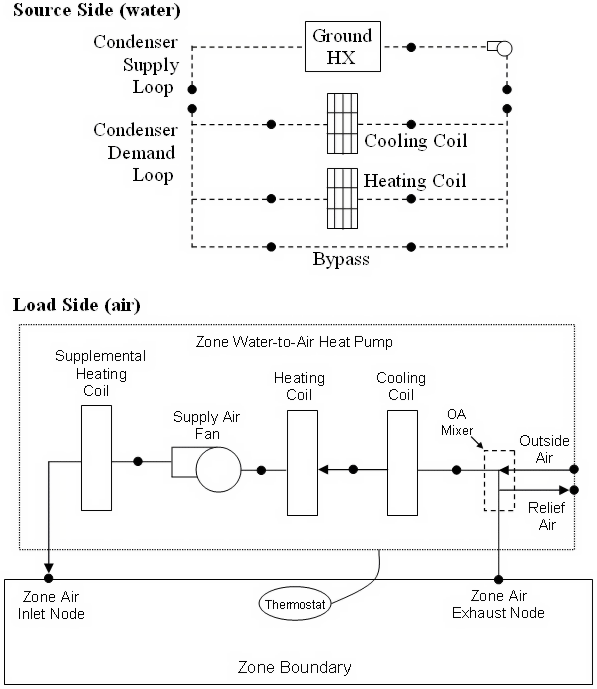
\includegraphics[width=0.9\textwidth, height=0.9\textheight, keepaspectratio=true]{media/image288.png}
\caption{Zone Water to Air Heat Pump Schematic for a DrawThrough Configuration with Ground Heat Exchanger \protect \label{fig:zone-water-to-air-heat-pump-schematic-for-a}}
\end{figure}

\subsubsection{Inputs}\label{inputs-11-023}

\paragraph{Field: Name}\label{field-name-11-017}

This alpha field contains the identifying name for the zone system heat pump.

\paragraph{Field: Availability Schedule Name}\label{field-availability-schedule-name-10-001}

This alpha field defines the name of the schedule (ref: Schedule) that denotes whether the heat pump operates during a given time period. A schedule value equal to 0 denotes that the heat pump must be off for that time period. A value greater than 0 denotes that the heat pump is available to operate during that time period. This schedule may be used to completely disable the heat pump (all of its coils and the supply air fan) as required. If this field is blank, the schedule has values of 1 for all time periods.

\paragraph{Field: Air Inlet Node Name}\label{field-air-inlet-node-name-8-000}

This alpha field contains the name of the HVAC system node from which the heat pump draws its inlet air. This node must be a zone exhaust node as specified in a \hyperref[zonehvacequipmentconnections]{ZoneHVAC:EquipmentConnections} object.

\paragraph{Field: Air Outlet Node Name}\label{field-air-outlet-node-name-8-001}

This alpha field contains the name of the HVAC system node to which the heat pump sends its outlet air. This node must be a zone inlet node as specified in a \hyperref[zonehvacequipmentconnections]{ZoneHVAC:EquipmentConnections} object.

\paragraph{Field: Outdoor Air Mixer Object Type}\label{field-outdoor-air-mixer-object-type-4}

This field specifies the type of outdoor air mixer used by this WaterToAirHeatPump unit. The outdoor air mixer component is part of the WaterToAirHeatPump compound object. The only available outdoor air mixer type is:

\begin{itemize}
\tightlist
\item
  \hyperref[outdoorairmixer]{OutdoorAir:Mixer}
\end{itemize}

This input field should be left blank when the WaterToAirHeatPump is connected to an \textit{\hyperref[airterminalsingleductmixer]{AirTerminal:SingleDuct:Mixer}} object. If this field is left blank, an outdoor air mixer object is not simulated.

\paragraph{Field: Outdoor Air Mixer Name}\label{field-outdoor-air-mixer-name-4}

This alpha field defines the name of an outdoor air mixer component which composes part of the zone WaterToAirHeatPump. The return air stream node of the outdoor air mixer should also be the same node as the air inlet node of the WaterToAirHeatPump. Furthermore, the outdoor air mixer's mixed air node should be the same as the WaterToAirHeatPump's fan inlet air node (for blow through fan placement) or the WaterToAirHeatPump's cooling coil inlet node (for draw through fan placement). This input field should be left blank when the WaterToAirHeatPump is connected to an \textit{\hyperref[airterminalsingleductmixer]{AirTerminal:SingleDuct:Mixer}} object. If this field is left blank, an outdoor air mixer object is not simulated.

\paragraph{Field: Cooling Supply Air Flow Rate}\label{field-cooling-supply-air-flow-rate-2-001}

This numeric field defines the supply air flow rate leaving the heat pump in cubic meters per second when the DX cooling coil is operating. Values must be greater than 0 or this field is autosizable.

\paragraph{Field: Heating Supply Air Flow Rate}\label{field-heating-supply-air-flow-rate-2-001}

This numeric field defines the supply air flow rate leaving the heat pump in cubic meters per second when the DX heating coil and/or supplemental heater are operating. Values must be greater than 0 or this field is autosizable.

\paragraph{Field: No Load Supply Air Flow Rate}\label{field-no-load-supply-air-flow-rate-2-001}

This numeric field defines the supply air flow rate leaving the heat pump in cubic meters per second when neither cooling or heating is required (i.e., DX coils and supplemental heater are off but the supply air fan operates). This field is only used when the heat pump's supply air fan operating mode schedule specifies continuous fan operation. Values must be greater than or equal to zero, or this field is autosizable. If the heat pump's supply air fan operating mode schedule specifies continuous fan operation and this value is set to zero or this field is left blank, then the model assumes that the supply air flow rate when no cooling/heating is needed is equal to the supply air flow rate when the cooling or heating coil was last operating (for cooling operation or heating operation).

\paragraph{Field: Cooling Outdoor Air Flow Rate}\label{field-cooling-outdoor-air-flow-rate-2}

This numeric field defines the outdoor air flow rate through the heat pump in cubic meters per second when the DX cooling coil is operating. Values must be greater than or equal to 0, or this field is autosizable. Note that the outside air flow rate during cooling operation is fixed; it cannot change during the simulation. In addition, the outside air flow rate during cooling operation cannot be greater than the heat pump's supply air flow rate during cooling operation. This input field is set to zero flow when the WaterToAirHeatPump is connected to an \textit{\hyperref[airterminalsingleductmixer]{AirTerminal:SingleDuct:Mixer}} object.

\paragraph{Field: Heating Outdoor Air Flow Rate}\label{field-heating-outdoor-air-flow-rate-2}

This numeric field defines the outdoor air flow rate through the heat pump in cubic meters per second when the DX heating coil and/or supplemental heater are operating. Values must be greater than or equal to 0, or this field is autosizable. Note that the outside air flow rate during heating operation is fixed; it cannot change during the simulation. In addition, the outside air flow rate during heating operation cannot be greater than the heat pump's supply air flow rate during heating operation. This input field is set to zero flow when the WaterToAirHeatPump is connected to an \textit{\hyperref[airterminalsingleductmixer]{AirTerminal:SingleDuct:Mixer}} object.

\paragraph{Field: No Load Outdoor Air Flow Rate When No Cooling or Heating is Needed}\label{field-no-load-outdoor-air-flow-rate-when-no-cooling-or-heating-is-needed-000}

This numeric field defines the outdoor air flow rate through the heat pump in cubic meters per second when neither cooling or heating is required (i.e., DX coils and supplemental heater are off but the supply air fan operates). Values must be greater than or equal to 0, or this field is autosizable. Note that the no load outdoor air flow rate cannot change during the simulation. In addition, the no load outdoor air flow rate cannot be greater than the heat pump's no load supply air flow rate. This field is only used when the heat pump's supply air fan operating mode schedule specifies continuous fan operation. If the heat pump's supply air fan operating mode schedule specifies continuous fan operation and the field ``No Load Supply Air Flow Rate'' is set to zero or is left blank, then the model assumes that the no load outdoor air flow rate is equal to the outdoor air flow rate when the cooling or heating coil was last operating (for cooling operation {[}i.e., Cooling outdoor air flow rate{]} or heating operation {[}i.e., Heating outdoor air flow rate{]}) and this field is not used. This input field is set to zero flow when the WaterToAirHeatPump is connected to an \textit{\hyperref[airterminalsingleductmixer]{AirTerminal:SingleDuct:Mixer}} object.

\paragraph{Field: Supply Air Fan Object Type}\label{field-supply-air-fan-object-type-7}

This alpha field contains the identifying type of supply air fan specified in the heat pump. Fan type must be \hyperref[fanonoff]{Fan:OnOff}.

\paragraph{Field: Supply Air Fan Name}\label{field-supply-air-fan-name-6}

This alpha field contains the identifying name given to the heat pump supply air fan, and should match the name specified in the corresponding fan object.

\paragraph{Field: Heating Coil Object Type}\label{field-heating-coil-object-type-5-000}

This alpha field contains the identifying type of heating coil specified in the heat pump. The only valid types are \hyperref[coilheatingwatertoairheatpumpequationfit]{Coil:Heating:WaterToAirHeatPump:EquationFit} \hyperref[coilheatingwatertoairheatpumpvariablespeedequationfit]{Coil:Heating:WaterToAirHeat\hyperref[pumpvariablespeed]{Pump:VariableSpeed}EquationFit}..

\paragraph{Field: Heating Coil Name}\label{field-heating-coil-name-5-000}

This alpha field contains the identifying name given to the WaterToAirHeatPump heating coil, and should match the name specified in the corresponding WaterToAirHeatPump heating coil object.

\paragraph{Field: Cooling Coil Object Type}\label{field-cooling-coil-object-type-5-000}

This alpha field contains the identifying type of cooling coil specified in the heat pump. The only valid types are \hyperref[coilcoolingwatertoairheatpumpequationfit]{Coil:Cooling:WaterToAirHeatPump:EquationFit} and \hyperref[coilcoolingwatertoairheatpumpvariablespeedequationfit]{Coil:Cooling:WaterToAirHeat\hyperref[pumpvariablespeed]{Pump:VariableSpeed}EquationFit}.

\paragraph{Field: Cooling Coil Name}\label{field-cooling-coil-name-4-000}

This alpha field contains the identifying name given to the WaterToAirHeatPump cooling coil, and should match the name specified in the corresponding WaterToAirHeatPump cooling coil object.

\paragraph{Field: Maximum Cycling Rate}\label{field-maximum-cycling-rate-002}

This numeric field contains the maximum on-off cycling rate for the compressor, which occurs at 50\% run time fraction. Suggested values are shown below (Henderson et al. 1999):

\begin{figure}[htbp]
\centering

\includegraphics{media/image289.png}
\caption{}
\end{figure}

\paragraph{Field: Heat Pump Time Constant}\label{field-heat-pump-time-constant-001}

This numeric field contains the time constant for the cooling coil's capacity to reach steady state after startup. Suggested values are shown below (Henderson et al. 1999):

\begin{figure}[htbp]
\centering

\includegraphics{media/image290.png}
\caption{}
\end{figure}

\paragraph{Field: Fraction of On-Cycle Power Use}\label{field-fraction-of-on-cycle-power-use-001}

This numeric field contains the fraction of on-cycle power use to adjust the part load fraction based on the off-cycle power consumption due to crankcase heaters, controls, fans, and etc. Suggested value values are below (Henderson et al. 1999):

\begin{figure}[htbp]
\centering

\includegraphics{media/image291.png}
\caption{}
\end{figure}

\paragraph{Field: Heat Pump Fan Delay Time}\label{field-heat-pump-fan-delay-time-001}

This numeric field contains the time delay in seconds for the heat pump supply air fan to shut off after compressor cycle off. This value can be obtained from the manufacturer or the heat pump catalog. Suggested value is 60 seconds. This value is disregared at times when the WaterToAirHeatPump's fan operating mode schedule value is greater than 0 (i.e., continuous fan mode).

\paragraph{Field: Supplemental Heating Coil Object Type}\label{field-supplemental-heating-coil-object-type-1-000}

This is the object type of the supplemental heating coil. The hot water and steam heating coils require specifying plant loop, branches, and connector objects to support the heating coils, and are placed on the demand side of the plantloop. The hot water flow modulation through the supplemental heating coil does not require additional controller or \hyperref[controllerwatercoil]{Controller:WaterCoil} object. The parent object (Zone Water to Air Heat Pump) itself provides the ``controller'' function of modulating water flow. The valid choices are:

\begin{itemize}
\item
  \hyperref[coilheatingelectric]{Coil:Heating:Electric}
\item
  \hyperref[coilheatinggas-000]{Coil:Heating:Fuel}
\item
  \hyperref[coilheatingwater]{Coil:Heating:Water}
\item
  \hyperref[coilheatingsteam]{Coil:Heating:Steam}
\end{itemize}

\paragraph{Field: Supplemental Heating Coil Name}\label{field-supplemental-heating-coil-name-1-000}

This alpha field contains the identifying name given to the supplemental heating coil, and should match the name specified in the corresponding supplemental heating coil object.

\paragraph{Field: Maximum Supply Air Temperature from Supplemental Heater}\label{field-maximum-supply-air-temperature-from-supplemental-heater-1-000}

This numeric field defines the maximum allowed supply air temperature exiting the heat pump supplemental heating coil in degrees Celsius. If this input field is left blank, the value defaults to autosize.

\paragraph{Field: Maximum Outdoor Dry-Bulb Temperature for Supplemental Heater Operation}\label{field-maximum-outdoor-dry-bulb-temperature-for-supplemental-heater-operation-1-000}

This numeric field defines the outdoor air dry-bulb temperature in degrees Celsius above which the heat pump supplemental heating coil is disabled. The temperature for this input field must be less than or equal to 21\si{\degreeCelsius}. If this input field is left blank, the default value is 21\si{\degreeCelsius}.

\paragraph{Field: Outdoor Dry-Bulb Temperature Sensor Node Name}\label{field-outdoor-dry-bulb-temperature-sensor-node-name-000}

This alpha field specifies the name of the outdoor node which controls the operation of the supplemental heating coil. If this field is left blank, the outdoor temperature is based solely on the weather data. If this field is not blank, the node name specified must also be listed in an \hyperref[outdoorairnode]{OutdoorAir:Node} object where the height of the node is taken into consideration when calculating outdoor temperature from the weather data. Alternately, the node name must be specified in an \hyperref[outdoorairnodelist]{OutdoorAir:NodeList} object where the outdoor temperature is taken directly from the weather data.

\paragraph{Field: Fan Placement}\label{field-fan-placement-5-000}

This alpha field has two choices: \textbf{BlowThrough} or \textbf{DrawThrough}. The first choice represents a blow through system where the supply air fan is before the WaterToAirHeatPump cooling/heating coil and the supplementary heating coil. The second choice represents a draw through system where the supply fan is between the WaterToAirHeatPump cooling/heating coil and the supplementary heating coil. If this input field is left blank, the default is blow through.

\paragraph{Field: Supply Air Fan Operating Mode Schedule Name}\label{field-supply-air-fan-operating-mode-schedule-name-6}

This alpha field specifies the name of the supply air fan operating mode schedule. The supply air fan operating mode may vary during the simulation based on time-of-day or with a change of season. Schedule values of 0 denote that the supply air fan and the heating or cooling coil cycle on and off together to meet the heating or cooling load (a.k.a. AUTO fan). Schedule values other than 0 denote that the supply air fan runs continuously while the heating or cooling coil cycles to meet the load. If this field is left blank, the model assumes the supply air fan cycles with the heating or cooling coil throughout the simulation.

As shown in the example below, correct specifications of the WatertoAirHeatPump requires specification of the following objects in addition to the ZoneHVAC:WaterToAirHeatPump object:

\begin{itemize}
\item
  On/Off fan
\item
  WatertoAirHeatPump cooling coil (EquationFit only)
\item
  WatertoAirHeatPump heating coil (EquationFit only)
\item
  Supplementary heating coil
\item
  Outdoor air mixer
\item
  Condenser loop or plant loop demand branches
\end{itemize}

\paragraph{Field: Availability Manager List Name}\label{field-availability-manager-list-name-8}

This optional input field is the name of an \hyperref[availabilitymanagerassignmentlist]{AvailabilityManagerAssignmentList} object. An Availability Manager Assignment List is a list of Availability Managers giving both Availability Manager type and name. The availability managers in the list apply to this WatertoAirHeatPump or object's fan. If the WatertoAirHeatPump is available (per the Availability Schedule Name input field above) and this input field has a valid availability manager assignment list name, then the availability managers in the list determine when and if the fan of this WatertoAirHeatPump object should be on or off.

\paragraph{Field: Heat Pump Coil Water Flow Mode}\label{field-heat-pump-coil-water-flow-mode-001}

This field specifies the way in which water flow through the heat pump coils will be modeled.~ This field is only used when WatertoAirHeatPump:EquationFit coils are used. There are three options:

\begin{itemize}
\item
  Cycling
\item
  Constant
\item
  CyclingOnDemand
\end{itemize}

\textbf{Cycling} varies water flow through the coil based on the heat pump Part Load Ratio. This control method is appropriate for modeling heat pumps that are outfitted with a soleniod valve which allows water to flow through the coil only when the compressor is active. This is the default for EnergyPlus V8 and later.

\textbf{Constant} provides a constant water flow regardless of heat pump operation. Remember that EnergyPlus has two coils (a heating coil and a cooling coil) to approximate the operation of one coil that can operate in either heating mode or cooling mode. Therefore, when the water flow mode is constant, there will be full flow through either the heating coil or the cooling coil, but not both at the same time.

\textbf{ConstantOnDemand} provides full flow through the coil whenever there is a load. When there is no load, there is zero flow through the coil.~ This control strategy represents the way EnergyPlus modeled heat pump water flow prior to Version 8.

\paragraph{Field: Design Specification ZoneHVAC Sizing Object Name}\label{field-design-specification-zonehvac-sizing-object-name-8}

This optional input field is the name of a \hyperref[designspecificationzonehvacsizing]{DesignSpecification:ZoneHVAC:Sizing} object. The name must correspond to unique name of a \hyperref[designspecificationzonehvacsizing]{DesignSpecification:ZoneHVAC:Sizing} object. A Design Sepcification Zone HVAC Sizing object defines scalable sizing methods for sizing input fields such as Cooling Supply Air Flow Rate in this Water To Air Heat Pump zone HVAC object. The scaled Supply Air Flow Rate in turn is used to size cooling and heating capacity of the unit.

Examples of IDF use:

\begin{lstlisting}

ZoneHVAC:WaterToAirHeatPump,
  Zone1WTAHP,               !- Name
  FanAndCoilAvailSched,     !- Availability Schedule Name
  Zone 1 Outlet Node,       !- Air Inlet Node Name
  Zone 1 Inlet Node,        !- Air Outlet Node Name
  OutdoorAir:Mixer,         !- Outdoor air mixer object type
  Zone 1 Mixer,             !- Outdoor Air Mixer Name
  Autosize,                 !- Cooling Supply Air Flow Rate {m3/s}
  Autosize,                 !- Heating Supply Air Flow Rate {m3/s}
  ,                         !- No Load Supply Air Flow Rate {m3/s}
  0.0,                      !- Cooling Outdoor Air Flow Rate {m3/s}
  0.0,                      !- Heating Outdoor Air Flow Rate {m3/s}
  ,                         !- No Load Outdoor Air Flow Rate {m3/s}
  Fan:OnOff,                !- Supply Air Fan Object Type
  Zone 1 Fan,               !- Supply Air Fan Name
  Coil:Heating:WaterToAirHeatPump:EquationFit,  !- Heating Coil Object Type
  Sys 1 Heat Pump Heating Mode,  !- Heating Coil Name
  Coil:Cooling:WaterToAirHeatPump:EquationFit, !- Cooling Coil Object Type
  Sys 1 Heat Pump Cooling Mode, !- Cooling Coil Name
  2.5,                      !- Maximum Cycling Rate
  60.0,                     !- Heat Pump Time Constant
  0.01,                     !- Fraction of On-Cycle Power Use
  60,                       !- Heat Pump Fan Delay Time
  Coil:Heating:Fuel,         !- Supplemental Heating Coil Object Type
  Heat Pump DX Supp Heating Coil 1, !- Supplemental Heating Coil Name
  60.0,                  !- Maximum Supply Air Temperature from Supplemental Heater {C}
  20.0,                  !- Maximum Outdoor Dry-Bulb Temperature for Supplemental Heater Operation {C}
  Sys 1 Outside Air Inlet Node, !- Outdoor Dry-Bulb Temperature Sensor Node Name
  BlowThrough,              !- Fan Placement
  CyclingFanSch;            !- Supply Air Fan Operating Mode Schedule Name

  Schedule:Compact,
      CyclingFanSch,           !- Name
      Fraction,                !- Schedule Type Limits Name
      Through: 12/31,          !- Field 1
      For: AllDays,            !- Field 2
      Until: 24:00,            !- Field 3
      0.0;                     !- Field 4

    Coil:Heating:WaterToAirHeatPump:EquationFit,
      Sys 1 Heat Pump Heating Mode,  !- Name
      Sys 1 Water to Air Heat Pump Source Side2 Inlet Node,   !- Water Inlet Node Name
      Sys 1 Water to Air Heat Pump Source Side2 Outlet Node,  !- Water Outlet Node Name
      Sys 1 Heating Coil Air Inlet Node,      !- Air Inlet Node Name
      Sys 1 SuppHeating Coil Air Inlet Node,  !- Air Outlet Node Name
      Autosize,                !- Rated Air Flow Rate {m3/s}
      Autosize,                !- Rated Water Flow Rate {m3/s}
      Autosize,                !- Rated Heating Capacity {W}
      4.75,                    !- Rated Heating Coefficient of Performance
      -1.361311959,            !- Heating Capacity Coefficient 1
      -2.471798046,            !- Heating Capacity Coefficient 2
      4.173164514,             !- Heating Capacity Coefficient 3
      0.640757401,             !- Heating Capacity Coefficient 4
      0.0,                     !- Heating Capacity Coefficient 5
      -2.176941116,            !- Heating Power Consumption Coefficient 1
      0.832114286,             !- Heating Power Consumption Coefficient 2
      1.570743399,             !- Heating Power Consumption Coefficient 3
      0.690793651,             !- Heating Power Consumption Coefficient 4
      0.0;                     !- Heating Power Consumption Coefficient 5

    OutdoorAir:Mixer,
      Zone 1 Mixer,          !- Name
      Sys 1 Mixed Air Node,  !- Mixed Air Node Name
      Sys 1 Outside Air Inlet Node,  !- Outdoor Air Stream Node Name
      Sys 1 Relief Air Outlet Node,  !- Relief Air Stream Node Name
      Zone 1 Outlet Node;  !- Return Air Stream Node Name

    Fan:OnOff,
      Zone 1 Fan,              !- Name
      FanAndCoilAvailSched,    !- Availability Schedule Name
      0.7,                     !- Fan Total Efficiency
      300.0,                   !- Pressure Rise {Pa}
      Autosize,                !- Maximum Flow Rate {m3/s}
      0.9,                     !- Motor Efficiency
      1.0,                     !- Motor In Airstream Fraction
      Sys 1 Mixed Air Node,    !- Air Inlet Node Name
      Sys 1 Cooling Coil Air Inlet Node;  !- Air Outlet Node Name

    Coil:Heating:Fuel,
      Heat Pump DX Supp Heating Coil 1,  !- Name
      FanAndCoilAvailSched,    !- Availability Schedule Name
      NaturalGas,              !- Fuel Type
      0.8,                     !- Gas Burner Efficiency
      32000,                   !- Nominal Capacity {W}
      Sys 1 SuppHeating Coil Air Inlet Node,  !- Air Inlet Node Name
      Zone 1 Inlet Node;  !-Air Outlet Node Name

    BRANCH,
      Gshp Cooling Condenser Branch,  !- Name
      ,  !- Pressure Drop Curve Name
      Coil:Cooling:WaterToAirHeatPump:ParameterEstimation,  !- Component 1 Object Type
      Heat Pump Cooling Mode,  !- Component 1 Name
      Water to Air Heat Pump Source Side1 Inlet Node,  !- Component 1 Inlet Node Name
      Water to Air Heat Pump Source Side1 Outlet Node; !- Component 1 Outlet Node Name

    BRANCH,
      Gshp Heating Condenser Branch,  !- Name
      ,  !- Pressure Drop Curve Name
      Coil:Heating:WaterToAirHeatPump:ParameterEstimation,  !- Component 1 Object Type
      Heat Pump Heating Mode,  !- Component 1 Name
      Water to Air Heat Pump Source Side2 Inlet Node,   !- Component 1 Inlet Node Name
      Water to Air Heat Pump Source Side2 Outlet Node;  !- Component 1 Outlet Node Name
\end{lstlisting}

\subsubsection{Outputs}\label{outputs-9-009}

\begin{itemize}
\item
  HVAC,Average,Zone Water to Air Heat Pump Total Heating Rate {[}W{]}
\item
  HVAC,Sum,Zone Water to Air Heat Pump Total Heating Energy {[}J{]}
\item
  HVAC,Average,Zone Water to Air Heat Pump Total Cooling Rate {[}W{]}
\item
  HVAC,Sum,Zone Water to Air Heat Pump Total Cooling Energy {[}J{]}
\item
  HVAC,Average,Zone Water to Air Heat Pump Sensible Heating Rate {[}W{]}
\item
  HVAC,Sum,Zone Water to Air Heat Pump Sensible Heating Energy {[}J{]}
\item
  HVAC,Average,Zone Water to Air Heat Pump Sensible Cooling Rate {[}W{]}
\item
  HVAC,Sum,Zone Water to Air Heat Pump Sensible Cooling Energy {[}J{]}
\item
  HVAC,Average,Zone Water to Air Heat Pump Latent Heating Rate {[}W{]}
\item
  HVAC,Sum,Zone Water to Air Heat Pump Latent Heating Energy {[}J{]}
\item
  HVAC,Average,Zone Water to Air Heat Pump Latent Cooling Rate {[}W{]}
\item
  HVAC,Sum,Zone Water to Air Heat Pump Latent Cooling Energy {[}J{]}
\item
  HVAC,Average,Zone Water to Air Heat Pump Electricity Rate {[}W{]}
\item
  HVAC,Sum,Zone Water to Air Heat Pump Electricity Energy {[}J{]}
\item
  HVAC,Average,Zone Water to Air Heat Pump Fan Part Load Ratio {[]}
\item
  HVAC,Average,Zone Water to Air Heat Pump Compressor Part Load Ratio {[]}
\item
  HVAC,Average,Zone Water to Air Heat Pump Fan Availability Status {[]}
\end{itemize}

\paragraph{Zone Water to Air Heat Pump Total Heating Rate {[}W{]}}\label{zone-water-to-air-heat-pump-total-heating-rate-w}

This output field is the total (enthalpy) heat addition rate of the Water to Air Heat Pump to the zone it is serving in Watts. This value is calculated using the enthalpy difference of the heat pump outlet air and inlet air streams, and the air mass flow rate through the heat pump. This value is calculated for each HVAC system time step being simulated, and the results (enthalpy addition only) are averaged for the time step being reported.

\paragraph{Zone Water to Air Heat Pump Total Heating Energy {[}J{]}}\label{zone-water-to-air-heat-pump-total-heating-energy-j}

This output field is the total (enthalpy) heat addition of the Water to Air Heat Pump to the zone it is serving in Joules over the time step being reported. This value is calculated using the enthalpy difference of the heat pump outlet air and inlet air streams, the air mass flow rate through the heat pump, and the HVAC simulation time step. This value is calculated for each HVAC system time step being simulated, and the results (enthalpy addition only) are summed for the time step being reported.

\paragraph{Zone Water to Air Heat Pump Total Cooling Rate {[}W{]}}\label{zone-water-to-air-heat-pump-total-cooling-rate-w}

This output field is the total (enthalpy) heat extraction rate of the Water to Air Heat Pump from the zone it is serving in Watts. This value is calculated using the enthalpy difference of the heat pump outlet air and inlet air streams, and the air mass flow rate through the heat pump. This value is calculated for each HVAC system time step being simulated, and the results (enthalpy extraction only) are averaged for the time step being reported.

\paragraph{Zone Water to Air Heat Pump Total Cooling Energy {[}J{]}}\label{zone-water-to-air-heat-pump-total-cooling-energy-j}

This output field is the total (enthalpy) heat extraction of the Water to Air Heat Pump from the zone it is serving in Joules over the time step being reported. This value is calculated using the enthalpy difference of the heat pump outlet air and inlet air streams, the air mass flow rate through the heat pump, and the HVAC simulation time step. This value is calculated for each HVAC system time step being simulated, and the results (enthalpy extraction only) are summed for the time step being reported.

\paragraph{Zone Water to Air Heat Pump Sensible Heating Rate {[}W{]}}\label{zone-water-to-air-heat-pump-sensible-heating-rate-w}

This output field is the sensible heat addition rate of the Water to Air Heat Pump to the zone it is serving in Watts. This value is calculated using the enthalpy difference of the heat pump outlet air and inlet air streams at a constant humidity ratio, and the air mass flow rate through the heat pump. This value is calculated for each HVAC system time step being simulated, and the results (heating only) are averaged for the time step being reported.

\paragraph{Zone Water to Air Heat Pump Sensible Heating Energy {[}J{]}}\label{zone-water-to-air-heat-pump-sensible-heating-energy-j}

This output field is the sensible heat addition of the Water to Air Heat Pump to the zone it is serving in Joules over the time step being reported. This value is calculated using the enthalpy difference of the heat pump outlet air and inlet air streams at a constant humidity ratio, the air mass flow rate through the heat pump, and the HVAC simulation time step. This value is calculated for each HVAC system time step being simulated, and the results (heating only) are summed for the time step being reported.

\paragraph{Zone Water to Air Heat Pump Sensible Cooling Rate {[}W{]}}\label{zone-water-to-air-heat-pump-sensible-cooling-rate-w}

This output field reports the moist air sensible heat extraction rate of the Water to Air Heat Pump from the zone it is serving in Watts. This value is calculated using the enthalpy difference of the heat pump outlet air and inlet air streams at a constant humidity ratio, and the air mass flow rate through the heat pump. This value is calculated for each HVAC system time step being simulated, and the results (cooling only) are averaged for the time step being reported.

\paragraph{Zone Water to Air Heat Pump Sensible Cooling Energy {[}J{]}}\label{zone-water-to-air-heat-pump-sensible-cooling-energy-j}

This output field reports the moist air sensible heat extraction of the Water to Air Heat Pump from the zone it is serving in Joules over the time step being reported. This value is calculated using the enthalpy difference of the heat pump outlet air and inlet air streams at a constant humidity ratio, the air mass flow rate through the heat pump, and the HVAC simulation time step. This value is calculated for each HVAC system time step being simulated, and the results (cooling only) are summed for the time step being reported.

\paragraph{Zone Water to Air Heat Pump Latent Heating Rate {[}W{]}}\label{zone-water-to-air-heat-pump-latent-heating-rate-w}

This output field is the latent heat addition (humidification) rate of the Water to Air Heat Pump to the zone it is serving in Watts. This value is calculated as the difference between the total energy rate and the sensible energy rate provided by the WaterToAirHP heat pump. This value is calculated for each HVAC system time step being simulated, and the results (latent heat addition only) are averaged for the time step being reported.

\paragraph{Zone Water to Air Heat Pump Latent Heating Energy {[}J{]}}\label{zone-water-to-air-heat-pump-latent-heating-energy-j}

This output field is the latent heat addition (humidification) of the Water to Air Heat Pump to the zone it is serving in Joules over the time step being reported. This value is calculated as the difference between the total energy delivered to the zone and the sensible energy delivered to the zone by the WaterToAirHP heat pump. This value is calculated for each HVAC system time step being simulated, and the results (latent heat addition only) are summed for the time step being reported.

\paragraph{Zone Water to Air Heat Pump Latent Cooling Rate {[}W{]}}\label{zone-water-to-air-heat-pump-latent-cooling-rate-w}

This output field is the latent heat extraction (dehumidification) rate of the Water to Air Heat Pump from the zone it is serving in Watts. This value is calculated as the difference between the total energy rate and the sensible energy rate provided by the WaterToAirHP heat pump. This value is calculated for each HVAC system time step being simulated, and the results (latent heat extraction only) are averaged for the time step being reported.

\paragraph{Zone Water to Air Heat Pump Latent Cooling Energy {[}J{]}}\label{zone-water-to-air-heat-pump-latent-cooling-energy-j}

This output field is the latent heat extraction (dehumidification) of the Water to Air Heat Pump from the zone it is serving in Joules over the time step being reported. This value is calculated as the difference between the total energy delivered to the zone and the sensible energy delivered to the zone by the WaterToAirHP heat pump. This value is calculated for each HVAC system time step being simulated, and the results (latent heat extraction only) are summed for the time step being reported.

\paragraph{Zone Water to Air Heat Pump Electricity Rate {[}W{]}}\label{zone-water-to-air-heat-pump-electric-power-w}

This output field is the electricity consumption rate of the Water to Air Heat Pump in Watts. The consumption includes electricity used by the compressor (including crankcase heater), fans (indoor supply air fan and the condenser fan), and the supplemental heating coil (if electric). This value is calculated for each HVAC system time step being simulated, and the results are averaged for the time step being reported.

\paragraph{Zone Water to Air Heat Pump Electricity Energy {[}J{]}}\label{zone-water-to-air-heat-pump-electric-energy-j}

This output field is the electricity consumption of the Water to Air Heat Pump in Joules for the time period being reported. The consumption includes electricity used by the compressor (including crankcase heater), fans (indoor supply air fan and the condenser fan), and the supplemental heating coil (if electric). This value is calculated for each HVAC system time step being simulated, and the results are summed for the time step being reported.

\paragraph{Zone Water to Air Heat Pump Fan Part Load Ratio {[]}}\label{zone-water-to-air-heat-pump-fan-part-load-ratio}

This output field is the part-load ratio of the fan. The fan part-load ratio is defined as the average supply air mass flow rate divided by the maximum supply air mass flow rate. The maximum supply air mass flow rate depends on whether heating, cooling, or no heating or cooling is required during the time step. This value is calculated for each HVAC system time step being simulated, and the results are averaged for the time step being reported.

\paragraph{Zone Water to Air Heat Pump Compressor Part Load Ratio {[]}}\label{zone-water-to-air-heat-pump-compressor-part-load-ratio}

This output field is the part-load ratio of the compressor used by the DX coils (cooling and heating). Compressor part-load ratio is defined as the total coil load divided by the coil steady-state capacity. This value is calculated for each HVAC system time step being simulated, and the results are averaged for the time step being reported.

\paragraph{Zone Water to Air Heat Pump Fan Availability Status {[]}}\label{zone-water-to-air-heat-pump-fan-availability-status}

This is the availability status of the zone water source heat pump~ fan. This status flag is a result of the calculations made by the Availability Manager(s) listed in an AvailabilityManagerAssignmentList object and/or calculations made by Hybrid Ventilation Manager object. The AvailabilityManagerAssignmentList is an optional input in the zone water source heat pump~ object. When a single availability manager is used in an Availability Manager Assignment List, this is also the availability status reported by the specific availability manager (Ref. AvailabilityManager:* Outputs). For multiple availability managers in an Availability Manager Assignment List (with or without Hybrid Ventilation Manager), rules to determine fan availability status are described in the section `Group -- System Availability Managers'. The control status outputs are represented using integers 0 through 3. These integers represent NoAction (0), ForceOff (1), CycleOn (2), and CycleOnZoneFansOnly (3). Since the status output is averaged, the output result may not correspond to the values described here when output variable frequencies other than detailed are used. Use the ``detailed'' reporting frequency (Ref. Output:Variable object) to view the availability status at each simulation timestep.

\subsection{ZoneHVAC:Dehumidifier:DX}\label{zonehvacdehumidifierdx}

This object can be used for modeling conventional mechanical dehumidifiers. These systems use a direct expansion (DX) cooling coil to cool and dehumidify an airstream. Heat from the DX system's condenser section is rejected into the cool/dehumidified airstream, resulting in warm dry air being supplied from the unit. In EnergyPlus, this object is modeled as a type of zone equipment (ref. \hyperref[zonehvacequipmentlist]{ZoneHVAC:EquipmentList} and \hyperref[zonehvacequipmentconnections]{ZoneHVAC:EquipmentConnections}).

\begin{figure}[hbtp] % fig 114
\centering
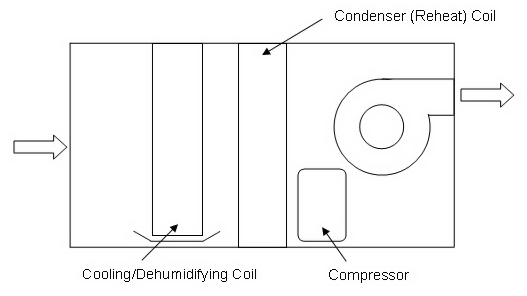
\includegraphics[width=0.9\textwidth, height=0.9\textheight, keepaspectratio=true]{media/image292.png}
\caption{Schematic of a mechanical dehumidifier \protect \label{fig:schematic-of-a-mechanical-dehumidifier}}
\end{figure}

The model has inputs for water removal, energy factor and air flow rate at rated conditions (26.7\si{\degreeCelsius}, 60\% RH). Curve objects must be specified to describe performance at off-rated conditions. A part-load cycling curve input must also be specified to account for inefficiencies due to cycling. Other inputs including minimum and maximum operating temperatures for dehumidifier operation, off-cycle parasitic load, and an input to direct the removed water to a storage tank.

The model assumes that this equipment dehumidifies and heats the air. If used in tandem with another system that cools and dehumidifies the zone air, then the zone dehumidifier should be specified as the lowest cooling priority in the \hyperref[zonehvacequipmentlist]{ZoneHVAC:EquipmentList} object for best control of zone temperature and humidity levels (e.g., if there are 3 pieces of equipment in \hyperref[zonehvacequipmentlist]{ZoneHVAC:EquipmentList}, then the zone dehumidifier should have Cooling Priority = 3). With this zone equipment prioritization, the other cooling and dehumidification system would operate first to meet the temperature setpoint (and possibly meet the high humidity setpoint as well). If additional dehumidification is needed, then the zone dehumidifier would operate. The sensible heat generated by the dehumidifier is carried over to the zone air heat balance for the next HVAC time step.

\subsubsection{Inputs}\label{inputs-12-021}

\paragraph{Field: Name}\label{field-name-12-014}

A unique user-assigned name for an instance of a zone DX dehumidifier unit. Any reference to this dehumidifier by another object will use this name.

\paragraph{Field: Availability Schedule Name}\label{field-availability-schedule-name-11-001}

This alpha field defines the name of the schedule (ref: Schedule) that denotes whether the dehumidifier operates during a given time period. A schedule value equal to 0 denotes that the dehumidifier will not operate for that time period. A value greater than 0 denotes that the dehumidifier is available to operate during that time period. If this field is left blank, the schedule has a value of 1 for all time periods.

\paragraph{Field: Air Inlet Node Name}\label{field-air-inlet-node-name-9-000}

This alpha field defines the name of the HVAC system node from which the dehumidifier draws its inlet air. This node name must be the name of a zone air exhaust node (ref. \hyperref[zonehvacequipmentconnections]{ZoneHVAC:EquipmentConnections}).

\paragraph{Field: Air Outlet Node Name}\label{field-air-outlet-node-name-9-001}

This alpha field defines the name of the HVAC system node to which the dehumidifier sends its outlet air. This node name must be the name of a zone air inlet node (ref. \hyperref[zonehvacequipmentconnections]{ZoneHVAC:EquipmentConnections}).

\paragraph{Field: Rated Water Removal}\label{field-rated-water-removal}

This numeric input is the full load water removal rate, in liters per day, at rated conditions (air entering the dehumidifier at 26.7\si{\degreeCelsius} {[}80°F{]} dry-bulb and 60\% relative humidity, and air flow rate as defined by field ``Rated Air Flow Rate'' below). This is a required input field and the entered value must be greater than zero.

\paragraph{Field: Rated Energy Factor}\label{field-rated-energy-factor}

This numeric input is the energy factor (liters of water removed per kWh of electricity consumed) at rated conditions (air entering the dehumidifier at 26.7\si{\degreeCelsius} {[}80°F{]} dry-bulb and 60\% relative humidity, and air flow rate as defined by field ``Rated Air Flow Rate'' below). This is a required input field and the entered value must be greater than zero.

\paragraph{Field: Rated Air Flow Rate}\label{field-rated-air-flow-rate-001}

This numeric input is the volumetric air flow rate through the dehumidifier, in m\(^{3}\) per second, at rated conditions (air entering the dehumidifier at 26.7\si{\degreeCelsius} {[}80°F{]} dry-bulb and 60\% relative humidity). This is a required input field and the entered value must be greater than zero.

\paragraph{Field: Water Removal Curve Name}\label{field-water-removal-curve-name}

This alpha field defines the name of a biquadratic performance curve (ref: Performance Curves) that parameterizes the variation of water removal as a function of the dry-bulb temperature (\si{\degreeCelsius}) and relative humidity (\%) of the air entering the dehumidifier. The output of this curve is multiplied by the Rated Water Removal to give the water removal of the dehumidifier at specific operating conditions (i.e., at temperatures and relative humidity levels different from the rating point conditions). The curve should be normalized to have the value of 1.0 at the rating point (air entering the dehumidifier at 26.7\si{\degreeCelsius} {[}80°F{]} dry-bulb and 60\% relative humidity, and air flow rate as defined by field ``Rated Air Flow Rate'' above).

\paragraph{Field: Energy Factor Curve Name}\label{field-energy-factor-curve-name}

This alpha field defines the name of a biquadratic performance curve (ref: Performance Curves) that parameterizes the variation of the energy factor as a function of the dry-bulb temperature (\si{\degreeCelsius}) and relative humidity (\%) of the air entering the dehumidifier. The output of this curve is multiplied by the Rated Energy Factor to give the energy factor of the dehumidifier at specific operating conditions (i.e., at temperatures and relative humidity levels different from the rating point conditions). The curve should be normalized to have the value of 1.0 at the rating point (air entering the dehumidifier at 26.7\si{\degreeCelsius} {[}80°F{]} dry-bulb and 60\% relative humidity, and air flow rate as defined by field ``Rated Air Flow Rate'' above).

\paragraph{Field: Part Load Fraction Correlation Curve Name}\label{field-part-load-fraction-correlation-curve-name-000}

This alpha field defines the name of a quadratic or cubic performance curve (ref: Performance Curves) that parameterizes the variation of electrical power input to the dehumidifier as a function of the part load ratio (PLR, defined as the water removal load to be met (kg/s) divided by the dehumidifier's water removal rate (kg/s) at the current operating conditions). The part load fraction (PLF) correlation accounts for efficiency losses due to compressor cycling.

The part load fraction correlation should be normalized to a value of 1.0 when the part load ratio equals 1.0 (i.e., no efficiency losses when the dehumidifier runs continuously for the simulation timestep). For PLR values between 0 and 1 (0 \textless{} = PLR \textless{} 1), the following rules apply:

0.7 \textless{} = PLF \textless{} = 1.0~~ and~~ PLF \textgreater{} = PLR

If PLF \textless{} 0.7 a warning message is issued, the program resets the PLF value to 0.7, and the simulation proceeds. The runtime fraction of the dehumidifier is defined as PLR/PLF. If PLF \textless{} PLR, then a warning message is issued and the runtime fraction of the dehumidifier is set to 1.0.

Mechanical dehumidifier typically have long runtimes with minimal compressor cycling. So, a typical part load fraction correlation might be:

~~~~~ PLF = 0.95 + 0.05(PLR)

If the user wishes to model no efficiency degradation due to compressor cycling, the part load fraction correlation should be defined as follows:

~~~~~ PLF = 1.0 + 0.0(PLR)

\paragraph{Field: Minimum Dry-Bulb Temperature for Dehumidifier Operation}\label{field-minimum-dry-bulb-temperature-for-dehumidifier-operation}

This numeric field defines the minimum inlet air dry-bulb temperature for dehumidifier operation. The dehumidifier will not operate if the inlet air temperature is below this value. This input value must be less than the Maximum Dry-Bulb Temperature for Dehumidifier Operation, and the default value is 10\si{\degreeCelsius}.

\paragraph{Field: Maximum Dry-Bulb Temperature for Dehumidifier Operation}\label{field-maximum-dry-bulb-temperature-for-dehumidifier-operation}

This numeric field defines the maximum inlet air dry-bulb temperature for dehumidifier operation. The dehumidifier will not operate if the inlet air temperature is above this value. This input value must be greater than the Minimum Dry-Bulb Temperature for Dehumidifier Operation, and the default value is 35\si{\degreeCelsius}.

\paragraph{Field: Off-Cycle Parasitic Electric Load}\label{field-off-cycle-parasitic-electric-load-001}

This numeric field contains the off-cycle parasitic electric power in Watts. This is the parasitic electric power consumed by controls or other electrical devices associated with the dehumidifier. This parasitic electric load is consumed whenever the dehumidifier is available to operate, but is not operating. The model assumed that this parasitic power contributes to heating the zone air (i.e., affects the zone air heat balance). The minimum value for this field is 0.0, and the default value is also 0.0 if this field is left blank.

\paragraph{Field: Condensate Collection Water Storage Tank Name}\label{field-condensate-collection-water-storage-tank-name-000}

This field is optional. It is used to specify where condensate from the dehumidifier is collected. If blank or omitted, then any water (condensate) removed is discarded. Enter the name of a Water Storage Tank (ref. \hyperref[waterusestorage]{WaterUse:Storage}) object defined elsewhere and the condensate will then be collected in that tank.

Following is an example input for a zone DX dehumidifier object. A \hyperref[zonecontrolhumidistat]{ZoneControl:Humidistat} object must also be specified for the zone to which the dehumidifier is connected (connect via a zone air exhaust node and a zone air inlet node, ref. \hyperref[zonehvacequipmentconnections]{ZoneHVAC:EquipmentConnections}).

\begin{lstlisting}

  ZoneHVAC:Dehumidifier:DX,
      North Zone Dehumidifier,  !- Name
      ON,                       !- Availability Schedule Name
      Zone3DehumidifierInlet,   !- Air Inlet Node Name
      Dehumidifier Outlet Node, !- Air Outlet Node Name
      50.16,                    !- Rated Water Removal {L/day} (106 pints/day)
      3.412,                    !- Rated Energy Factor {L/kWh} (7.21 pints/kWh)
      0.12036,                  !- Rated Air Flow Rate {m3/s} (255 cfm)
      ZoneDehumidWaterRemoval,  !- Water Removal Curve Name
      ZoneDehumidEnergyFactor,  !- Energy Factor Curve Name
      ZoneDehumidPLFFPLR,        !- Part Load Fraction Correlation Curve Name
      10.0,  !- Minimum Dry-Bulb Temperature for Compressor Operation {C}
      32.0,  !- Maximum Dry-Bulb Temperature for Compressor Operation {C}
      0.0;   !- Off Cycle Parasitic Electric Load {W}


    ZoneControl:Humidistat,
      Zone 3 Humidistat,       !- Name
      NORTH ZONE,              !- Zone Name
      Seasonal Relative Humidity Sch;  !- Relative Humidity Setpoint Schedule Name
\end{lstlisting}

\subsubsection{Outputs}\label{outputs-10-008}

\begin{itemize}
\item
  HVAC,Average,Zone Dehumidifier Sensible Heating Rate {[}W{]}
\item
  HVAC,Sum,Zone Dehumidifier Sensible Heating Energy {[}J{]}
\item
  HVAC,Average,Zone Dehumidifier Removed Water Mass Flow Rate {[}kg/s{]}
\item
  HVAC,Sum,Zone Dehumidifier Removed Water Mass {[}kg{]}
\item
  HVAC,Average,Zone Dehumidifier Electricity Rate {[}W{]}
\item
  HVAC,Sum,Zone Dehumidifier Electricity Energy {[}J{]}
\item
  HVAC,Average,Zone Dehumidifier Off Cycle Parasitic Electricity Rate {[}W{]}
\item
  HVAC,Sum,Zone Dehumidifier Off Cycle Parasitic Electricity Energy {[}J{]}
\item
  HVAC,Average,Zone Dehumidifier Part Load Ratio {[]}
\item
  HVAC,Average,Zone Dehumidifier Runtime Fraction {[]}
\item
  HVAC,Average,Zone Dehumidifier Outlet Air Temperature {[}\si{\degreeCelsius}{]}
\end{itemize}

If Condensate Collection Water Storage Tank Name is specified:

\begin{itemize}
\item
  HVAC,Average,Zone Dehumidifier Condensate Volume Flow Rate {[}m3/s{]}
\item
  HVAC,Sum,Zone Dehumidifier Condensate Volume {[}m3{]}
\end{itemize}

\paragraph{Zone Dehumidifier Sensible Heating Rate {[}W{]}}\label{zone-dehumidifier-sensible-heating-rate-w}

This output field is the sensible heating rate output of the dehumidifier in Watts. This is determined by the water removal rate, enthalpy of water evaporation, and the zone dehumidifier electric power. To reduce simulation time, this heating is carried over to the zone air heat balance for the next HVAC time step (i.e., it is reported here for the current time step but actually impacts the zone air heat balance on the following HVAC time step). This value is calculated for each HVAC system timestep, and the results are averaged for the timestep being reported.

\paragraph{Zone Dehumidifier Sensible Heating Energy {[}J{]}}\label{zone-dehumidifier-sensible-heating-energy-j}

This output field is the sensible heating output of the dehumidifier in Joules over the timestep being reported. This is determined by the water removal rate, enthalpy of water evaporation, and the zone dehumidifier electric power. To reduce simulation time, this heating is carried over to the zone air heat balance for the next HVAC time step (i.e., it is reported here for the current time step but actually impacts the zone air heat balance on the following HVAC time step). This value is calculated for each HVAC system timestep, and the results are summed for the timestep being reported.

\paragraph{Zone Dehumidifier Removed Water Mass Flow Rate {[}kg/s{]}}\label{zone-dehumidifier-removed-water-mass-flow-rate-kgs}

This output field is the water removal rate by the dehumidifier in kg/s. This value is calculated for each HVAC system timestep, and the results are averaged for the timestep being reported.

\paragraph{Zone Dehumidifier Removed Water Mass {[}kg{]}}\label{zone-dehumidifier-removed-water-mass-kg}

This output field is the water removed by the dehumidifier in kg. This value is calculated for each HVAC system timestep, and the results are summed for the timestep being reported.

\paragraph{Zone Dehumidifier Electricity Rate {[}W{]}}\label{zone-dehumidifier-electric-power-w}

\paragraph{Zone Dehumidifier Electricity Energy {[}J{]}}\label{zone-dehumidifier-electric-energy-j}

These outputs are the electric power and electric consumption of the dehumidifier for the time period being reported. They include all electricity used by the dehumidifier (including off-cycle electric parasitics). These values are calculated for each HVAC system timestep, and the results are averaged (power) or summed (consumption) for the timestep being reported. The electric consumption output is also added to a meter with Resource Type = Electricity, End Use Key = Cooling, Group Key = System (ref. Output:Meter objects).

\paragraph{Zone Dehumidifier Off Cycle Parasitic Electricity Rate {[}W{]}}\label{zone-dehumidifier-off-cycle-parasitic-electric-power-w}

\paragraph{Zone Dehumidifier Off Cycle Parasitic Electricity Energy {[}J{]}}\label{zone-dehumidifier-off-cycle-parasitic-electric-energy-j}

These outputs are the parasitic electric power and electric consumption for controls or other electrical devices associated with the dehumidifier. This parasitic electric load is consumed whenever the dehumidifier is available to operate, but is not operating. The model assumes that this parasitic power contributes to heating the zone air (i.e., affects the zone air heat balance). These outputs values are included in the Zone Dehumidifier Electric Power and Zone Dehumidifier Electricity Energy output variables.

\paragraph{Zone Dehumidifier Part Load Ratio {[]}}\label{zone-dehumidifier-part-load-ratio}

This output field is the part-load ratio for the dehumidifier. Part-load ratio is defined as the water removal load to be met (kg/s) divided by the dehumidifier's water removal rate (kg/s) at the current operating conditions. This value is calculated for each HVAC system timestep, and the results are averaged for the timestep being reported.

\paragraph{Zone Dehumidifier Runtime Fraction {[]}}\label{zone-dehumidifier-runtime-fraction}

This output field is the runtime fraction for the dehumidifier. This value is calculated for each HVAC system timestep, and the results are averaged for the timestep being reported.

\paragraph{Zone Dehumidifier Outlet Air Temperature {[}\si{\degreeCelsius}{]}}\label{zone-dehumidifier-outlet-air-temperature-c}

This output field is dry-bulb temperature of the air leaving the dehumidifier in Celsius. This value represents the dry-bulb temperature of the air leaving the dehumidifier when it is operating. For periods when the dehumidifier is not operating, the outlet air temperature is set equal to the inlet air temperature. This value is calculated for each HVAC system timestep, and the results are averaged for the timestep being reported.

\paragraph{Zone Dehumidifier Condensate Volume Flow Rate {[}m3/s{]}}\label{zone-dehumidifier-condensate-volume-flow-rate-m3s}

\paragraph{Zone Dehumidifier Condensate Volume {[}m3{]}}\label{zone-dehumidifier-condensate-volume-m3}

These outputs are the rate and volume of water removed as condensate by the dehumidifier. These reports only appear if a water storage tank is named in the input object. The condensate volume output is also added to a meter with Resource Type = OnSiteWater, End Use Key = Condensate, Group Key = System (ref. Output:Meter objects).

\subsection{ZoneHVAC:EnergyRecoveryVentilator}\label{zonehvacenergyrecoveryventilator}

The ZoneHVAC:EnergyRecoveryVentilator - stand alone energy recovery ventilator (ERV) is a single-zone HVAC component used for exhaust air heat recovery (Figure~\ref{fig:zonehvac-energyrecoveryventilator-compound}). This compound object consists of 3 required components: a generic air-to-air heat exchanger (see object Heat Exchanger:Air to Air:Generic), a supply air fan, and an exhaust air fan (see object \hyperref[fanonoff]{Fan:OnOff}).

An optional controller (see object \hyperref[zonehvacenergyrecoveryventilatorcontroller]{ZoneHVAC:EnergyRecoveryVentilator:Controller}) may be used to simulate economizer (free cooling) operation, modify air flow rates based on high indoor humidity, or simulate a ``push-button'' type economizer controller.

\begin{figure}[hbtp] % fig 115
\centering
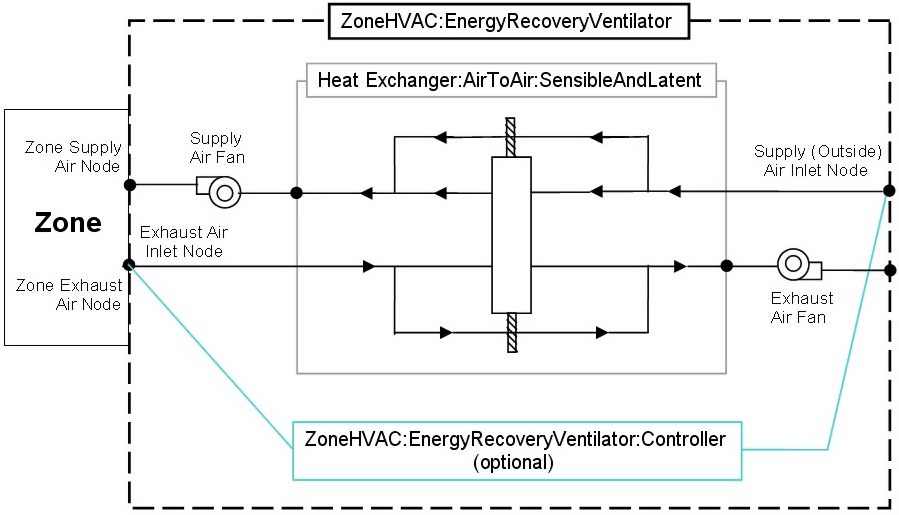
\includegraphics[width=0.9\textwidth, height=0.9\textheight, keepaspectratio=true]{media/image293.png}
\caption{ZoneHVAC:EnergyRecoveryVentilator compound object Schematic \protect \label{fig:zonehvac-energyrecoveryventilator-compound}}
\end{figure}

This compound object models the basic operation of supply and exhaust air fans and an air-to-air heat exchanger. The stand alone ERV operates whenever the unit is scheduled to be available (Availability schedule). The stand alone ERV object can be used in conjunction with an economizer feature whereby heat exchange is suspended whenever free cooling is available (i.e., air flow is fully bypassed around a fixed-plate heat exchanger or the rotation of a rotary heat exchanger is stopped). The economizer feature may also be activated based on a time-of-day schedule. Heat exchange is also suspended when air flow rates through the heat exchanger are modified in response to a zone humidistat. When an economizer is used in conjunction with high humidity control, high humidity control has the priority.

To model a stand alone ERV connected to a single zone, the input data file should include the following objects:

\begin{itemize}
\item
  ZoneHVAC:EnergyRecoveryVentilator
\item
  \hyperref[heatexchangerairtoairsensibleandlatent]{HeatExchanger:AirToAir:SensibleAndLatent}
\item
  \hyperref[fanonoff]{Fan:OnOff} (supply air)
\item
  \hyperref[fanonoff]{Fan:OnOff} (exhaust air)
\item
  \hyperref[zonehvacenergyrecoveryventilatorcontroller]{ZoneHVAC:EnergyRecoveryVentilator:Controller} (if economizer {[}free cooling{]} mode or high humidity control operation is desired)
\item
  \hyperref[zonecontrolhumidistat]{ZoneControl:Humidistat} (required for high humidity control option)
\item
  \hyperref[setpointmanagerscheduled]{SetpointManager:Scheduled} (if supply air outlet temperature control is used, Ref. Heat Exchanger:Air to Air:Generic for additional guidance)
\item
  \hyperref[zonehvacequipmentconnections]{ZoneHVAC:EquipmentConnections}
\item
  \hyperref[zonehvacequipmentlist]{ZoneHVAC:EquipmentList}
\item
  \hyperref[outdoorairnodelist]{OutdoorAir:NodeList}
\end{itemize}

A description of each input field for this compound object is provided below.

\subsubsection{Inputs}\label{inputs-13-018}

\paragraph{Field: Name}\label{field-name-13-012}

A unique user-assigned name for the stand alone ERV unit. Any reference to this unit by another object will use this name.

\paragraph{Field: Availability Schedule Name}\label{field-availability-schedule-name-12-001}

The name of the schedule (ref: Schedule) that denotes whether the unit can operate during a given time period. A schedule value greater than 0 (usually 1 is used) indicates that the unit can operate during the time period. A value less than or equal to 0 (usually 0 is used) denotes that the unit will not operate. If this field is left blank, the schedule has a value of 1 for all time periods.

\paragraph{Field: Heat Exchanger Name}\label{field-heat-exchanger-name-002}

The user-assigned name corresponding to the air-to-air heat exchanger used in this compound object. The only allowable type is:.

\hyperref[heatexchangerairtoairsensibleandlatent]{HeatExchanger:AirToAir:SensibleAndLatent}

\paragraph{Field: Supply Air Flow Rate}\label{field-supply-air-flow-rate-000}

The supply air flow rate through the ERV unit in cubic meters per second at standard temperature and pressure (dry air at 20\si{\degreeCelsius} drybulb). The program uses local barometric pressure to account for altitude using the equation for ``standard atmospheric'' pressure on p 6.1 of the ASHRAE 1997 HOF (SI edition) to initialize the air systems being simulated.

p = 101325*(1-2.25577E-05*Z)**5.2559

where p = pressure in Pa and Z = altitude in m

Note that this flow rate must be within the valid air flow range for the heat exchanger (ref: \hyperref[heatexchangerairtoairsensibleandlatent]{HeatExchanger:AirToAir:SensibleAndLatent} in the Engineering Document). In addition, this flow rate must be less than or equal to the supply fan air flow rate (\hyperref[fanonoff]{Fan:OnOff}). If the supply air flow rate is less than the exhaust air flow rate, the zone infiltration (ref: ZoneInfiltration) should be specified accordingly (the infiltration induced by imbalanced air flows is not accounted for automatically). The ERV supply air flow rate may also be autosized using the ventilation rate per floor area and/or ventilation rate per occupant fields below. When autosizing, the heat exchanger and fan air flow rates should also be autosized.

Note: The supply air inlet node specified in the generic heat exchanger object must be an outdoor air node (ref: \hyperref[outdoorairnode]{OutdoorAir:Node} and \hyperref[outdoorairnodelist]{OutdoorAir:NodeList}). The supply air outlet node specified in the generic heat exchanger object must be a zone air inlet node (ref: \hyperref[zonehvacequipmentconnections]{ZoneHVAC:EquipmentConnections}).

\paragraph{Field: Exhaust Air Flow Rate}\label{field-exhaust-air-flow-rate-1}

The exhaust air flow rate through the ERV unit in cubic meters per second at standard temperature and pressure (dry air at 20\si{\degreeCelsius} drybulb). The program uses local barometric pressure to account for altitude using the equation for ``standard atmospheric'' pressure on p 6.1 of the ASHRAE 1997 HOF (SI edition) to initialize the air systems being simulated.

p = 101325*(1-2.25577E-05*Z)**5.2559

where p = pressure in Pa and Z = altitude in m

Note that this flow rate must be within the valid air flow range for the heat exchanger (ref: \hyperref[heatexchangerairtoairsensibleandlatent]{HeatExchanger:AirToAir:SensibleAndLatent} in the Engineering Document). In addition, this flow rate must be less than or equal to the exhaust fan air flow rate (\hyperref[fanonoff]{Fan:OnOff}). If the exhaust air flow rate is greater than the supply air flow rate, the zone infiltration (ref: ZoneInfiltration) should be specified accordingly (the infiltration induced by imbalanced air flows is not accounted for automatically). The ERV exhaust air flow rate may also be autosized using the ventilation rate per floor area and/or ventilation rate per occupant fields below. When autosizing, the heat exchanger and fan air flow rates should also be autosized.

Note: The exhaust air inlet node specified in the generic heat exchanger object must be a zone air exhaust node (ref: \hyperref[zonehvacequipmentconnections]{ZoneHVAC:EquipmentConnections}).

\paragraph{Field: Supply Air Fan Name}\label{field-supply-air-fan-name-7}

The name of the supply air fan used in this object. Fan type must be \hyperref[fanonoff]{Fan:OnOff}.

\paragraph{Field: Exhaust Air Fan Name}\label{field-exhaust-air-fan-name}

The name of the exhaust air fan used in this object. Fan type must be \hyperref[fanonoff]{Fan:OnOff}.

\paragraph{Field: Controller Name}\label{field-controller-name}

This optional field specifies the name of the controller used by this compound component if economizer (free cooling) mode or high humidity control operation is desired. Controller type must be \hyperref[zonehvacenergyrecoveryventilatorcontroller]{ZoneHVAC:EnergyRecoveryVentilator:Controller}.

\paragraph{Field: Ventilation Rate per Unit Floor Area}\label{field-ventilation-rate-per-unit-floor-area}

This optional numeric field defines the ventilation rate per unit floor area in cubic meters per second per square meter. This field is only used when the supply and exhaust air flow rates are autosized.

\paragraph{Field: Ventilation Rate per Occupant}\label{field-ventilation-rate-per-occupant}

This optional numeric field defines the ventilation rate per occupant in cubic meters per second per occupant. This field is only used when the supply and exhaust air flow rates are autosized.

\paragraph{Field: Availability Manager List Name}\label{field-availability-manager-list-name-9}

This optional input field is the name of an \hyperref[availabilitymanagerassignmentlist]{AvailabilityManagerAssignmentList} object. An Availability Manager Assignment List is a list of Availability Managers giving both Availability Manager type and name. The availability managers in the list apply to this Stand Alone ERV~ object's fan. If the Stand Alone ERV is available (per the Availability Schedule Name input field above) and this input field has a valid availability manager assignment list name, then the availability managers in the list determine when and if the fan of this Stand Alone ERV~ object should be on or off.

Following is an example input for this compound object and associated objects that may be defined:

\begin{lstlisting}

ZoneHVAC:EnergyRecoveryVentilator,
      Stand Alone ERV 1,                        !- Stand alone ERV name
      FanAndCoilAvailSched,                     !- Availability schedule name
      OA Heat Recovery 1,                       !- Heat exchanger name
      0.05,                                     !- Supply air flow rate {m3/s}
      0.05,                                     !- Exhaust air flow rate {m3/s}
      Stand Alone ERV Supply Fan,               !- Supply air fan name
      Stand Alone ERV Exhaust Fan,              !- Exhaust air fan name
      ERV OA Controller 1;                      !- ERV controller name


  OutdoorAir:NodeLine,
      OutsideAirInletNodes;       !- 1st Node name or node list name


  NodeList,
      OutsideAirInletNodes,       !- Node List Name
      ERV Outdoor air Inlet Node; !- Node_ID_1




  ZoneHVAC:EquipmentConnections,
      RESISTIVE ZONE,      !- Zone Name
      Zone1Equipment,      !- List Name: Zone Equipment
      Zone1Inlets,         !- List Name: Zone Inlet Nodes
      Zone1Exhausts,       !- List Name: Zone Exhaust Nodes
      Zone 1 Node,         !- Zone Air Node Name
      Zone 1 Outlet Node;  !- Zone Return Air Node Name


  ZoneHVAC:EquipmentList,
      Zone1Equipment,                          !-Name
      ZoneHVAC:EnergyRecoveryVentilator,  !- KEY--Zone Equipment Type 1
      Stand Alone ERV 1,                       !- Type Name 1
      1,                                       !- Cooling Priority
      1;                                       !- Heating Priority


  NodeList,
      Zone1Inlets,                             !- Node List Name
      Stand Alone ERV Supply Fan Outlet Node;  !- Node_ID_1


  NodeList,
      Zone1Exhausts,         !- Node List Name
      Zone 1 Exhaust Node;   !- Node_ID_1


  ZoneHVAC:EnergyRecoveryVentilator:Controller,
      ERV OA Controller 1,           !- ERV controller name
      0.05,                          !- Outdoor air flow rate {m3/s}
      19.,                           !- Temperature high limit {C}
      14.,                           !- Temperature low limit {C}
      0.0,                           !- Enthalpy high limit {J/kg}
      NoExhaustAirTemperatureLimit,     !- Exhaust air temperature limit
      NoExhaustAirEnthalpyLimit; !- Exhaust air enthalpy limit




  HeatExchanger:AirToAir:SensibleAndLatent,
      OA Heat Recovery 1,            !- Heat exchanger name
      FanAndCoilAvailSched,          !- Availability schedule name
      0.05,                          !- Nominal supply air flow rate {m3/s}
      .76,                           !- Sensible effectiveness at 100% airflow heating condition
      .68,                           !- Latent effectiveness at 100% airflow heating condition
      .81,                           !- Sensible effectiveness at 75% airflow heating condition
      .73,                           !- Latent effectiveness at 75% airflow heating condition
      .76,                           !- Sensible effectiveness at 100% airflow cooling condition
      .68,                           !- Latent effectiveness at 100% airflow cooling condition
      .81,                           !- Sensible effectiveness at 75% airflow cooling condition
      .73,                           !- Latent effectiveness at 75% airflow cooling condition
      ERV Outdoor air Inlet Node,    !- Supply air inlet node name
      Heat Recovery Outlet Node,     !- Supply air outlet node name
      Zone 1 Exhaust Node,           !- Exhaust air inlet node name
      Heat Recovery Secondary Outlet Node,  !- Exhaust air outlet node name
      50.0,                          !- Nominal electric power {W}
      Yes,                           !- Supply air outlet temperature control
      Rotary,                        !- Heat exchanger type
      MinimumExhaustTemperature,   !- Frost control type
      1.7;                           !- Threshold temperature




  Fan:OnOff,
      Stand Alone ERV Supply Fan,               !- Fan Name
      FanAndCoilAvailSched,                     !- Availability Schedule Name
      0.5,                                      !- Fan Total Efficiency
      75.0,                                     !- Delta Pressure {Pa}
      0.05,                                     !- Max Flow Rate {m3/s}
      0.9,                                      !- Motor Efficiency
      1.0,                                      !- Motor In Airstream Fraction
      Heat Recovery Outlet Node,                !- Fan_Inlet_Node
      Stand Alone ERV Supply Fan Outlet Node;   !- Fan_Outlet_Node


  Fan:OnOff,
      Stand Alone ERV Exhaust Fan,              !- Fan Name
      FanAndCoilAvailSched,                     !- Availability Schedule Name
      0.5,                                      !- Fan Total Efficiency
      75.0,                                     !- Delta Pressure {Pa}
      0.05,                                     !- Max Flow Rate {m3/s}
      0.9,                                      !- Motor Efficiency
      1.0,                                      !- Motor In Airstream Fraction
      Heat Recovery Secondary Outlet Node,      !- Fan_Inlet_Node
      Stand Alone ERV Exhaust Fan Outlet Node;  !- Fan_Outlet_Node


  SetpointManager:Scheduled,
      Heat Exhchanger Supply Air Temp Manager,  !- Name
      Temperature,  !- Control variable
      Heat Exchanger Supply Air Temp Sch,  !- Schedule Name
      Heat Exchanger Supply Air Nodes;     !- Name of the set point Node List


  NodeList,
      Heat Exchanger Supply Air Nodes,  !- Node List Name
      Heat Recovery Outlet Node;        !- Node_ID_1
\end{lstlisting}

\subsubsection{Outputs}\label{outputs-11-006}

\begin{itemize}
\item
  HVAC,Average,Zone Ventilator Electricity Rate {[}W{]}
\item
  HVAC,Sum,Zone Ventilator Electricity Energy {[}J{]}
\item
  HVAC,Average,Zone Ventilator Total Cooling Rate {[}W{]}
\item
  HVAC,Sum,Zone Ventilator Total Cooling Energy {[}J{]}
\item
  HVAC,Average,Zone Ventilator Total Heating Rate {[}W{]}
\item
  HVAC,Sum,Zone Ventilator Total Heating Energy {[}J{]}
\item
  HVAC,Average,Zone Ventilator Sensible Cooling Rate {[}W{]}
\item
  HVAC,Sum,Zone Ventilator Sensible Cooling Energy {[}J{]}
\item
  HVAC,Average,Zone Ventilator Sensible Heating Rate {[}W{]}
\item
  HVAC,Sum,Zone Ventilator Sensible Heating Energy {[}J{]}
\item
  HVAC,Average,Zone Ventilator Latent Cooling Rate {[}W{]}
\item
  HVAC,Sum,Zone Ventilator Latent Cooling Energy {[}J{]}
\item
  HVAC,Average,Zone Ventilator Latent Heating Rate {[}W{]}
\item
  HVAC,Sum,Zone Ventilator Latent Heating Energy {[}J{]}
\item
  HVAC,Average,Zone Ventilator Supply Fan Availability Status {[]}
\end{itemize}

\paragraph{Zone Ventilator Electricity Rate {[}W{]}}\label{zone-ventilator-electric-power-w}

This output field is the electric consumption rate of the stand alone energy recovery ventilator in Watts. This rate includes the electric consumption by the supply air fan, exhaust air fan and the generic air-to-air heat exchanger.

\paragraph{Zone Ventilator Electricity Energy {[}J{]}}\label{zone-ventilator-electric-energy-j}

This output field is the electric consumption of the stand alone energy recovery ventilator in Joules for the timestep being reported. This value includes the electric consumption by the supply air fan, exhaust air fan and the generic air-to-air heat exchanger.

\paragraph{Zone Ventilator Total Cooling Rate {[}W{]}}\label{zone-ventilator-total-cooling-rate-w}

This output field is the total (enthalpy) heat extraction rate of the stand alone energy recovery ventilator from the zone in Watts. This value is calculated using the supply air outlet mass flow rate, and the enthalpy difference of the supply outlet and exhaust inlet air streams. This value is calculated for each HVAC system timestep being simulated, and the results (enthalpy extraction only) are averaged for the timestep being reported.

\paragraph{Zone Ventilator Total Cooling Energy {[}J{]}}\label{zone-ventilator-total-cooling-energy-j}

This output field is the total (enthalpy) heat extraction of the stand alone energy recovery ventilator from the zone in Joules over the timestep being reported. This value is calculated using the supply air outlet mass flow rate, the enthalpy difference of the supply outlet and exhaust inlet air streams, and the HVAC system timestep. This value is calculated for each HVAC system timestep being simulated, and the results (enthalpy extraction only) are summed for the timestep being reported.

\paragraph{Zone Ventilator Total Heating Rate {[}W{]}}\label{zone-ventilator-total-heating-rate-w}

This output field is the total (enthalpy) heat addition rate of the stand alone energy recovery ventilator to the zone in Watts. This value is calculated using the supply air outlet mass flow rate, and the enthalpy difference of the supply outlet and exhaust inlet air streams. This value is calculated for each HVAC system timestep being simulated, and the results (enthalpy addition only) are averaged for the timestep being reported.

\paragraph{Zone Ventilator Total Heating Energy {[}J{]}}\label{zone-ventilator-total-heating-energy-j}

This output field is the total (enthalpy) heat addition of the stand alone energy recovery ventilator to the zone in Joules over the timestep being reported. This value is calculated using the supply air outlet mass flow rate, the enthalpy difference of the supply outlet and exhaust inlet air streams, and the HVAC system timestep. This value is calculated for each HVAC system timestep being simulated, and the results (enthalpy addition only) are summed for the timestep being reported.

\paragraph{Zone Ventilator Sensible Cooling Rate {[}W{]}}\label{zone-ventilator-sensible-cooling-rate-w}

This output is the moist air sensible heat extraction rate of the stand alone energy recovery ventilator from the zone in Watts. This value is calculated using the supply air outlet mass flow rate, and the enthalpy difference of the supply outlet and exhaust inlet air streams at a constant humidity ratio. This value is calculated for each HVAC system timestep being simulated, and the results (cooling only) are averaged for the timestep being reported.

\paragraph{Zone Ventilator Sensible Cooling Energy {[}J{]}}\label{zone-ventilator-sensible-cooling-energy-j}

This output is the moist air sensible heat extraction of the stand alone energy recovery ventilator from the zone in Joules over the timestep being reported. This value is calculated using the supply air outlet mass flow rate, the enthalpy difference of the supply outlet and exhaust inlet air streams at a constant humidity ratio, and the HVAC system timestep. This value is calculated for each HVAC system timestep being simulated, and the results (cooling only) are summed for the timestep being reported.

\paragraph{Zone Ventilator Sensible Heating Rate {[}W{]}}\label{zone-ventilator-sensible-heating-rate-w}

This output is the sensible heat addition rate of the stand alone energy recovery ventilator to the zone in Watts. This value is calculated using the supply air outlet mass flow rate, and the enthalpy difference of the supply outlet and exhaust inlet air streams at a constant humidity ratio. This value is calculated for each HVAC system timestep being simulated, and the results (heating only) are averaged for the timestep being reported.

\paragraph{Zone Ventilator Sensible Heating Energy {[}J{]}}\label{zone-ventilator-sensible-heating-energy-j}

This output is the sensible heat addition of the stand alone energy recovery ventilator to the zone in Joules over the timestep being reported. This value is calculated using the supply air outlet mass flow rate, the enthalpy difference of the supply outlet and exhaust inlet air streams at a constant humidity ratio, and the HVAC system timestep. This value is calculated for each HVAC system timestep being simulated, and the results (heating only) are summed for the timestep being reported.

\paragraph{Zone Ventilator Latent Cooling Rate {[}W{]}}\label{zone-ventilator-latent-cooling-rate-w}

This output is the latent heat extraction (dehumidification) rate of the stand alone energy recovery ventilator from the zone in Watts. This value is calculated as the difference between the total energy rate and the sensible energy rate provided by the stand alone ERV. This value is calculated for each HVAC system timestep being simulated, and the results (latent heat extraction only) are averaged for the timestep being reported.

\paragraph{Zone Ventilator Latent Cooling Energy {[}J{]}}\label{zone-ventilator-latent-cooling-energy-j}

This output is the latent heat extraction (dehumidification) of the stand alone energy recovery ventilator from the zone in Joules over the timestep being reported. This value is calculated as the difference between the total energy delivered to the zone and the sensible energy delivered to the zone by the stand alone ERV. This value is calculated for each HVAC system timestep being simulated, and the results (latent heat extraction only) are summed for the timestep being reported.

\paragraph{Zone Ventilator Latent Heating Rate {[}W{]}}\label{zone-ventilator-latent-heating-rate-w}

This output is the latent heat addition (humidification) rate of the stand alone energy recovery ventilator to the zone in Watts. This value is calculated as the difference between the total energy rate and the sensible energy rate provided by the stand alone ERV. This value is calculated for each HVAC system timestep being simulated, and the results (latent heat addition only) are averaged for the timestep being reported.

\paragraph{Zone Ventilator Latent Heating Energy {[}J{]}}\label{zone-ventilator-latent-heating-energy-j}

This output is the latent heat addition (humidification) of the stand alone energy recovery ventilator to the zone in Joules over the timestep being reported. This value is calculated as the difference between the total energy delivered to the zone and the sensible energy delivered to the zone by the stand alone ERV. This value is calculated for each HVAC system timestep being simulated, and the results (latent heat addition only) are summed for the timestep being reported.

\paragraph{Zone Ventilator Supply Fan Availability Status {[]}}\label{zone-ventilator-supply-fan-availability-status}

This is the availability status of the Stand Alone ERV~ fan. This status flag is a result of the calculations made by the Availability Manager(s) listed in an AvailabilityManagerAssignmentList object and/or calculations made by Hybrid Ventilation Manager object. The AvailabilityManagerAssignmentList is an optional input in the Stand Alone ERV~ object. When a single availability manager is used in an Availability Manager Assignment List, this is also the availability status reported by the specific availability manager (Ref. AvailabilityManager:* Outputs). For multiple availability managers in an Availability Manager Assignment List (with or without Hybrid Ventilation Manager), rules to determine fan availability status are described in the section `Group -- System Availability Managers'. The control status outputs are represented using integers 0 through 3. These integers represent NoAction (0), ForceOff (1), CycleOn (2), and CycleOnZoneFansOnly (3). Since the status output is averaged, the output result may not correspond to the values described here when output variable frequencies other than detailed are used. Use the ``detailed'' reporting frequency (Ref. Output:Variable object) to view the availability status at each simulation timestep.

\subsection{ZoneHVAC:TerminalUnit:VariableRefrigerantFlow}\label{zonehvacterminalunitvariablerefrigerantflow}

Terminal units with variable refrigerant flow compound HVAC object are used exclusively with variable refrigerant flow (VRF) air conditioning systems (Ref. \hyperref[airconditionervariablerefrigerantflow]{AirConditioner:VariableRefrigerantFlow} objects). The VRF terminal unit may be used as zone, air loop or outside air system equipment. The VRF terminal unit compound object contains an optional outdoor air mixer, a DX cooling coil, a DX heating coil, a supply fan (optional for air loop and outdoor air system equipment), and an optional supplemental heating coil object.

\begin{callout}
Note: The terminal unit may be used in the air loop and/or outdoor air system, however, at this time only constant flow (or limited variation within the limits allowed for DX coils) through the unit is allowed. Using a wide range of outdoor air flow rates will cause the DX coil model to fail. For example, if the minimum outdoor air flow rate is allowed to fall near 0, the DX coil model will calculate very low, even very negative, coil outlet temperatures. This can cause psychrometric warnings to occur and cause the simulation to end prematurely.
\end{callout}

For zone equipment the terminal units are connected to a zone using the inlet and exhaust node names specified in a \hyperref[zonehvacequipmentconnections]{ZoneHVAC:EquipmentConnections} object. The zone exhaust node has the same name as the terminal unit air inlet node. The zone inlet node has the same name as the terminal unit air outlet node. The zone terminal unit is also listed in a zone's equipment list and will typically be the first equipment operating for both cooling and heating (i.e., Sequence = 1 in the \hyperref[zonehvacequipmentlist]{ZoneHVAC:EquipmentList}). Other ZoneHVAC equipment may be used in the same zone and should be sequenced to operate after the zone terminal units (i.e., sequence = 2 or higher).

For air loop equipment and outdoor air system equipment the VRF terminal unit inlet and outlet nodes define the location of the system in the air loop and outdoor air system. The node names must define the path of the air stream in order from the beginning of the air loop or outdoor air system to the outlet of that system.

This VRF terminal unit can be controlled based on a load or set point. When the system is used as zone equipment load control is always used. When the VRF terminal unit is used in an air loop and the control zone name or thermostat location is specified, the system is controlled based on zone load. If the control zone name or thermostat location is not specified the VRF terminal unit will be controlled based on termninal unit or coil outlet node set point temperature. When set point based control is used the node temperature set points may be placed at the outlet of the terminal unit or at individual coil outlet nodes. If the VRF terminal unit is used in an air loop's outdoor air system, control is always based on a termninal unit or coil outlet node temperature set point.

The terminal units operate to satisfy a heating or cooling load in a zone based on a zone thermostat temperature set point. A direct-expansion (DX) cooling and/or DX heating coil is specified depending on the operating mode required. Both a DX cooling and DX heating coil will typically be installed in the terminal unit, however only one may be used if desired. An optional supplemental heating coil can also be added to the terminal unit to provide additional heating when the main DX heating coil could not meet the entire heating load of a zone during cold outdoor conditions. The Supplemental Heating Coil Object Type must be \hyperref[coilheatingelectric]{Coil:Heating:Electric}, \hyperref[coilheatinggas-000]{Coil:Heating:Fuel}, \hyperref[coilheatingwater]{Coil:Heating:Water}, or \hyperref[coilheatingsteam]{Coil:Heating:Steam}. Outdoor ventilation air is modeled with the use of an optional outside air mixer object. Outside air may be provided to the zone only when the coil is operating or can be supplied continuously even when the coil is not operating.

A supply air fan can be modeled as either draw through or blow through. The supply air fan is required for zone equipment and optional for air loop and outdoor air system equipment. The Supply Air Fan Object Type must be \hyperref[fansystemmodel]{Fan:SystemModel}, \hyperref[fanonoff]{Fan:OnOff}, or \hyperref[fanconstantvolume]{Fan:ConstantVolume} if \hyperref[airconditionervariablerefrigerantflow]{AirConditioner:VariableRefrigerantFlow} is used to model the VRF outdoor unit. The Supply Air Fan Object Type must be \hyperref[fansystemmodel]{Fan:SystemModel} or \hyperref[fanvariablevolume]{Fan:VariableVolume} if AirConditioner:VariableRefrigerantFlow:\-FluidTemperatureControl or AirConditioner:VariableRefrigerantFlow:\-FluidTemperatureControl:HR is used to model the VRF outdoor unit.

\subsubsection{Inputs}\label{inputs-14-018}

\paragraph{Field: Zone Terminal Unit Name}\label{field-zone-terminal-unit-name}

This alpha field defines a unique user-assigned name for an instance of a variable refrigerant flow zone terminal unit. Any reference to this terminal unit by another object will use this name. The zone terminal unit name must be specified in a \hyperref[zoneterminalunitlist]{ZoneTerminalUnitList} object to connect this terminal unit to an \hyperref[airconditionervariablerefrigerantflow]{AirConditioner:VariableRefrigerantFlow} object.

\paragraph{Field: Availability Schedule Name}\label{field-availability-schedule-name-13-001}

This alpha field defines the name of the schedule (ref: Schedule) that denotes whether the terminal unit operates during a given time period. A schedule value equal to 0 denotes that the terminal unit must be off for that time period. A value greater than 0 denotes that the terminal unit is available to operate during that time period. This schedule may be used to completely disable the terminal unit as required. If this field is left blank, the schedule has a value of 1 for all time periods.

\paragraph{Field: Terminal Unit Air Inlet Node Name}\label{field-terminal-unit-air-inlet-node-name}

This alpha field defines the name of the terminal unit air inlet node. This node name should be the same as a zone exhaust node (ref: \hyperref[zonehvacequipmentconnections]{ZoneHVAC:EquipmentConnections}).

\paragraph{Field: Terminal Unit Air Outlet Node Name}\label{field-terminal-unit-air-outlet-node-name}

This alpha field defines the name of the terminal unit air outlet node. This node name should be the same as a zone inlet node (ref: \hyperref[zonehvacequipmentconnections]{ZoneHVAC:EquipmentConnections}).

\paragraph{Field: Cooling Supply Air Flow Rate}\label{field-cooling-supply-air-flow-rate-3-001}

This numeric field defines the terminal unit's operating volumetric air flow rate in cubic meters per second. This volumetric air flow rate is used when the terminal unit is operating in cooling mode.

\paragraph{Field: No Cooling Supply Air Flow Rate}\label{field-no-cooling-supply-air-flow-rate-000}

This numeric field defines the terminal unit's operating volumetric air flow rate in cubic meters per second. This volumetric air flow rate is used when the terminal unit's cooling coil is not operating and the previous mode was cooling.

\paragraph{Field: Heating Supply Air Flow Rate}\label{field-heating-supply-air-flow-rate-3-001}

This numeric field defines the terminal unit's operating volumetric air flow rate in cubic meters per second. This volumetric air flow rate is used when the terminal unit is operating in heating mode.

\paragraph{Field: No Heating Supply Air Flow Rate}\label{field-no-heating-supply-air-flow-rate-000}

This numeric field defines the terminal unit's operating volumetric air flow rate in cubic meters per second. This volumetric air flow rate is used when the terminal unit's heating coil is not operating and the previous mode was heating.

\paragraph{Field: Cooling Outdoor Air Flow Rate}\label{field-cooling-outdoor-air-flow-rate-3}

This numeric field defines the outdoor air volumetric air flow rate in cubic meters per second. This volumetric air flow rate is used when the terminal unit is operating in cooling mode. This input field is set to zero flow when the VRF terminal unit is connected to an \textit{\hyperref[airterminalsingleductmixer]{AirTerminal:SingleDuct:Mixer}} object.

\paragraph{Field: Heating Outdoor Air Flow Rate}\label{field-heating-outdoor-air-flow-rate-3}

This numeric field defines the outdoor air volumetric air flow rate in cubic meters per second. This volumetric air flow rate is used when the terminal unit is operating in heating mode. This input field is set to zero flow when the VRF terminal unit is connected to an \textit{\hyperref[airterminalsingleductmixer]{AirTerminal:SingleDuct:Mixer}} object.

\paragraph{Field: No Load Outdoor Air Flow Rate}\label{field-no-load-outdoor-air-flow-rate-2}

This numeric field defines the outdoor air volumetric air flow rate in cubic meters per second. This volumetric air flow rate is used when the terminal unit is not operating in cooling or heating mode. This input field is set to zero flow when the VRF terminal unit is connected to an \textit{\hyperref[airterminalsingleductmixer]{AirTerminal:SingleDuct:Mixer}} object.

\paragraph{Field: Supply Air Fan Operating Mode Schedule Name}\label{field-supply-air-fan-operating-mode-schedule-name-7}

This alpha field defines the name of the supply air fan operating mode schedule. Schedule values equal to 0 denote cycling fan/cycling coil operation. All other schedule values denote constant fan/cycling coil operation.

\paragraph{Field: Supply Air Fan Placement}\label{field-supply-air-fan-placement-000}

This alpha field has two choices: \textit{BlowThrough} or \textit{DrawThrough}. If this field is left blank, the default is blow through.

The first choice stands for ``blow through fan''. This means that the unit consists of a fan followed by the DX coils. The fan ``blows through'' the cooling and heating coils. If an outside air mixer is used, the fan inlet connects to the outdoor air mixer's mixed air node. If an outdoor air mixer is not used, the fan inlet connects to the zone exhaust node. For this configuration, the fan outlet always connects to the DX cooling coil inlet node (or if a DX cooling coil is not used, the DX heating coil inlet node).

The second choice stands for ``draw through fan''. This means that the unit consists of the DX coil(s) followed by a fan. The fan ``draws air through'' the DX coil(s). In this case the fan inlet always connects to the DX heating coil outlet node (or if a DX heating coil is not use, the DX cooling coil outlet node) and the fan outlet node always connects to the zone inlet node.

\paragraph{Field: Supply Air Fan Object Type}\label{field-supply-air-fan-object-type-8}

This choice field contains the identifying type of supply air fan specified for the furnace. Fan type must be \textit{\hyperref[fanonoff]{Fan:OnOff}}, \textit{\hyperref[fanconstantvolume]{Fan:ConstantVolume}}, \textit{\hyperref[fansystemmodel]{Fan:SystemModel}} or \textit{\hyperref[fanvariablevolume]{Fan:VariableVolume}}. The Supply Air Fan Object Type must be \hyperref[fansystemmodel]{Fan:SystemModel}, \hyperref[fanonoff]{Fan:OnOff}, or \hyperref[fanconstantvolume]{Fan:ConstantVolume} if \hyperref[airconditionervariablerefrigerantflow]{AirConditioner:VariableRefrigerantFlow} is used to model the VRF outdoor unit. The Supply Air Fan Object Type must be \hyperref[fansystemmodel]{Fan:SystemModel} or \hyperref[fanvariablevolume]{Fan:VariableVolume} if AirConditioner:VariableRefrigerantFlow:\-FluidTemperatureControl or AirConditioner:VariableRefrigerantFlow:\-FluidTemperatureControl:HR is used to model the VRF outdoor unit.

\hyperref[fanconstantvolume]{Fan:ConstantVolume} is used when the Supply Air Fan Operating Mode Schedule values are never 0 and the fan operates continuously. \hyperref[fanonoff]{Fan:OnOff} is used when the fan cycles on and off with the cooling or heating coil (i.e.~Supply Air Fan Operating Mode Schedule values are at times 0). The \hyperref[fansystemmodel]{Fan:SystemModel} may be used to model either of these fan operating characteristics.

This field may be left blank when the VRF terminal unit is used as air loop or outdoor air system equipment.

\paragraph{Field: Supply Air Fan Object Name}\label{field-supply-air-fan-object-name}

This alpha field defines the name of the terminal unit's supply air fan. This field may be left blank when the VRF terminal unit is used as air loop or outdoor air system equipment.

\paragraph{Field: Outdoor Air Mixer Object Type}

This alpha field contains the identifying type of outdoor air mixer specified for the terminal unit. Outdoor air mixer type must be \textit{\hyperref[outdoorairmixer]{OutdoorAir:Mixer}}. This input field should be left blank when the VRF terminal unit is connected to an \textit{\hyperref[airterminalsingleductmixer]{AirTerminal:SingleDuct:Mixer}} object. If this field is left blank, an outdoor air mixer is not simulated. If the VRF terminal unit is used as air loop equipment and this terminal unit's outdoor air flow rates are autosized then the autosized flow rates will be set to 0 when an outdoor air system is used in the air loop (ref \textit{\hyperref[airloophvacoutdoorairsystem]{AirloopHVAC:OutdoorAirSystem}}).

\paragraph{Field: Outdoor Air Mixer Object Name}\label{field-outdoor-air-mixer-object-name}

This alpha field defines the name of the terminal unit's outdoor air mixer. This input field should be left blank when the VRF terminal unit is connected to an \textit{\hyperref[airterminalsingleductmixer]{AirTerminal:SingleDuct:Mixer}} object. If this field is left blank, an outdoor air mixer is not simulated.

\paragraph{Field: DX Cooling Coil Object Type}\label{field-dx-cooling-coil-object-type}

This choice field contains the identifying type of the terminal unit's DX cooling coil. The only valid DX cooling coil type is \textit{\hyperref[coilcoolingdxvariablerefrigerantflow]{Coil:Cooling:DX:VariableRefrigerantFlow}}. This field should be left blank when a DX cooling coil is not simulated.

\paragraph{Field: DX Cooling Coil Name}\label{field-dx-cooling-coil-name-1}

This alpha field defines the name of the terminal unit's DX cooling coil. If this field is left blank, a DX cooling coil is not simulated.

\paragraph{Field: DX Heating Coil Object Type}\label{field-dx-heating-coil-object-type}

This choice field contains the identifying type of the terminal unit's DX heating coil. The only valid DX heating coil type is \textit{\hyperref[coilheatingdxvariablerefrigerantflow]{Coil:Heating:DX:VariableRefrigerantFlow}}. This field should be left blank when a DX heating coil is not simulated.

\paragraph{Field: DX Heating Coil Object Name}\label{field-dx-heating-coil-object-name}

This alpha field defines the name of the terminal unit's DX heating coil. This field should be left blank when a DX heating coil is not simulated.

\paragraph{Field: Zone Terminal Unit On Parasitic Electric Energy Use}\label{field-zone-terminal-unit-on-parasitic-electric-energy-use-000}

This numeric field defines the parasitic electrical energy use of the zone terminal unit when either terminal unit coil is operating. When in cooling mode, this electric energy use is reported in a zone terminal unit cooling electric consumption output variable. When in heating mode, this electric energy use is reported in a zone terminal unit heating electric consumption output variable.

\paragraph{Field: Zone Terminal Unit Off Parasitic Electric Energy Use}\label{field-zone-terminal-unit-off-parasitic-electric-energy-use-000}

This numeric field defines the parasitic electrical energy use of the zone terminal unit when the terminal unit coil(s) is not operating. When the previous mode was cooling, this electric energy use is reported in a zone terminal unit cooling electric consumption output variable. When the previous mode was heating, this electric energy use is reported in a zone terminal unit heating electric consumption output variable.

\paragraph{Field: Rated Total Heating Capacity Sizing Ratio}\label{field-rated-total-heating-capacity-sizing-ratio-000}

This numeric field defines the ratio of the heating coil to cooling coil size when autosizing is used. The model assumes that when used, this value will be greater than 1. This field supersedes the Rated Total Heating Capacity Sizing Ratio entered in the \hyperref[airconditionervariablerefrigerantflow]{AirConditioner:VariableRefrigerantFlow} object. If this field is left blank, the value entered in the parent object is used for sizing. If neither field is used, the sizing ratio is assumed to be 1.

\paragraph{Field: Availability Manager List Name}\label{field-availability-manager-list-name-10}

This optional input field is the name of an \hyperref[availabilitymanagerassignmentlist]{AvailabilityManagerAssignmentList} object. An Availability Manager Assignment List is a list of Availability Managers giving both Availability Manager type and name. The availability managers in the list apply to this Zone Terminal Unit object's fan. If the Zone Terminal Unit is available (per the Availability Schedule Name input field above) and this input field has a valid availability manager assignment list name, then the availability managers in the list determine when and if the fan of this Zone Terminal Unit object should be on or off.

\paragraph{Field: Design Specification ZoneHVAC Sizing Object Name}\label{field-design-specification-zonehvac-sizing-object-name-9}

This optional input field is the name of a \hyperref[designspecificationzonehvacsizing]{DesignSpecification:ZoneHVAC:Sizing} object. The name must correspond to unique name of a \hyperref[designspecificationzonehvacsizing]{DesignSpecification:ZoneHVAC:Sizing} object. A Design Sepcification Zone HVAC Sizing object defines scalable sizing methods for sizing input fields such as Cooling Supply Air Flow Rate in this VRF terminal unit zone HVAC object. The scaled Supply Air Flow Rate in turn is used to size cooling and heating capacity of the unit.

\paragraph{Field: Supplemental Heating Coil Object Type}\label{field-supplemental-heating-coil-object-type-2-000}

This alpha field defines the type of supplemental heating coil to be used by this VRF terminal unit. The input requirements for these heating coil objects are described elsewhere in this document. The hot water and steam heating coils require specifying plant loop, branches, and connector objects to support the heating coils, and are placed on the demand side of the plantloop. The hot water flow modulation through the supplemental heating coil does not require additional controller or Controller:WaterCoil object. The parent object (VRF terminal unit) itself provides the “controller” function of modulating water flow. Supplemental Heating Coil Object Type must be \hyperref[coilheatingelectric]{Coil:Heating:Electric}, \hyperref[coilheatinggas-000]{Coil:Heating:Fuel}, \hyperref[coilheatingwater]{Coil:Heating:Water}, or \hyperref[coilheatingsteam]{Coil:Heating:Steam}.

\paragraph{Field: Supplemental Heating Coil Name}\label{field-supplemental-heating-coil-name-2-000}

This alpha field defines the name of the supplemental heating coil used by this VRF terminal unit, and this name should match the name specified in the corresponding heating coil object.

\paragraph{Field: Maximum Supply Air Temperature from Supplemental Heater}\label{field-maximum-supply-air-temperature-from-supplemental-heater-2-000}

This numeric field defines the maximum supply air temperature in degrees Celsius leaving the VRF terminal unit supplemental heater coil. The supplemental heater will be controlled so that its supply air temperature does not exceed this value. This field is autosizable. If this input field is left blank, the value defaults to autosize.

\paragraph{Field: Maximum Outdoor Dry-Bulb Temperature for Supplemental Heater Operation}\label{field-maximum-outdoor-dry-bulb-temperature-for-supplemental-heater-operation-2-000}

This numeric field defines the maximum outdoor dry-bulb temperature in degrees Celsius for this VRF terminal unit supplemental heating coil operation. The supplemental heater will not operate when the outdoor dry-bulb temperature is above this value. The maximum value must be less than or equal to 21\si{\degreeCelsius}. If this field is left blank, the default value of 21\si{\degreeCelsius} will be used.

\paragraph{Field: Controlling Zone or Thermostat Location}\label{controlling-zone-or-thermostat-location-2-110}

This alpha field is only used when this VRF terminal unit is used as air loop equipment with load based operational control. When the terminal unit is used in an air loop and this terminal unit is load controlled, this zone's thermostat will control operation. When this terminal unit is used in an air loop and is set point controlled, this field must be blank (i.e., when the controlling zone name is present the system will be load controlled).

Following is an example input for a ZoneHVAC:TerminalUnit:VariableRefrigerantFlow object.

\begin{lstlisting}

ZoneHVAC:TerminalUnit:VariableRefrigerantFlow,
  Zone 1 TU,               !- Zone Terminal Unit Name
  TU Availability Schedule,!- Terminal Unit Availability schedule
  TU1 Inlet Node,          !- Terminal Unit Air Inlet Node Name
  TU1 Outlet Node,         !- Terminal Unit Air Outlet Node Name
  0.005,                   !- Cooling Supply Air Flow Rate {m3/s}
  0,                       !- No Cooling Supply Air Flow Rate {m3/s}
  0.005,                   !- Heating Supply Air Flow Rate {m3/s}
  0,                       !- No Heating Supply Air Flow Rate {m3/s}
  0.001,                   !- Cooling Outdoor Air Flow Rate
  0.001,                   !- Heating Outdoor Air Flow Rate
  0,                       !- No Load Outdoor Air Flow Rate
  TU1 Fan Op Schedule,     !- Supply Air Fan Operating Mode Schedule Name
  drawthrough,             !- Supply Air Fan placement
  Fan:ConstantVolume,      !- Supply Air Fan Object Type
  TU1 SA Fan,              !- Supply Air Fan Object Name
  OutdoorAir:Mixer,        !- Outside Air Mixer Object Type
  TU1 OA Mixer,            !- Outside Air Mixer Object Name
  COIL:Cooling:DX:VariableRefrigerantFlow,  !- Cooling Coil Object Type
  TU1 VRF DX Cooling Coil, !- Cooling Coil Object Name
  COIL:Heating:DX:VariableRefrigerantFlow,  !- Heating Coil Object Type
  TU1 VRF DX Heating Coil, !- Heating Coil Object Name
  30,                      !- Zone Terminal Unit On Parasitic Electric Energy Use {W}
  20,                      !- Zone Terminal Unit Off Parasitic Electric Energy Use {W}
  ,                        !- Rated Total Heating Capacity Sizing Ratio {W/W}
  ,                        !- Availability Manager List Name
  ,                        !- Design Specification ZoneHVAC Sizing Object Name
  Coil:Heating:Electric,   !- Supplemental Heating Coil Object Type
  TU1 Supp Heating Coil,   !- Supplemental Heating Coil Name
  autosize,                !- Maximum Supply Air Temperature from Supplemental Heater
  ,                        !- Maximum Outdoor Dry-Bulb Temperature for Supplemental Heater Operation
  ;                        !- Controlling Zone or Thermostat Location
\end{lstlisting}

\subsubsection{Outputs}\label{outputs-12-006}

\begin{itemize}
\item
  HVAC,Average,Zone VRF Air Terminal Total Cooling Rate {[}W{]}
\item
  HVAC,Sum, Zone VRF Air Terminal Total Cooling Energy {[}J{]}
\item
  HVAC,Average, Zone VRF Air Terminal Sensible Cooling Rate {[}W{]}
\item
  HVAC,Sum, Zone VRF Air Terminal Sensible Cooling Energy {[}J{]}
\item
  HVAC,Average, Zone VRF Air Terminal Latent Cooling Rate {[}W{]}
\item
  HVAC,Sum, Zone VRF Air Terminal Latent Cooling Energy {[}J{]}
\item
  HVAC,Average,Zone VRF Air Terminal Total Heating Rate {[}W{]}
\item
  HVAC,Sum, Zone VRF Air Terminal Total Heating Energy {[}J{]}
\item
  HVAC,Average, Zone VRF Air Terminal Sensible Heating Rate {[}W{]}
\item
  HVAC,Sum, Zone VRF Air Terminal Sensible Heating Energy {[}J{]}
\item
  HVAC,Average, Zone VRF Air Terminal Latent Heating Rate {[}W{]}
\item
  HVAC,Sum, Zone VRF Air Terminal Latent Heating Energy {[}J{]}
\item
  HVAC,Average, Zone VRF Air Terminal Cooling Electricity Rate {[}W{]}
\item
  HVAC,Sum, Zone VRF Air Terminal Cooling Electricity Energy {[}J{]}
\item
  HVAC,Average,Zone VRF Air Terminal Heating Electricity Rate {[}W{]}
\item
  HVAC,Sum,Zone VRF Air Terminal Heating Electricity Energy {[}J{]}
\item
  HVAC,Average, Zone VRF Air Terminal Fan Availability Status {[]}
\end{itemize}

\paragraph{Zone VRF Air Terminal Total Cooling Rate {[}W{]}}\label{zone-vrf-air-terminal-total-cooling-rate-w}

This field is the total (sensible and latent) cooling rate output of the terminal unit in Watts. This is determined by terminal unit inlet and outlet air conditions and the air mass flow rate through the unit. This value describes the total energy rate delivered to the zone.

\paragraph{Zone VRF Air Terminal Total Cooling Energy {[}J{]}}\label{zone-vrf-air-terminal-total-cooling-energy-j}

This is the total (sensible plus latent) cooling output of the terminal unit in Joules over the time step being reported. This is determined by the terminal unit inlet and outlet air conditions and the air mass flow rate through the unit. This value describes the total cooling energy delivered to the zone.

\paragraph{Zone VRF Air Terminal Sensible Cooling Rate {[}W{]}}\label{zone-vrf-air-terminal-sensible-cooling-rate-w}

This output is the moist air sensible cooling rate output of the terminal unit in Watts. This is determined by enthalpy difference between the inlet and outlet air temperature at a constant humidity ratio, using the minimum of the inlet and outlet air node humidity ratios, and the air mass flow rate through the unit. This value describes the sensible cooling energy rate delivered to the zone.

\paragraph{Zone VRF Air Terminal Sensible Cooling Energy {[}J{]}}\label{zone-vrf-air-terminal-sensible-cooling-energy-j}

This is the moist air sensible cooling output of the terminal unit in Joules for the time step being reported. This is determined by enthalpy difference between the inlet and outlet air temperature at a constant humidity ratio, using the minimum of the inlet and outlet air node humidity ratios, and the air mass flow rate through the unit. This value describes the sensible cooling energy delivered to the zone.

\paragraph{Zone VRF Air Terminal Latent Cooling Rate {[}W{]}}\label{zone-vrf-air-terminal-latent-cooling-rate-w}

This is the latent cooling rate output of the terminal unit in Watts. This is determined by the inlet and outlet air humidity ratios and the air mass flow rate through the unit. This value describes the latent cooling energy rate delivered to the zone.

\paragraph{Zone VRF Air Terminal Latent Cooling Energy {[}J{]}}\label{zone-vrf-air-terminal-latent-cooling-energy-j}

This is the latent cooling output of the terminal unit in Joules for the time step being reported. This is determined by the inlet and outlet air humidity ratios and the air mass flow rate through the unit. This value describes the latent cooling energy delivered to the zone.

\paragraph{Zone VRF Air Terminal Total Heating Rate {[}W{]}}\label{zone-vrf-air-terminal-total-heating-rate-w}

This field is the total enthalpic heating rate output of the terminal unit in Watts. This is determined by the terminal unit inlet and outlet air conditions and the air mass flow rate through the unit. This value describes the total heating energy rate delivered to the zone.

\paragraph{Zone VRF Air Terminal Total Heating Energy {[}J{]}}\label{zone-vrf-air-terminal-total-heating-energy-j}

This is the total enthalpic heating output of the terminal unit in Joules over the time step being reported. This is determined by the terminal unit inlet and outlet air conditions and the air mass flow rate through the unit. This value describes the total heating energy delivered to the zone.

\paragraph{Zone VRF Air Terminal Sensible Heating Rate {[}W{]}}\label{zone-vrf-air-terminal-sensible-heating-rate-w}

This output is the moist air sensible heating rate output of the terminal unit in Watts. This is determined by enthalpy difference between the inlet and outlet air temperature at a constant humidity ratio, using the minimum of the inlet and outlet air node humidity ratios, and the air mass flow rate through the unit. This value describes the sensible heating energy rate delivered to the zone.

\paragraph{Zone VRF Air Terminal Sensible Heating Energy {[}J{]}}\label{zone-vrf-air-terminal-sensible-heating-energy-j}

This is the moist air sensible heating output of the terminal unit in Joules for the time step being reported. This is determined by enthalpy difference between the inlet and outlet air temperature at a constant humidity ratio, using the minimum of the inlet and outlet air node humidity ratios, and the air mass flow rate through the unit. This value describes the sensible heating energy delivered to the zone.

\paragraph{Zone VRF Air Terminal Latent Heating Rate {[}W{]}}\label{zone-vrf-air-terminal-latent-heating-rate-w}

This is the latent heating rate output of the terminal unit in Watts. This is determined by the inlet and outlet air specific humidity ratios and the air mass flow rate through the unit. This value describes the latent heating energy rate delivered to the zone.

\paragraph{Zone VRF Air Terminal Latent Heating Energy {[}J{]}}\label{zone-vrf-air-terminal-latent-heating-energy-j}

This is the latent heating output of the terminal unit in Joules for the time step being reported. This is determined by the inlet and outlet air specific humidity ratios and the air mass flow rate through the unit. This value describes the latent heating energy delivered to the zone.

\paragraph{Zone VRF Air Terminal Cooling Electricity Rate {[}W{]}}\label{zone-vrf-air-terminal-cooling-electric-powerw}

This output field is the parasitic electricity consumption rate of the zone terminal unit in Watts. The consumption rate includes parasitic electricity used by the zone terminal unit's transformers, controls, or other electricity consuming devices. This value is calculated for each HVAC system time step being simulated, and the results are averaged for the time step being reported. The terminal unit parasitic on and off electricity is reported in this cooling output variable when the unit operates in cooling mode or the most recent operation was for cooling.

\paragraph{Zone VRF Air Terminal Cooling Electricity Energy {[}J{]}}\label{zone-vrf-air-terminal-cooling-electric-energy-j}

This output field is the electricity consumption of the zone terminal unit in Joules for the time period being reported. The consumption includes parasitic electricity used by the zone terminal unit's transformers, controls, or other electricity consuming devices. This value is calculated for each HVAC system time step being simulated, and the results are summed for the time step being reported. The terminal unit parasitic on and off electricity consumption is reported in this cooling output variable when the unit operates in cooling mode or the most recent operation was for cooling. This output is also added to a meter with Resource Type = Electricity, End Use Key = Cooling, Group Key = System (ref. Output:Meter objects).

\paragraph{Zone VRF Air Terminal Heating Electricity Rate {[}W{]}}\label{zone-vrf-air-terminal-heating-electric-powerw}

This output field is the parasitic electricity consumption rate of the zone terminal unit in Watts. The consumption rate includes parasitic electricity used by the zone terminal unit's transformers, controls, or other electricity consuming devices. This value is calculated for each HVAC system time step being simulated, and the results are averaged for the time step being reported. The terminal unit parasitic on and off electricity is reported in this heating output variable when the unit operates in heating mode or the most recent operation was for heating.

\paragraph{Zone VRF Air Terminal Heating Electricity Energy {[}J{]}}\label{zone-vrf-air-terminal-heating-electric-energy-j}

This output field is the electricity consumption of the zone terminal unit in Joules for the time period being reported. The consumption includes parasitic electricity used by the zone terminal unit's transformers, controls, or other electricity consuming devices. This value is calculated for each HVAC system time step being simulated, and the results are summed for the time step being reported. The terminal unit parasitic on and off electricity consumption is reported in this heating output variable when the unit operates in heating mode or the most recent operation was for heating. This output is also added to a meter with Resource Type = Electricity, End Use Key = Heating, Group Key = System (ref. Output:Meter objects).

\paragraph{Zone VRF Air Terminal Fan Availability Status {[]}}\label{zone-vrf-air-terminal-fan-availability-status}

This is the availability status of the Zone Terminal Unit fan. This status flag is a result of the calculations made by the Availability Manager(s) listed in an AvailabilityManagerAssignmentList object and/or calculations made by Hybrid Ventilation Manager object. The AvailabilityManagerAssignmentList is an optional input in the Zone Terminal Unit object. When a single availability manager is used in an Availability Manager Assignment List, this is also the availability status reported by the specific availability manager (Ref. AvailabilityManager:* Outputs). For multiple availability managers in an Availability Manager Assignment List along with Hybrid Ventilation Manager, rules to determine fan availability status are described in the section `Group -- System Availability Managers'. The control status outputs are represented using integers 0 through 3. These integers represent NoAction (0), ForceOff (1), CycleOn (2), and CycleOnZoneFansOnly (3). Since the status output is averaged, the output result may not correspond to the values described here when output variable frequencies other than detailed are used. Use the ``detailed'' reporting frequency (Ref. Output:Variable object) to view the availability status at each simulation timestep.

\subsection{ZoneHVAC:HybridUnitaryHVAC}\label{zonehvac-hybridunitaryhvac}

ZoneHVAC:Hybrid UnitaryHVAC is a black-box model for packaged forced air equipment with multiple discrete operating modes. Generally, a ''hybrid`` is any system that exhibits both continuous and discrete dynamic behavior – a system that can both flow (as could be described by a differential equation) and jump (as must be described by distinct modes). Equipment in this category may utilize a wide variety technologies including, but not limited to: indirect evaporative cooling, desiccant dehumidification, heat recovery, vapor compression, adsorption, or ventilation cooling. Each hybrid system packages multiple technologies into a single integrated system. There are a multitude of unique hybrid system architectures, and each unique system may have numerous unique operating modes.

\begin{figure}[hbtp]
\centering
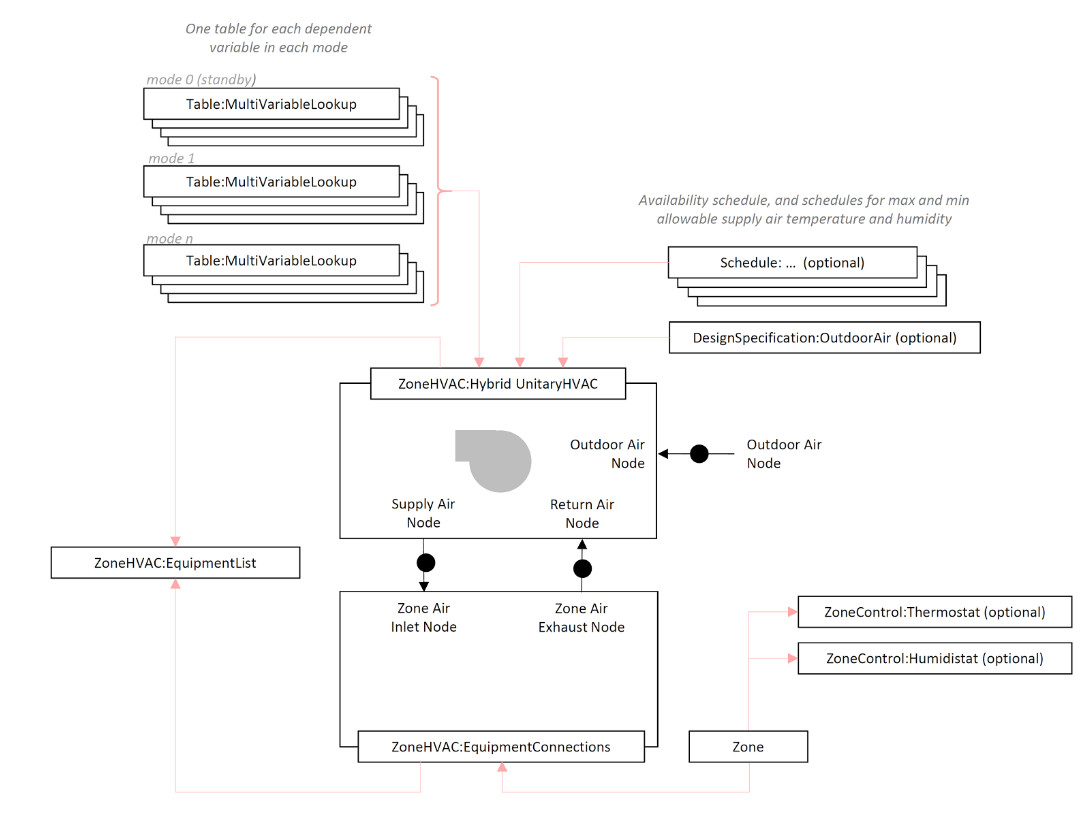
\includegraphics[width=0.9\textwidth, height=0.9\textheight, keepaspectratio=true]{media/hybrid001.jpg}
\caption{Schematic of object links for ZoneHVAC:HybridUnitaryHVAC \protect \label{fig:hybrid001}}
\end{figure}

ZoneHVAC:HybridUnitaryHVAC is a black-box model designed to allow empirical representation of a wide variety of hybrid unitary systems. The model does not require information about internal system architecture, however it requires extensive data to describe the performance of a product in every operating mode. The model is intended for packed forced air equipment and can represent unitary systems that consume electricity, water, and up to two additional fuel types.

Uncontrolled independent variables include outdoor and indoor air temperature and humidity ratio. Controlled independent variables include: operating mode, supply air flow rate, outdoor air fraction, and part runtime fraction. Dependent variables include supply air temperature, supply air humidity, electricity use, fuel uses, water use, fan electricity use, and external static pressure. Empirical data tables (see \hyperref[tablelookup]{Table:Lookup}) are required to map each dependent variable in each discrete operating mode. The model can accommodate up to 26 discrete operating modes, including a standby mode. Each mode is limited to operate within independently specified ranges of indoor and outdoor psychrometric conditions.  The standby mode is not limited by either indoor or outdoor psychrometric conditions.

\begin{figure}[hbtp]
\centering
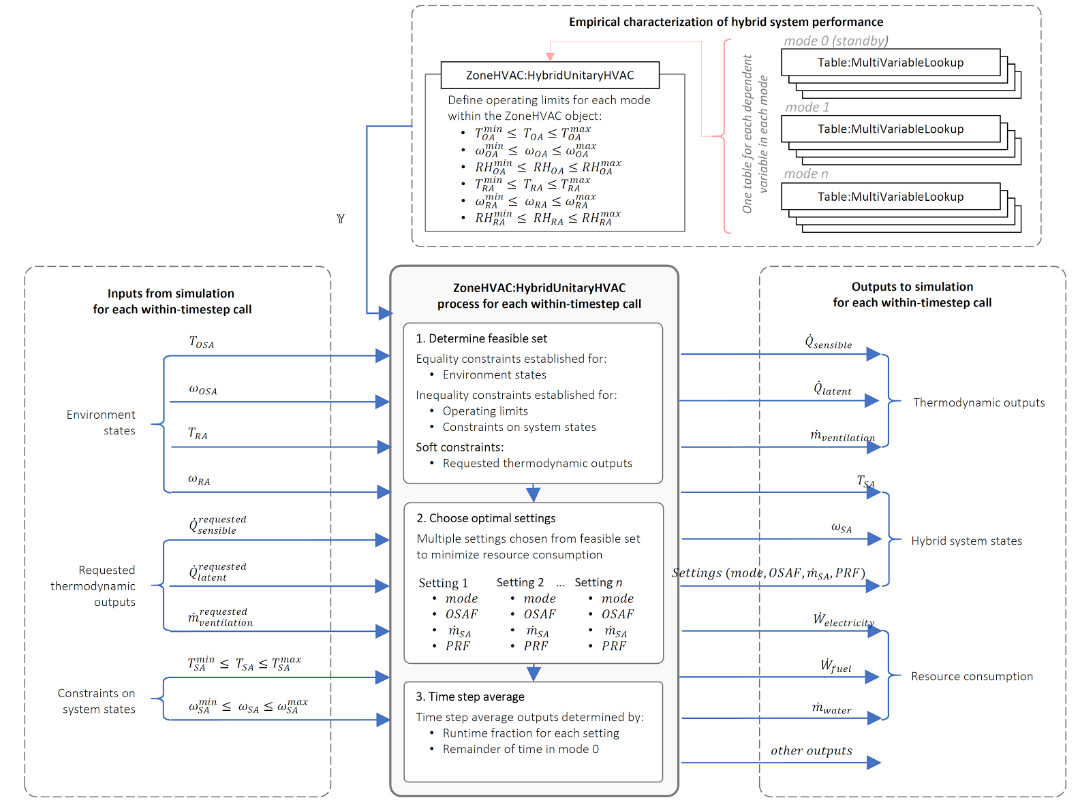
\includegraphics[width=0.9\textwidth, height=0.9\textheight, keepaspectratio=true]{media/hybrid002.jpg}
\caption{Schematic explanation of the architecture and function of ZoneHVAC:HybridUnitaryHVAC \protect \label{fig:hybrid002}}
\end{figure}

ZoneHVAC:HybridUnitaryHVAC is structured as a constrained optimization problem – in each time step the model will choose one or more combinations of the controlled independent variables so as to best provide the predicted sensible load, the predicted latent load, and the scheduled zone ventilation requirement, with the least amount of resource consumption.

A setting is defined as any unique combination of mode, outdoor air fraction, and supply air flow rate. The system may operate with multiple settings in each time step. The portion of each time step spent in a setting is described as the part runtime fraction for that setting. During any time step that the combination of settings can satisfy all of the soft constraints with part runtime fractions that sum to less than one, the system will operate in a standby mode (Mode 0) for the remainder of the timestep. If no combination of settings will satisfy all of  the soft constraints the system will choose the combination of settings that most nearly satisfies all soft constraints. If the indoor and outdoor psychrometric conditions are beyond the constraints that limit each operating mode, or if no setting will satisfy all constraints on supply air temperature and absolute humidity, the system will operate in standby mode (Mode 0).

\subsubsection{Inputs}

\paragraph{Field: Name}

This alpha input field specifies a unique user-assigned name for one ZoneHVAC:HybridUnitaryHVAC unit. Any reference to this unit by another object will use this name. The name must be specified in a \hyperref[zonehvacequipmentlist]{ZoneHVAC:EquipmentList} object to connect this unit to a zone.

\paragraph{Field: Availability Schedule Name}
This alpha input field specifies the name of the schedule (ref: Group – Schedules) that specifies when the ZoneHVAC:HybridUnitaryHVAC unit can operate. A schedule value greater than 0 means the unit can be available. A schedule value equal to zero means the unit cannot operate. Availability of the unit is governed by the availability schedule and by availability managers. The availability schedule may be used to completely disable the unit.  If this field is blank, the unit can always be available. If the unit is available but there is no sensible load, no latent load, and no need for ventilation, the unit will operate in a standby mode (mode 0).

\paragraph{Field: Availability Manager List Name}
This optional alpha input field is the name of an \hyperref[availabilitymanagerassignmentlist]{AvailabilityManagerAssignmentList} object.
(ref: Group - Air Distribution, \hyperref[availabilitymanagerassignmentlist]{AvailabilityManagerAssignmentList}, and Group - System Availability Managers). Availability of the unit is governed by the availability schedule and by availability managers specified in the list named here. If the unit is available but there is no sensible load, no latent load, and no need for ventilation, the unit will operate in a standby mode (mode 0).

\paragraph{Field: Minimum Supply Air Temperature Schedule Name}
This optional alpha input field specifies the name of the schedule (ref: Group – Schedules) that specifies the minimum supply air temperature allowed in each time step. Values in this schedule are used as a constraint in choosing the feasible settings for supply air flow rate and outdoor air fraction in each operating mode. If this field is blank, no minimum is imposed.

\paragraph{Field: Maximum Supply Air Temperature Schedule Name}
This optional alpha input field specifies the name of the schedule (ref: Group – Schedules) that specifies the maximum supply air temperature allowed in each time step. Values in this schedule are used as a constraint in choosing the feasible settings for supply air flow rate and outdoor air fraction in each operating mode. If this field is blank, no maximum is imposed.

\paragraph{Field: Minimum Supply Air Humidity Ratio Schedule Name}
This optional alpha input field specifies the name of the schedule (ref: Group – Schedules) that specifies the minimum supply air humidity ratio allowed in each time step. Values in this schedule are used as a constraint in choosing the feasible settings for supply air flow rate and outdoor air fraction in each operating mode. If this field is blank, no minimum is imposed.

\paragraph{Field: Maximum Supply Air Humidity Ratio Schedule Name}
This optional alpha input field specifies the name of the schedule (ref: Group – Schedules) that specifies the maximum supply air humidity raio allowed in each time step. Values in this schedule are used as a constraint in choosing the feasible settings for supply air flow rate and outdoor air fraction in each operating mode. If this field is blank, no maximum is imposed.

\paragraph{Field: Method to Choose Controlled Inputs and Part Runtime Fraction}
This alpha input field specifies the method that will be used to choose operating mode(s), supply air flow rate(s), outdoor air fraction(s) and part runtime fraction(s) in each time step. The only valid choices are ''Automatic`` and ''User Defined``, ''Automatic`` chooses the controlled independent variables to minimize resource use within each time step, subject to constraints, while best satisfying zone sensible loads, latent loads, and the scheduled ventilation rate. ''User Defined`` indicates that the user will provide a custom control sequence, using Energy Management System objects or other means, to choose the controlled independent variables and determine system outputs in each time step.

\paragraph{Field: Return Air Node Name}
This alpha input field specifies the name of the HVAC system node from which the hybrid unit draws return air. This node name must also be specified as a zone return air node in a \hyperref[zonehvacequipmentconnections]{ZoneHVAC:EquipmentConnections} object. It may also be included in \hyperref[nodelist]{NodeList} object that is specified as a zone return air node in a \hyperref[zonehvacequipmentconnections]{ZoneHVAC:EquipmentConnections} object. (Ref. Group - Zone Equipment \hyperref[zonehvacequipmentconnections]{ZoneHVAC:EquipmentConnections} and Group - Node-Branch Management \hyperref[nodelist]{NodeList}).

\paragraph{Field: Outdoor Air Node Name}
This alpha input field specifies the name of the HVAC system node from which the hybrid unit draws outdoor air. This node name must also be specified in an \hyperref[outdoorairnode]{OutdoorAir:Node} or \hyperref[outdoorairnodelist]{OutdoorAir:NodeList} object. (Ref. Group - Node-Branch Management \hyperref[outdoorairnode]{OutdoorAir:Node} and \hyperref[outdoorairnodelist]{OutdoorAir:NodeList}).

\paragraph{Field: Supply Air Node Name}
This alpha input field specifies the name of the HVAC system node to which the hybrid unit sends supply air. This node name must also be specified as zone inlet node in a \hyperref[zonehvacequipmentconnections]{ZoneHVAC:EquipmentConnections} object. It may also be included in \hyperref[nodelist]{NodeList} object that is specified as a zone inlet node in a \hyperref[zonehvacequipmentconnections]{ZoneHVAC:EquipmentConnections} object. (Ref. Group - Zone Equipment \hyperref[zonehvacequipmentconnections]{ZoneHVAC:EquipmentConnections} and Group - Node-Branch Management \hyperref[nodelist]{NodeList}).

\paragraph{Field: Relief Node Name}
This optional alpha input field specifies the name of an HVAC system node which can extract air from the zone to balance the air supplied to the zone by the unit. This node name would match the name of a zone exhaust air node.

\paragraph{Field: System Maximum Supply Air Volume Flow Rate}
This numeric input field specifies the maximum standard density supply air volume flow rate among all operating modes. The field allows custom resizing of the hybrid unit. The values specified in each \hyperref[tablelookup]{Table:Lookup} object associated with a hybrid unit represent performance data for a specific product of a particular size, but the value output from each \hyperref[tablelookup]{Table:Lookup} object is augmented by a normalization reference (Ref: Group - Performance Tables \hyperref[tablelookup]{Table:Lookup}). The normalization reference specified for all \hyperref[tablelookup]{Table:Lookup} objects associated with a hybrid unit should be the maximum supply air mass flow rate for the real hybrid unit that was used to create the performance data included in each table object. The value in this field is used to rescale the normalized values output from tables for extensive dependent variables. If the standard density supply air volume flow rate input to this field is equivalent to the system maximum supply air mass flow rate used as the normalization reference – given appropriate unit conversions – then the resulting output from the model will exactly match the original performance data specified in each table. If the value in this field is larger or smaller, the values for extensive dependent variables will be scaled proportionally. The values of intensive dependent variables are rescaled by the normalization reference value, so will always match the original performance data specified in each table object. The value in this field should be specified as standard density volume flow rate. Standard density in EnergyPlus corresponds to dry air at 20\si{\degreeCelsius} drybulb, and 101,325 Pa.

\paragraph{Field: External Static Pressure at System Maximum Supply Air Flow Rate}
This optional numeric input field specifies the external static pressure at the system maximum supply air flow rate specified in the previous field. Fan affinity laws are used to scale supply fan power from the scenario used to create the performance data included in each \hyperref[tablelookup]{Table:Lookup} object, to a scenario that corresponds to the value specified in this field. The result is also used to adjust the system electric power accordingly. If this field is blank, the supply fan power is not scaled from the values specified in lookup tables.

\paragraph{Field: Fan Heat Included in Lookup Tables}
This alpha field specifies if the fan heat gain was taken into account in the lookup tables specified for each mode. Valid choices are \textbf{\emph{Yes}} and \textbf{\emph{No}}. If No, the fan heat is calculated based on the fan power and the next two fields specify the location and fraction of the fan heat gain to the air stream, otherwise the fan heat gain is not calculated.

\paragraph{Field: Fan Heat Gain Location}
This optional alpha field specifies the location that the fan heat gain should be applied if not included in the lookup tables. Valid choices include: \textbf{\emph{MixedAirStream}} and \textbf{\emph{SupplyAirStream}}. MixedAirStream is upstream of the cooling medium while SupplyAirStream is downstream of the cooling medium.

\paragraph{Field: Fan Heat Gain in Airstream Fraction}
This optional numeric field is the fraction of the fan heat that is added to the air stream if not included in the lookup tables. A value of 0 means that the fan heat is completely outside the air stream. A value of 1 means that all of the fan heat loss will go into the air stream and act to cause a temperature rise. Must be between 0 and 1. The default is 1.0.

\paragraph{Field: Scaling Factor}
This optional numeric field scales all extensive dependent variables including: supply air mass flow rate, electricity use, fuel uses, and water use. The value in this field acts together with the value in field System Maximum Standard Density Supply Air Volume Flow Rate to allow custom resizing of the hybrid unit.

\paragraph{Field: Minimum Time Between Mode Change}
This numeric field specifies the minimum time that must pass before the hybrid unit can change mode. If the value in this field is larger than each timestep, the mode selected in one time step will persist in later time steps until the minimum time between mode change is satisfied. If the value in this field is smaller than each timestep, it will determine the minimum part runtime fraction allowed for any mode. Supply air mass flow rate and outdoor air fraction within a mode are not subject to minimum runtime and may change in every time step, or with any part runtime fraction. Mode 0 does not have a minimum time. If this field is blank, the default minimum time between mode change is 10 minutes.

\paragraph{Field: First Fuel Type}
This alpha field specifies the fuel type associated with the \hyperref[tablelookup]{Table:Lookup} object specified in field ''System Electric Power Power Lookup Table``. Valid choices include: None, Electricity, NaturalGas, Propane, FuelOilNo1, FuelOilNo2, Diesel, Gasoline, Coal, OtherFuel1, OtherFuel2, Steam, \hyperref[districtheating]{DistrictHeating} and \hyperref[districtcooling]{DistrictCooling}. If this field is blank, the default first fuel type is Electricity.

\paragraph{Field: Second Fuel Type}
This alpha field specifies the fuel type associated with the \hyperref[tablelookup]{Table:Lookup} object specified in field ''System Second Fuel Consumption Lookup Table``. Valid choices include: None, Electricity, NaturalGas, Propane, FuelOilNo1, FuelOilNo2, Diesel, Gasoline, Coal, OtherFuel1, OtherFuel2, Steam, \hyperref[districtheating]{DistrictHeating} and \hyperref[districtcooling]{DistrictCooling}. If this field is blank, the default second fuel type is None.

\paragraph{Field: Third Fuel Type}
This alpha field specifies the fuel type associated with the \hyperref[tablelookup]{Table:Lookup} object specified in field ''System Third Fuel Consumption Lookup Table``. Valid choices include: None, Electricity, NaturalGas, Propane, FuelOilNo1, FuelOilNo2, Diesel, Gasoline, Coal, OtherFuel1, OtherFuel2, Steam, \hyperref[districtheating]{DistrictHeating} and \hyperref[districtcooling]{DistrictCooling}. If this field is blank, the default second fuel type is None.

\paragraph{Field: Objective Function to Minimize}
In each time step ZoneHVAC:HybridUnitaryHVAC will choose one or more combinations of the controlled independent variables, subject to constraints, so as to best satisfy sensible load, latent load, and scheduled ventilation with the least amount of resource consumption. This alpha field specifies which resource will be minimized by the optimization.  Valid choices include: Electricity Use, Second Fuel Use, Third Fuel Use, and Water Use.  If this field is blank, the objective function will minimize electricity use.


\paragraph{Field: Design Specification Outdoor Air Object Name}
This alpha field specifies the name of a \hyperref[designspecificationoutdoorair]{DesignSpecification:OutdoorAir} object which specifies the a schedule for the required standard density volume of outdoor air. If this field is blank, the system may still supply outdoor air, if it is capable, when doing so is the most efficient way to satisfy other constraints.

\paragraph{Field: Mode 0 Name}
This alpha input field specifies a unique user-assigned descriptive name for Mode 0. Mode 0 describes performance when the hybrid unit is in standby. Mode 0 is usually characterized by electricity use for controls and crankcase heaters, or other standby resource consumption. Mode 0 will be chosen for any timestep, or portion of timestep, when the unit is available, but there is no sensible load, latent load, or scheduled ventilation. Mode 0 is not constrained by limits on indoor or outdoor conditions.

\paragraph{Field: Mode 0 Supply Air Temperature Lookup Table Name}
This optional alpha input field specifies the name of a \hyperref[tablelookup]{Table:Lookup} object that describes supply air temperature for Mode 0 as a function of six independent variables: outdoor air temperature, outdoor air humidity ratio, return air temperature, return air humidity ratio, supply air mass flow rate, and outdoor air fraction.  If this field is blank, Mode 0 will not be considered for any period that requires ventilation, heating, cooling, humidification, or dehumidification. If this field is blank, when Mode 0 is chosen (during standby periods) the supply air temperature will equal the return air temperature.

\paragraph{Field: Mode 0 Supply Air Humidity Ratio Lookup Table Name}
This optional alpha input field specifies the name of a \hyperref[tablelookup]{Table:Lookup} object that describes supply air humidity ratio for Mode 0 as a function of six independent variables: outdoor air temperature, outdoor air humidity ratio, return air temperature, return air humidity ratio, supply air mass flow rate, and outdoor air fraction. If this field is blank, Mode 0 will not be considered for any period that requires ventilation, heating, cooling, humidification, or dehumidification. If this field is blank, when Mode 0 is chosen (during standby periods) the supply air humidity ratio will equal the return air humidity ratio.

\paragraph{Field: Mode 0 System Electric Power Lookup Table Name}
This optional alpha input field specifies the name of a \hyperref[tablelookup]{Table:Lookup} object that describes electric power consumption for Mode 0 as a function of six independent variables: outdoor air temperature, outdoor air humidity ratio, return air temperature, return air humidity ratio, supply air mass flow rate, and outdoor air fraction. If this field is blank, Mode 0 does not consume electricity.

\paragraph{Field: Mode 0 Supply Fan Electric Power Lookup Table Name}
This optional alpha input field specifies the name of a \hyperref[tablelookup]{Table:Lookup} object that describes supply fan electric power consumption for Mode 0 as a function of six independent variables: outdoor air temperature, outdoor air humidity ratio, return air temperature, return air humidity ratio, supply air mass flow rate, and outdoor air fraction. If this field is blank, Mode 0 does not consume electricity for supply fan.

\paragraph{Field: Mode 0 External Static Pressure Lookup Table Name}
This optional alpha input field specifies the name of a \hyperref[tablelookup]{Table:Lookup} object that describes external static pressure for Mode 0 as a function of six independent variables: outdoor air temperature, outdoor air humidity ratio, return air temperature, return air humidity ratio, supply air mass flow rate, and outdoor air fraction. If this field is blank, external static pressure will not be reported.

\paragraph{Field: Mode 0 System Second Fuel Consumption Lookup Table Name}
This optional alpha input field specifies the name of a \hyperref[tablelookup]{Table:Lookup} object that describes second fuel consumption for Mode 0 as a function of six independent variables: outdoor air temperature, outdoor air humidity ratio, return air temperature, return air humidity ratio, supply air mass flow rate, and outdoor air fraction. If this field is blank, Mode 0 does not consume a second fuel.

\paragraph{Field: Mode 0 System Third Fuel Consumption Lookup Table Name}
This optional alpha input field specifies the name of a \hyperref[tablelookup]{Table:Lookup} object that describes third fuel consumption for Mode 0 as a function of six independent variables: outdoor air temperature, outdoor air humidity ratio, return air temperature, return air humidity ratio, supply air mass flow rate, and outdoor air fraction. If this field is blank, Mode 0 does not consume a third fuel.

\paragraph{Field: Mode 0 System Water Use Lookup Table Name}
This optional alpha input field specifies the name of a \hyperref[tablelookup]{Table:Lookup} object that describes water consumption for Mode 0 as a function of six independent variables: outdoor air temperature, outdoor air humidity ratio, return air temperature, return air humidity ratio, supply air mass flow rate, and outdoor air fraction. If this field is blank, Mode 0 does not consume water.

\paragraph{Field: Mode 0 Outdoor Air Fraction}
This optional numeric input field specifies the outdoor air fraction for Mode 0. Outdoor air fraction is not a controlled independent variable in Mode 0, it must be set to a particular value for all times that Mode 0 operates. Typically Mode 0 would have zero supply air, in which case this value would be irrelevant. If this field is blank, the outdoor air fraction for Mode 0 will be 0.00.

\paragraph{Field: Mode 0 Supply Air Mass Flow Rate Ratio}
This optional numeric field specifies the supply air mass flow rate ratio for Mode 0. Mass flow rate is not a controlled independent variable in Mode 0, it must be set to a particular value for all times that Mode 0 operates. Supply air mass flow rate ratio describes supply air mass flow rate as a fraction of the mass flow rate associated with the value in field: ''System Maximum Standard Density Supply Air Volume Flow Rate``. If this field is blank, the supply air mass flow rate ratio for Mode 0 will be 0.00.

\paragraph{Field-Set: Mode Definition (extensible object)}
The definition of each operating mode is given as inputs to 25 fields. The first field specifies a unique name for the mode. The following eight fields specify the names of \hyperref[tablelookup]{Table:Lookup} objects that describe hybrid unit performance parameters. The remaining sixteen fields specify constraints on controlled independent variables, and constraints to describe the indoor and outdoor psychrometric conditions at which the mode is allowed. The definition of operating modes is extensible. To define multiple modes, repeat the following 25 fields with appropriate input values for each mode. The object does not require that modes be defined in a particular order. Up to 25 modes can be defined in this way.

\paragraph{Field: Mode \# Name}
This alpha input field specifies a unique user-assigned descriptive name for Mode \#. Each desired mode must have a mode name in order for that mode to be included in the simulation.

\paragraph{Field: Mode \# Supply Air Temperature Lookup Table Name}
This optional alpha input field specifies the name of a \hyperref[tablelookup]{Table:Lookup} object that describes supply air temperature for Mode \# as a function of six independent variables: outdoor air temperature, outdoor air humidity ratio, return air temperature, return air humidity ratio, supply air mass flow rate, and outdoor air fraction. If this field is blank, Mode \# will not be considered for any time step that requires ventilation, heating, cooling, humidification, or dehumidification.

\paragraph{Field: Mode \# Supply Air Humidity Ratio Lookup Table Name}
This optional alpha input field specifies the name of a \hyperref[tablelookup]{Table:Lookup} object that describes supply air humidity ratio for Mode \# as a function of six independent variables: outdoor air temperature, outdoor air humidity ratio, return air temperature, return air humidity ratio, supply air mass flow rate, and outdoor air fraction. If this field is blank, Mode \# will not be considered for any period that requires ventilation, heating, cooling, humidification, or dehumidification.

\paragraph{Field: Mode \# System Electric Power Lookup Table Name}
This optional alpha input field specifies the name of a \hyperref[tablelookup]{Table:Lookup} object that describes system electric power consumption for Mode \# as a function of six independent variables: outdoor air temperature, outdoor air humidity ratio, return air temperature, return air humidity ratio, supply air mass flow rate, and outdoor air fraction. If this field is blank, Mode \# does not consume electricity.

\paragraph{Field: Mode \# Supply Fan Electric Power Lookup Table Name}
This optional alpha input field specifies the name of a \hyperref[tablelookup]{Table:Lookup} object that describes supply fan electric power consumption for Mode \# as a function of six independent variables: outdoor air temperature, outdoor air humidity ratio, return air temperature, return air humidity ratio, supply air mass flow rate, and outdoor air fraction. If this field is blank, Mode \# does not consume electricity for supply fan.

\paragraph{Field: Mode \# External Static Pressure Lookup Table Name}
This optional alpha input field specifies the name of a \hyperref[tablelookup]{Table:Lookup} object that describes external static pressure for Mode \# as a function of six independent variables: outdoor air temperature, outdoor air humidity ratio, return air temperature, return air humidity ratio, supply air mass flow rate, and outdoor air fraction. If this field is blank, external static pressure will not be reported for Mode \#.

\paragraph{Field: Mode \# System Second Fuel Consumption Lookup Table Name}
This optional alpha input field specifies the name of a \hyperref[tablelookup]{Table:Lookup} object that describes second fuel consumption for Mode \# as a function of six independent variables: outdoor air temperature, outdoor air humidity ratio, return air temperature, return air humidity ratio, supply air mass flow rate, and outdoor air fraction. If this field is blank, Mode \# does not consume a second fuel.

\paragraph{Field: Mode \# System Third Fuel Consumption Lookup Table Name}
This optional alpha input field specifies the name of a \hyperref[tablelookup]{Table:Lookup} object that describes third fuel consumption for Mode \# as a function of six independent variables: outdoor air temperature, outdoor air humidity ratio, return air temperature, return air humidity ratio, supply air mass flow rate, and outdoor air fraction. If this field is blank, Mode \# does not consume a third fuel.

\paragraph{Field: Mode \# System Water Use Lookup Table Name}
This optional alpha input field specifies the name of a \hyperref[tablelookup]{Table:Lookup} object that describes water consumption for Mode \# as a function of six independent variables: outdoor air temperature, outdoor air humidity ratio, return air temperature, return air humidity ratio, supply air mass flow rate, and outdoor air fraction. If this field is blank, Mode \# does not consume water.

\paragraph{Field: Mode \# Minimum Outdoor Air Temperature}
This optional numeric input field specifies the minimum outdoor air temperature at which Mode \# is allowed. When outdoor air temperature is below this value all settings in Mode \# will be excluded from the feasible set. This value may be beyond the extents of the  data in \hyperref[tablelookup]{Table:Lookup} objects associated with Mode1, in which case this value sets the limit for extrapolation from the data table. If this field is blank, there will be no lower constraint on outdoor air temperature for Mode \#.

\paragraph{Field: Mode \# Maximum Outdoor Air Temperature}
This optional numeric input field specifies the maximum outdoor air temperature at which Mode \# is allowed. When outdoor air temperature is above this value all settings in Mode \# will be excluded from the feasible set. This value may be beyond the extents of the  data in \hyperref[tablelookup]{Table:Lookup} objects associated with Mode1, in which case this value sets the limit for extrapolation from the data table. If this field is blank, there will be no upper constraint on outdoor air temperature for Mode \#.

\paragraph{Field: Mode \# Minimum Outdoor Air Humidity Ratio}
This optional numeric input field specifies the minimum outdoor air humidity ratio at which Mode \# is allowed. When outdoor air humidity ratio is below this value all settings in Mode \# will be excluded from the feasible set. This value may be beyond the extents of the  data in \hyperref[tablelookup]{Table:Lookup} objects associated with Mode1, in which case this value sets the limit for extrapolation from the data table. If this field is blank, there will be no lower constraint on outdoor air humidity ratio for Mode \#.

\paragraph{Field: Mode \# Maximum Outdoor Air Humidity Ratio}
This optional numeric input field specifies the maximum outdoor air humidity ratio at which Mode \# is allowed. When outdoor air humidity ratio is above this value all settings in Mode \# will be excluded from the feasible set. This value may be beyond the extents of the data in \hyperref[tablelookup]{Table:Lookup} objects associated with Mode1, in which case this value sets the limit for extrapolation from the data table. If this field is blank, there will be no upper constraint on outdoor air humidity ratio for Mode \#.

\paragraph{Field: Mode \# Minimum Outdoor Air Relative Humidity}
This optional numeric input field specifies the minimum outdoor air relative humidity at which Mode \# is allowed. When outdoor air relative humidity is below this value all settings in Mode \# will be excluded from the feasible set. This value may be beyond the extents of the data in \hyperref[tablelookup]{Table:Lookup} objects associated with Mode1, in which case this value sets the limit for extrapolation from the data table. If this field is blank, the lower constraint on outdoor air relative humidity will be 0.00% for Mode \#.

\paragraph{Field: Mode \# Maximum Outdoor Air Relative Humidity}
This optional numeric input field specifies the maximum outdoor air relative humidity at which Mode \# is allowed. When outdoor air relative humidity is above this value all settings in Mode \# will be excluded from the feasible set. This value may be beyond the extents of the data in \hyperref[tablelookup]{Table:Lookup} objects associated with Mode1, in which case this value sets the limit for extrapolation from the data table. If this field is blank, the upper constraint on outdoor air relative humidity will be 100% for Mode \#.

\paragraph{Field: Mode \# Minimum Return Air Temperature}
This optional numeric input field specifies the minimum return air temperature at which Mode \# is allowed. When return air temperature is below this value all settings in Mode \# will be excluded from the feasible set. This value may be beyond than the extents of the  data in \hyperref[tablelookup]{Table:Lookup} objects associated with Mode1, in which case this value sets the limit for extrapolation from the data table. If this field is blank, there will be no lower constraint on outdoor air temperature for Mode \#.

\paragraph{Field: Mode \# Maximum Return Air Temperature}
This optional numeric input field specifies the maximum return air temperature at which Mode \# is allowed. When return air temperature is above this value all settings in Mode \# will be excluded from the feasible set. This value may be beyond the extents of the data in \hyperref[tablelookup]{Table:Lookup} objects associated with Mode1, in which case this value sets the limit for extrapolation from the data table. If this field is blank, there will be no upper constraint on outdoor air temperature for Mode \#.

\paragraph{Field: Mode \# Minimum Return Air Humidity Ratio}
This optional numeric input field specifies the minimum return air humidity ratio at which Mode \# mode one is allowed. When return air humidity ratio is below this value all settings in Mode \# will be excluded from the feasible set. This value may be beyond the extents of the data in \hyperref[tablelookup]{Table:Lookup} objects associated with Mode1, in which case this value sets the limit for extrapolation from the data table. If this field is blank, there will be no lower constraint on return air humidity ratio for Mode \#.

\paragraph{Field: Mode \# Maximum Return Air Humidity Ratio}
This optional numeric input field specifies the maximum return air humidity ratio at which Mode \# is allowed. When return air humidity ratio is above this value all settings in Mode \# will be excluded from the feasible set. This value may be beyond the extents of the data in \hyperref[tablelookup]{Table:Lookup} objects associated with Mode1, in which case this value sets the limit for extrapolation from the data table. If this field is blank, there will be no upper constraint on return air humidity ratio for Mode \#.

\paragraph{Field: Mode \# Minimum Return Air Relative Humidity}
This optional numeric input field specifies the minimum return air relative humidity at which Mode \# is allowed. When return air relative humidity is below this value all settings in Mode \# will be excluded from the feasible set. This value may be beyond the extents of the data in \hyperref[tablelookup]{Table:Lookup} objects associated with Mode1, in which case this value sets the limit for extrapolation from the data table. If this field is blank, the lower constraint on return air relative humidity will be 0.00% for Mode \#.

\paragraph{Field: Mode \# Maximum Return Air Relative Humidity}
This optional numeric input field specifies the maximum return air relative humidity at which Mode \# is allowed. When return air relative humidity is above this value all settings in Mode \# will be excluded from the feasible set. This value may be beyond than the extents of the data in \hyperref[tablelookup]{Table:Lookup} objects associated with Mode1, in which case this value sets the limit for extrapolation from the data table. If this field is blank, the upper constraint on return air relative humidity will be 100% for Mode \#

\paragraph{Field: Mode \# Minimum Outdoor Air Fraction}
This optional numeric input field specifies the minimum outdoor air fraction allowed in Mode \#. Outdoor air fractions below this value will be excluded from the feasible set within Mode \#. This value may be beyond than the extents of the data in \hyperref[tablelookup]{Table:Lookup} objects associated with Mode1, in which case this value sets the limit for extrapolation from the data table. If this field is blank, the lower constraint on outdoor air fraction will be 0.00 for Mode \#.

\paragraph{Field: Mode \# Maximum Outdoor Air Fraction}
This optional numeric input field specifies the maximum outdoor air fraction allowed in Mode \#. Outdoor air fractions above this value will be excluded from the feasible set within Mode \#. This value may be beyond than the extents of the data in \hyperref[tablelookup]{Table:Lookup} objects associated with Mode1, in which case this value sets the limit for extrapolation from the data table. If this field is blank, the upper constraint on outdoor air fraction will be 1.00 for Mode \#.

\paragraph{Field: Mode \# Minimum Supply Air Mass Flow Rate Ratio}
This optional numeric input field specifies the minimum supply air mass flow rate ratio allowed in Mode \#. Supply air mass flow rate ratios below this value will be excluded from the feasible set within Mode \#. This value may be beyond the extents of the data in \hyperref[tablelookup]{Table:Lookup} objects associated with Mode1, in which case this value sets the limit for extrapolation from the data table. If this field is blank, the lower constraint on supply air mass flow rate ratio will be 0.00 for Mode \#.

\paragraph{Field: Mode \# Maximum Supply Air Mass Flow Rate Ratio}
This optional numeric input field specifies the maximum supply air mass flow rate ratio allowed in Mode \#. Supply air mass flow rate ratios above this value will be excluded from the feasible set within Mode \#. This value may be beyond the extents of the data in \hyperref[tablelookup]{Table:Lookup} objects associated with Mode1, in which case this value sets the limit for extrapolation from the data table. If this field is blank, the upper constraint on supply air mass flow rate ratio will be 1.00 for Mode \#.

\subsubsection{Outputs}
{\tiny
\begin{lstlisting}
HVAC,Average,Zone Hybrid Unitary HVAC System Total Cooling Rate [W]
HVAC,Average,Zone Hybrid Unitary HVAC System Total Cooling Energy [J]
HVAC,Average,Zone Hybrid Unitary HVAC System Sensible Cooling Rate [W]
HVAC,Average,Zone Hybrid Unitary HVAC System Sensible Cooling Energy [J]
HVAC,Average,Zone Hybrid Unitary HVAC System Latent Cooling Rate [W]
HVAC,Average,Zone Hybrid Unitary HVAC System Latent Cooling Energy [J]
HVAC,Average,Zone Hybrid Unitary HVAC Zone Total Cooling Rate [W]
HVAC,Average,Zone Hybrid Unitary HVAC Zone Total Cooling Energy [J]
HVAC,Average,Zone Hybrid Unitary HVAC Zone Sensible Cooling Rate [W]
HVAC,Average,Zone Hybrid Unitary HVAC Zone Sensible Cooling Energy [J]
HVAC,Average,Zone Hybrid Unitary HVAC Zone Latent Cooling Rate [W]
HVAC,Average,Zone Hybrid Unitary HVAC Zone Latent Cooling Energy [J]
HVAC,Average,Zone Hybrid Unitary HVAC System Total Heating Rate [W]
HVAC,Average,Zone Hybrid Unitary HVAC System Total Heating Energy [J]
HVAC,Average,Zone Hybrid Unitary HVAC System Sensible Heating Rate [W]
HVAC,Average,Zone Hybrid Unitary HVAC System Sensible Heating Energy [J]
HVAC,Average,Zone Hybrid Unitary HVAC System Latent Heating Rate [W]
HVAC,Average,Zone Hybrid Unitary HVAC System Latent Heating Energy [J]
HVAC,Average,Zone Hybrid Unitary HVAC Zone Total Heating Rate [W]
HVAC,Average,Zone Hybrid Unitary HVAC Zone Total Heating Energy [J]
HVAC,Average,Zone Hybrid Unitary HVAC Zone Sensible Heating Rate [W]
HVAC,Average,Zone Hybrid Unitary HVAC Zone Sensible Heating Energy [J]
HVAC,Average,Zone Hybrid Unitary HVAC Zone Latent Heating Rate [W]
HVAC,Average,Zone Hybrid Unitary HVAC Zone Latent Heating Energy [J]
HVAC,Average,Zone Hybrid Unitary HVAC Predicted Sensible Load to Setpoint Heat Transfer Rate [W]
HVAC,Average,Zone Hybrid Unitary HVAC Predicted Latent Load to Humidistat Setpoint Heat Transfer Rate [W]
HVAC,Average,Zone Hybrid Unitary HVAC Predicted Moisture Load to Humidistat Setpoint Moisture Transfer Rate [kgWater/s]
HVAC,Average,Zone Hybrid Unitary HVAC Supply Air Temperature [C]
HVAC,Average,Zone Hybrid Unitary HVAC Return Air Temperature [C]
HVAC,Average,Zone Hybrid Unitary HVAC Outdoor Air Temperature [C]
HVAC,Average,Zone Hybrid Unitary HVAC Supply Air Humidity Ratio [kgWater/kgDryAir]
HVAC,Average,Zone Hybrid Unitary HVAC Return Air Humidity Ratio [kgWater/kgDryAir]
HVAC,Average,Zone Hybrid Unitary HVAC Outdoor Air Humidity Ratio [kgWater/kgDryAir]
HVAC,Average,Zone Hybrid Unitary HVAC Supply Air Relative Humidity [%]
HVAC,Average,Zone Hybrid Unitary HVAC Return Air Relative Humidity [%]
HVAC,Average,Zone Hybrid Unitary HVAC Outdoor Air Relative Humidity [%]
HVAC,Average,Zone Hybrid Unitary HVAC Supply Air Mass Flow Rate [kg/s]
HVAC,Average,Zone Hybrid Unitary HVAC Supply Air Standard Density Volume Flow Rate [m3/s]
HVAC,Average,Zone Hybrid Unitary HVAC Ventilation Air Standard Density Volume Flow Rate [m3/s]
HVAC,Average,Zone Hybrid Unitary HVAC Electricity Rate [W]
HVAC,Average,Zone Hybrid Unitary HVAC Electricity Energy [J]
Water use
Second Fuel Use
Third Fuel Use
Supply Fan Electricity Rate
External Static Pressure
HVAC,Average,Zone Hybrid Unitary HVAC Requested Outdoor Air Ventilation Mass Flow Rate [kg/s]
HVAC,Average,Zone Hybrid Unitary HVAC Ventilation Air Mass Flow Rate [kg/s]
HVAC,Average,Zone Hybrid Unitary HVAC Availability Status []
HVAC,Average,Zone Hybrid Unitary HVAC Outdoor Air Fraction []
HVAC,Average,Zone Hybrid Unitary HVAC Dehumidification Load to Humidistat Setpoint Moisture Transfer Rate [kg/s]
HVAC,Average,Zone Hybrid Unitary HVAC Runtime Fraction in Setting 0 []
HVAC,Average,Zone Hybrid Unitary HVAC Runtime Fraction in Setting 1 []
HVAC,Average,Zone Hybrid Unitary HVAC Runtime Fraction in Setting 2 []
HVAC,Average,Zone Hybrid Unitary HVAC Runtime Fraction in Setting 3 []
HVAC,Average,Zone Hybrid Unitary HVAC Runtime Fraction in Setting 4 []
HVAC,Average,Zone Hybrid Unitary HVAC Mode in Setting 0 []
HVAC,Average,Zone Hybrid Unitary HVAC Mode in Setting 1 []
HVAC,Average,Zone Hybrid Unitary HVAC Mode in Setting 2 []
HVAC,Average,Zone Hybrid Unitary HVAC Mode in Setting 3 []
HVAC,Average,Zone Hybrid Unitary HVAC Mode in Setting 4 []
HVAC,Average,Zone Hybrid Unitary HVAC Outdoor Air Fraction in Setting 0 []
HVAC,Average,Zone Hybrid Unitary HVAC Outdoor Air Fraction in Setting 1 []
HVAC,Average,Zone Hybrid Unitary HVAC Outdoor Air Fraction in Setting 2 []
HVAC,Average,Zone Hybrid Unitary HVAC Outdoor Air Fraction in Setting 3 []
HVAC,Average,Zone Hybrid Unitary HVAC Outdoor Air Fraction in Setting 4 []
HVAC,Average,Zone Hybrid Unitary HVAC Supply Air Mass Flow Rate in Setting 0 [kg/s]
HVAC,Average,Zone Hybrid Unitary HVAC Supply Air Mass Flow Rate in Setting 1 [kg/s]
HVAC,Average,Zone Hybrid Unitary HVAC Supply Air Mass Flow Rate in Setting 2 [kg/s]
HVAC,Average,Zone Hybrid Unitary HVAC Supply Air Mass Flow Rate in Setting 3 [kg/s]
HVAC,Average,Zone Hybrid Unitary HVAC Supply Air Mass Flow Rate in Setting 4 [kg/s]
HVAC,Average,Zone Hybrid Unitary HVAC Supply Air Mass Flow Rate Ratio in Setting 0 []
HVAC,Average,Zone Hybrid Unitary HVAC Supply Air Mass Flow Rate Ratio in Setting 1 []
HVAC,Average,Zone Hybrid Unitary HVAC Supply Air Mass Flow Rate Ratio in Setting 2 []
HVAC,Average,Zone Hybrid Unitary HVAC Supply Air Mass Flow Rate Ratio in Setting 3 []
HVAC,Average,Zone Hybrid Unitary HVAC Supply Air Mass Flow Rate Ratio in Setting 4 []
\end{lstlisting}
}

\paragraph{Zone Hybrid Unitary HVAC System Total Cooling Rate [W]}
This output reports the rate at which enthalpy is removed by the system. It is calculated as the difference between the enthalpy of the mixture of return air and outdoor air and the enthalpy of the supply air. This output is positive when enthalpy is removed by the system, otherwise it is zero. This output is an  average rate over the reporting period.

\paragraph{Zone Hybrid Unitary HVAC System Total Cooling Energy [J]}
This output reports the amount of enthalpy removed by the system. It is calculated as the difference between the enthalpy of the mixture of return air and outdoor air, and the enthalpy of the supply air.  This output is positive when enthalpy is removed by the system, otherwise the output is zero.  This output is a sum over the reporting period.

\paragraph{Zone Hybrid Unitary HVAC System Sensible Cooling Rate [W]}
This output reports the rate at which sensible heat is removed by the system.  It is calculated as the difference between the enthalpy of dry air at the temperature of the mixture of return air and outdoor air, and the enthalpy of dry air at the temperature of the supply air. This output is positive when sensible heat is removed by the system, otherwise it is zero.  This output is an average rate over the reporting period.

\paragraph{Zone Hybrid Unitary HVAC System Sensible Cooling Energy [J]}
This output reports the amount of sensible heat removed by the system.  It is calculated as the difference between the enthalpy of dry air at the temperature of the mixture of return air and outdoor air, and the enthalpy of dry air at the temperature of the supply air. This output is positive when sensible heat is removed by the system, otherwise it is zero. This output is a sum over the reporting period.

\paragraph{Zone Hybrid Unitary HVAC System Latent Cooling Rate [W]}
This output reports the rate at which latent heat is removed by the system.  It is calculated as the enthalpy difference associated with the difference between absolute humidity of the mixture of return air and outdoor air, and the absolute humidity of the supply air. This is the phase change energy associated with moisture removed by the system. This output is positive when latent heat is removed by the system, otherwise it is zero.  This output is an average rate over the reporting period.

\paragraph{Zone Hybrid Unitary HVAC System Latent Cooling Energy [J]}
This output reports the amount of latent heat removed by the system.  It is calculated as the enthalpy difference associated with the difference between absolute humidity of the mixture of return air and outdoor air, and the absolute humidity of the supply air.  This is the phase change energy associated with moisture removed by the system. This output is positive when latent heat is removed by the system, otherwise it is zero. This output is a sum over the reporting period.

\paragraph{Zone Hybrid Unitary HVAC Zone Total Cooling Rate [W]}
This output reports the rate at which enthalpy is removed from the zone. It is calculated as the difference between the enthalpy of the return air and the enthalpy of the supply air. This output is positive when enthalpy is removed from the zone, otherwise it is zero. This output is an  average rate over the reporting period.

\paragraph{Zone Hybrid Unitary HVAC Zone Total Cooling Energy [J]}
This output reports the amount of enthalpy removed from the zone. It is calculated as the difference between the enthalpy of the return air and the enthalpy of the supply air. This output is positive when enthalpy is removed from the zone, otherwise it is zero. This output is a sum over the reporting period.

\paragraph{Zone Hybrid Unitary HVAC Zone Sensible Cooling Rate [W]}
This output reports the rate at which sensible heat is removed from the zone.  It is calculated as the difference between the enthalpy of dry air at the temperature of the return air and the enthalpy of dry air at the temperature of the supply air. This output is positive when sensible heat is removed from the zone, otherwise it is zero.  This output is an average rate over the reporting period.

\paragraph{Zone Hybrid Unitary HVAC Zone Sensible Cooling Energy [J]}
This output reports the amount of sensible heat removed from the zone. It is calculated as the difference between the enthalpy of dry air at the temperature of the return air and the enthalpy of dry air at the temperature of the supply air.  This output is positive when sensible heat is removed from the zone, otherwise it is zero.  This output is a sum over the reporting period.

\paragraph{Zone Hybrid Unitary HVAC Zone Latent Cooling Rate [W]}
This output reports the rate at which latent heat is removed from the zone. It is calculated as the enthalpy difference associated with the difference between the absolute humidity of the return air, and the absolute humidity of the supply air. This is the phase change energy associated with moisture removed from the zone. This output is positive when latent heat is removed from the zone, otherwise it is zero.  This output is an average rate over the reporting period.

\paragraph{Zone Hybrid Unitary HVAC Zone Latent Cooling Energy [J]}
This output reports the amount of latent heat removed from the zone. It is calculated as the enthalpy difference associated with the difference between the absolute humidity of the return air, and the absolute humidity of the supply air. This is the phase change energy associated with moisture removed from the zone. This output is positive when latent heat is removed from the zone, otherwise it is zero.  This output is a sum over the reporting period.

\paragraph{Zone Hybrid Unitary HVAC System Total Heating Rate [W]}
This output reports the rate at which enthalpy is added by the system. It is calculated as the difference between the enthalpy of the mixture of return air and outdoor air and the enthalpy of the supply air. This output is positive when enthalpy is added by the system, otherwise it is zero. This output is an  average rate over the reporting period.

\paragraph{Zone Hybrid Unitary HVAC System Total Heating Energy [J]}
This output reports the amount of enthalpy added by the system. It is calculated as the difference between the enthalpy of the mixture of return air and outdoor air, and the enthalpy of the supply air. This output is positive when enthalpy is added by the system, otherwise the output is zero.  This output is a sum over the reporting period.

\paragraph{Zone Hybrid Unitary HVAC System Sensible Heating Rate [W]}
This output reports the rate at which sensible heat is added by the system.  It is calculated as the difference between the enthalpy of dry air at the temperature of the mixture of return air and outdoor air, and the enthalpy of dry air at the temperature of the supply air. This output is positive when sensible heat is added by the system, otherwise it is zero.  This output is an average rate over the reporting period.

\paragraph{Zone Hybrid Unitary HVAC System Sensible Heating Energy [J]}
This output reports the amount of sensible heat added by the system. It is calculated as the difference between the enthalpy of dry air at the temperature of the mixture of return air and outdoor air, and the enthalpy of dry air at the temperature of the supply air. This output is positive when sensible heat is added by the system, otherwise it is zero. This output is a sum over the reporting period.

\paragraph{Zone Hybrid Unitary HVAC System Latent Heating Rate [W]}
This output reports the rate at which latent heat is added by the system.  It is calculated as the enthalpy difference associated with the difference between absolute humidity of the mixture of return air and outdoor air, and the absolute humidity of the supply air. This is the phase change energy associated with moisture added by the system. This output is positive when latent heat is added by the system, otherwise it is zero.  This output is an average rate over the reporting period.

\paragraph{Zone Hybrid Unitary HVAC System Latent Heating Energy [J]}
This output reports the amount of latent heat added by the system.  It is calculated as the enthalpy difference associated with the difference between absolute humidity of the mixture of return air and outdoor air, and the absolute humidity of the supply air.  This is the phase change energy associated with moisture added by the system. This output is positive when latent heat is added by the system, otherwise it is zero. This output is a sum over the reporting period.

\paragraph{Zone Hybrid Unitary HVAC Zone Total Heating Rate [W]}
This output reports the rate at which enthalpy is added to the zone. It is calculated as the difference between the enthalpy of the return air and the enthalpy of the supply air. This output is positive when enthalpy is added to the zone, otherwise it is zero. This output is an  average rate over the reporting period.

\paragraph{Zone Hybrid Unitary HVAC Zone Total Heating Energy [J]}
This output reports the amount of enthalpy added to the zone. It is calculated as the difference between the enthalpy of the return air and the enthalpy of the supply air. This output is positive when enthalpy is added to the zone, otherwise it is zero. This output is a sum over the reporting period.

\paragraph{Zone Hybrid Unitary HVAC Zone Sensible Heating Rate [W]}
This output reports the rate at which sensible heat is added to the zone.  It is calculated as the difference between the enthalpy of dry air at the temperature of the return air and the enthalpy of dry air at the temperature of the supply air. This output is positive when sensible heat is added to the zone, otherwise it is zero.  This output is an average rate over the reporting period.

\paragraph{Zone Hybrid Unitary HVAC Zone Sensible Heating Energy [J]}
This output reports the amount of sensible heat added to the zone. It is calculated as the difference between the enthalpy of dry air at the temperature of the return air and the enthalpy of dry air at the temperature of the supply air.  This output is positive when sensible heat is added to the zone, otherwise it is zero.  This output is a sum over the reporting period.

\paragraph{Zone Hybrid Unitary HVAC Zone Latent Heating Rate [W]}
This output reports the rate at which latent heat is added to the zone. It is calculated as the enthalpy difference associated with the difference between the absolute humidity of the return air, and the absolute humidity of the supply air. This is the phase change energy associated with moisture added to the zone. This output is positive when latent heat is added to the zone, otherwise it is zero.  This output is an average rate over the reporting period.

\paragraph{Zone Hybrid Unitary HVAC Zone Latent Heating Energy [J]}
This output reports the amount of latent heat added to the zone. It is calculated as the enthalpy difference associated with the difference between the absolute humidity of the return air, and the absolute humidity of the supply air. This is the phase change energy associated with moisture added to the zone. This output is positive when latent heat is added to the zone, otherwise it is zero.  This output is a sum over the reporting period.

\paragraph{Zone Hybrid Unitary HVAC Predicted Sensible Load to Setpoint Heat Transfer Rate [W]}
This output reports the predicted sensible heat transfer rate required to meet the current zone thermostat setpoint. A positive value indicates a heating load, a negative value indicates a cooling load. For a dual setpoint thermostat, the value is zero when the controlled zone’s temperature is between the defined heating and cooling setpoints. See \hyperref[zonecontrolthermostat]{ZoneControl:Thermostat} for further information. This value is used as a soft inequality constraint in the constrained optimization problem that determines system settings in each time step. The output is the average over the reporting period.

\paragraph{Zone Hybrid Unitary HVAC Predicted Latent Load to Humidistat Setpoint Heat Transfer Rate [W]}
This output reports the predicted latent heat transfer rate required to meet the current zone humidistat setpoint. A positive value indicates a humidification load, a negative value indicates a dehumidification load. For a dual setpoint humidistat, the value is zero when the controlled zone’s relative humidity is between the defined humidifying and dehumidifying setpoint. See \hyperref[zonecontrolhumidistat]{ZoneControl:Humidistat} for further information. This value is used as a soft inequality constraint in the constrained optimization problem that determines system settings in each time step. The output is the average over the reporting period.

\paragraph{Zone Hybrid Unitary HVAC Predicted Moisture Load to Humidistat Setpoint Moisture Transfer Rate [kgWater/s]}
This output reports the predicted moisture transfer rate required to meet the current zone humidistat setpoint. A positive value indicates a humidification load, a negative value indicates a dehumidification load. For a dual setpoint humidistat, the value is zero when the controlled zone’s relative humidity is between the defined humidifying and dehumidifying setpoints. See \hyperref[zonecontrolhumidistat]{ZoneControl:Humidistat} for further information. This value is used as a soft inequality constraint in the constrained optimization problem that determines system settings in each time step. The output is the average over the reporting period.

\paragraph{Zone Hybrid Unitary HVAC Supply Air Temperature [\si{\degreeCelsius}]}
This output reports the supply air temperature. For each timestep the value is calculated as a supply air mass weighted average of the supply air temperature for each of the settings selected for the time step. For example, if the system operates for half of the timestep with supply air mass flow rate of 1 kg/s and supply air temperature of 16\si{\degreeCelsius}, and for half of the timestep at 2 kg/s and 10\si{\degreeCelsius}, the supply air temperature calculated for the time step would be 12 \si{\degreeCelsius}. The output is the average over the reporting period.

\paragraph{Zone Hybrid Unitary HVAC Return Air Temperature [\si{\degreeCelsius}]}
This output reports the return air temperature. The return air temperature is inherited from the associated zone outlet node in each timestep. The output is the average over the reporting period.

\paragraph{Zone Hybrid Unitary HVAC Outdoor Air Temperature [\si{\degreeCelsius}]}
This output reports the outdoor air temperature.  The outdoor air temperature is inherited from the associated outdoor air node in each timestep.  The output is the average over the reporting period.

\paragraph{Zone Hybrid Unitary HVAC Supply Air Humidity Ratio [kgWater/kgDryAir]}
This output reports the supply air humidity ratio. For each timestep the value is calculated as a supply air mass weighted average of the supply air humidity ratio for each of the settings selected for the time step. For example, if the system operates for half of the timestep with supply air mass flow rate of 1 kg/s and supply air humidity ratio of 0.016 kgWater/kgDryAir, and for half of the timestep at 2 kg/s and 0.010 kgWater/kgDryAir, the supply air humidity ratio calculated for the time step would be 0.012 kgWater/kgDryAir. The output is the average over the reporting period.

\paragraph{Zone Hybrid Unitary HVAC Return Air Humidity Ratio [kgWater/kgDryAir]}
This output reports the return air humidity ratio. The return air humidity ratio is inherited from the associated zone outlet node in each timestep.  The output is the average over the reporting period.

\paragraph{Zone Hybrid Unitary HVAC Outdoor Air Humidity Ratio [kgWater/kgDryAir]}
This output reports the outdoor air humidity ratio.  The outdoor air humidity ratio is inherited from the associated outdoor air node in each timestep. The output is the average over the reporting period.

\paragraph{Zone Hybrid Unitary HVAC Supply Air Relative Humidity [\%]}
This output reports the supply air relative humidity. For each timestep the value is calculated  from the supply air temperature and supply air humidity ratio according to standard psychrometric relationships. The output is the time weighted average over the reporting period.

\paragraph{Zone Hybrid Unitary HVAC Return Air Relative Humidity [\%]}
This output reports the return air relative humidity. The return air relative humidity is inherited from the associated zone outlet node in each timestep. The output is the average over the reporting period.

\paragraph{Zone Hybrid Unitary HVAC Outdoor Air Relative Humidity [\%]}
This output reports the outdoor air relative humidity. The outdoor air relative humidity is inherited from the associated outdoor air node in each timestep. The output is the average over the reporting period.

\paragraph{Zone Hybrid Unitary HVAC Supply Air Mass Flow Rate [kg/s]}
This output reports the supply air mass flow rate. For each timestep the value is calculated as a time weighted average of the supply air mass flow rate for each of the settings selected for the time step. The output is the average over the reporting period.

\paragraph{Zone Hybrid Unitary HVAC Supply Air Standard Density Volume Flow Rate [m3/s]}
This output reports the supply air flow as a standard density volume flow rate. Standard density in EnergyPlus corresponds to dry air at 20\si{\degreeCelsius} drybulb, and 101,325 Pa. The output is the average over the reporting period.

\paragraph{Zone Hybrid Unitary HVAC Ventilation Air Standard Density Volume Flow Rate [m3/s]}
This output reports the outdoor air (ventilation) flow as a standard density volume flow rate. Standard density in EnergyPlus corresponds to dry air at 20\si{\degreeCelsius} drybulb, and 101,325 Pa. The output is the average over the reporting period.

\paragraph{Zone Hybrid Unitary HVAC Electricity Rate [W]}
This output reports the electric power input to the system. For each timestep the value is calculated as a time weighted average of the electric power for each of the settings selected for the time step. The output is the average over the reporting period.

\paragraph{Zone Hybrid Unitary HVAC Electricity Energy [J]}
This output reports the electric energy consumed by the system. For each timestep the value is calculated from the average electric power. The output is the sum over the reporting period.

\paragraph{Zone Hybrid Unitary HVAC Requested Outdoor Air Ventilation Mass Flow Rate [kg/s]}
This output reports the mass flow rate of outdoor air (ventilation) that would be required to meet the standard density volume flow rate of ventilation air scheduled by \hyperref[designspecificationoutdoorair]{DesignSpecification:OutdoorAir}. This value is used as a soft constraint in the constrained optimization problem that determines system settings in each time step. The output is the average over the reporting period.

\paragraph{Zone Hybrid Unitary HVAC Ventilation Mass Flow Rate [kg/s]}
This output reports the mass flow rate of outdoor air (ventilation) supplied by the system. The output is the average over the reporting period.

\paragraph{Zone Hybrid Unitary HVAC Availability Status []}
This output reports whether or not the system is available. A value of 1.0 means the system will operate in an attempt to satisfy the predicted sensible load, latent load, and requested ventilation rate. For standby periods – when the system is available, but there are no loads, and no request for ventilation – the system operates in Mode 0. A value of 0.0 means the system will not operate under any circumstance.

\paragraph{Zone Hybrid Unitary HVAC Outdoor Air Fraction []}
This output reports the outdoor air fraction – the portion of the supply air mass flow rate that is composed of ventilation air. For each timestep the value is calculated as a time weighted average of the outdoor air fraction for each of the settings selected for the time step. The output is the average over the reporting period.

\paragraph{Zone Hybrid Unitary HVAC Runtime Fraction in Setting X []}
Thy hybrid system may operate in multiple settings within each time step. Each setting represents a combination of operating mode, supply air mass flow rate, and outdoor air fraction. The combination associated with each setting number may be unique in each time step. These outputs report the fraction of the time step that the system operates in each setting in each time step.

\paragraph{Zone Hybrid Unitary HVAC Mode in Setting X []}
Thy hybrid system may operate in multiple settings within each time step. Each setting represents a combination of operating mode, supply air mass flow rate, and outdoor air fraction. The combination associated with each setting number may be unique in each time step. These outputs report the mode number associated with each setting in each time step.

\paragraph{Zone Hybrid Unitary HVAC Outdoor Air Fraction in Setting X []}
Thy hybrid system may operate in multiple settings within each time step. Each setting represents a combination of operating mode, supply air mass flow rate, and outdoor air fraction. The combination associated with each setting number may be unique in each time step. These outputs report the outdoor air fraction associated with each setting in each time step.

\paragraph{Zone Hybrid Unitary HVAC Supply Air Mass Flow Rate in Setting X [kg/s]}
Thy hybrid system may operate in multiple settings within each time step. Each setting represents a combination of operating mode, supply air mass flow rate, and outdoor air fraction. The combination associated with each setting number may be unique in each time step. These outputs report the supply air mass flow rate associated with each setting in each time step.

\paragraph{Zone Hybrid Unitary HVAC Supply Air Mass Flow Rate Ratio in Setting X []}
Thy hybrid system may operate in multiple settings within each time step. Each setting represents a combination of operating mode, supply air mass flow rate, and outdoor air fraction. The combination associated with each setting number may be unique in each time step. These output reports the supply air mass flow rate ratio associated with each setting in each time step. The supply air mass flow rate ratio is the ratio of the current supply air mass flow rate to the system maximum supply air flow rate.
